\documentclass[11pt,twoside,openany]{book}
\usepackage{cmap}
\usepackage[T1]{fontenc}
\usepackage{lmodern}
\usepackage[paperwidth=7in,paperheight=10in,inner=0.75in,outer=0.75in,top=0.85in,bottom=0.9in]{geometry}
\usepackage[utf8]{inputenc}
\usepackage{amsmath,amssymb,amsthm}
\usepackage{graphicx}
\usepackage{booktabs}
\usepackage{tikz}
\usepackage{fancyhdr}
\usepackage{titlesec}
\usepackage[hidelinks]{hyperref}
\urlstyle{same}
\usepackage{enumitem}
\usepackage{makeidx}
\makeindex
\setlist{nosep}
\setlength{\emergencystretch}{3em}
% Generated by bookrepo.py from book.yaml and results.yaml. Edit those files, not this one.
% \BookDOI is empty until zenodo.py reserve; \BookDOIline prints the whole line, or nothing while it is empty (needs hyperref).
% \BookISBN stays empty here: the free KDP ISBN may appear only in the print edition, and kdp.py interior defines it
% for that build alone, so \BookISBNline prints "Paperback ISBN: ..." in print and nothing in the digital edition.
\newcommand*{\BookVersion}{1.0.0}
\newcommand*{\BookEdition}{1}
\newcommand*{\BookYear}{2026}
\newcommand*{\BookDOI}{10.5281/zenodo.23738431}
\newcommand*{\BookDOIline}{Digital Object Identifier (DOI): \href{https://doi.org/10.5281/zenodo.23738431}{\nolinkurl{10.5281/zenodo.23738431}}}
\providecommand*{\BookISBN}{}
\ifx\BookISBN\empty\newcommand*{\BookISBNline}{}\else\newcommand*{\BookISBNline}{Paperback ISBN: \BookISBN}\fi


\setlength{\parskip}{0pt}
\setlength{\parindent}{1.2em}
\linespread{1.0}

\titleformat{\chapter}[display]
  {\normalfont\Large\scshape\centering}{\normalsize\scshape Chapter \thechapter}{0.6em}{\Large\scshape}
\titlespacing*{\chapter}{0pt}{10pt}{22pt}
\titleformat{\section}{\normalfont\large\scshape}{\thesection}{0.8em}{}
\titleformat{\subsection}{\normalfont\normalsize\itshape}{\thesubsection}{0.8em}{}

\pagestyle{fancy}
\fancyhf{}
\fancyhead[LE]{\itshape\small Polson and Sokolov}
\fancyhead[RO]{\itshape\small\leftmark}
\fancyfoot[C]{\small\thepage}
\renewcommand{\headrulewidth}{0pt}
\renewcommand{\chaptermark}[1]{\markboth{#1}{}}
\fancypagestyle{plain}{\fancyhf{}\fancyfoot[C]{\small\thepage}\renewcommand{\headrulewidth}{0pt}}

\theoremstyle{plain}
\newtheorem{theorem}{Theorem}[chapter]
\newtheorem{lemma}[theorem]{Lemma}
\newtheorem{proposition}[theorem]{Proposition}
\newtheorem{corollary}[theorem]{Corollary}
\newtheorem{conjecture}[theorem]{Conjecture}
\theoremstyle{definition}
\newtheorem{definition}[theorem]{Definition}
\newtheorem{example}[theorem]{Example}
\newtheorem{problem}[theorem]{Open Problem}
\theoremstyle{remark}
\newtheorem{remark}[theorem]{Remark}

\newcommand{\PP}{\mathbb{P}}
\newcommand{\EE}{\mathbb{E}}
\newcommand{\Ind}{\mathbb{I}}
\newcommand{\cX}{\mathcal{X}}
\newcommand{\cL}{\mathcal{L}}
\newcommand{\RP}{\mathrm{RP}}
\newcommand{\coRP}{\mathrm{coRP}}
\newcommand{\BPP}{\mathrm{BPP}}
\newcommand{\ZPP}{\mathrm{ZPP}}
\newcommand{\NP}{\mathrm{NP}}
\newcommand{\Pc}{\mathrm{P}}
\newcommand{\sharpP}{\#\mathrm{P}}
\newcommand{\PH}{\mathrm{PH}}
\newcommand{\Ppoly}{\mathrm{P}/\mathrm{poly}}
\DeclareMathOperator{\Var}{Var}
\DeclareMathOperator{\supp}{supp}

\begin{document}

\frontmatter
\thispagestyle{empty}
\begin{center}
\vspace*{3in}
{\Large\scshape P = RP}
\end{center}
\clearpage


\thispagestyle{empty}
\begin{center}
\vspace*{1.6in}
{\LARGE\scshape P = RP}\\[0.6em]
{\large\itshape A Monte Carlo Program for P versus NP}\\[2.2in]
{\large Nick Polson}\\
{\small\itshape Booth School of Business, University of Chicago}\\[1.0em]
{\large Vadim Sokolov}\\
{\small\itshape Operations Research, George Mason University}\\[1.6in]
{\small October 2026}
\end{center}
\clearpage

\thispagestyle{empty}
\vspace*{4.2in}
\begin{flushleft}
\small
Copyright \copyright\ \BookYear\ Nick Polson and Vadim Sokolov.\\
First edition, \BookYear.%
\ifx\BookISBNline\empty\else\\[0.6em]\BookISBNline\fi
\ifx\BookDOIline\empty\else\\[0.6em]\BookDOIline\fi
\\[0.6em]License: distributed under the Creative Commons Attribution 4.0 International License (CC BY 4.0), \url{https://creativecommons.org/licenses/by/4.0/}: you may copy, share and adapt this book for any purpose, provided you credit the authors. The code is released under the MIT License.\\[0.6em]
Code and data: \url{https://github.com/VadimSokolov/p_equals_rp}.\\[0.6em]
Typeset in \LaTeX.
\end{flushleft}
\clearpage

\thispagestyle{empty}
\vspace*{3in}
\begin{center}
\itshape For the clerk who follows the rule, and the coin that does not.
\end{center}
\clearpage

\tableofcontents

\chapter*{Preface}
\addcontentsline{toc}{chapter}{Preface}
\markboth{Preface}{}

This book grew out of a short paper we wrote in 2024 on counting the solutions of the $N$ queens problem. Nauck asked, in 1850, for the number of ways to place $N$ queens on an $N \times N$ chessboard so that no two attack each other. The question looks like a parlour puzzle. It is nothing of the sort. The exact count is known only up to $N = 27$, the completion version of the problem is NP complete, and counting the completions is $\sharpP$ complete. Behind a board and a handful of pieces lies the whole architecture of computational complexity.

Our 2024 paper made a simple observation. Counting solutions is the same as computing a rare event probability. A rare event probability is an expectation of an indicator. An expectation of a nonnegative integrand can always be written, by Fubini, as a one dimensional integral of the quantile function of the integrand: this is the Lorenz curve identity at the heart of nested sampling and of vertical likelihood Monte Carlo. Once the sum is reordered by quantiles, the exponentially large state space collapses onto the unit interval, and the only thing left to control is how the integrand steps down as one moves along that interval. The algorithmic question of whether a count can be found in random polynomial time becomes the analytic question of whether a one dimensional quantile function can be traversed in polynomially many steps.

The present book takes that observation as far as we are able to take it, and turns it into a program: a Monte Carlo attack on the $\Pc$ versus $\NP$ problem, stated as a sequence of theorems and conjectures with the gaps marked. One of the gaps should be named at the outset. The sampling half of the program, which asks whether $\NP = \RP$, contains new theorems and new computations. The derandomization half, which asks whether $\Pc = \RP$ and gives the book its title, contains no new mathematics: it restates the known hitting set formulation on the quantile axis and shows where the single random draw of a randomized algorithm sits. We think the restatement is clarifying. We do not claim it is progress on the conjecture, and a reader who expects the title to be defended by a proof will not find one. The subject of the title is the relationship between $\Pc$, the class of problems solvable in deterministic polynomial time, and $\RP$, the class solvable in random polynomial time with one sided error. Almost every complexity theorist believes that $\Pc = \RP$, and indeed that $\Pc = \BPP$. The belief rests on the hardness versus randomness paradigm of Nisan, Wigderson and Impagliazzo: if there exist functions in exponential time that need exponential size circuits, then randomness can be removed from every polynomial time algorithm at a polynomial cost. What is not known is whether such hard functions exist, and the belief, however strongly held, remains a conjecture.

Our thesis is that vertical likelihood sampling gives the right coordinate system in which to look at the problem. Every randomized decision procedure accepts with a probability $p(x)$, and $p(x)$ is the integral of a step function $\Lambda_x(s)$ on the unit interval. For a problem in $\RP$, with the algorithm amplified once so that members are accepted with probability more than a half, deciding membership is the same as evaluating $\Lambda_x$ at the single point $s = \tfrac12$, which is to say computing the median of a Boolean function of the random bits. In these coordinates the content of $\Pc = \RP$ is that medians of polynomial time computable Boolean functions are themselves polynomial time computable whenever the function satisfies the one sided $\RP$ condition on every input. This is not a proof. It is, we think, the cleanest statement of what a proof must deliver, and it tells us exactly where the difficulty sits. For structured problems such as $N$ queens the quantile function has only polynomially many steps, one for each energy level, so the exponential sum is already a polynomial sum; the entire hardness of the problem is concentrated in the widths of those steps.

We have tried to write at the highest level we can sustain while keeping the book self contained. Part I sets out the problem: Hilbert, Turing and the Entscheidungsproblem, the complexity classes, NP completeness, circuits, the barriers, quantum computation, the exponential time hypothesis, Shannon and von Neumann on the costs of computation, Kolmogorov complexity and Cover's enumerative coding, the history of randomized computation from Valiant's counting classes to the hardness versus randomness programme, and the classical theorems on randomized classes, Adleman, Sipser and Lautemann, Valiant and Vazirani, that the thesis rests on. Part II is the queens: Gauss, the rare event reformulation, Simkin's theorem and the queenon, entropy and rate functions, and the Latin square relatives. Part III develops the Monte Carlo machinery: product estimators, mixing times and conductance, the equivalence of counting and sampling, rare event simulation and Rubinstein's cross entropy methods, Lorenz curves and majorization, vertical likelihood, the Polson Scott algorithms, nested and split sampling, Yakowitz bounds and their improvements, sequential Monte Carlo, Bayesian computation and generative Bayesian computation. Part IV states the program and the thesis precisely, proves the theorems that can be proved, reports the numerical experiments and exact computations on the queens, places the program against Stockmeyer's approximate counting, the overlap gap property, the case its opponents would make for $\NP = \RP$, and the other laboratories of the permanent, the Ising model, convex volume and satisfiability, sets out what a mixing proof would need, and ends with the open problems and their current status, which record what has been computed and what has not.

We are grateful to James Scott, with whom the vertical likelihood idea was first worked out, and to John Birge and Changgee Chang, who developed split sampling\index{split sampling} with one of us. Any errors are ours.

\bigskip
\noindent Nick Polson, Chicago\\
Vadim Sokolov, Fairfax\\
October 2026

\chapter*{Notation}
\addcontentsline{toc}{chapter}{Notation}
\markboth{Notation}{}

\begin{description}[style=nextline]
\item[$N$] The size of the board; the number of queens.
\item[$Q(N)$] The number of solutions of the $N$ queens problem; $Q(N; X_0)$ the number of completions of a partial placement $X_0$.
\item[$x = (x_1, \dots, x_N)$] A placement, $x_i$ the column of the queen in row $i$; a permutation when every row and column holds one queen.
\item[$\cX$] The configuration space, usually the symmetric group $S_N$ with $|\cX| = N!$, sometimes the row placements with $|\cX| = N^N$.
\item[$S(x)$] The energy, the number of attacking pairs of queens in $x$. Solutions are $\{ S = 0 \}$.
\item[$N(s)$] The density of states, the number of configurations with $S(x) = s$.
\item[$Z_m$] The level set probability $\PP_p(S \le m)$ under the uniform $p$; $Z_0 = \rho$ is the rare event probability.
\item[$Z(\gamma)$] The partition function $\sum_x e^{-S(x)/\gamma}$ at temperature $\gamma$.
\item[$\pi_\gamma$] The Boltzmann distribution $e^{-S/\gamma} / Z(\gamma)$.
\item[$L(x)$] A likelihood or nonnegative integrand on $\cX$; $Y = L(X)$ the likelihood ordinate.
\item[$Z$] The evidence or normalising constant $\EE_P[L(X)]$.
\item[$Z(y)$] The survival function $\PP_P(L(X) > y)$ of the likelihood ordinate.
\item[$\Lambda(s)$] The quantile function $\sup\{ y : Z(y) > s \}$, nonincreasing on $[0,1]$; the staircase.
\item[$\cL(u)$] The Lorenz curve $Z^{-1} \int_0^u \Lambda$, richest first; Lorenz's original poorest first curve is $\cL_0$ of Chapter~\ref{ch:lorenz}, with $\cL(u) = 1 - \cL_0(1-u)$.
\item[$\Omega(s)$] A weight function or importance density on the quantile axis.
\item[$\omega(m)$] A weight function on the level axis in split sampling; $\Omega(y) = \int_0^y \omega$ is its integral, a different function from $\Omega(s)$ above, which lives on the quantile axis.
\item[$m_t, \theta_t$] The levels of a ladder and the ratios between consecutive levels: $\theta_t = Z_{m_{t-1}} / Z_{m_t}$ for a ladder increasing in $t$ (Chapter~\ref{ch:product}), and $\theta_t = Z_{m_t} / Z_{m_{t-1}}$ for the descending ladders of Chapters~\ref{ch:gbc} and~\ref{ch:experiments}. In both cases $\theta_t \le 1$ is the smaller level set probability over the larger.
\item[$A(x, r)$] A randomized algorithm on input $x$ with random string $r \in \{0,1\}^m$.
\item[$p(x)$] The acceptance probability $\PP_r(A(x, r) = 1)$.
\item[$L_x(r)$] The acceptance indicator $\Ind\{ A(x, r) = 1 \}$; $\Lambda_x$ its quantile function, a single step at $p(x)$.
\item[$\tau$] The mixing time of a Markov chain; $\Phi$ its conductance; and its spectral gap, written $\gamma$ in Chapters~\ref{ch:mixing} and~\ref{ch:symmetric} and in the spectral gap table of Chapter~\ref{ch:open}, where it is defined locally; in the Boltzmann setting $\gamma$ is the temperature, and it is also the cross entropy level $\gamma_t$ of Chapter~\ref{ch:ce} and the Feynman Kac measure $\gamma_t$ of Chapter~\ref{ch:smc}.
\item[$\alpha$] Simkin's constant, $1.942 \pm 0.003$, with $Q(N) = ((1 \pm o(1)) N e^{-\alpha})^N$.
\item[$\Pc, \NP, \RP, \BPP$] Complexity classes; see Chapter~\ref{ch:classes} and Appendix~\ref{app:glossary}.
\end{description}

\chapter*{How to Read This Book}
\addcontentsline{toc}{chapter}{How to Read This Book}
\markboth{How to Read This Book}{}

The book has four parts and can be read in several orders.

A reader who wants the argument and nothing else should read the summary chapter, then Chapters~\ref{ch:vertical}, \ref{ch:program}, \ref{ch:reorder}, \ref{ch:prp} and \ref{ch:theorems}, and the epilogue. This is about thirty five pages and states the argument and its main theorems. The proofs and computations behind the headline results of the summary are in Chapters~\ref{ch:mixingproof}, \ref{ch:ce} and~\ref{ch:open}, about thirty six pages more.

A reader from statistics who knows Monte Carlo but not complexity should read Part I in full, skim Part II, read Part III quickly since much of it will be familiar, and then read Part IV with care. Chapter~\ref{ch:classes} and Chapter~\ref{ch:pseudo} are the ones to work through with a pencil.

A reader from computer science who knows complexity but not Monte Carlo should skim Part I, read Part II for the queens, read Part III in full, and then read Part IV. Chapters~\ref{ch:vertical}, \ref{ch:yakowitz} and \ref{ch:beyond} are the ones that will be new, and Chapter~\ref{ch:mixing} is the bridge.

A reader who wants to compute should go to Chapters~\ref{ch:experiments} and~\ref{ch:experiments2}, the exact computations of Chapter~\ref{ch:open}, especially the shattering depth of Section~\ref{sec:depth}, the measured landscape of Chapter~\ref{ch:mixingproof}, the cross entropy experiment of Chapter~\ref{ch:ce}, and the code in Appendix~\ref{app:code}. Every number computed for this book was produced by a script in the code directory, of which Appendix~\ref{app:code} prints the core; numbers quoted from the literature are cited, or attributed in the text. Some figures tell their curves apart by colour; the printed edition shows them in gray, and the digital edition (the PDF of the book's DOI) has them in colour.

The dependence between chapters is as follows. Everything in Part IV uses Chapter~\ref{ch:vertical}. Chapters~\ref{ch:reorder} and~\ref{ch:prp} use Chapters~\ref{ch:classes} and~\ref{ch:pseudo}. Chapter~\ref{ch:theorems} uses Chapters~\ref{ch:jvv}, \ref{ch:npcomplete} and~\ref{ch:prp}. Chapter~\ref{ch:beyond} uses Chapter~\ref{ch:yakowitz}. The historical chapters, \ref{ch:hilbert}, \ref{ch:shannon} and~\ref{ch:history}, can be read at any point or skipped. The Bayesian chapters, \ref{ch:bayes} and~\ref{ch:gbc}, are for readers who want to see the method in its native habitat and are not needed for the thesis.

A word on the dictionary between the two fields, since the same objects go by different names. A normalising constant or evidence is a partition function is a count. A likelihood level set is an energy level set is a set of configurations with at most $m$ violated constraints. A posterior sampler is a Boltzmann\index{Boltzmann distribution} sampler is a level set sampler. Nested sampling is the product estimator is multilevel splitting. The quantile function of the likelihood is the Lorenz curve is the staircase whose widths are the density of states. An FPRAS is a Monte Carlo estimator with bounded relative error and polynomial cost. Rapid mixing is polynomial relaxation time is a conductance bound. We have tried to use the names from both fields and to say which is which.

\mainmatter

\part{The Problem of P versus NP}

\chapter{The Problem in One Chapter}
\label{ch:summary}

This chapter states the $\Pc$ versus $\NP$ problem, its history, its status and its relation to randomness, in the space of a long essay. Everything in it is expanded in the chapters that follow, and the reader who already knows the field may treat it as a table of contents in prose.

\section{The question}

Some problems are easy to solve. Others are easy to check. Multiplying two numbers is easy to solve. Factoring a number is not known to be easy to solve, but a proposed factorisation is easy to check. Finding a route through every city on a map and back, shorter than a given bound, is not known to be easy to solve, but a proposed route is easy to check. Placing $N$ queens on a chessboard that already has some queens on it, so that no two attack, is not known to be easy to solve, but a proposed placement is easy to check.

Easy means solvable by a procedure whose number of steps grows no faster than a polynomial in the size of the input: $n^2$, $n^3$, $n^{10}$, but not $2^n$. The class of problems easy to solve is $\Pc$. The class of problems easy to check is $\NP$. Every problem easy to solve is easy to check, so $\Pc \subseteq \NP$. The question is whether the reverse holds: is every problem whose solutions can be checked quickly also solvable quickly? That is, is $\Pc = \NP$?

Almost everyone believes the answer is no. Nobody has proved it. It is the central open problem of computer science, one of the seven Millennium Prize Problems, and in a precise sense the question whether creativity can be mechanised: whether recognising a good answer is as hard as finding one.

\section{Where it came from}

The question has roots in the foundations of mathematics. David Hilbert\index{Hilbert, David} asked in 1928 for a mechanical procedure to decide whether any given statement of first order logic is provable, the Entscheidungsproblem. Kurt G\"odel\index{G\"odel, Kurt} showed in 1931 that no consistent, effectively axiomatized formal system containing arithmetic can prove all the true statements of arithmetic. Alonzo Church\index{Church, Alonzo} and Alan Turing\index{Turing, Alan} showed independently in 1936 that Hilbert's procedure does not exist: there is no algorithm that decides provability, because there is no algorithm that decides whether a given algorithm halts. Turing's proof introduced the abstract machine that bears his name, and the machine is the model of computation in which $\Pc$ and $\NP$ are defined.

Turing showed what cannot be computed at all. The question of what can be computed efficiently came later. G\"odel asked it in a letter to von Neumann\index{von Neumann, John} in 1956, observing that if a machine could find proofs of length $n$ in time proportional to $n$ or $n^2$, mathematics could be mechanised in practice despite his own theorem. Hartmanis and Stearns defined time complexity classes and proved the time hierarchy theorem in 1965. Cobham\index{Cobham, Alan} and Edmonds\index{Edmonds, Jack} proposed polynomial time as the criterion of feasibility in the same year. Cook\index{Cook Levin theorem} in 1971 and Levin in 1973 defined $\NP$ completeness and proved that satisfiability of Boolean formulas is complete; Karp\index{Karp, Richard} in 1972 showed that twenty one natural problems are complete; and the list has grown since to thousands, including the queens completion problem in 2017.

\section{What is known}

Remarkably little, and most of it is about what will not work. Three barriers are known. Baker, Gill and Solovay\index{Baker, Gill and Solovay} showed in 1975 that any proof that relativizes, that goes through unchanged when all machines are given access to the same oracle, cannot resolve the question, because there are oracles relative to which $\Pc = \NP$ and oracles relative to which $\Pc \neq \NP$. Razborov\index{Razborov, Alexander} and Rudich showed in 1994 that natural proofs, those that establish a lower bound by exhibiting a property of hard functions that is both easy to recognise and shared by many functions, cannot work unless strong pseudorandom functions do not exist, which would contradict standard cryptographic assumptions. Aaronson and Wigderson\index{Wigderson, Avi} showed in 2008 that algebrizing proofs, which extend relativization to allow the oracle to be queried on a low degree extension, also cannot work. The techniques that proved the known separations, diagonalisation for the time hierarchy and combinatorial arguments for restricted circuit classes, fall on one side or another of these barriers.

What is known on the positive side is a web of implications. If $\Pc = \NP$ then the entire polynomial hierarchy collapses to $\Pc$, cryptography based on one way functions is impossible, and every problem in $\NP$ is solved in polynomial time by a single universal algorithm, Levin's. If $\Pc \neq \NP$ then by Ladner\index{Ladner's theorem}'s theorem there are problems in $\NP$ neither in $\Pc$ nor $\NP$ complete. If $\NP \subseteq \Ppoly$ then the hierarchy collapses to its second level, by Karp and Lipton. And the lower bounds that have been proved, for monotone circuits by Razborov, for constant depth circuits by Furst, Saxe, Sipser\index{Sipser, Michael} and by H{\aa}stad, and for the class $\mathrm{ACC}^0$ against $\mathrm{NEXP}$ by Williams\index{Williams, Ryan} in 2011, are each a long way from what $\Pc \neq \NP$ would need, which is a superpolynomial lower bound on the size of general circuits for some problem in $\NP$. The best known lower bounds for explicit functions against general circuits are linear, between $3n$ and $5n$ depending on the gate basis.

\section{Randomness}

A separate question, more tractable and equally fundamental, is whether a random coin helps. A randomized algorithm may flip coins and may err with small probability. The class $\RP$ is the problems solvable in polynomial time by an algorithm that never says yes wrongly and says yes to a true instance with probability at least a half; $\BPP$ allows errors on both sides. Primality was in $\coRP$ from 1977 and was found to be in $\Pc$ in 2002 by Agrawal\index{Agrawal, Kayal and Saxena}, Kayal and Saxena, the model of a successful derandomization. Polynomial identity testing is in $\coRP$ and not known to be in $\Pc$.

The belief that $\Pc = \BPP$, that randomness is a convenience and not a resource, rests on the hardness versus randomness theorems of Nisan and Wigderson and of Impagliazzo\index{Impagliazzo and Wigderson} and Wigderson: if some problem solvable in exponential time requires exponentially large circuits, then there are pseudorandom generators that fool circuits of any fixed polynomial size, with the seed length depending on that size, which suffices to derandomize $\BPP$, and every randomized algorithm can be run on the outputs of the generator instead of on true random bits. The hypothesis is a circuit lower bound of the kind nobody can prove, and Kabanets and Impagliazzo showed that this is no accident: derandomizing even polynomial identity testing would prove a circuit lower bound. So $\Pc = \RP$ is believed, is implied by believed hypotheses, and is blocked by the same wall as $\Pc \neq \NP$.

\section{Counting}

Harder than deciding is counting. The number of solutions of a problem in $\NP$ is a function in the class $\sharpP$ of Valiant\index{Valiant, Leslie}, and counting is $\sharpP$ complete for the permanent, for satisfying assignments, for perfect matchings, and for queens completions. Toda\index{Toda's theorem} showed that a single counting oracle decides every problem in the polynomial hierarchy. But approximate counting is easier: Stockmeyer\index{Stockmeyer's theorem} showed it can be done with an $\NP$ oracle and random bits, and Jerrum, Valiant and Vazirani\index{Jerrum, Valiant and Vazirani} showed that for self reducible\index{self reducibility} problems approximate counting is polynomially equivalent to approximately uniform sampling. The algorithms that count in practice, from the permanent to the volume of a convex body, are Markov chains that sample, and their analysis is the analysis of mixing times.

\section{This book}

The queens problem is our laboratory. It is a counting problem, $\sharpP$ complete in its completion form, with an energy, the number of attacking pairs, that makes it a Boltzmann\index{Boltzmann distribution} system in the sense of statistical physics. We show that counting its solutions, and more generally computing any expectation over an exponentially large space, can be written by a Fubini argument as the integral over the unit interval of a monotone step function, the quantile function of the integrand. This is the Lorenz\index{Lorenz curve} identity, and the Monte Carlo methods built on it, vertical likelihood, nested sampling and split sampling, walk down the staircase from the top. The walk is polynomial in every respect except one: the production of a sample from a level set of the energy, which is a Markov chain mixing problem.

The thesis is that this is also the right picture for $\Pc$ versus $\RP$. A randomized algorithm has a quantile function\index{quantile function} with a single step, and deciding membership in an $\RP$ language is evaluating that function at the midpoint. In these coordinates the hitting set formulation of $\Pc = \RP$ (a sufficient condition for it, not known to be equivalent) asks that a dense level set, of density at least a half, be hit by a deterministic polynomial size set of points; the thesis is that $\NP \neq \RP$ corresponds to a sparse level set, of density $e^{-\Omega(N)}$ and shattered into exponentially many components, that cannot be sampled by any polynomial chain, a correspondence we do not prove. The two statements are about the same staircase at different heights, and the book is an attempt to make that observation precise, to test it on the queens, and to say what remains to be proved.

\section{What the book finds}

Since the thesis was first stated the queens have answered some of the questions put to them, and a reader should know the answers before the argument begins. On unconditioned boards the solutions are not isolated: for $N \le 13$ all but a handful lie in one connected component of the level set with at most one attack, bridged by near solutions, and the swap chain on that component has autocorrelation time growing like $N^{1.8}$ to $N = 32$. The component is held together by paths through near solutions, some of which lie eight swaps from the nearest solution, not by direct repairs, and a proof of polynomial mixing on it reduces, by a theorem of Chapter~\ref{ch:mixingproof}, to a single conjecture, the inverse polynomial expansion of a family of finite graphs. That conjecture, if true, gives polynomial mixing at the bottom rung of the ladder, which is one ingredient of a polynomial time Monte Carlo algorithm for $Q(N)$; such an algorithm would also need that the component carries nearly all solutions and polynomial mixing on the upper rungs, neither of which we prove.

On conditioned boards the picture splits. Boards cut out of a solution keep the giant component to $N = 17$. Boards conditioned by random queens do not: at $N = 12$ about half of those with two to four fixed queens have their completions scattered over several components of the bottom level set, and an adversary can scatter them completely. But on every such board examined the completions reconnect two attacks up and the level set itself reconnects two to four attacks up, and a theorem of Chapter~\ref{ch:open} says the walk may skip the broken rungs at a price equal to the ratio of the ground state to the first connected level, about $10^{-3}$ at $N = 12$, some thirty times smaller than the ratio across an unbroken rung. The Monte Carlo half of the program is thereby sharpened, given mixing above it and inverse polynomial rung ratios, to one quantity: the shattering depth of a board, the number of attacks one must allow before its level set is connected. On random boards it is two to four at $N = 12$, three on most boards, and three or four at $N = 14$ and $16$, with four more common at the larger size, so the data do not yet show whether it grows with $N$ there. On the boards that encode hard formulas we conjecture it grows with $N$, and we have not measured it.

Two methods that might have been thought to avoid the question do not. Rubinstein's cross entropy method with a product proposal cannot beat crude Monte Carlo on the queens by more than a factor of about $2$ for $7 \le N \le 12$, by a three line theorem of Chapter~\ref{ch:ce}, and his cloning method is the vertical walk under another name. A proposal tilted toward Simkin's queenon does not accelerate the chain. And the derandomization half of the book, which gives it its title, remains a restatement: $\Pc = \RP$ follows if a level set of density one half can be hit without a coin, and the quantile coordinate makes the claim clean without making it easier.


\chapter{Hilbert, G\"odel and the Decision Problem}
\label{ch:hilbert}

The theory of computation was born from a question in the foundations of mathematics, and the question whether $\Pc = \NP$ is its direct descendant. This chapter tells that story from Hilbert\index{Hilbert, David}'s program through G\"odel\index{G\"odel, Kurt}'s theorems to the formulation of the Entscheidungsproblem\index{Entscheidungsproblem} that Turing\index{Turing, Alan} answered.

\section{Hilbert's program}

David Hilbert's address to the International Congress of Mathematicians in Paris in 1900 listed, in its published version, twenty three problems, and his tenth asked for a procedure to decide whether a polynomial equation with integer coefficients has integer solutions. The word procedure was not defined; it was understood to mean a finite mechanical rule of the kind a clerk could follow. Hilbert's conviction, stated in the same address and repeated for thirty years, was that every well posed mathematical question has an answer that can be found: there is no ignorabimus.

By 1920 Hilbert had turned this conviction into a program. Mathematics was to be formalised as a system of symbols and rules, the consistency of the system was to be proved by finitary means that no one could doubt, and then the truth of any statement would be a matter of whether it could be derived. The program had three parts: completeness, that every true statement is provable; consistency, that no contradiction is provable; and decidability, that there is a procedure to determine whether a statement is provable. The third is the Entscheidungsproblem, stated precisely by Hilbert and Ackermann in their 1928 textbook for the case of first order logic.

The Entscheidungsproblem is a problem about search. A formula is provable if there exists a finite sequence of formulas, each an axiom or a consequence of earlier ones by a rule, ending in the formula. A proposed proof is easy to check: one verifies each step. The question is whether provability can be decided without searching through all possible proofs, and in this form it is the ancestor of the question whether $\NP = \Pc$. Hilbert expected the answer to be yes, in the strong form that a decision procedure exists; G\"odel's letter of 1956 asks the weaker question whether, for proofs of bounded length, the search can be done in time polynomial in the bound.

\section{G\"odel's theorems}

Kurt G\"odel's paper of 1931 destroyed the first part of the program and the hope of a finitary proof of the second and left the third standing for five more years. The first incompleteness theorem states that any consistent, effectively axiomatized formal system that includes elementary arithmetic contains a statement that is true but not provable in the system. The second states that such a system cannot prove its own consistency. The proof of the first encodes statements and proofs as numbers, G\"odel numbering, and constructs a statement that asserts its own unprovability; if it were provable the system would be inconsistent, so it is unprovable, and hence true.

The technique matters as much as the result. G\"odel showed that the syntax of a formal system, the manipulation of symbols by rules, can be represented within arithmetic, so that statements about proofs are statements about numbers. This is the first instance of what became the central move of computability and complexity theory: the encoding of a computational process as data on which another computational process can act. Turing's universal machine, Cook\index{Cook Levin theorem}'s encoding of a machine's computation as a Boolean formula, and the proof that the queens completion problem is $\NP$ complete all descend from it.

G\"odel's theorems did not settle the Entscheidungsproblem. They showed that provability and truth differ, but the Entscheidungsproblem asked about provability alone, and a decision procedure for provability was not ruled out. It was in fact widely expected that one existed, and the surprise of 1936 was that it did not.

\section{What is a procedure?}

To show that no procedure exists one must say what a procedure is. The three answers given in the mid 1930s were the recursive functions of G\"odel and Herbrand, formalised by Kleene; the lambda calculus of Church\index{Church, Alonzo}; and the machines of Turing. They were shown equivalent within a year or two, and the conjecture that they capture the informal notion of a mechanical procedure is the Church Turing thesis. It is not a theorem, since one side of the equivalence is informal, but it has survived ninety years of attempts to find a counterexample, and every model of computation since proposed, including the random access machine, the cellular automaton, the quantum computer and the neural network with rational weights, computes the same set of functions.

Turing's definition is the one that persuaded. His 1936 paper opens with an analysis of what a human computer does: reads a symbol, changes state of mind, writes a symbol, moves attention to a neighbouring position. The machine that formalises this has a finite set of states, an infinite tape of cells each holding a symbol from a finite alphabet, and a head that reads one cell at a time; a transition table specifies, for each state and symbol, the new state, the symbol to write and the direction to move. Nothing in the definition is arbitrary, and G\"odel himself, who had doubts about the other formalisations, accepted Turing's as decisive.

\section{Church's and Turing's answers}

Church proved in 1936 that there is no lambda definable function that decides whether a formula of first order logic is provable, and Turing proved the same for his machines a few months later, by a different and more fundamental argument. Turing's argument goes through the halting problem: there is no machine that, given the description of a machine $M$ and an input $x$, decides whether $M$ halts on $x$. The proof is a diagonalisation of the kind Cantor used to show the reals uncountable and G\"odel used in the incompleteness theorem. Suppose $H$ decides halting. Build $D$ which, on input a machine description $M$, runs $H$ on $(M, M)$ and halts if and only if $H$ says $M$ does not halt on $M$. Then $D$ on input $D$ halts if and only if it does not. So $H$ does not exist. Since the question whether $M$ halts on $x$ can be written as a formula of first order logic, provable if and only if $M$ halts, a decision procedure for provability would decide halting, and so there is none.

\section{The tenth problem}

Hilbert's tenth problem, on integer solutions of polynomial equations, survived until 1970, when Matiyasevich, building on work of Davis, Putnam and Julia Robinson, showed that every recursively enumerable set is Diophantine: for every set of natural numbers that a Turing machine can enumerate there is a polynomial whose integer solutions, projected on one coordinate, are exactly that set. Since the halting set is recursively enumerable and undecidable, there is no procedure to decide the existence of integer solutions. The theorem is the last of the great negative answers to Hilbert, and it has a complexity theoretic shadow: the existence of a solution to a polynomial system of bounded degree over bounded integers is $\NP$ complete, and the Diophantine encoding of a computation is a cousin of Cook's Boolean encoding.

\section{From computability to complexity}

Turing's theorem draws the line between what can be computed and what cannot. Everything in this book is on the computable side of the line, and the question is not whether but how fast. The step from computability to complexity was taken in the 1960s, when Hartmanis and Stearns defined the time taken by a Turing machine as a function of input length and proved that more time allows more problems to be solved, the time hierarchy theorem of Chapter~\ref{ch:turing}. The proof is a diagonalisation like Turing's, and it is the principal technique known to separate uniform complexity classes unconditionally. That it cannot separate $\Pc$ from $\NP$ is the content of the first of the barriers in Chapter~\ref{ch:barriers}.

The Entscheidungsproblem itself, restricted to proofs of length at most $n$, is in $\NP$ (with the length bound written in unary): the certificate is the proof. It is $\NP$ complete, since any $\NP$ problem can be encoded as the question whether a certain formula has a short proof. G\"odel's letter asked whether it is in $\Pc$. So the question Hilbert asked in 1928, answered negatively by Church and Turing in 1936 for proofs of unbounded length, returns for proofs of bounded length as the question whether $\Pc = \NP$, and it is open.


\chapter{Turing Machines and the Measurement of Time}
\label{ch:turing}

This chapter gives the formal definitions on which the rest of the book rests: the Turing\index{Turing, Alan} machine, the universal machine, the halting problem, the measurement of running time, the time hierarchy theorem, and the robustness of polynomial time under changes of model. The treatment is brief but complete enough that the classes of Chapter~\ref{ch:classes} are defined rather than described.

\section{The machine}

A Turing machine is a tuple $M = (Q, \Sigma, \Gamma, \delta, q_0, q_{acc}, q_{rej})$ where $Q$ is a finite set of states, $\Sigma$ the input alphabet, $\Gamma \supseteq \Sigma$ the tape alphabet including a blank symbol, $\delta : (Q \setminus \{q_{acc}, q_{rej}\}) \times \Gamma \to Q \times \Gamma \times \{L, R\}$ the transition function, $q_0$ the start state, and $q_{acc}$, $q_{rej}$ the accepting and rejecting states. The tape is infinite to the right, initially holding the input $x \in \Sigma^*$ followed by blanks, and the head starts at the leftmost cell. A configuration is the tape contents, the head position and the state; the transition function maps each configuration to the next; and the machine halts when it reaches $q_{acc}$ or $q_{rej}$. The machine accepts $x$ if it halts in $q_{acc}$, rejects if it halts in $q_{rej}$, and otherwise runs forever. The language $L(M)$ is the set of accepted strings, and $M$ decides $L$ if it halts on every input and $L(M) = L$.

Variants abound: several tapes, tapes infinite in both directions, larger alphabets, the ability to stay put. All are equivalent in computing power, and the equivalences cost at most a polynomial in running time, which is what makes polynomial time a robust notion.

\section{Universality}

A Turing machine can be described by a finite string, the encoding of its transition table. Turing's second great observation is that there is a single machine $U$ which, given the encoding of any machine $M$ and an input $x$, simulates $M$ on $x$: it accepts if $M$ accepts, rejects if $M$ rejects, and runs forever if $M$ does. The universal machine is the theoretical model of the stored program computer, and von Neumann\index{von Neumann, John}'s architecture of 1945 can be read as its engineering realisation. The simulation overhead is modest: $U$ runs in time $O(t \log t)$ to simulate $t$ steps of $M$, by a theorem of Hennie and Stearns.

Universality is the reason complexity theory is possible. Because one machine can simulate all, statements about all machines can be made by running the universal one, and diagonal arguments that pit a machine against itself go through.

\section{The halting problem}

The set $\mathrm{HALT} = \{ (M, x) : M \text{ halts on } x \}$ is recursively enumerable, since one can run $M$ on $x$ and accept if it halts, but not decidable, by the diagonal argument of Chapter~\ref{ch:hilbert}. Rice's theorem of 1953 generalises this: every nontrivial property of the language of a machine is undecidable. Undecidability is the limit beyond which no algorithm reaches, and complexity theory lives entirely within it, asking of decidable problems how much time they need.

\section{Measuring time}

For a machine $M$ that halts on all inputs, let $t_M(x)$ be the number of steps on input $x$ and $T_M(n) = \max_{|x| = n} t_M(x)$ the worst case running time. $M$ runs in time $T(n)$ if $T_M(n) \le T(n)$ for all $n$, and $\mathrm{DTIME}(T(n))$ is the class of languages decided by some machine in time $O(T(n))$. Then
\[
\begin{gathered}
\Pc = \bigcup_{k \ge 1} \mathrm{DTIME}(n^k) , \qquad \mathrm{E} = \bigcup_{c} \mathrm{DTIME}(2^{cn}) , \\ \mathrm{EXP} = \bigcup_{k} \mathrm{DTIME}(2^{n^k}) .
\end{gathered}
\]
Space is measured similarly by the number of tape cells used, giving $\mathrm{L}$, $\mathrm{PSPACE}$ and the rest, and the basic relations are $\mathrm{L} \subseteq \Pc \subseteq \NP \subseteq \mathrm{PSPACE} \subseteq \mathrm{EXP}$, where the last inclusion holds because a machine using space $s$ has at most $2^{O(s)}$ configurations and so halts within that many steps if it halts at all.

Worst case time is the standard measure, and it is the measure in which $\Pc$ and $\NP$ are defined. It is not the only one. Average case complexity, in which the input is drawn from a distribution and the expected time is measured, is the setting of Levin's theory of average case completeness and of Impagliazzo\index{Impagliazzo, Russell}'s Heuristica. Parametrised complexity measures time as a function of the input length and a second parameter and asks for algorithms exponential in the parameter but polynomial in the length. And the Monte Carlo methods of this book are judged by their expected running time, and the polynomial time asked of them is that of $\RP$ or $\BPP$ rather than $\Pc$, since they use random bits and may err with small probability.

\section{The time hierarchy theorem}

More time buys more problems.

\begin{theorem}[Hartmanis and Stearns; Hennie and Stearns]
If $f$ and $g$ are time constructible and $f(n) \log f(n) = o(g(n))$, then
\[
\mathrm{DTIME}(f(n)) \subsetneq \mathrm{DTIME}(g(n)) .
\]
\end{theorem}

\begin{proof}[Sketch]
Define a language $L$ by diagonalisation. On input $x$, interpret $x$ as the encoding of a machine $M_x$, run the universal machine on $M_x$ and $x$ for $g(|x|)$ of its own steps, and accept if and only if the simulation rejects or fails to halt. The simulation runs in time $O(g(n))$, so $L \in \mathrm{DTIME}(g(n))$. If some machine $M$ decided $L$ in time $O(f(n))$, then, since every machine has infinitely many encodings by padding, on inputs $x$ encoding $M$ with $|x|$ large enough that the simulation of $f(|x|) \log f(|x|)$ steps completes within $g(|x|)$, $M$ accepts $x$ if and only if $M$ rejects $x$, a contradiction.
\end{proof}

The time constructibility condition requires that $g(n)$ can be computed in time $O(g(n))$, which holds for every function one meets. The logarithmic factor is the cost of universal simulation and can be removed for machines with a fixed number $k \ge 2$ of tapes (F\"urer 1982) and for nondeterministic time, but for deterministic multitape time in general it is not known to be removable. The theorem gives $\Pc \subsetneq \mathrm{E} \subsetneq \mathrm{EXP}$, and in particular $\Pc \neq \mathrm{EXP}$, which is the strongest separation known among the classes just listed. Since $\Pc \subseteq \NP \subseteq \mathrm{PSPACE} \subseteq \mathrm{EXP}$, at least one of the three inclusions is strict, and nobody knows which.

The proof relativiz\index{relativization}es: given any oracle $A$, the same argument shows $\mathrm{DTIME}^A(f) \subsetneq \mathrm{DTIME}^A(g)$. This is why it cannot separate $\Pc$ from $\NP$, by the Baker Gill Solovay theorem of Chapter~\ref{ch:barriers}, and it is the fundamental limitation of diagonalisation.

\section{The robustness of polynomial time}

Why polynomial time? Three reasons, going back to Cobham\index{Cobham, Alan} and Edmonds\index{Edmonds, Jack}, remain the standard ones. First, polynomials are closed under composition and addition, so a polynomial time algorithm that calls a polynomial time subroutine polynomially many times is still polynomial time; the class is closed under the natural operations of program construction. Second, the class is invariant under reasonable changes of machine model: a multitape machine, a random access machine, a uniform Boolean circuit family of polynomial size, and a program in any conventional language all define the same class, because each can simulate the others with polynomial overhead. Third, in practice, problems that have polynomial time algorithms usually have algorithms of low degree, $n^2$ or $n^3$, and problems that do not usually require time exponential in $n$; the gap between $n^{10}$ and $2^n$ is rarely where the action is.

The third reason is empirical and has exceptions. The ellipsoid method for linear programming was polynomial and useless in practice; the simplex method is exponential in the worst case and the method of choice. The AKS primality test has degree around six in its improved versions and is slower than the randomized tests for every practical input. And the algorithms of this book have running times that are polynomial if a certain chain mixes and its rung ratios are at least inverse polynomial, with a degree that depends on the mixing time\index{mixing time}, and are of practical use only if the degree is small. Polynomial time is the right first approximation to feasibility, and it is only a first approximation.

\section{Boolean circuits}

A second model of computation, nonuniform rather than uniform, is the Boolean circuit: a directed acyclic graph whose sources are input variables and whose internal nodes are gates computing AND, OR and NOT of their inputs, with one designated output. A circuit computes a function $f : \{0,1\}^n \to \{0,1\}$, and a family $\{C_n\}$ computes a language if $C_n$ decides it on inputs of length $n$. The size of a circuit is its number of gates. The class $\Ppoly$ is the languages decided by polynomial size circuit families, with no requirement that $C_n$ be computable from $n$.

$\Pc \subseteq \Ppoly$, since the computation of a polynomial time machine for $t$ steps on inputs of length $n$ can be laid out as a circuit of size $O(t^2)$; this layout is the heart of the Cook Levin theorem. The inclusion is strict, since $\Ppoly$ contains undecidable languages, for instance the unary encoding of the halting problem, which has a trivial circuit for each $n$ that outputs the right constant. Circuit complexity matters for this book for two reasons: Adleman\index{Adleman's theorem}'s theorem $\BPP \subseteq \Ppoly$ in Chapter~\ref{ch:pseudo}, which says randomness can always be removed at the cost of uniformity, and the circuit lower bounds of Chapter~\ref{ch:circuits}, which are the hypotheses that the derandomization theorems need and the thing that nobody can prove.


\chapter{Nondeterminism and the Classes P and NP}
\label{ch:pnp}

This chapter defines $\NP$ three times, by certificates, by nondeterministic machines and by projections of polynomial time relations, shows the definitions agree, and sets out the structure that surrounds the class: $\mathrm{co}\NP$, the intersection $\NP \cap \mathrm{co}\NP$, Ladner\index{Ladner's theorem}'s theorem on intermediate problems, oracles and the polynomial hierarchy. The queens completion problem is used throughout as the running example.

\section{Three definitions of NP}

The first definition is by certificates, as in Chapter~\ref{ch:summary}. A language $L$ is in $\NP$ if there is a polynomial time decidable relation $R(x, w)$ and a polynomial $q$ such that $x \in L$ if and only if there exists $w$ with $|w| \le q(|x|)$ and $R(x, w)$. The string $w$ is the certificate, witness or proof. For the queens completion problem, $x = (N, X_0)$ is a partial placement and $w$ is a full placement extending it; $R$ checks that $w$ extends $x$ and that no two queens attack, which takes $O(N^2)$ time.

The second definition is by nondeterministic machines, due to Rabin and Scott in 1959 for finite automata and later carried over to Turing\index{Turing, Alan} machines. A nondeterministic Turing machine has a transition relation rather than a function: from a configuration there may be several successors. The machine accepts $x$ if some sequence of choices leads to $q_{acc}$, and runs in time $T(n)$ if every sequence of choices halts within $T(n)$ steps. $\mathrm{NTIME}(T(n))$ is the class so decided and $\NP = \bigcup_k \mathrm{NTIME}(n^k)$. The equivalence with the certificate definition is immediate in both directions: the certificate is the sequence of choices, and a certificate can be guessed by a nondeterministic machine one bit at a time and then verified.

The third definition is by projection. A language is in $\NP$ if it is the projection $\{ x : \exists w \, (x, w) \in R \}$ of a language $R$ in $\Pc$ onto its first coordinate, with $|w|$ polynomially bounded. This formulation makes the logical structure visible: $\NP$ is $\Pc$ with one existential quantifier in front, and $\mathrm{co}\NP$ is $\Pc$ with one universal quantifier. Fagin's theorem of 1974 makes this exact in a different way: $\NP$ is precisely the class of properties of finite structures definable in existential second order logic. This is the first result of descriptive complexity, and it shows that $\NP$ is a natural class independent of any machine model.

\section{The class coNP and the intersection}

$\mathrm{co}\NP$ consists of complements of $\NP$ languages: those with short refutations rather than short proofs. Tautology, the set of Boolean formulas true under every assignment, is $\mathrm{co}\NP$ complete. Whether $\NP = \mathrm{co}\NP$ is open, and a negative answer would imply $\Pc \neq \NP$ since $\Pc$ is closed under complement. The polynomial hierarchy is nontrivial only if they differ.

$\NP \cap \mathrm{co}\NP$ contains the problems with both short proofs and short refutations. Linear programming was known to be in this class by duality long before Khachiyan placed it in $\Pc$. Primality was in it by Pratt's 1975 certificates, which give a short proof of primality via the structure of the multiplicative group, long before AKS. Factoring, in its decision version, is in it, since a factorisation can be checked and primality of all factors certified, and it is not known to be in $\Pc$ nor believed to be $\NP$ complete. Edmonds\index{Edmonds, Jack}'s conjecture that $\NP \cap \mathrm{co}\NP = \Pc$ is believed by some and disbelieved by others; its failure would not contradict $\Pc \neq \NP$ and its truth would place factoring in $\Pc$ and break RSA.

For the queens the completion problem is in $\NP$ and not known to be in $\mathrm{co}\NP$: there is no obvious short certificate that a partial placement cannot be completed. Since it is $\NP$ complete (as stated in the last section of this chapter), a short refutation certificate would imply $\NP = \mathrm{co}\NP$.

\section{Polynomial time reductions}

A language $A$ reduces to $B$ in polynomial time, written $A \le_p B$, if there is a polynomial time computable $f$ with $x \in A$ if and only if $f(x) \in B$. This is the Karp\index{Karp, Richard} reduction, many to one. The Cook\index{Cook Levin theorem} reduction, or Turing reduction, allows a polynomial time algorithm for $A$ to make many calls to an oracle for $B$. Both are transitive, both preserve membership in $\Pc$ downward, and $\NP$ completeness is defined with Karp reductions: $B$ is $\NP$ complete if $B \in \NP$ and $A \le_p B$ for every $A \in \NP$. If any $\NP$ complete problem is in $\Pc$ then $\Pc = \NP$, and if any is not then $\Pc \neq \NP$; the complete problems are the hardest in the class and they are all equally hard.

\section{Ladner's theorem}

If $\Pc \neq \NP$, is every problem in $\NP$ either in $\Pc$ or $\NP$ complete?

\begin{theorem}[Ladner]
If $\Pc \neq \NP$ then there is a language in $\NP$ that is neither in $\Pc$ nor $\NP$ complete.
\end{theorem}

The proof is a delayed diagonalisation. One constructs a language $L$ by padding satisfiability: $L$ agrees with $\mathrm{SAT}$ on inputs of certain lengths and is empty on the others, with the lengths chosen by a slowly growing function that is adjusted, as $n$ increases, to defeat each polynomial time machine and each polynomial time reduction in turn. The result is a language that is too hard to be in $\Pc$ because it contains infinitely much of $\mathrm{SAT}$, and too thin to be $\NP$ complete because it is empty on most lengths. The languages so constructed are artificial; no natural problem is known to be $\NP$ intermediate, though factoring, graph isomorphism and the discrete logarithm are candidates, and Babai's 2015 quasipolynomial algorithm for graph isomorphism makes it unlikely to be $\NP$ complete.

For the queens, Ladner's theorem says that if completion on boards of size $N$ is hard, then there are intermediate versions, for instance completion restricted to instances whose length lies in a carefully chosen set, that are neither easy nor complete. Whether any natural restriction of the queens is intermediate is unknown.

\section{Oracles and the polynomial hierarchy}

An oracle machine has access to a language $A$ that it may query at unit cost. $\Pc^A$ and $\NP^A$ are the classes decided in polynomial time with oracle $A$, and the polynomial hierarchy of Meyer and Stockmeyer\index{polynomial hierarchy} is defined by
\[
\Sigma_0^p = \Pi_0^p = \Pc , \qquad \Sigma_{k+1}^p = \NP^{\Sigma_k^p} , \qquad \Pi_{k+1}^p = \mathrm{co}\Sigma_{k+1}^p ,
\]
so that $\Sigma_1^p = \NP$ and $\Pi_1^p = \mathrm{co}\NP$. Equivalently $\Sigma_k^p$ is $\Pc$ with $k$ alternating quantifiers beginning with an existential one. The hierarchy is believed to be strict at every level; if $\Sigma_k^p = \Pi_k^p$ for some $k$ then it collapses to that level, and $\Pc = \NP$ collapses it to $\Pc$. The whole hierarchy is contained in $\mathrm{PSPACE}$, which is characterised by polynomially many alternations, and by Toda\index{Toda's theorem}'s theorem in $\Pc^{\sharpP}$.

Natural problems live at the second level. The minimum equivalent formula problem, whether a given formula has an equivalent one of size at most $k$, is $\Sigma_2^p$ complete under Turing reductions (Buchfuhrer and Umans 2011). Chapter~\ref{ch:pseudo} shows $\BPP \subseteq \Sigma_2^p \cap \Pi_2^p$, and Chapter~\ref{ch:approx} shows approximate counting is in $\Sigma_3^p$. We do not offer a natural second level problem for the queens: the obvious local optimality variants are vacuous, since distinct solutions differ in more than one queen, and reduce to the completion problem itself.

\section{Search versus decision}

$\NP$ is defined by decision problems, but one usually wants the certificate. For $\NP$ complete problems the two are equivalent: a polynomial time decision algorithm yields a polynomial time search algorithm by self reducibility\index{self reducibility}, fixing one bit of the certificate at a time and asking whether a solution with that prefix exists. The queens are self reducible in the natural way, by fixing the column of the queen in the first free row. For problems not known to be complete the equivalence may fail; it is not known, for instance, whether factoring search reduces to factoring decision, although it does for the specific decision problem of whether a number has a factor below a given bound.

Self reducibility is the property that links approximate counting to sampling in the Jerrum Valiant\index{Valiant, Leslie} Vazirani theorem of Chapter~\ref{ch:jvv}, and it is the property that lets the Monte Carlo program of Part IV convert a sampler into a decision procedure. Without it an FPRAS\index{FPRAS} for a counting problem still places the decision problem in $\BPP$, since a relative approximation separates zero from nonzero; with it, the FPRAS finds a witness that can be checked, which places the decision problem in $\RP$.

\section{The queens completion problem formally}

Let us state the problem as a language. An instance is a pair $(N, X_0)$ where $X_0 \subseteq \{1, \dots, N\}^2$ is a set of squares with no two in the same row, column or diagonal, encoded in $\Theta(N \log N)$ bits, one column index or blank for each row. The instance is in $\mathrm{QUEENS}$ if there is a set $X \supseteq X_0$ of $N$ squares with no two in the same row, column or diagonal. The relation $R((N, X_0), X)$ is decidable in time $O(N^2)$, and $X$ has encoding length $O(N \log N)$, so $\mathrm{QUEENS} \in \NP$. Gent, Jefferson and Nightingale\index{Gent, Jefferson and Nightingale} proved $\mathrm{QUEENS}$ is $\NP$ complete, and the counting function $\#\mathrm{QUEENS}$ is $\sharpP$ complete. The unconditioned problem, with $X_0 = \emptyset$, is in $\Pc$ in the degenerate sense that it is always solvable for $N \ge 4$, by an explicit construction known since Pauls in 1874; the hardness is entirely in the conditioning.


\chapter{NP Completeness}
\label{ch:npcomplete}

This chapter proves the Cook\index{Cook Levin theorem} Levin theorem in outline, works through a handful of Karp\index{Karp, Richard}'s reductions in enough detail to show how they go, and describes the reduction of Gent, Jefferson and Nightingale that places the queens completion problem among the complete ones. The point is not to be encyclopaedic but to make the reader see what completeness means: that a chessboard with some queens on it can encode any Boolean formula, and so any computation.

\section{The Cook Levin theorem}

\begin{theorem}[Cook, Levin]
$\mathrm{SAT}$, the set of satisfiable Boolean formulas in conjunctive normal form, is $\NP$ complete.
\end{theorem}

\begin{proof}[Sketch]
$\mathrm{SAT} \in \NP$ with the satisfying assignment as certificate. For completeness let $L \in \NP$ be decided by a nondeterministic machine $M$ in time $p(n)$. Given $x$ of length $n$, build a formula $\varphi_x$ that is satisfiable if and only if $M$ accepts $x$.

The computation of $M$ on $x$ is a sequence of $p(n)$ configurations, each described by the contents of $p(n)$ tape cells, the head position and the state. Introduce Boolean variables $c_{t, i, \sigma}$ meaning that at time $t$ cell $i$ holds symbol $\sigma$, $h_{t, i}$ meaning the head is at cell $i$ at time $t$, and $s_{t, q}$ meaning the state is $q$ at time $t$. There are $O(p(n)^2)$ variables. The formula $\varphi_x$ is the conjunction of clauses expressing: at time $0$ the tape holds $x$, the head is at cell $1$ and the state is $q_0$; at each time exactly one symbol is in each cell, the head is in exactly one place and the state is unique; at each time $t+1$ the configuration follows from that at time $t$ by one of the allowed transitions, which involves only the cells near the head and so is a conjunction of local constraints of constant size; and at time $p(n)$ the state is $q_{acc}$ (which we take to be absorbing). Each local constraint is a formula on a constant number of variables and so is a conjunction of a constant number of clauses. The whole formula has size $O(p(n)^2)$ and is computable from $x$ in polynomial time. A satisfying assignment is exactly an accepting computation.
\end{proof}

The proof shows that the tableau of a computation, laid out in space and time, is a Boolean circuit of polynomial size, and that circuit satisfiability reduces to CNF satisfiability by introducing a variable for each gate. This is the layout that gives $\Pc \subseteq \Ppoly$ in Chapter~\ref{ch:turing}. Three literals per clause suffice, by splitting long clauses with auxiliary variables, so $3\mathrm{SAT}$ is complete; two literals do not unless $\Pc = \NP$, since $2\mathrm{SAT}$ is in $\Pc$ by a reduction to strongly connected components.

\section{Karp's reductions}

Karp's paper established the pattern that every subsequent completeness proof follows: take a known complete problem, usually $3\mathrm{SAT}$, and build a gadget that encodes its clauses in the target problem. Three examples.

Clique. Given a $3\mathrm{SAT}$ formula with $m$ clauses, build a graph with a vertex for each occurrence of a literal in a clause, and an edge between two vertices if they lie in different clauses and are not negations of each other. A clique of size $m$ picks one literal from each clause, pairwise consistent, and so defines a satisfying assignment; conversely a satisfying assignment picks a true literal in each clause and these form a clique. So the formula is satisfiable if and only if the graph has an $m$ clique, and $\mathrm{CLIQUE}$ is $\NP$ complete. Vertex cover follows at once, since a set is a clique in $G$ if and only if its complement is a vertex cover in the complement graph.

Subset sum. Given $3\mathrm{SAT}$ with $n$ variables and $m$ clauses, build numbers in base $10$ with $n + m$ digits. For each variable $x_i$ create two numbers $t_i$ and $f_i$, each with a $1$ in digit $i$, and with a $1$ in digit $n + j$ for each clause $j$ containing $x_i$ respectively $\neg x_i$. For each clause add two slack numbers with a $1$ in digit $n + j$. The target has $1$ in each of the first $n$ digits and $3$ in each of the last $m$. A subset summing to the target must pick exactly one of $t_i, f_i$ for each $i$, which is an assignment, and must reach $3$ in each clause digit, which with at most two slacks requires at least one true literal. No carries occur since each digit sums to at most $5$.

Hamiltonian cycle. The gadget is more elaborate: a chain of vertices for each variable that can be traversed left to right or right to left, encoding true or false, and a vertex for each clause attached to the chains of the variables it contains in such a way that it can be visited only from a chain traversed in the direction corresponding to a true literal. The travelling salesman decision problem follows by setting edge weights to $1$ and non edges to $2$ and asking for a tour of weight equal to the number of vertices.

Each reduction is a construction and a two sided argument, and each is checkable by a reader in an afternoon. The accumulated catalogue of several thousand such reductions is the strongest evidence that $\NP$ completeness is a real phenomenon rather than an artefact of the definition: problems from every area of discrete mathematics, operations research, logic, biology and physics turn out to be the same problem in disguise.

\section{The queens completion reduction}

Gent, Jefferson and Nightingale\index{Gent, Jefferson and Nightingale}'s proof that $\mathrm{QUEENS}$ is $\NP$ complete reduces from a problem they call signed $\mathrm{SAT}$ through an intermediate problem on the placement of pieces subject to line constraints. We describe the shape of the construction.

The board is large, of size polynomial in the formula, and most of it is filled with fixed queens whose only role is to attack squares. The fixed queens are arranged so that the free squares, those not attacked by any fixed queen and not in a row or column already occupied, form a sparse pattern: a collection of short segments, one for each variable, together with connecting structures for each clause. A segment for variable $x_i$ offers a choice of two positions for a free queen, and the choice encodes the truth value. The clause structures are arranged so that a free queen placed to encode a false literal attacks a square that some other free queen must then occupy, with the attacks propagating along diagonals through regions of the board that the fixed queens leave open; a clause with all three literals false leaves some row with no available square, so that the placement cannot be completed. The rows and columns of the board are allocated so that the counting of queens, $N$ in total, forces exactly one free queen per segment and one per clause structure.

The difficulty, and the reason the proof is long, is that queens attack along four directions and the attacks cannot be confined: a queen placed to encode a choice attacks squares far away along its diagonals, and the gadgets must be positioned so that these long range attacks land only on squares that are already blocked or that are meant to be blocked. The construction uses the fixed queens to build walls that absorb unwanted attacks, and the geometry of the walls is where the ingenuity lies.

The result is that for every $3\mathrm{SAT}$ formula (composing the reductions) there is a board and a partial placement, computable in polynomial time, that can be completed if and only if the formula is satisfiable. The same construction, with a little care about the number of completions corresponding to each satisfying assignment, shows that $\#\mathrm{QUEENS}$ is $\sharpP$ complete under polynomial time counting reductions.

\section{What completeness buys}

The practical content of $\NP$ completeness is a licence to stop looking for a polynomial algorithm and start looking for something else: an approximation, a heuristic, an algorithm that is exponential but with a small base, a restriction of the problem that is easy, or a randomized method that works on typical instances. The theoretical content is a unification: every $\NP$ complete problem is a window on the same object, and progress on any is progress on all.

For this book the licence is the last one listed, a randomized method. We do not look for a polynomial time algorithm for the queens completion problem. We look at a Monte Carlo algorithm whose running time is polynomial if a certain Markov chain mixes rapidly and the rung ratios of its ladder are at least inverse polynomial, and we use completeness to say what rapid mixing would mean: not merely a fast algorithm for the queens but a fast randomized algorithm for everything in $\NP$. The chain is the subject of Part IV, and a proof of both would prove $\NP = \RP$, and the question is that conjecture dressed as a question about chess pieces.


\chapter{Circuits and Lower Bounds}
\label{ch:circuits}

A proof that $\Pc \neq \NP$ would most likely be a proof that some problem in $\NP$ requires Boolean circuits of superpolynomial size. A proof that $\Pc = \BPP$ would most likely go through a proof that some problem in exponential time requires circuits of exponential size. Both are circuit lower bounds, and this chapter surveys what is known about them: Shannon\index{Shannon, Claude}'s counting argument, the lower bounds for restricted circuit classes, the few results for general circuits, and the connection to derandomization that makes the subject central to the thesis.

\section{Shannon's counting argument}

Claude Shannon observed in 1949 that most Boolean functions need large circuits. There are $2^{2^n}$ functions of $n$ variables. A circuit with $s$ gates, each a binary gate on two earlier gates or inputs, can be described in $O(s \log s)$ bits, so there are at most $2^{O(s \log s)}$ circuits of size $s$. For these to compute all functions one needs $s \log s \ge 2^n$, so $s \ge 2^n / n$ roughly. Lupanov showed in 1958 that $2^n / n$ gates also suffice for every function, so the typical function has complexity about $2^n / n$ and the bound is tight.

The argument is nonconstructive in the strongest sense: it shows that hard functions exist without exhibiting one. The problem of circuit lower bounds is the problem of finding an explicit hard function, one in $\NP$ or in $\mathrm{E}$, and the gap between what counting gives for a random function and what anyone can prove for a specific one is the gap between $2^n / n$ and $3.1 n$.

\section{Restricted classes}

Progress has come by restricting the circuits. Three results of the 1980s are the landmarks.

Constant depth. The class $\mathrm{AC}^0$ consists of circuits of polynomial size and constant depth with unbounded fan in AND and OR gates. Furst, Saxe and Sipser\index{Sipser, Michael} in 1984 and Ajtai in 1983 showed that parity is not in $\mathrm{AC}^0$, and H{\aa}stad in 1986 sharpened the bound to size $2^{\Omega(n^{1/(d-1)})}$ for depth $d$. The technique is the switching lemma: a random restriction that fixes most of the variables turns a small depth $d$ circuit into a small depth $d - 1$ circuit, and iterating collapses the circuit to a constant while parity survives every restriction. The result separates $\mathrm{AC}^0$ from the classes above it and gives, through Nisan's work, pseudorandom generator\index{pseudorandom generator}s against $\mathrm{AC}^0$, one of the few settings in which a pseudorandom generator is known unconditionally.

Monotone circuits. Razborov\index{Razborov, Alexander} in 1985 showed that clique requires monotone circuits, those with AND and OR but no NOT, of superpolynomial size, and Alon and Boppana improved this to exponential. The technique is the approximation method: one shows that any small monotone circuit can be approximated gate by gate by a function of a special form, with a small error at each gate, and that the special form cannot approximate clique. This was the first superpolynomial lower bound for a natural $\NP$ complete problem against a natural circuit class, and it raised hopes that the monotone restriction could be removed. Razborov himself showed in 1985 that it could not, in the sense that perfect matching, which is in $\Pc$, also requires superpolynomial monotone circuits, so that monotone complexity does not track $\Pc$.

Modular gates. The class $\mathrm{ACC}^0$ adds gates that compute a sum modulo a fixed $m$. Razborov and Smolensky showed in 1987 that for $m$ a prime power, $\mathrm{AC}^0$ with $\mathrm{MOD}_m$ gates cannot compute $\mathrm{MOD}_q$ for a different prime $q$. For composite $m$ such as $6$ nothing was known until Williams\index{Williams, Ryan} in 2011 proved that $\mathrm{NEXP} \not\subseteq \mathrm{ACC}^0$, by an entirely new method that converts a slightly faster than brute force satisfiability algorithm for $\mathrm{ACC}^0$ circuits into a lower bound. Williams's result is the first lower bound in decades against a class not already handled by the 1980s techniques, and his method, algorithms to lower bounds, is a live hope for progress against general circuits.

\section{General circuits}

Against unrestricted circuits the record is dismal. The best lower bound for an explicit function in $\NP$ over the full binary basis is $3.1 n - o(n)$ by Li and Yang~\cite{LiYang} in 2022, improving $(3 + 1/86) n - o(n)$ by Find, Golovnev, Hirsch and Kulikov in 2016 and improving Blum's $3n$ from 1984, and over the basis without parity gates it is $5n - o(n)$ by Iwama and Morizumi; for formulas, circuits with fan out one, the best is $n^{3 - o(1)}$ by H{\aa}stad, improving Andreev. No superlinear bound is known for circuits and no superpolynomial bound is known for general circuits or formulas. The gap between the linear bounds one can prove and the $2^n / n$ one knows to exist is the whole content of the $\Pc$ versus $\NP$ problem seen from the circuit side.

The reason is the barriers of Chapter~\ref{ch:barriers}. The techniques that work for restricted classes, random restrictions and approximation, are natural in the sense of Razborov and Rudich: they establish that the hard function has a property that is easy to check and shared by many functions. Such techniques cannot prove lower bounds against general circuits unless pseudorandom functions do not exist, and pseudorandom functions exist if one way functions do. So the methods of the 1980s are known not to extend, and the method of Williams, which is not natural, has so far reached only $\mathrm{ACC}^0$.

\section{Hardness versus randomness again}

The derandomization theorems of Chapter~\ref{ch:pseudo} need hardness of a specific kind: a function in $\mathrm{E}$ that requires circuits of size $2^{\Omega(n)}$. By Shannon's argument such functions exist in abundance; by the time hierarchy theorem $\mathrm{E}$ contains functions of every complexity up to its own; but no explicit function in $\mathrm{E}$ is known to be hard, for the same reason that none in $\NP$ is. The hypothesis of Impagliazzo\index{Impagliazzo and Wigderson}\index{Wigderson, Avi} and Wigderson is therefore of the same character as $\Pc \neq \NP$, a circuit lower bound for an explicit function, and it is believed for the same reason: counting shows hard functions are generic, and there is no known reason that explicit functions should be special.

There is a partial converse that sharpens the picture. Impagliazzo, Kabanets\index{Kabanets and Impagliazzo} and Wigderson showed in 2002 that if $\mathrm{NEXP} \subseteq \Ppoly$ then $\mathrm{NEXP} = \mathrm{MA}$, the class of problems with a randomized verifier, and Kabanets and Impagliazzo showed that derandomizing polynomial identity testing implies either $\mathrm{NEXP} \not\subseteq \Ppoly$ or a lower bound for the permanent. Derandomization and lower bounds are thus two faces of one coin, and a proof of $\Pc = \BPP$ by any route would carry a lower bound with it.

\section{What this means for the thesis}

The thesis of this book is stated on the quantile axis and says nothing directly about circuits. But any resolution of $\Pc = \RP$ along the lines of Chapter~\ref{ch:prp}, a deterministic polynomial size set that hits every dense level set of a polynomial time computable function, is a hitting set\index{hitting set} generator, and a hitting set generator implies a circuit lower bound by the Kabanets Impagliazzo route. The Monte Carlo program cannot evade this. If it succeeds in derandomizing the single draw of the $\RP$ walk, it will have proved that some explicit function needs large circuits, and the proof will have to be non natural and non relativiz\index{relativization}ing. We do not know how to do this. We say where the draw must land; we do not say how to land it without a coin.


\chapter{The Three Barriers}
\label{ch:barriers}

Three theorems explain why $\Pc$ versus $\NP$ has resisted every known technique. Each identifies a property shared by a class of proof methods and shows that no proof with that property can resolve the question. This chapter states the three, sketches why they hold, and asks which side of each the Monte Carlo program of Part IV falls on.

\section{Relativization}

A proof relativiz\index{relativization}es if it goes through unchanged when every machine in it is given access to the same oracle. The diagonalisation proofs of the time hierarchy theorem and of the undecidability of halting relativize: nothing in them depends on what the machines compute, only on how they can be enumerated and simulated.

\begin{theorem}[Baker, Gill and Solovay]
There are oracles $A$ and $B$ such that $\Pc^A = \NP^A$ and $\Pc^B \neq \NP^B$.
\end{theorem}

For $A$ take any $\mathrm{PSPACE}$ complete language. Then $\Pc^A \supseteq \mathrm{PSPACE}$, since the oracle answers $\mathrm{PSPACE}$ questions, and $\NP^A \subseteq \mathrm{NPSPACE} = \mathrm{PSPACE}$ by Savitch's theorem, so both equal $\mathrm{PSPACE}$. For $B$ one constructs by diagonalisation a sparse oracle such that the language $L_B = \{ 1^n : B \text{ contains a string of length } n \}$ is in $\NP^B$, since a nondeterministic machine can guess the string and query it, but not in $\Pc^B$, since a deterministic machine making polynomially many queries can be fooled on infinitely many lengths by placing the string where it did not look.

The consequence is that any proof of $\Pc \neq \NP$ or of $\Pc = \NP$ must use some property of computation that is not preserved under oracles. Diagonalisation alone cannot do it. Nor can the simulation arguments that give $\NP \subseteq \mathrm{PSPACE}$ and the like. The known non relativizing results are few and are all connected to arithmetization: the proof that $\mathrm{IP} = \mathrm{PSPACE}$ by Shamir, the PCP theorem, and the derandomization results that go through low degree polynomials. These exploit the fact that a computation can be encoded as a polynomial, and the encoding does not survive an oracle that is given as a black box.

\section{Natural proofs}

Razborov\index{Razborov, Alexander} and Rudich looked at the lower bound proofs of the 1980s and extracted their common form. A proof shows that a function $f$ is hard by exhibiting a property $\mathcal{C}$ of Boolean functions such that $f$ has $\mathcal{C}$ and no function computed by a small circuit has $\mathcal{C}$. The property is natural if it is constructive, meaning that membership in $\mathcal{C}$ can be decided in time polynomial in the truth table of the function, that is $2^{O(n)}$, and large, meaning that a random function has $\mathcal{C}$ with probability at least $2^{-O(n)}$. The random restriction and approximation methods are natural: the property they use is roughly that the function is not well approximated by a low degree polynomial, which is easy to test and which a random function has.

\begin{theorem}[Razborov and Rudich]
If there is a natural property useful against circuits of size $s(n)$, then there is no pseudorandom function family computable by circuits of size at most $s(n)$ that is secure against adversaries running in time $2^{O(n)}$.
\end{theorem}

The proof is short. A pseudorandom function family is a collection of functions $\{ f_k \}$, indexed by a short key, each computable by a small circuit, such that no efficient adversary can distinguish $f_k$ for random $k$ from a truly random function. A natural property gives a distinguisher: test whether the function has $\mathcal{C}$. A random function has it with nonnegligible probability; no $f_k$ has it, since each has a small circuit. So the property breaks the family.

Pseudorandom function families exist if one way functions exist, by the theorems of H{\aa}stad, Impagliazzo\index{Impagliazzo, Russell}, Levin and Luby and of Goldreich, Goldwasser and Micali, and one way functions are believed to exist for the same reasons that factoring is believed hard. So natural proofs cannot prove lower bounds against general circuits unless cryptography is impossible, and a proof that worked would then have shown more than $\Pc \neq \NP$.

\section{Algebrization}

The classical non relativizing results, the interactive proof theorems and the PCP theorem, all arithmetize (the hardness versus randomness results of Chapter~\ref{ch:pcp} are a different case). Aaronson and Wigderson asked whether arithmetization itself could resolve $\Pc$ versus $\NP$, and showed it could not. A proof algebrizes if it goes through when the machines are given an oracle $A$ and also access to a low degree polynomial extension $\tilde A$ of $A$ over a finite field; this models the ability to arithmetize the oracle, which is what the known non relativizing proofs do.

\begin{theorem}[Aaronson and Wigderson]
There are oracles $A$ with extension $\tilde A$ such that $\NP^{\tilde A} \subseteq \Pc^{A}$, and oracles $B$ with extension $\tilde B$ such that $\NP^{B} \not\subseteq \Pc^{\tilde B}$. Hence no algebrizing proof shows $\Pc = \NP$ or $\Pc \neq \NP$.
\end{theorem}

The proof uses the fact that a low degree extension of a sparse oracle can be queried at few points without learning much, by a communication complexity argument. The theorem concerns $\Pc$ versus $\NP$ only, and we do not claim that it settles what algebrizing arguments can do for $\Pc$ versus $\RP$.

\section{Where the Monte Carlo program stands}

The Monte Carlo program of Part IV asks whether $\NP \subseteq \RP$ by seeking a polynomial level set sampler for the queens, and gives as a sufficient condition for $\Pc = \RP$ the existence of a deterministic hitting set\index{hitting set} for the dense level set of an $\RP$ algorithm. Where do these stand against the barriers?

The first half, if it could be done, would be a mixing time\index{mixing time} bound for a specific Markov chain. Mixing time bounds do not relativize in any obvious sense, since the chain is a concrete object and not a machine with an oracle, and they are not natural proofs, since they do not exhibit a property of hard functions. They are, however, bounds that go the wrong way: a mixing bound shows that something is easy, and we believe the queens chain is not easy. The barriers do apply to $\NP = \RP$: relative to a PSPACE complete oracle $\NP^A = \RP^A = \Pc^A$, and relative to a random oracle $\NP^A \not\subseteq \BPP^A$ (Bennett and Gill~\cite{BennettGill} 1981), so any proof of $\NP \subseteq \RP$ must be non relativizing. An analysis of a specific chain is the kind of argument that is not ruled out by them, since it is non relativizing automatically. If the queens chain mixed rapidly, the barriers would not stop one from proving it.

The second half, a deterministic hitting set, is a derandomization and hence by Kabanets\index{Kabanets and Impagliazzo} and Impagliazzo a circuit lower bound, and the barriers apply in full. A proof that the single draw of the $\RP$ walk can be made deterministic would have to be non relativizing and non natural. The vertical view does not supply such a proof. What it supplies is the object to be hit, and a clear statement that hitting it would suffice.

So the program, honestly stated, is this. Its Monte Carlo half must be non relativizing, which a bound for a concrete chain is, and is obstructed, we believe, by the truth. Its derandomization half is obstructed by the barriers in full and, we believe, not obstructed by the truth. Neither half is a proof, and the book claims neither. The book claims that the two halves are the same staircase at different heights, and that seeing them so is clarifying.


\chapter{Quantum Computation and the Limits of Randomness}
\label{ch:quantum}

Randomness is one resource that might extend polynomial time computation; quantum mechanics is another. The class $\mathrm{BQP}$ of problems solvable in polynomial time by a quantum computer with bounded error contains $\BPP$ and, by Shor\index{Shor's algorithm}'s algorithm, factoring and the discrete logarithm, which are not known to be in $\BPP$. This chapter describes the class, its relation to $\NP$, and what quantum methods do and do not offer for counting, because the Monte Carlo program of Part IV has a quantum variant and it is worth knowing its limits.

\section{The class BQP}

A quantum computer acts on a register of $n$ qubits, whose state is a unit vector in $\mathbb{C}^{2^n}$, by a sequence of unitary operations each acting on a constant number of qubits, followed by a measurement that returns a basis state with probability equal to the squared modulus of its amplitude. A language is in $\mathrm{BQP}$ if there is a uniformly generated family of polynomial size quantum circuits that accepts each string in the language with probability at least $\tfrac23$ and each string outside with probability at most $\tfrac13$. The model was formalised by Bernstein and Vazirani in 1993 and Yao in 1993, and the inclusions
\[
\BPP\index{BPP} \subseteq \mathrm{BQP} \subseteq \mathrm{PP} \subseteq \mathrm{PSPACE}
\]
are known. The first holds because a quantum circuit can simulate a coin. The last two hold because the acceptance probability of a quantum circuit is a sum of exponentially many terms, each computable in polynomial time, and such a sum can be compared to a threshold in $\mathrm{PP}$ by Adleman, DeMarrais and Huang and in $\mathrm{PSPACE}$ by direct simulation.

\section{Shor and Grover}

Shor's algorithm of 1994 factors an $n$ bit integer in time $O(n^3)$ on a quantum computer, by reducing factoring to period finding and finding the period with the quantum Fourier transform. It places factoring in $\mathrm{BQP}$ and is the strongest evidence that $\mathrm{BQP} \neq \BPP$, since no classical algorithm for factoring is known to run faster than $2^{O(n^{1/3} \log^{2/3} n)}$. It also breaks RSA and the Diffie Hellman and elliptic curve systems, which is why post quantum cryptography exists.

Grover\index{Grover's algorithm}'s algorithm of 1996 searches an unstructured list of $M$ items for a marked one in $O(\sqrt M)$ queries, against $M$ classically, and Bennett, Bernstein, Brassard and Vazirani showed that $\sqrt M$ is optimal for black box search. The consequence for $\NP$ is that a quantum computer can solve $\mathrm{SAT}$ on $n$ variables in time $2^{n/2} \mathrm{poly}(n)$ by searching the assignments, a quadratic speedup over brute force, and that no black box quantum algorithm does better. This is the main evidence that $\NP \not\subseteq \mathrm{BQP}$: relative to a random oracle, $\NP$ is not in $\mathrm{BQP}$, and the structure of $\NP$ complete problems does not seem to offer the periodicity that Shor exploits.

\section{Quantum counting and amplitude estimation}

For the counting problems of this book the relevant quantum primitive is amplitude estimation\index{amplitude estimation}, due to Brassard, H{\o}yer, Mosca and Tapp in 2000. Given a procedure that prepares a state with amplitude $\sqrt{p}$ on a marked subspace, amplitude estimation returns $p$ to within $\epsilon$ using $O(1/\epsilon)$ applications of the procedure, against $O(1/\epsilon^2)$ samples for classical Monte Carlo. This is a quadratic speedup in the accuracy, and it applies directly to the rare event estimation of Chapter~\ref{ch:rare}: the probability $\rho = \PP(S = 0)$ under the uniform distribution can be estimated to relative error $\epsilon$ with $O(1 / (\epsilon \sqrt\rho))$ queries to the energy function, against $O(1 / (\epsilon^2 \rho))$ classically. Montanaro's 2015 paper gives the general Monte Carlo speedup, and Szegedy's 2004 quantum walk gives a quadratic speedup in the hitting time of a reversible Markov chain. A square root speedup for sampling is known for annealing sequences of chains whose consecutive stationary distributions overlap substantially (Somma, Boixo, Barnum and Knill 2008; Wocjan and Abeyesinghe 2008), which is the setting of the ladder; we do not claim it for the mixing time of a single chain, and below the square root speedup for the conditioned draws is conditional on that overlap hypothesis.

Put together, the quantum version of the vertical walk estimates each rung of the ladder with quadratically fewer samples and quadratically faster conditioned draws (under the overlap hypothesis above). The ladder itself, its length and the number of rungs, is unchanged, since it is a property of the staircase and not of the sampler. For the queens the classical cost is $e^{0.942 N}$ for naive Monte Carlo and polynomial in $N$ times the mixing time\index{mixing time} for the walk; the quantum cost is $e^{0.471 N}$ for naive amplitude estimation and polynomial times the square root of the mixing time for the walk, under the same hypothesis. If the mixing time is exponential, so is the quantum walk, with at best half the exponent under that hypothesis. A quadratic speedup does not turn an exponential algorithm into a polynomial one, and $\sharpP$ complete problems are not believed to be in $\mathrm{BQP}$ even approximately, since approximate counting of $\NP$ complete problems in $\mathrm{BQP}$ would place $\NP$ in $\mathrm{BQP}$.

\section{Quantum Bayesian computation}

Polson, Sokolov and Xu\index{Polson, Sokolov and Xu} set out in 2023 the quantum version of the Bayesian computation that this book turns into counting. Their observation is that the primitives of Bayesian inference, sampling from a posterior, computing a normalising constant, and estimating a posterior expectation, are each a sum over an exponentially large space of a quantity computable term by term, and that the quantum algorithms of Grover and of Brassard, H{\o}yer, Mosca and Tapp apply to such sums with a quadratic gain. Specifically, they show that the evidence $Z = \EE_P[L(X)]$ under the prior $P$ can be estimated to relative error $\epsilon$ with $O(1/\epsilon)$ quantum queries to an oracle that prepares the prior and evaluates the likelihood, against $O(1/\epsilon^2)$ classical samples; that posterior sampling by rejection from the prior, with acceptance probability $p$, costs $O(1/\sqrt p)$ quantum oracle calls by amplitude amplification against $O(1/p)$ classically; and that these gains compose with the quantile reordering of vertical likelihood, so that each rung of a ladder is estimated with the square root of the classical cost. They also give the quantum form of the von Neumann rejection sampler of Chapter~\ref{ch:shannon}, in which the accept reject step becomes a reflection and the expected number of candidates per accepted sample drops from $c$ to $O(\sqrt c)$.

For the queens the arithmetic is as follows. Naive rejection from uniform permutations has acceptance probability $\rho_N \approx e^{-0.942 N}$ and classical cost $e^{0.942 N}$ per solution; the quantum rejection sampler of Polson, Sokolov and Xu costs $e^{0.471 N}$. The classical ladder with a rapidly mixing level set chain costs about $N^{4.8} / \epsilon^2$ by the measured exponent of Chapter~\ref{ch:experiments2}; the quantum ladder, with quantum walks for the conditioned draws (under the overlap hypothesis) and amplitude estimation for the ratios, would cost, if the square root speedups combine as assumed, about $N^{3.4} / \epsilon$ by halving the autocorrelation time exponent and the accuracy exponent. On conditioned boards where the chain is torpid with relaxation time $e^{cN}$, the quantum ladder would have relaxation cost $e^{cN/2}$ under that hypothesis, still exponential. The paper's conclusion, that quantum Bayesian computation gives a quadratic and never an exponential speedup on the generic sum, is the conclusion of this chapter for counting: the staircase is unchanged, every rung is cheaper by a square root, and the question whether the bottom rung can be reached in polynomial time is the same question.

What the quantum Bayesian view adds to the program is a precise statement of what a quantum computer would and would not change in the main equivalence of Chapter~\ref{ch:theorems}. It would not change the equivalence of $\NP = \RP$ with the polynomial samplability of the queens level sets, since that is a statement about classical randomized computation. One would expect a parallel equivalence, which we state as a conjecture and do not prove: $\NP \subseteq \mathrm{BQP}$ if and only if the queens level sets admit a polynomial time quantum sampler (a quantum algorithm that outputs a state within inverse polynomial trace distance of the uniform superposition over the level set), by the same chain of reductions with Bellare, Goldreich and Petrank's uniform generation run with a $\mathrm{BQP}$ oracle in place of an $\NP$ oracle. Making this precise needs $\mathrm{BQP}^{\mathrm{BQP}} = \mathrm{BQP}$ and an error analysis for a bounded error oracle inside the generator, with a strict time bound and a failure symbol in place of an expected time bound. And it would locate, in the quantum world, the same obstruction: Grover's lower bound says that a rung of density $\rho$ cannot be hit with fewer than order $1/\sqrt{\rho}$ queries by a black box quantum search, so the obstruction is at the sparse bottom rung, and the oracle separation of $\NP$ from $\mathrm{BQP}$ is consistent with there being no structure in the queens that a quantum walk could exploit beyond the square root.

\section{Randomness in the quantum world}

Is $\mathrm{BQP} = \mathrm{P}$? Nobody believes it, because of Shor. Is $\mathrm{BQP}$ derandomizable in the sense that $\BPP$ is believed to be? Not in the same way: the randomness in a quantum algorithm is in the measurement, not in a coin that could be replaced by a pseudorandom generator\index{pseudorandom generator}, and no derandomization theorem is known for $\mathrm{BQP}$. The hardness versus randomness paradigm applies to classical randomness and leaves the quantum case untouched. Aaronson has argued that the relation between $\mathrm{BQP}$ and the polynomial hierarchy is the natural quantum analogue of $\Pc$ versus $\NP$, and Raz and Tal showed in 2018 that relative to an oracle $\mathrm{BQP}$ is not in $\PH$, so that quantum computation is not merely randomness with better constants.

\section{For the program}

The Monte Carlo program of Part IV is classical. Its quantum variant replaces each conditioned draw by a quantum walk and each ratio estimate by amplitude estimation, and gains a square root in each, the first under the overlap hypothesis stated above. The staircase is the same, the hardness is in the same place, and the conclusion is the same: the walk is polynomial if and only if the level sets can be traversed, and for an $\NP$ complete energy they cannot be, in the quantum world any more than the classical, unless $\NP \subseteq \mathrm{BQP}$, which Grover's lower bound and the oracle results make unlikely. Quantum mechanics at best halves the exponent, under the overlap hypothesis, and leaves the question alone.


\chapter{What a Resolution Would Mean}
\label{ch:consequences}

Suppose the question were settled. This chapter describes the two worlds, the one in which $\Pc = \NP$ and the one in which it does not, and what each would mean for mathematics, for cryptography, for optimisation, and for the Monte Carlo program of this book. It also describes the intermediate possibilities, which are many, and which are where most of the field expects the truth to lie.

\section{If P = NP}

If $\Pc = \NP$ by an algorithm with a small polynomial, the consequences are enormous and have been described by Aaronson, Fortnow and others at length. Every problem in the polynomial hierarchy is in $\Pc$. Every optimisation problem whose solutions can be evaluated quickly can be solved to optimality quickly, since the decision version is in $\NP$ and the optimum is found by binary search. Cryptography based on computational hardness is impossible: a one way function would give a problem in $\NP$ not in $\Pc$. Public key encryption, digital signatures and the whole infrastructure of secure communication would fall, and only information theoretic schemes such as the one time pad would survive.

Mathematics itself changes. By G\"odel\index{G\"odel, Kurt}'s observation, the search for a proof of length $n$ of any statement is in $\NP$, so a polynomial time algorithm would find proofs of length $n$ in time polynomial in $n$. Every theorem with a proof of reasonable length would be found by machine, and the role of the mathematician would be to choose which statements to ask about. Learning becomes easy in a precise sense: finding the smallest circuit consistent with given data is in $\NP$, so Occam's razor could be implemented, and machine learning would reduce to the choice of a representation. Levin's universal search algorithm would find a witness for every yes instance of an $\NP$ problem in time within a constant of optimal, without anyone knowing what the optimal algorithm is.

If $\Pc = \NP$ by an algorithm with running time $n^{1000}$, or by a nonconstructive argument that shows an algorithm exists without exhibiting it, the practical consequences are nil and the theoretical consequences are a reorganisation of the subject around the question of the exponent. Few expect this, but Levin's algorithm shows that constructiveness is not the issue: if $\Pc = \NP$ then a specific algorithm, known today, finds a satisfying assignment of every satisfiable formula in polynomial time; only the polynomial is unknown.

For the Monte Carlo program, $\Pc = \NP$ makes everything easy and nothing interesting. The queens level sets could be sampled almost uniformly by the self reducibility\index{self reducibility} route from a polynomial time approximate counter, the ladder would be unnecessary, and the thesis that hardness lives in the widths of a staircase would be true but vacuous, since nothing would be hard.

\section{If P is not NP}

If $\Pc \neq \NP$, which is what everyone expects, then the landscape is as it appears: $\NP$ complete problems have no polynomial time algorithm, the polynomial hierarchy is infinite or at least does not collapse to $\Pc$, and whether cryptography is possible turns on whether one way functions exist. A proof would be a landmark but would change nothing in practice, since practice already assumes it. What would change is the theory of lower bounds, which would at last have a superpolynomial lower bound against uniform polynomial time for an explicit problem in $\NP$, and the technique that gave it would likely give more.

For the Monte Carlo program, $\Pc \neq \NP$ is consistent with both $\NP = \RP$ and $\NP \neq \RP$, and so says nothing about whether the queens chain mixes. What rules out the possibility that every conditioned board mixes rapidly with inverse polynomial rung ratios is $\NP \not\subseteq \BPP$, which is expected to hold: by the hardness versus randomness theorems, if $\NP \subseteq \BPP$ then under the circuit lower bound hypothesis $\NP = \Pc$, so $\NP \not\subseteq \BPP$ follows from $\Pc \neq \NP$ together with the hypothesis. In the expected world the queens chain is expected to mix torpid\index{torpid mixing}ly at low energy, and the program's Monte Carlo half fails for the reason that it should.

\section{The intermediate worlds}

Impagliazzo\index{Impagliazzo, Russell}'s five worlds of Chapter~\ref{ch:history} are the standard map of the possibilities between the two extremes, and there are finer distinctions.

$\NP$ hard on the worst case but easy on average. In Heuristica, every $\NP$ problem has a polynomial time algorithm that succeeds on all but a negligible fraction of inputs under every samplable distribution, but some inputs are hard. For the queens this would mean that a random partial placement is easy to complete or to show incomplete, but that specific adversarial placements, such as those produced by the Gent Jefferson Nightingale reduction from a hard formula, are not. The Monte Carlo walk would then succeed on random instances and fail on constructed ones, which is in fact what the experimental evidence on random constraint satisfaction suggests happens for satisfiability away from the threshold.

$\NP$ hard on average but no one way functions. In Pessiland hard instances can be generated but not with a planted solution, so cryptography is impossible and so is the efficient generation of hard instances with known answers. For counting this is the world in which the queens are hard to count on random boards but there is no way to make a board whose count one knows.

$\Pc \neq \NP$ but $\NP \subseteq \BPP$. This is the world in which randomness is a genuine resource, the Impagliazzo Wigderson hypothesis fails, and some polynomial time sampler for the queens level sets exists after all. Nobody believes in it, and the belief is well founded, but it has not been ruled out, and it is the world in which the Monte Carlo program would succeed in full.

$\NP \subseteq \Ppoly$ but $\Pc \neq \NP$. Here $\NP$ problems have small circuits that cannot be found uniformly. Karp\index{Karp, Richard} and Lipton showed this collapses the hierarchy to the second level, which is believed not to happen, and so this world is disbelieved for a reason stronger than taste.

\section{The role of counting}

Whatever the world, counting sits above deciding. Toda's theorem places the whole hierarchy below $\Pc^{\sharpP}$ unconditionally, so even if $\Pc = \NP$ exact counting is harder than everything in the hierarchy unless the hierarchy collapses all the way to $\Pc^{\sharpP}$, which would require $\sharpP$ functions to be computable in polynomial time, which is $\Pc = \mathrm{PP}$, a collapse stronger than $\Pc = \NP$. Approximate counting is more sensitive: by Stockmeyer\index{Stockmeyer's theorem} it is in $\BPP^{\NP}$, so if $\Pc = \NP$ it is in $\Pc$. The vertical walk is an approximate counting algorithm, and so its complexity tracks $\NP$ rather than $\sharpP$: it is polynomial if and only if the level sets can be sampled, which for the queens, whose completion problem is $\NP$ complete, is if and only if $\NP = \RP$.

\section{The program in each world}

We may summarise. In Algorithmica the program is trivial. In Heuristica it succeeds on random boards and fails on constructed ones, and the failure mode would be a chain trapped in a component of a level set that stays shattered to a depth growing with $N$, so that no rung the walk can reach has a usable ratio to the ground state. In Pessiland, Minicrypt and Cryptomania (defined in Chapter~\ref{ch:history}), which differ in matters of cryptography that the program does not touch, the program fails on hard instances for the same reason. In the disbelieved world where randomness beats determinism, the program succeeds and the hardness versus randomness paradigm fails. In every world the staircase is the same and the question is the same: can the bottom rungs be reached? The answer is the answer to $\NP = \RP$, which in every expected world is no.

What the program contributes is not an answer but a place to look. The question whether $\NP = \RP$ has been, since Jerrum, Valiant\index{Valiant, Leslie} and Vazirani\index{Jerrum, Valiant and Vazirani}, a question about the mixing of chains on the level sets of $\NP$ complete energies, and nobody has found a chain that mixes or proved that none does for a natural energy. The queens are as natural an energy as there is. Part IV sets up the program in full, gives the best Monte Carlo analysis we can, and leaves the chain where we found it: slow at the bottom, for reasons we can see and cannot yet prove.


\chapter{The Exponential Time Hypothesis}
\label{ch:eth}

$\Pc \ne \NP$ says that satisfiability has no polynomial time algorithm. It does not say how much time satisfiability needs, and for thirty years after Cook the question of the exponent was left to the algorithm designers, who brought the time for $3$ satisfiability on $n$ variables down from $2^n$ to $(4/3)^n$ without any theory of where the descent would stop. The exponential time hypothesis\index{exponential time hypothesis} of Impagliazzo and Paturi \cite{IP2001}, formulated in 1999 and sharpened in 2001 with Zane \cite{IPZ2001}, supplied the theory. It asserts that the descent stops at an exponential: $3$ satisfiability needs time $2^{\delta n}$ for some $\delta > 0$. The hypothesis turned out to be the right strength to transfer. Through the sparsification lemma and a web of fine grained reductions it gives tight lower bounds for hundreds of problems, parameterised and counting, and under its strong form polynomial, and it has become the working assumption of a field that $\Pc \ne \NP$ alone could not organise. This chapter states the hypothesis and its variants, proves the consequence for the book's two halves, and asks what Monte Carlo methods can and cannot do against an exponential that is assumed rather than feared.

\section{The hypothesis}

Let $s_k$ be the infimum of the $\delta$ such that $k$ satisfiability on $n$ variables can be decided in time $2^{\delta n}$ by a deterministic algorithm.

\begin{definition}
The exponential time hypothesis, ETH, is the statement $s_3 > 0$: there is a $\delta > 0$ such that $3$ satisfiability cannot be decided in time $2^{\delta n}$. The strong exponential time hypothesis, SETH, is the statement $\lim_{k \to \infty} s_k = 1$: for every $\epsilon > 0$ there is a $k$ such that $k$ satisfiability cannot be decided in time $2^{(1 - \epsilon) n}$.
\end{definition}

ETH implies $\Pc \ne \NP$ and is stronger; SETH implies ETH and is stronger still, and it is believed less firmly, since it asserts that the trivial algorithm is essentially optimal for large $k$ and several of its consequences are tight bounds for polynomial problems that would be surprising if false but are not known to be true. Impagliazzo and Paturi \cite{IP2001} proved that $s_k \le (1 - d/k) s_\infty$ for a constant $d > 0$, so that under ETH the nondecreasing sequence $s_k$ increases infinitely often.

The tool that makes ETH transfer is the sparsification lemma of Impagliazzo, Paturi and Zane~\cite{IPZ2001}.

\begin{theorem}[Sparsification]
For every $\epsilon > 0$ and $k$ there is a constant $c = c(k, \epsilon)$ such that every $k$ CNF formula on $n$ variables can be written, in time $2^{\epsilon n} \mathrm{poly}(n)$, as a disjunction of at most $2^{\epsilon n}$ $k$ CNF formulas each with at most $c n$ clauses.
\end{theorem}

The lemma lets the hypothesis be stated in terms of $n + m$, variables plus clauses, rather than $n$ alone: under ETH there is no $2^{o(n + m)}$ algorithm for $3$ satisfiability. Since the standard reductions from satisfiability produce instances of size linear in $n + m$, every $\NP$ complete problem whose reduction is linear inherits the bound that no $2^{o(\text{size})}$ algorithm exists, and every problem whose reduction is polynomial of degree $d$ inherits the bound that no $2^{o(\text{size}^{1/d})}$ algorithm exists. This is the discovery: that the exponent survives reductions in a controlled way, so that a single hypothesis about one problem fixes the exponential complexity of all of them up to the degree of the reduction.

\section{What ETH implies}

A sample of the consequences, taken from the survey of Lokshtanov, Marx and Saurabh \cite{LMS} and the book of Cygan and coauthors \cite{Cygan}, shows the reach. Under ETH there is no $2^{o(n)}$ algorithm for independent set, vertex cover, dominating set, Hamiltonian cycle or $3$ colouring on $n$ vertex graphs; no $2^{o(\sqrt n)}$ algorithm for the planar versions, which is tight since planar separators give $2^{O(\sqrt n)}$; no $f(k) n^{o(k)}$ algorithm for clique with parameter $k$, which is tight against the trivial $n^k$; no $2^{o(k)} \mathrm{poly}(n)$ algorithm for vertex cover parameterised by the solution size $k$. Under SETH, Williams \cite{Williams2005} and others showed that orthogonal vectors has no $n^{2 - \epsilon}$ algorithm, hence neither does edit distance, and that dominating set has no $n^{k - \epsilon}$ algorithm; these are the fine grained lower bounds, and they say that polynomial problems too have exponents fixed by the hypothesis.

For counting there is a counting version. Dell, Husfeldt, Marx, Taslaman and Wahl\'en \cite{DHMTW} formulated $\sharp$ETH, that $\sharp 3$SAT has no $2^{o(n)}$ algorithm, and proved under it that the permanent of an $n \times n$ matrix cannot be computed in time $2^{o(n)}$, so that Ryser's $2^n$ algorithm is optimal up to the exponent, and that the Tutte polynomial has exponential lower bounds at almost every point. The counting hypothesis is weaker than ETH, since it follows from ETH because counting decides; its use is that it reaches problems like the permanent whose decision version is easy, where no decision reduction from satisfiability is available.

For the queens, the reduction of Gent, Jefferson and Nightingale of Chapter~\ref{ch:npcomplete} produces a board of size polynomial in the formula, and we write $N = \Theta((n + m)^d)$ for its degree. Under ETH the completion problem has no algorithm of time $2^{o(N^{1/d})}$, and under $\sharp$ETH the same holds for counting completions; a linear reduction, if one exists, would give $2^{\Omega(N)}$, which is far below the $N! \approx 2^{N \log N}$ of exhaustive search and far above polynomial. The unconditioned count $Q(N)$ is untouched by any of this, since it is a function of one integer and no hypothesis about formulas is known to constrain a single sequence; the realistic prize of Chapter~\ref{ch:program} remains available under ETH.

\section{ETH and the two halves of the program}

ETH is a hypothesis about deterministic time, and the book's thesis is about randomized time. The two meet through the circuit hypothesis of Impagliazzo and Wigderson \cite{IW} and through the randomized form of ETH.

\begin{theorem}[ETH and the program]
\label{thm:ethprogram}
\begin{enumerate}
\item If the class $\mathrm E$ of problems decidable in time $2^{O(n)}$ contains a problem with no circuits of size $2^{\epsilon n}$ for some $\epsilon > 0$, then $\Pc = \BPP$, hence $\Pc = \RP$: the derandomization half of the program holds.
\item Assume ETH and the hypothesis of (1). Then $\Pc = \RP = \BPP \ne \NP$, and consequently the queens level sets on the boards of the Gent Jefferson Nightingale reduction admit no polynomial sampler, and no fully polynomial randomized approximation scheme for completion counts exists. The Monte Carlo half fails on hard boards for samplers and approximation schemes; we do not prove the corresponding statement for particular realisations of the vertical walk.
\item Assume the randomized exponential time hypothesis, that there is $\delta > 0$ such that $3$ satisfiability has no randomized algorithm of time $2^{\delta n}$. Then on the reduction boards of a $3$ CNF formula with $n$ variables, every randomized algorithm that samples completions within a polynomial factor of uniform and every FPRAS for the completion count has running time $2^{\Omega(n)}$ for infinitely many $n$.
\end{enumerate}
\end{theorem}

\begin{proof}
(1) is the theorem of Impagliazzo and Wigderson of Chapter~\ref{ch:pseudo}, and $\RP \subseteq \BPP$. (2): ETH gives $\Pc \ne \NP$, and with $\Pc = \RP$ this is $\RP \ne \NP$; the main equivalence of Chapter~\ref{ch:theorems} then denies the sampler and the scheme. (3): a polynomial factor sampler on the reduction board of a formula yields, by the main equivalence and the bootstrapping of the polynomial factor of Sinclair and Jerrum \cite{SinclairJerrum}, a randomized algorithm for the formula's satisfiability in time polynomial in $N$, hence polynomial in $n$; a randomized polynomial algorithm for $3$ satisfiability contradicts the randomized hypothesis. Moreover the contradiction is quantitative: a sampler of time $T(N)$ gives a satisfiability algorithm of time $T(N) \mathrm{poly}(N)$, so $T(N) \ge 2^{\delta n} / \mathrm{poly}(N)$, which is $2^{\Omega(n)}$. The same holds for an FPRAS for the completion count, since it separates count $0$ from count at least $1$ and so decides the formula's satisfiability in randomized time polynomial in its running time and $N$.
\end{proof}

The theorem says that the world the book expects, $\Pc = \RP \ne \NP$, is a consequence of the exponential time hypothesis together with the circuit hypothesis of Impagliazzo and Wigderson, both of which are believed by most of the field, and that under the randomized form the Monte Carlo half fails on hard boards not merely in the sense of not being polynomial but in the sense of being exponential in the formula size for every sampler and approximation scheme (whether the vertical walk in particular is covered we do not prove). That is the honest status of the program's Monte Carlo half under the randomized form of the hypothesis: it is a polynomial method on the boards that occur and an exponential one on the boards that are built.

\section{Where the exponential must sit}

The theorems of Part IV locate the exponential precisely, and ETH says it is there to be located. The vertical walk's cost is a product of three factors: the number of rungs, which is polynomial by the integer ladder; the quadrature cost per rung, which for absolute error is $O(1 / \epsilon)$ nodes with an absolute constant by the staircase theorems of Chapter~\ref{ch:staircase}; and the cost of a level set sample, which is the mixing time of the chain or, with rung skipping, the mixing time at the first connected level times the inverse ratio of the ground state to that level. Under the randomized hypothesis, for a realisation of the walk that is a sampler or an FPRAS in the sense of Theorem~\ref{thm:ethprogram}(3), the whole product is $2^{\Omega(n)}$ for infinitely many $n$, on the reduction boards of hard formulas (the board of an easy formula is easy), and, if the first two factors are polynomial (the second only given a lower bound on the rung integral, which we do not prove, since the conversion from absolute to relative error carries a factor $1/Z$, Chapter~\ref{ch:staircase}), the third is exponential in aggregate. The level by level form below is a heuristic that we do not prove, since an algorithm that uses level $m$ also needs a starting state in $\{S \le m\}$ and the contradiction bounds the whole walk rather than each level separately: on such boards, for the levels $m$ the walk uses,
\[
\tau_m \cdot \frac{ |\{ S \le m \}| }{ Q(N; X_0) } \ge 2^{\Omega(n)} ,
\]
where $\tau_m$ is the mixing time of any local chain on the conditioned level set $\{ S \le m \}$. Heuristically, either the chain is torpid at the levels whose ratio to the ground state is subexponential, or the levels at which the chain mixes have exponentially more placements than completions. This is a weak conditional relative of the shattering depth conjecture of Chapter~\ref{ch:open}, with the depth measured not in attacks but in the logarithm of the ratio, and it is the one statement about the queens landscape on hard boards that the book can make without computing anything, though we have not proved it.

The constant in the exponent is a different matter. The randomized hypothesis gives $2^{\delta n}$ with $\delta$ unknown and small; the best algorithms for $3$ satisfiability, which are Monte Carlo, give $\delta \le \log_2 1.308 \approx 0.387$. These algorithms are the subject of the next section, because they are level set chains.

\section{Monte Carlo at exponential scale}

The best known algorithms for $3$ satisfiability are randomized, and the first of them is a local search, a level set chain of exactly the kind this book studies. Sch\"oning's algorithm \cite{Schoning} of 1999 starts from a uniformly random assignment, and for $3n$ steps picks an unsatisfied clause, picks one of its $k$ literals uniformly, and flips it; it restarts if no satisfying assignment is found. The energy is the number of unsatisfied clauses, the moves are single flips chosen among those that touch a violated constraint, and the analysis is a one dimensional random walk on the Hamming distance to a fixed satisfying assignment: each step decreases the distance with probability at least $1/k$, since at least one literal of a violated clause is set the wrong way, and a walk of $O(n)$ steps reaches distance zero with probability at least $(1/(k-1))^{d}$ from distance $d$ up to polynomial factors, which averaged over the random start gives success probability $(k / (2(k-1)))^n$ per restart and expected time $(2(k-1)/k)^n$, equal to $(4/3)^n$ for $k = 3$. Paturi, Pudl\'ak, Saks and Zane's algorithm \cite{PPSZ}, which chooses variables in a random order and sets each by unit resolution when it can and at random when it cannot, achieves $1.308^n$ after Hertli's analysis \cite{Hertli}, and it is a Monte Carlo method too. Under ETH these constants cannot be driven to one; under SETH the bases for $k$ satisfiability must tend to two as $k$ grows. The Monte Carlo methods of the satisfiability community are the exponential time regime of the book's level set chains, with the exponent as the object of study rather than the polynomial.

The same analysis can be written for the queens, and it is instructive because it fails.

\begin{proposition}[A Sch\"oning walk for the queens]
\label{prop:schoening_queens}
Consider the chain on placements of a board with $f \ge 2$ free rows (permutations of the free columns) which, from a placement with at least one attacking pair, picks an attacking pair uniformly, picks one of its two queens uniformly, the free one if the other is fixed, and swaps that queen's row with a uniformly random other free row. Started from a uniform random placement of the free rows and run for $f$ steps with restarts, the chain finds a completion, if one exists, in expected time at most $(2 f)^{f} \cdot \mathrm{poly}(f)$.
\end{proposition}

\begin{proof}
Fix a completion $x^*$ and let $d$ be the number of free rows on which the current placement differs from $x^*$. Of the two queens of an attacking pair at least one is on a row where the placement differs from $x^*$, since two queens both placed as in $x^*$ do not attack; with probability at least $1/2$ the chain picks such a queen, and with probability $1/(f - 1)$ it swaps its row with the row that currently holds the column $x^*$ assigns to it, after which both rows agree with $x^*$ or the distance has decreased by at least one. So each step decreases $d$ with probability at least $1 / (2 (f - 1))$, and the walk reaches $d = 0$ within $d$ steps with probability at least $(2 f)^{-d} \ge (2 f)^{-f}$. Restarting $(2 f)^f$ times succeeds with constant probability.
\end{proof}

The bound $(2f)^f$ is worse than exhaustive search over the $f!$ placements of the free rows. The reason is the one that separates the queens from satisfiability: a violated constraint in a $k$ CNF formula points at $k$ variables, at least one of which is wrong, while an attacking pair points at two queens, at least one of which is wrong, but says nothing about where the wrong queen should go, and the choice among $f - 1$ destinations is what costs the factor $f$ per step. Sch\"oning's method gains over exhaustive search because the constraint width is bounded; the queens have constraints of width two and a destination alphabet of size $N$, and the trivial bound gives nothing. What is not trivial is the level set structure: the chain of Chapter~\ref{ch:experiments2}, which accepts any swap keeping at most one attack rather than only swaps that repair the chosen pair, has polynomial autocorrelation time on every board tried, and the gap between $(2f)^f$ and polynomial is the gap between an analysis that tracks one Hamming distance and the geometry of the landscape that the book has been measuring. The honest statement is that the analysis above gives no exponent below $f \log f$, that the measured behaviour is polynomial on random boards, and that the randomized form of ETH, through Theorem~\ref{thm:ethprogram}(3), says that a sampler or approximation scheme built on the measured behaviour must give way to $2^{\Omega(n)}$ on the reduction boards of hard formulas, for infinitely many $n$, without saying at which level set, which is what the shattering depth would tell.

\section{How the Monte Carlo methods tackle ETH hard problems}

Three ways, each with its limit stated by the hypothesis.

Average case. ETH and its relatives are worst case statements, and the walk on random and planted boards is an average case algorithm. Nothing in the hypothesis prevents a problem that is $2^{\Omega(n)}$ in the worst case from being polynomial on every instance a user generates, and the shattering results of Chapter~\ref{ch:open} are the beginning of an account of where the worst cases are. Levin's theory of average case completeness, in Chapter~\ref{ch:ogp}, says that some distributions are as hard as the worst case; it does not say that the uniform distribution on boards with $k$ queens is one of them, and the evidence of this book is that for $k$ below the threshold it is not. The limit is that the hard instances exist, by ETH, and the walk will meet them wherever a formula is encoded.

Moderately exponential. Under the randomized hypothesis the cost on hard boards of any sampler or approximation scheme, and heuristically of the walk, is $2^{\Omega(n)}$ for infinitely many $n$ by Theorem~\ref{thm:ethprogram}(3), but the constant is the question, and Sch\"oning's and PPSZ's algorithms show that Monte Carlo methods set the record for the constant on satisfiability. The vertical walk's analogue is a level set chain on a reduction board whose mixing time is $2^{cN}$ with $c$ small, and the product estimator across rungs then gives a counting algorithm of the same exponential cost, which for counting completions would be competitive with the $2^{n}$ of exhaustive enumeration of the formula if $c N$ is below $n$. Whether any chain achieves this is open; the exact spectral computations of Chapter~\ref{ch:open} are the instrument that would measure $c$ on small reduction boards.

Approximation and derandomization. ETH is a hypothesis about exact decision; the walk is an approximate counter. The main equivalence says that the two meet on self reducible problems, where approximate counting is as hard as decision, so approximation buys nothing against ETH for the queens. But the circuit hypothesis of Impagliazzo and Wigderson, by Theorem~\ref{thm:ethprogram}(1), gives $\Pc = \RP$, and that is the one place where a hardness hypothesis helps the program rather than limiting it: the derandomization half of the thesis follows from it. The reader who believes ETH and the circuit hypothesis believes that every polynomial walk the program might find can be run without a coin, and that no polynomial walk exists on reduction boards. That is the book's expected world, derived from these two hypotheses.

\section{Summary}

The exponential time hypothesis gives the book's program its scale. Under ETH the completion problem is exponential in a power of $N$ and the unconditioned count is unconstrained; under the circuit hypothesis of Impagliazzo and Wigderson $\Pc = \RP$ and the derandomization half follows; under the randomized form every sampler and approximation scheme, and heuristically every version of the vertical walk, is $2^{\Omega(n)}$ on the boards that encode a hard formula, for infinitely many $n$, and the exponential sits entirely in the sampling, as, heuristically, a torpid chain or an exponentially small ratio. Monte Carlo methods tackle such problems by working on average, where they are polynomial on every board the book has tried; by setting the constant in the exponent, where they hold the records for satisfiability and where the queens analogue is open; and by not needing to be derandomized at all, if the hypotheses that make them fail in the worst case also make their coins unnecessary.


\chapter{Shannon and von Neumann}
\label{ch:shannon}

Two people stand behind every page of this book. John von Neumann\index{von Neumann, John} described the architecture of the stored program computer, invented Monte Carlo with Ulam\index{Ulam, Stanislaw}, gave the rejection method\index{rejection method}, showed how to extract fair coins from biased ones, and worried in print about whether arithmetic could produce randomness at all. Claude Shannon\index{Shannon, Claude} founded information theory, proved by a random construction that good codes exist, counted Boolean circuits to show that most functions are hard, and wrote the first paper on programming a computer to play chess. This chapter records what they said, because the Monte Carlo program of Part IV is, in a direct line, theirs.

\section{Von Neumann and the architecture of computation}

Von Neumann's First Draft of a Report on the EDVAC of 1945 set out the architecture in which program and data share a memory, so that a machine can modify its own instructions, which is Turing\index{Turing, Alan}'s universal machine made of vacuum tubes. The report was circulated under his name alone, to the lasting resentment of Eckert and Mauchly, and it shaped the design of nearly every computer since. For complexity theory its importance is that it made the universal machine real and therefore made the question of running time an engineering question as well as a mathematical one.

In 1956 von Neumann published Probabilistic Logics and the Synthesis of Reliable Organisms from Unreliable Components~\cite{vonNeumann56}, which asked how a reliable computation can be built from components that fail with probability $\epsilon$. His answer, redundancy with majority voting, is the ancestor of error correcting computation and of the fault tolerance thresholds of quantum computing. The paper also contains an early statement of a theme of this book: that a probabilistic process can compute a deterministic answer with high confidence, and that the confidence can be amplified by repetition at logarithmic cost. The amplification lemma of Chapter~\ref{ch:pseudo} is anticipated in it.

\section{Von Neumann and Monte Carlo}

The Monte Carlo method was conceived by Stanislaw Ulam in 1946, while convalescing and playing solitaire, as a way to estimate probabilities by repeated trial, and developed with von Neumann for neutron diffusion calculations at Los Alamos. Von Neumann's letter to Richtmyer of March 1947 is the founding document: it describes how to sample the paths of neutrons through fissile material by generating random numbers for each collision, and proposes running the calculation on the ENIAC. The name was Metropolis\index{Metropolis algorithm}'s. The method was the first use of a computer to simulate a physical process by random sampling, and it is the direct ancestor of every algorithm in this book.

Von Neumann made three technical contributions to Monte Carlo that we use. The first is the rejection method, in his 1951 paper Various Techniques Used in Connection with Random Digits~\cite{vonNeumann51}: to sample from a density $f$, draw a candidate from an easier density $g$ with $f \le c g$, and accept it with probability $f / (c g)$. The expected number of candidates per accepted sample is $c$. This is the simplest level set sampler\index{level set sampler}, and it is exactly the naive method for the queens, with $g$ uniform on permutations, $f$ uniform on solutions, and $c = 1/\rho_N = e^{0.942 N}$; it is correct and exponentially slow, and the whole of Part III is about doing better.

The second is the extraction of fair bits from a biased coin, in the same paper. Flip the coin twice; if the results differ, output the first; if they agree, discard and repeat. The output is an unbiased bit regardless of the bias, at an expected cost of $1 / (p(1-p))$ flips. This is the first randomness extractor, and the theory of extractors, developed by Nisan, Zuckerman, Trevisan and others in the 1990s, is the bridge between the pseudorandom generator\index{pseudorandom generator}s of Chapter~\ref{ch:pseudo} and the physical sources of randomness that a real computer uses.

The third is the remark, in the same paper, that has become the most quoted sentence in the subject: anyone who considers arithmetical methods of producing random digits is, of course, in a state of sin. Von Neumann proposed the middle square method anyway, squaring a number and taking the middle digits, and knew it was poor. His point was that a deterministic procedure cannot produce randomness in the full sense, and that what it produces must be judged by whether it serves the purpose, which is the pragmatic definition of pseudorandomness that Yao and Blum and Micali made rigorous thirty years later: a sequence is random enough if no efficient test can tell it from random. The hardness versus randomness programme is the theory of the state of sin, and the question $\Pc = \BPP$ is the question whether the sin has consequences.

\section{Von Neumann and the inversion of positive operators}

One further strand connects von Neumann to the vertical likelihood method. In their work on the ENIAC calculations, von Neumann and Ulam proposed, in a scheme published and credited to them by Forsythe and Leibler in 1950, estimating the entries of the inverse of a matrix, or more generally the solution of a positive linear inverse problem, by sampling random walks whose transition probabilities are read off from the matrix and whose weighted path sums are unbiased for the required quantities. Vardi and Lee (1993) treated positive linear inverse problems by a maximum likelihood iteration of EM type, and one of us, in a 1993 discussion with Robert~\cite{PolsonRobert}, placed it in the Bayesian framework and showed that the Monte Carlo inversion of a positive operator is a form of importance sampling whose variance is controlled by the spectral properties of the operator. The level set samplers of Part III are random walks of the same kind on the configuration space, and their mixing is governed by the spectral gap\index{spectral gap} of the same kind of operator.

\section{Shannon and information}

Shannon's A Mathematical Theory of Communication of 1948~\cite{Shannon48} defined the entropy of a source, the capacity of a channel, and proved that reliable communication is possible at any rate below capacity and impossible above it. The proof of the direct part is an early great application of the probabilistic method: choose a code at random, show that the expected error probability is small, conclude that a good code exists. Shannon did not exhibit a good code, and explicit asymptotically good codes appeared only with Justesen in 1972; the random construction proved existence without construction, exactly as Adleman\index{Adleman's theorem}'s argument in Chapter~\ref{ch:pseudo} proves that a good random string exists without finding it. The theory of explicit codes, from Reed and Solomon through Justesen to the polar and LDPC codes of the present, is the derandomization of Shannon's argument, and it took decades, with explicit capacity achieving polar codes dating from 2009.

Entropy is the quantity that governs the counting in this book. Simkin\index{Simkin's theorem}'s upper bound in Chapter~\ref{ch:simkin} is a chain rule for entropy; the density of states\index{density of states} is $e^{\text{entropy}}$ at each energy; the ladder length is the entropy difference between the uniform distribution and the uniform distribution on solutions; and the rate of a rare event is, by Sanov, a relative entropy. Shannon's source coding theorem, that entropy is the compression limit, has a direct reading: a uniform solution of the queens problem can be described in $\log_2 Q(N) \approx N \log_2 N - 2.8 N$ bits, against $\log_2 N! \approx N \log_2 N - 1.44 N$ for a uniform permutation, and the difference of $1.36 N$ bits is the number of bits, paid in rejected samples, that the vertical ladder must spend to get from one to the other.

\section{Shannon and circuits}

Shannon's master's thesis of 1937 showed that Boolean algebra describes switching circuits, which is why we call them Boolean circuits. His paper of 1949 on the synthesis of two terminal switching circuits~\cite{Shannon49} contains the counting argument of Chapter~\ref{ch:circuits}: almost all Boolean functions of $n$ variables require about $2^n / n$ switches. It is the first circuit lower bound, it is nonconstructive, and it has not been matched for any explicit function in the more than seventy five years since. Shannon's argument proves that hard functions exist; the inability to point to an explicit one is the reason $\Pc$ versus $\NP$ is open.

\section{Shannon and secrecy}

Shannon's Communication Theory of Secrecy Systems, written in 1945 and published in 1949~\cite{Shannon49b}, proved that the one time pad is perfectly secure and that perfect security requires a key as long as the message. Every practical cipher is therefore imperfect, and its security must rest on the computational difficulty of recovering the key, which is a question about $\NP$: the key is a short certificate that the ciphertext decrypts to a given plaintext. Shannon introduced the unicity distance, the length of ciphertext beyond which the key is in principle determined, and distinguished in principle recoverability from practical recoverability, which is the distinction between information theoretic and computational security and the reason that cryptography lives in Minicrypt and Cryptomania rather than in information theory. Diffie and Hellman's 1976 paper, which founded public key cryptography, cites Shannon and makes the computational assumption explicit.

\section{Shannon and chess}

Shannon's Programming a Computer for Playing Chess of 1950~\cite{Shannon50} is the first paper on computer chess. He estimated the number of possible games at about $10^{120}$, the Shannon number, by assuming about $30$ legal moves per position and $40$ moves per side, and concluded that exhaustive search was out of the question. He proposed two strategies: type A, searching all moves to a fixed depth and evaluating the leaves with a static function, and type B, searching selectively along plausible lines as a human does. Every chess engine since has been a mixture, with alpha beta pruning making type A far stronger than Shannon expected and the neural evaluations of AlphaZero reviving type B.

The queens problem is not chess, but it is chess pieces, and Shannon's estimate is the right comparison for the counting problem. There are $N^N$ placements and $N!$ permutations and $Q(N)$ solutions, and for $N = 27$ the exact count of $2.3 \times 10^{17}$ solutions among $1.1 \times 10^{28}$ permutations took a year of hardware. For $N = 100$ there are about $10^{116}$ solutions among $10^{158}$ permutations, and no exhaustive method will ever count them. Shannon's conclusion for chess, that one must search selectively, is the conclusion for the queens, and the vertical ladder is a type B strategy: it searches the staircase from the top, following the plausible lines, which are the level sets, and prunes the rest.

\section{What they would say now}

Von Neumann died in 1957 and Shannon in 2001, and neither contributed to the theory of $\NP$ completeness, though Shannon lived through it. We may guess at their reactions. Von Neumann, who proved the minimax theorem, the Monte Carlo method and the rejection sampler, would have recognised the vertical ladder as a rejection sampler run in stages, and would have asked at once for the mixing time\index{mixing time} of the chain at the bottom. Shannon, who proved existence by random coding and spent the rest of his career watching others try to make it explicit, would have recognised the derandomization problem as the problem he set in 1948, and would not have been surprised that it is still open. Both would have agreed that the question of whether a coin helps computation is a question about physics as much as mathematics, and both would have been pleased, we think, that it can be stated on a chessboard.


\chapter{Kolmogorov, Cover and the Information in a Solution}
\label{ch:kolmogorov}

Shannon measured the information in a source; Kolmogorov\index{Kolmogorov, Andrei} measured the information in a single object. The difference matters for this book because a queens solution is a single object, and the question whether it can be found, counted or sampled efficiently is, in Kolmogorov's terms, the question how many bits it takes to describe one and how long it takes to decode the description. Tom Cover\index{Cover, Thomas} spent a career on the bridge between the two measures, and three of his results, enumerative coding, universal gambling and the account of Kolmogorov's work he wrote with G\'acs and Gray, say what the vertical walk is doing in the language of codes. This chapter sets out the algorithmic theory of information as far as the program needs it, proves a coding theorem for the queens that is equivalent to the main equivalence of Chapter~\ref{ch:theorems}, and gives a sufficient condition for derandomizing an $\RP$ algorithm in terms of constructing a random string.

\section{Kolmogorov's three approaches}

Kolmogorov's 1965 paper \cite{Kolmogorov1965}, Three approaches to the quantitative definition of information, distinguishes the combinatorial approach, in which the information in an element of a finite set of size $M$ is $\log M$, the probabilistic approach, which is Shannon's entropy, and the algorithmic approach, which he was introducing. The complexity of a finite object $x$ relative to a universal machine $U$ is
\[
K(x) = \min\{ |p| : U(p) = x \} ,
\]
the length of the shortest program that prints $x$, where $U$ is a universal prefix machine, so that the set of programs on which $U$ halts is prefix free and $K$ is prefix complexity; it differs from plain complexity by $O(\log |x|)$, and the coding theorem and the gambling bound below are statements about the prefix version. The invariance theorem, proved independently by Solomonoff \cite{Solomonoff} in 1964, Kolmogorov in 1965 and Chaitin \cite{Chaitin} in 1966, says that the choice of $U$ changes $K$ by an additive constant, so that the complexity of an object is defined up to a constant that does not depend on the object. The standard reference for everything in this section is Li and Vit\'anyi \cite{LiVitanyi}. Three facts follow at once. $K(x) \le |x| + 2 \log |x| + c$, since a string can be printed from a self delimiting copy of itself. Most strings of length $n$ have $K(x) \ge n - c$, since there are fewer than $2^{n-c}$ programs shorter than $n - c$; these are the incompressible or random strings, and Martin L\"of \cite{MartinLof} showed in 1966 that incompressibility, suitably stated, coincides with passing every effective statistical test. And $K$ is not computable, since a program that computed it could find, for each $n$, the first string of complexity at least $n$, in fewer than $n$ bits for large $n$.

The three approaches agree where they overlap. If $x$ is drawn from a computable distribution $P$ on strings of length $n$ then $\EE_P K(X) = H(P) + O(K(P))$, the expected algorithmic complexity is the Shannon entropy up to the complexity of the distribution, and if $x$ is a typical element of a finite set $S$ then $K(x) \le \log |S| + K(S) + O(1)$ with equality for most elements, the combinatorial measure. Kolmogorov drew the conclusion in his 1983 paper \cite{Kolmogorov1983} on the combinatorial foundations of information theory: probability can be dispensed with in the definition of information, and randomness of an individual object can be defined without a probability space, as the absence of a short description.

Two of the themes of this book begin in Kolmogorov's seminar. Karatsuba\index{Karatsuba, Anatoly}, as a student in 1960, refuted Kolmogorov's conjecture that multiplying two $n$ digit numbers requires $n^2$ operations, with the first subquadratic algorithm, and Kolmogorov wrote it up for him \cite{KaratsubaOfman}; it is the first result of what became algorithmic complexity theory in the Russian school. And Levin\index{Levin, Leonid}, Kolmogorov's student, found in 1973 both the universal search problems of Chapter~\ref{ch:npcomplete} and, in 1974 \cite{Levin1974}, the coding theorem of algorithmic information: the universal a priori probability $\mathbf{m}(x)$, the probability that a universal machine fed random bits prints $x$, satisfies $-\log \mathbf{m}(x) = K(x) + O(1)$, so that the shortest description and the most probable explanation are the same thing. Cover and Thomas call this the algorithmic form of Occam's razor.

\section{Cover on Kolmogorov}

Cover, G\'acs and Gray's 1989 article \cite{CoverGacsGray} in the Annals of Probability, Kolmogorov's contributions to information theory and algorithmic complexity, is the account a probabilist should read. It places the algorithmic theory beside Kolmogorov's work on entropy of dynamical systems and $\epsilon$ entropy, and it states the correspondence between the three approaches with proofs. The fourteenth chapter of Cover and Thomas's Elements of Information Theory \cite{CoverThomas} is the textbook version, and it contains the two results of Cover's own that this chapter uses.

The first is enumerative coding, from Cover's 1973 paper of that name \cite{Cover1973}. Let $S$ be a finite set of strings of length $n$ with a known structure, and index its elements in lexicographic order. The index of $x \in S$ is
\[
i(x) = \sum_{j=1}^{n} \sum_{b < x_j} \big| \{ y \in S : y_1 \dots y_{j-1} = x_1 \dots x_{j-1}, \ y_j = b \} \big| ,
\]
the number of elements of $S$ that precede $x$, computed one coordinate at a time from the number of completions of each prefix. The code is the binary expansion of $i(x)$ in $\lceil \log_2 |S| \rceil$ bits, it is optimal for the uniform distribution on $S$, and encoding and decoding take $n$ evaluations of the prefix completion count for a binary alphabet and up to $n N$ for an alphabet of size $N$. Cover's examples are the strings of fixed weight and the strings with a fixed number of runs, where the counts are binomial coefficients. For the queens the set $S$ is the set of completions of a board, the prefix is a placement of the first $j$ queens, and the completion count of a prefix is the $\sharpP$ complete quantity of Chapter~\ref{ch:completion}. Enumerative coding of the queens is self reducible counting, and the self reducibility\index{self reducibility} tree of Jerrum, Valiant and Vazirani is Cover's code tree.

The second is universal gambling, from Cover's 1974 report \cite{Cover1974} and the chapter of the textbook. A gambler who bets on the successive bits of a sequence $x$, with fair odds and a betting scheme derived from the universal probability $\mathbf{m}$, multiplies the initial wealth by $2^{\,n - K(x) + O(1)}$ after $n$ bits: the log wealth is the compressibility of the sequence. Kelly's growth rate for a known source is the entropy deficit $\log 2 - H$ per bit; the universal gambler attains the algorithmic version without knowing the source. The result is a relative of the universal portfolio of Cover's later work, and in the present setting it says that a sampler for the queens that could be bet against would reveal, by its growth rate, the information the constraints carry. For a uniform solution of the unconditioned problem the compressibility relative to a uniform permutation is $\log N! - \log Q(N) = (\alpha - 1) N + o(N)$ nats, about $1.36 N$ bits, by Simkin's theorem: a solution carries $(\alpha - 1) N$ fewer nats than a permutation, and that is the information the diagonal constraints removed.

\section{The information in a queens solution}

Let $x$ be a solution of the $N$ queens problem, regarded as a permutation. Three descriptions of $x$ are available, with three lengths.

As a permutation, $\log_2 N! \approx N \log_2 N - 1.44 N$ bits, the length of a Lehmer code.

As a solution, $\log_2 Q(N) \approx N \log_2 N - 1.44 \alpha N$ bits, the length of Cover's enumerative code, which is $1.44 (\alpha - 1) N \approx 1.36 N$ bits shorter.

As an output of a short program, $K(x \mid N)$ bits, which for most solutions is $\log_2 Q(N) + O(1)$, since given $N$ the set of solutions has a description of $O(1)$ bits, and for a few solutions, the symmetric ones and the ones found first by a fixed backtracking order, is much less.

The second description can be produced from the first only by counting. This is Cover's code, and the following statement, which we think is new in this form though every part of it is classical, says that the counting is not incidental.

\begin{theorem}[Coding theorem for the queens]
\label{thm:coding}
The following are equivalent.
\begin{enumerate}
\item $\NP = \RP$.
\item There is a constant $c$ and a randomized polynomial time encoder and decoder pair, sharing a random string $\sigma$ of polynomial length, with the following properties on every board $X_0$ with $Q(N; X_0) \ge 1$ completions. With probability at least $1 - 2^{-N^2}$ over $\sigma$, every completion $x$ is encoded by a binary string of a common length $L = L(X_0, \sigma)$, computable in polynomial time from $X_0$ and $\sigma$, with $L \le \log_2 Q(N; X_0) + c \log_2 N$, and decoded correctly. For every $\sigma$, the decoder outputs only completions or a failure symbol, and at most $N^c$ strings of length $L$ decode to any one completion.
\end{enumerate}
\end{theorem}

\begin{proof}
(1) implies (2). If $\NP = \RP$ then by the main equivalence of Chapter~\ref{ch:theorems} there is a fully polynomial randomized approximation scheme for the completion count on every board, and by the median trick its failure probability can be made $2^{-N^3}$ at polynomial cost. Using $\sigma$ as its coins, run it with relative error $1/N$ on the board itself, giving $\tilde N$, and on every prefix $x_1 \dots x_{j-1} b$ for $j \le N$ and $b \le N$, giving $\tilde n_j(b)$; by a union bound over the at most $N^{N+1} + 1$ boards and prefixes that can be queried, each run with the coins $\sigma$, all estimates are within $1 \pm 1/N$ of the truth except with probability $2^{-N^2}$. Encode $x$ by arithmetic coding with the conditional probabilities $p_j(b) = \tilde n_j(b) / \sum_{b'} \tilde n_j(b')$, which is a prefix free code whatever the values of the estimates, with code length $\ell(x) = \sum_j \log_2 (1 / p_j(x_j)) + O(1)$. When the estimates are good, $\ell(x) = \log_2 Q(N; X_0) + O(1)$ for every completion, since the product of the $p_j(x_j)$ telescopes to $1 / Q(N; X_0)$ up to a factor $(1 \pm 1/N)^{2N}$. Set $L = \lceil \log_2 \tilde N \rceil + 4 \log_2 N$ and pad codewords to length $L$ arbitrarily. The decoder recomputes the same estimates from $\sigma$, reads the codeword as the unique prefix of its input that decodes, outputs the completion if $\ell(x) \ge L - 5 \log_2 N$ and fails otherwise; the output is checked to be a completion before it is released. Then at most $2^{L - \ell(x)} \le N^5$ strings decode to $x$ for every $\sigma$, and when the estimates are good every completion satisfies $\ell(x) \ge L - 5 \log_2 N$ and is decoded.

(2) implies (1). Draw $\sigma$ and a uniform string $u$ of length $L$, and decode. A completion $x$ is output with probability at most $2^{-L} N^c + 2^{-N^2}$, the second term from the bad $\sigma$, and at least $(1 - 2^{-N^2}) 2^{-L}$; since $L \le N \log_2 N + c \log_2 N$ the second term is negligible against the first, and the output distribution, conditioned on not failing, is within a factor $2 N^c$ of uniform on the completions, with failure probability at most $1 - N^{-c} / 2$. Fix a good $\sigma$, and take $L$ to be computed in polynomial time from the board and $\sigma$, as in the construction above. Every completion is decoded from some string of length $L$, and distinct completions come from distinct strings, so $Q(N; X_0) \le 2^L$, while the bound on $L$ gives $2^L \le N^c Q(N; X_0)$. Thus $2^L$ approximates the completion count within the polynomial factor $N^c$, and for self reducible problems a polynomial factor approximation can be improved to a fully polynomial randomized approximation scheme, by the argument of Sinclair and Jerrum (1989, Information and Computation 82) \cite{SinclairJerrum} in the framework of Jerrum, Valiant and Vazirani \cite{JVV}. The main equivalence then gives $\NP = \RP$.
\end{proof}

In the language of time bounded complexity, where $K^t(x \mid y)$ is the length of the shortest program that prints $x$ from $y$ within $t(|x|)$ steps, the theorem says that $\NP = \RP$ if and only if every completion of every board has $K^t(x \mid X_0, \sigma) \le \log_2 Q(N; X_0) + O(\log N)$ for a polynomial $t$ and almost every shared string $\sigma$, with the decoder nearly injective; the complexity of a completion given the board is, up to a logarithm, its enumerative code length, if and only if the count can be approximated.

The theorem says that the $(\alpha - 1) N$ nats that separate a permutation from a solution can be saved in polynomial time if and only if $\NP = \RP$. On unconditioned boards, where the count is a function of $N$ alone, the saving is available to anyone who has tabulated $Q(N)$ and the prefix counts, so the theorem is about boards, as every statement in this book is; and the realistic prize of Chapter~\ref{ch:program}, a polynomial Monte Carlo algorithm for $Q(N)$, would give a polynomial enumerative code for the unconditioned solutions as a byproduct, which no one has.

The Markov window computation of Chapter~\ref{ch:open} is the same fact seen through a weaker code. A code whose conditional probabilities for the $j$th queen depend on the previous $k$ queens only is an order $k$ Markov code, and its excess length over Cover's code is the divergence $D_k(N)$ of that chapter, which is linear in $N$ for fixed $k$. The $(\alpha - 1) N$ nats are not stored in any window of the solution. They are stored in the whole of it, which is what a $\sharpP$ complete count should look like from the inside.

\section{Kolmogorov's structure function and the ladder}

Kolmogorov proposed in 1974, in a talk of which only an abstract was published, and whose theory was worked out by Vereshchagin and Vit\'anyi \cite{VereshchaginVitanyi} in 2004, the structure function of an object,
\[
h_x(\kappa) = \min\{ \log_2 |S| : x \in S, \ K(S) \le \kappa \} ,
\]
the log cardinality of the simplest model of complexity at most $\kappa$ that contains $x$. It is a nonincreasing staircase in $\kappa$, it starts at $|x|$ when $\kappa$ is too small for any model but the full cube, and it reaches $K(x) - \kappa$ at the smallest $\kappa$ for which a model of that complexity captures all the structure of $x$; that $\kappa$ is the complexity of the minimal sufficient statistic, and $x$ is a typical element of the corresponding $S$. Vereshchagin and Vit\'anyi proved that every nonincreasing staircase of the right shape is the structure function of some object, and that the minimal sufficient statistic is the model at which the two term code, $K(S)$ bits for the model and $\log |S|$ for the index, first attains $K(x)$.

The level sets of the queens energy are a family of models of the same kind, and the staircase of Chapter~\ref{ch:vertical} is a structure function with the roles of the axes exchanged. The model $\{ S \le m \}$ has complexity $O(\log N)$ for every $m$, and log cardinality $\log N(\le m)$ increasing in $m$; for a solution $x$ the chain of models $\{ S \le m \}$, $m = m_{\max}, \dots, 0$, runs from the full set of permutations down to the solutions, and each step down discards the placements with one more attack. The vertical walk measures the widths of these steps, which are exactly the amounts $\log N(\le m) - \log N(\le m - 1)$ by which the model's log cardinality drops; the sum of the widths is $\log N! - \log Q(N)$, the information in the constraints; and the minimal sufficient statistic of a typical solution, at complexity $O(\log N)$, is the solution set itself, since a typical solution is incompressible given it. The ladder is a structure function whose models are indexed by energy rather than by complexity, and the counting problem is the problem of computing the heights of a structure function whose every model is simple to describe and hard to count.

\section{Randomness, time bounds and P = RP}

The derandomization half of the book has a Kolmogorov form, and it is the cleanest statement we know of a sufficient condition for $\Pc = \RP$.

\begin{proposition}
\label{prop:random}
Let $A$ be an $\RP$ algorithm for a language $L$ using $m = m(n)$ random bits on inputs of length $n$, with acceptance probability at least $\tfrac12$ on $x \in L$, and suppose that for every $x \in L$ the set $B_x$ of rejecting strings has size at most $2^{m/3}$, a strong error bound that we assume rather than derive from amplification. There is a polynomial $t$ such that for every $x \in L$ and every $r \in \{0,1\}^m$ with $\mathrm{CD}^t(r \mid x) \ge 2m/3 + c \log m$, the algorithm accepts: $A(x, r) = 1$. Here $\mathrm{CD}^t(r \mid x)$ is the length of the shortest program that runs in time $t$ given $x$ and accepts $r$ and no other string of length $m$ (distinguishing complexity). Consequently $L \in \Pc$ if there is a deterministic polynomial time procedure that, given $x$, outputs a string $r$ of length $m$ with $\mathrm{CD}^t(r \mid x) \ge 2m/3 + c \log m$ for a suitable polynomial $t$ and constant $c$. Strings of this complexity exist, since all but a fraction $2^{-m/3}$ of the strings of length $m$ have $\mathrm{CD}^t(r \mid x) \ge 2m/3$ by counting programs.
\end{proposition}

\begin{proof}[Proof in outline]
Fix $x \in L$ and let $B_x = \{ r : A(x, r) = 0 \}$ be the rejecting strings, a set of size at most $2^{m/3}$ decidable in polynomial time given $x$. Each $r \in B_x$ can be described, given $x$, by its index in the lexicographic enumeration of $B_x$, which has at most $m/3$ bits, together with a constant size program that enumerates $B_x$ by running $A(x, \cdot)$ on all strings in order and stops at the index; the running time of the description is $2^m \cdot \mathrm{poly}(n)$, which is not polynomial, so this argument gives $K(r \mid x) \le m/3 + O(1)$ but not the time bounded version. For the time bounded version one needs a description that can be checked, not printed, in polynomial time, and this is what the coding arguments descending from Sipser's coding lemma \cite{Sipser} provide. We rely on the bound of Buhrman, Fortnow and Laplante~\cite{BFL}, used in the following form: for a set $B_x$ decidable in polynomial time given $x$, every $r \in B_x$ has $\mathrm{CD}^t(r \mid x) \le 2 \log_2 |B_x| + O(\log m)$ for a suitable polynomial $t$, hence at most $2m/3 + O(\log m)$ here. We do not reprove it, and we note that it bounds distinguishing complexity and does not bound the printing complexity $K^t$, since finding the element of $B_x$ with a given hash value is a search problem not known to be solvable in polynomial time. A string with $\mathrm{CD}^t(r \mid x) \ge 2m/3 + c \log m$ is therefore not in $B_x$. The consequence is immediate: run $A(x, r)$ on the constructed $r$, which accepts exactly when $x \in L$, since on $x \notin L$ the algorithm never accepts.
\end{proof}

The proposition is Sipser's observation of 1983, restated with distinguishing complexity: the rejecting strings of a randomized algorithm are compressible, so an incompressible string is a witness. It is a relative of the hitting set formulation of Chapter~\ref{ch:prp} in Kolmogorov's coordinates, in the regime of strong error bounds, and it explains why that formulation does not become easier when restated. A string of time bounded complexity above $2m/3$ cannot be produced by a short fast program, by definition, and producing one by a short program that runs longer than $t$, which is what the polynomial time procedure in the proposition would be, is possible only if the long program has access to a hard function from which randomness can be extracted, which is the hardness versus randomness trade of Chapter~\ref{ch:pseudo}. The vertical form, that the dense level set of $A$ can be hit by an explicit point, and the Kolmogorov form, that an incompressible string can be written down, are closely related problems, and the second says plainly what kind of object is being asked for: a string with no structure, produced by a structured process.

The modern form of the connection is sharper. Liu and Pass \cite{LiuPass} showed in 2020 that one way functions exist if and only if time bounded Kolmogorov complexity $K^t$ is mildly hard to compute on average, for polynomial $t$; Hirahara and others have since placed the minimum circuit size problem and the complexity of $K^t$ at the centre of the average case theory. In these terms the two halves of this book are two questions about the same function. The Monte Carlo half asks whether a specific $\sharpP$ complete count can be approximated, which by Theorem~\ref{thm:coding} is whether the queens solutions can be compressed to their information content in polynomial time; the derandomization half asks whether a string that cannot be compressed can be constructed in polynomial time. Compression and its impossibility, one for a structured set and one for an unstructured string, are what $\NP = \RP$ and $\Pc = \RP$ come to in Kolmogorov's measure.

\section{What Cover would have measured}

Cover's habit was to ask for the growth rate. For the queens the natural bet is on the next queen: a gambler who sees the first $j$ rows of a uniformly random solution and bets on the column of the $(j+1)$st, at fair odds against the uniform distribution on the $N - j$ free columns, grows wealth at the rate $\log(N - j) - H(X_{j+1} \mid X_1, \dots, X_j)$ per row, and the total log wealth over the board is $\log N! - \log Q(N) = (\alpha - 1) N + o(N)$ nats, the information in the constraints. The gambler who knows only the last $k$ rows grows at a rate smaller by $D_k(N) / N$ per row, which Chapter~\ref{ch:open} computed and found to be a positive constant for every fixed $k$. And a gambler who must compute the odds in polynomial time can grow at the full rate on every board $X_0$, by Theorem~\ref{thm:coding}, if and only if $\NP = \RP$. The growth rate of a polynomial time gambler on the queens is thus an open quantity between $0$ and $\alpha - 1$, and its value is the Monte Carlo half of this book stated as a wager, which is the form in which Cover would have put it.


\chapter{A Short History of Randomized Computation}
\label{ch:history}

The question whether randomness helps computation is nearly as old as the question whether $\Pc = \NP$. This chapter sketches its history, from Valiant\index{Valiant, Leslie}'s counting classes through the primality tests to the hardness versus randomness programme, and the parallel history of Monte Carlo counting that leads to this book. It is not a substitute for Sipser\index{Sipser, Michael}'s survey of the $\Pc$ versus $\NP$ question, but it fixes the names and dates that the rest of the book refers to.

\section{Valiant and counting}

Leslie Valiant's two papers of 1979 opened the complexity theory of counting. The first defined $\sharpP$ and showed that the permanent of a zero one matrix is $\sharpP$ complete. The second showed that many counting problems whose decision versions are easy are nonetheless $\sharpP$ complete: counting perfect matchings in bipartite graphs, counting satisfying assignments of monotone formulas in two conjunctive normal form, counting independent sets. The phenomenon that decision can be easy while counting is hard was new and surprising. The permanent is the standard example: a bipartite graph has a perfect matching if and only if its permanent is positive, which is decided by Edmonds\index{Edmonds, Jack}'s algorithm, but the value of the permanent is as hard to compute as anything in $\sharpP$.

Toda\index{Toda's theorem}'s theorem of 1991, that the polynomial hierarchy is contained in $\Pc^{\sharpP}$, placed counting above the hierarchy. The proof goes through the class $\oplus\Pc$ of parity problems and the Valiant Vazirani theorem, which we discuss in Chapter~\ref{ch:pseudo}, and it means that a single counting oracle is at least as powerful as any fixed number of alternating quantifiers.

\section{Randomized algorithms}

The use of randomness in algorithms predates the formal theory. Monte Carlo methods go back to Ulam\index{Ulam, Stanislaw}, von Neumann\index{von Neumann, John} and Metropolis\index{Metropolis algorithm} at Los Alamos in the 1940s, and the Metropolis algorithm of 1953 is the ancestor of every Markov chain in this book. But the recognition that randomness might be a computational resource, in the sense that random algorithms could solve problems that deterministic ones could not solve efficiently, came in the 1970s.

The decisive examples were the primality tests of Solovay and Strassen in 1977 and Rabin in 1980, building on Miller's deterministic test of 1976 that depended on the generalised Riemann hypothesis. Both tests are in $\coRP$: a composite is rejected with probability at least a half by a random witness, and a prime is never rejected. For a quarter century primality was the flagship problem in $\coRP$ not known to be in $\Pc$, and it was widely cited as evidence that randomness helps. Then in 2002 Agrawal\index{Agrawal, Kayal and Saxena}, Kayal and Saxena found a deterministic polynomial time algorithm, and primality became instead the flagship example of successful derandomization.

The formal classes were defined by Gill in 1977: $\RP$, $\coRP$, $\ZPP$, $\BPP$ and $\mathrm{PP}$. Gill proved the basic inclusions, among them $\NP \subseteq \mathrm{PP}$, where $\mathrm{PP}$ is the class of problems solvable by a probabilistic machine with no gap in the acceptance probability. That $\mathrm{PP}$ is as hard as counting in a precise sense, $\Pc^{\mathrm{PP}} = \Pc^{\sharpP}$, was observed later, after Valiant defined $\sharpP$ in 1979, and is the link to $\sharpP$ that Toda exploited. Adleman\index{Adleman's theorem}'s theorem that $\RP \subseteq \Ppoly$ appeared in 1978; Sipser's theorem that $\BPP$ is in the polynomial hierarchy, with G\'acs's improvement to the second level and Lautemann's simplified proof, appeared in 1983.

The second flagship problem, polynomial identity testing, has a longer and more tangled history. The Schwartz Zippel lemma, that a nonzero polynomial of degree $d$ over a field vanishes at a random point of a set $S^n$ with probability at most $d / |S|$, was published by Zippel and by Schwartz in 1979 and 1980, and had been observed earlier by DeMillo and Lipton. Its consequence, that the identity of two arithmetic circuits can be tested by evaluating at a random point, is in $\coRP$. It remains outside $\Pc$ as far as anyone knows, and Kabanets and Impagliazzo\index{Kabanets and Impagliazzo} showed in 2004 why: a deterministic algorithm would prove circuit lower bounds that nobody can prove.

\section{Hardness versus randomness}

The idea that randomness can be removed at the price of a hardness assumption is due to Yao in 1982, who showed that a one way permutation yields a pseudorandom generator in the cryptographic sense, and to Blum and Micali in the same year. Nisan and Wigderson\index{Nisan and Wigderson} in 1994 found that for derandomization, as opposed to cryptography, a much weaker assumption suffices: it is enough that some function in exponential time be hard for circuits of a given size, and the generator need only fool circuits of that size. Their generator stretches a seed of length $O(\log n)$ to $n$ bits by evaluating the hard function on nearly disjoint subsets of the seed, and the analysis shows that a distinguisher for the output would yield a small circuit for the hard function.

Impagliazzo and Wigderson in 1997 closed the gap. By derandomizing Yao's XOR lemma, which amplifies mild hardness to extreme hardness, they showed that if some language in $\mathrm{E}$ requires circuits of size $2^{\Omega(n)}$ then $\Pc = \BPP$. The hypothesis is a strong form of the belief that exponential time is really exponential. It is believed. It is not proved, and proving it would be a major advance in circuit complexity, a field in which the best known lower bounds for explicit functions are only linear.

Impagliazzo's survey of 1995 named five possible worlds according to which of the natural hardness assumptions hold: Algorithmica, in which $\Pc = \NP$; Heuristica, in which $\NP$ problems are hard in the worst case but easy on average; Pessiland, in which hard on average problems exist but one way functions do not; Minicrypt, in which one way functions exist but public key cryptography does not; and Cryptomania, in which everything exists. In every one of the five worlds, $\Pc = \BPP$ is either proved or widely expected. There is no named world in which randomness is a genuine resource, which is a measure of how strongly the field believes that it is not.

\section{Monte Carlo counting}

The thread that leads to this book runs in parallel with the complexity thread and intersects it at several points. The method of counting by sampling is due to Knuth in 1975, who estimated the size of a backtracking tree by random probing, and to Kahn and Harris in 1951, who estimated rare event probabilities in particle transport by splitting trajectories. Jerrum, Valiant and Vazirani in 1986 made the connection between counting and sampling precise and placed it in the complexity framework. Jerrum and Sinclair in 1989, Dyer, Frieze and Kannan in 1991, and Jerrum, Sinclair and Vigoda in 2004 supplied the rapid mixing bounds that turned the connection into algorithms. Diaconis\index{Diaconis and Holmes} and Holmes in 1995 wrote the paper that first treated the queens as a Monte Carlo counting problem and that we took as our starting point.

On the statistical side, the sequential methods of annealed importance sampling, nested sampling\index{nested sampling}, and the various energy level samplers of physics all compute normalising constants by walking through a ladder of distributions, and Polson and Scott in 2014 observed that the ladder is always a traversal of the quantile function of the likelihood ordinate. The present book is the result of noticing that the quantile function is also the object that the complexity theorists are looking at when they ask whether a randomized algorithm can be derandomized.


\chapter{Proof Complexity and SAT Solvers}
\label{ch:proofcomplexity}

The practical way to solve $\NP$ complete problems is not Monte Carlo but search: the DPLL procedure, conflict driven clause learning, and the industrial SAT solvers that routinely handle instances with millions of variables. This chapter describes how they work, what proof complexity says about their limits, and why they and the Monte Carlo methods of this book fail on the same instances for related reasons. It also records what the queens look like to a SAT solver, which is a useful calibration.

\section{Resolution and DPLL}

A SAT solver decides whether a CNF formula is satisfiable. If it is, the solver outputs an assignment, which is a certificate. If it is not, the solver's trace is a proof of unsatisfiability, and the proof is in a specific proof system, resolution: from clauses $C \vee x$ and $D \vee \neg x$ derive $C \vee D$, and the formula is unsatisfiable if the empty clause is derivable. Resolution is complete for propositional unsatisfiability and is the system in which most practical solvers reason.

The Davis Putnam Logemann Loveland procedure of 1962 searches assignments by branching on a variable, propagating the unit clauses that the choice forces, and backtracking on conflict. Its search tree is a tree resolution proof when the formula is unsatisfiable. Conflict driven clause learning, due to Marques Silva and Sakallah in 1996 and refined by Moskewicz, Madigan, Zhao, Zhang and Malik in Chaff, adds to this the derivation of a new clause at each conflict, which summarises the reason for the conflict and prevents the search from revisiting it, together with nonchronological backjumping and restarts. The learned clauses make the proof a general resolution proof rather than a tree one, and Pipatsrisawat and Darwiche showed in 2011 that CDCL with suitable decisions and restarts polynomially simulates general resolution.

\section{Lower bounds for resolution}

Haken proved in 1985 that the pigeonhole principle, the CNF encoding of the statement that $n + 1$ pigeons do not fit in $n$ holes, requires resolution proofs of size $2^{\Omega(n)}$. The result was the first superpolynomial lower bound for general resolution on a natural formula, and it says that every DPLL or CDCL solver takes exponential time on the pigeonhole formulas. Ben Sasson and Wigderson\index{Wigderson, Avi} gave in 2001 a general method, relating proof size to proof width by the inequality that size is at least $2^{\Omega((w - w_0)^2 / n)}$ where $w$ is the minimum width of a refutation and $w_0$ the width of the formula, and used it to recover Haken's bound and to prove that random $k$ CNF formulas at clause densities above the satisfiability threshold require exponential resolution proofs with high probability, a result first obtained by Chv\'atal and Szemer\'edi in 1988 for sufficiently high densities.

The consequence for solvers is sharp. On random $3$ SAT at density above about $4.27$, which by the cavity method prediction is unsatisfiable with high probability, every CDCL solver takes exponential time to prove it. On random $3$ SAT below the threshold, which by the same prediction is satisfiable, the solvers find an assignment quickly at low density and struggle near the threshold, where, by the cavity method predictions that Achlioptas and Coja Oghlan proved for large $k$, the solution space shatters into clusters, and the struggle is the same phenomenon that stops the Monte Carlo chains: the local structure of the search space has no gradient towards the solutions.

\section{Stronger proof systems}

Resolution is weak. Cutting planes, which reason with linear inequalities over the integers, prove the pigeonhole principle in polynomial size. Extended resolution, which allows the introduction of new variables defined by formulas, is polynomially equivalent to extended Frege, the strongest known system, and no superpolynomial lower bound is known for it. Frege systems, the textbook propositional calculi, are in between, and lower bounds for them are open. The question whether there is a propositional proof system in which every tautology has a polynomial size proof is equivalent, by Cook\index{Cook and Reckhow theorem} and Reckhow's theorem of 1979, to $\NP = \mathrm{co}\NP$; so proof complexity is the study of $\NP$ versus $\mathrm{co}\NP$ one proof system at a time, and it has reached, in more than forty years, resolution, cutting planes, polynomial calculus, bounded depth Frege and a few relatives.

\section{The queens as a SAT instance}

The $N$ queens problem encodes as a CNF formula on $N^2$ variables $q_{ij}$, one per square, with clauses saying each row has at least one queen, and no two queens share a row, column or diagonal; the at most one constraints are pairwise and give $O(N^3)$ clauses. The unconditioned problem is trivially satisfiable and one expects a solver to find a solution quickly for $N$ in the hundreds (we have not run this experiment), since the constraints propagate well. The completion problem on random partial boards is also expected to be easy for solvers at most densities, and hard only on the reduction instances, where it is hard because the formula being encoded is hard.

Counting is different. A $\sharp\mathrm{SAT}$ solver, such as those based on component caching and knowledge compilation, counts satisfying assignments by decomposing the formula into independent components and multiplying their counts, with caching of subformulas. On the queens the components do not decompose, since every queen constrains every other along some line, and the counters fall back to enumeration. The exact counts to $N = 27$ were obtained by specialised enumeration with symmetry reduction and hardware acceleration, not by general counters, and we expect the general counters to give up at modest $N$ (we have not benchmarked them).

\section{Search versus sampling}

A SAT solver searches for one solution; a Monte Carlo chain samples among many. On an unsatisfiable or barely satisfiable instance the two problems are the same and both methods fail for the same reason, the absence of local structure that leads towards a solution. On a richly satisfiable instance the two problems diverge: the solver stops at the first solution and the chain must visit all of them in proportion. For counting the chain's task is the right one, since one wants the number of solutions and not any one of them.

Proof complexity gives one thing to Monte Carlo that it does not have on its own: a theory of lower bounds for a specific algorithmic method on specific instances. Haken's theorem says what DPLL cannot do. There is no analogous theorem that says what the swap chain cannot do on the queens; the torpid mixing result of Gore and Jerrum\index{Gore and Jerrum} is of this kind for another chain and another model, and the open problem of Chapter~\ref{ch:open} on the bottom rung for conditioned boards asks for one here. Such a theorem would be the Monte Carlo analogue of Haken: not $\Pc \neq \NP$, but a proof that the natural method fails, with the reason named.

\section{Hybrid methods}

The most effective practical methods combine search and sampling. Survey propagation, due to M\'ezard, Parisi and Zecchina in 2002, uses a message passing scheme derived from the cavity method of statistical physics to estimate, for each variable, the probability that it is frozen to a value in the clusters of solutions, fixes the most polarised variables, and recurses; it solves random $3$ SAT closer to the threshold than any other method discussed here. Its success is the clearest demonstration that the cluster structure of the solution space, which is what stops both DPLL and the Markov chains, can be exploited rather than fought if one has a model of it. For the queens no cavity method has been developed; the interactions are not sparse, since every queen interacts with every other, and the cavity method needs a locally treelike factor graph. Whether a dense analogue exists, along the lines of the replica method for fully connected spin glasses, is a question we have not pursued and which may be the right route to the structure of the queens level sets.


\chapter{P, NP, RP and \#P}
\label{ch:classes}

This chapter sets out the complexity classes we shall need and the known relations among them. Readers who are fluent in complexity theory may skim; readers coming from statistics should not, since the precise definitions matter for the thesis of Part IV.

\section{Decision problems and P}

A decision problem is a language $L \subseteq \{0,1\}^*$. A deterministic algorithm $A$ decides $L$ if $A(x) = 1$ for $x \in L$ and $A(x) = 0$ otherwise. The class $\Pc$ consists of the languages decided by some algorithm whose running time on inputs of length $n$ is bounded by a polynomial in $n$. Primality is in $\Pc$ by the theorem of Agrawal\index{Agrawal, Kayal and Saxena}, Kayal and Saxena; linear programming is in $\Pc$ by Khachiyan's ellipsoid method; sorting, shortest paths, matching and the determinant are in $\Pc$.

\section{NP and the Cook Levin theorem}

The class $\NP$ consists of languages with polynomial time verifiable certificates: $L \in \NP$ if there is a polynomial time $V$ and a polynomial $q$ such that $x \in L$ if and only if there exists $w$ with $|w| \le q(|x|)$ and $V(x, w) = 1$. Satisfiability of Boolean formulas, the travelling salesman decision problem, graph colouring, subset sum, and the queens completion problem are all in $\NP$: the certificate is a satisfying assignment, a short tour, a colouring, a subset, or a completed board.

Cook\index{Cook Levin theorem} in 1971 and, independently, Levin in 1973 showed that satisfiability is $\NP$ complete: every problem in $\NP$ reduces to it in polynomial time. Karp\index{Karp, Richard}'s list of 21 problems followed in 1972 and the list now runs to thousands. The question $\Pc = \NP$ asks whether every problem whose solutions can be checked quickly can also be solved quickly. It is open, and it is the central problem of theoretical computer science.

Gent, Jefferson and Nightingale\index{Gent, Jefferson and Nightingale} proved that the queens completion problem is $\NP$ complete by reduction from a variant of satisfiability, through an intermediate problem on the placement of pieces in a grid. The reduction is delicate because the queens problem has so little freedom in its structure, but the conclusion is clean: given a partial placement of queens on an $N \times N$ board, deciding whether it extends to a solution is as hard as any problem in $\NP$.

\section{Counting and \#P}

Valiant introduced $\sharpP$ in 1979 as the class of functions that count the certificates of an $\NP$ relation: $f \in \sharpP$ if there is a polynomial time $V$ and polynomial $q$ with $f(x) = \#\{ w : |w| \le q(|x|), V(x, w) = 1 \}$. Counting satisfying assignments, counting perfect matchings, computing the permanent\index{permanent} of a zero one matrix, and counting queens completions are all $\sharpP$ complete. Valiant's theorem that the permanent is $\sharpP$ complete was the first surprise: the determinant, which differs from the permanent only in signs, is in $\Pc$.

Counting is at least as hard as deciding, since $f(x) > 0$ if and only if $x \in L$, and it is apparently much harder. Toda\index{Toda's theorem}'s theorem of 1991 states that $\PH \subseteq \Pc^{\sharpP}$: a single call to a $\sharpP$ oracle suffices to decide every problem in the polynomial hierarchy. Counting queens exactly is, in this precise sense, at least as hard as every problem obtained by alternating existential and universal quantifiers a bounded number of times.

The number of queens solutions $Q(N)$ itself, with no partial placement, is a function of the single parameter $N$ and so, with a single number as input, is not a natural object of complexity theory (any finite range is a table lookup); the sensible object is the completion count, which has a genuine input. Throughout the book, when we say the queens counting problem is hard, it is the completion count we mean, and the unconditioned count is the special case where no queens are placed.

\section{Randomized classes}

Now introduce randomness. A randomized algorithm $A(x, r)$ takes the input $x$ and a string $r$ of uniformly random bits, of length polynomial in $|x|$, and runs in polynomial time.

\begin{definition}
A language $L$ is in $\RP$ if there is such an $A$ with
\[
x \in L \implies \PP_r\big( A(x, r) = 1 \big) \ge \tfrac12, \qquad
x \notin L \implies \PP_r\big( A(x, r) = 1 \big) = 0 .
\]
$L$ is in $\coRP$ if its complement is in $\RP$. $\ZPP = \RP \cap \coRP$. $L$ is in $\BPP$ if there is an $A$ with $\PP_r(A(x,r) = \Ind_L(x)) \ge \tfrac23$ for every $x$.
\end{definition}

The error in $\RP$ is one sided: the algorithm never accepts a string outside $L$, and it accepts a string inside $L$ with probability at least a half. The constant $\tfrac12$ is immaterial; $k$ independent repetitions reduce the failure probability to $2^{-k}$. $\ZPP$ consists of problems solvable by algorithms that are always correct and run in expected polynomial time, the Las Vegas algorithms. The inclusions
\[
\Pc \subseteq \ZPP \subseteq \RP \subseteq \NP \cap \BPP
\]
are immediate: $\RP \subseteq \NP$ because any accepting random string is a certificate.

The canonical problem in $\RP$ not known to be in $\Pc$ is polynomial identity testing: given an arithmetic circuit, decide whether it computes a nonzero polynomial. The Schwartz Zippel\index{Schwartz Zippel lemma} lemma shows that evaluating at a random point detects a nonzero polynomial with high probability, and no deterministic polynomial time algorithm is known. Primality was in $\coRP$ by the Solovay Strassen and Miller Rabin tests for 25 years before Agrawal, Kayal and Saxena placed it in $\Pc$. Their proof is a derandomization: it replaces random bases in a Fermat type test by a deterministic polynomial size set of polynomials, and it is the most celebrated example of the phenomenon that this book is about.

\section{What is known about P versus RP}

Adleman proved in 1978 that $\RP \subseteq \Ppoly$: for each input length there is a polynomial size circuit deciding the problem. The proof is a counting argument. Amplify the success probability to $1 - 2^{-(n+1)}$; then a single random string $r$ works for all $2^n$ inputs with positive probability, and that $r$ can be hard wired. Adleman's argument is nonconstructive and produces a different circuit for every $n$, which is why it gives $\Ppoly$ and not $\Pc$. The same argument extends to $\BPP$.

Sipser, with an improvement by G\'acs, and independently Lautemann, proved that $\BPP \subseteq \Sigma_2^p \cap \Pi_2^p$, the second level of the polynomial hierarchy. In particular $\BPP \subseteq \PH$, and if $\Pc = \NP$ then $\Pc = \BPP$.

Valiant and Vazirani \cite{ValiantVazirani} proved in 1986 that $\NP$ is no harder than detecting unique solutions: there is a randomized polynomial time map taking a Boolean formula $\varphi$ to a formula $\varphi'$ such that if $\varphi$ is unsatisfiable so is $\varphi'$, and if $\varphi$ is satisfiable then with probability at least $1/(8(n+1))$ the formula $\varphi'$ has exactly one satisfying assignment. Consequently, if satisfiability promised to have at most one solution can be decided in $\RP$, then $\NP = \RP$. Chapter~\ref{ch:pseudo} proves this isolation lemma.

The decisive results are the hardness versus randomness theorems. Nisan and Wigderson\index{Nisan and Wigderson} showed in 1994 that if some function in exponential time has no subexponential size circuits then $\BPP$ can be simulated in subexponential time; Impagliazzo and Wigderson sharpened this in 1997.

\begin{theorem}[Impagliazzo and Wigderson]
If there is a language in $\mathrm{E} = \mathrm{DTIME}(2^{O(n)})$ that requires Boolean circuits of size $2^{\Omega(n)}$, then $\Pc = \BPP$.
\end{theorem}

The hypothesis is widely believed. It says that there are exponential time problems that cannot be solved by circuits much smaller than the trivial lookup table. If it holds, pseudorandom generator\index{pseudorandom generator}s exist that stretch $O(\log n)$ truly random bits into polynomially many bits indistinguishable from random by circuits of any fixed polynomial size, the constant in the seed length depending on that size, and running a $\BPP$ algorithm on all $2^{O(\log n)} = n^{O(1)}$ outputs of the generator and taking a majority vote derandomizes it.

Kabanets\index{Kabanets and Impagliazzo} and Impagliazzo showed in 2004 that the implication partially reverses: a deterministic polynomial time algorithm for polynomial identity testing would imply either that $\mathrm{NEXP} \not\subseteq \Ppoly$ or that the permanent has no polynomial size arithmetic circuits. Derandomization and circuit lower bounds are, in this sense, closely related problems.

For $\RP$ specifically there is a cleaner statement. Andreev, Clementi and Rolim, and later Goldreich, Vadhan and Wigderson, showed that a hitting set\index{hitting set} generator suffices: a deterministic polynomial time procedure that, for each $n$, outputs a polynomial size set $H_n \subseteq \{0,1\}^{m(n)}$ that intersects every set of density at least $\tfrac12$ recognisable by a polynomial size circuit. Given such an $H_n$, an $\RP$ algorithm is derandomized by running it on every $r \in H_n$: if $x \in L$ the accepting set has density at least a half and $H_n$ hits it; if $x \notin L$ nothing is accepted. We shall return to hitting sets in Chapter~\ref{ch:reorder}, because the quantile reordering produces something that looks very much like one.

\section{Three worlds}

In the spirit of Impagliazzo's five worlds of 1995 (Chapter~\ref{ch:history}), we distinguish three worlds for randomness.

In the first, $\Pc = \NP$. Then $\Pc = \BPP$ by Sipser's theorem, and all of our questions dissolve: counting is in $\Pc^{\sharpP}$, which is not known to become easy, but decision and randomized decision coincide.

In the second, $\Pc \neq \NP$ but $\Pc = \BPP$. This is the world almost everyone expects. Randomness is a convenience and not a resource. Every randomized algorithm has a deterministic cousin with polynomial overhead, found by plugging in the outputs of a pseudorandom generator. In this world the queens completion problem is not in $\RP$, since $\NP \neq \Pc = \RP$ would be contradicted.

In the third, $\Pc \neq \BPP$. Randomness is a genuine resource, some efficiently computable function of random bits cannot be approximated by any deterministic polynomial time computation, and the circuit lower bounds of the Impagliazzo Wigderson hypothesis fail. Nobody has been able to rule this world out.

Our thesis in Part IV is addressed to the second world. We claim that vertical likelihood\index{vertical likelihood} Monte Carlo gives the natural coordinates in which to see what $\Pc = \RP$ asserts, that in those coordinates it is a statement about the computability of medians of Boolean functions, and that the structure which makes counting the completions of a partial board a hard $\sharpP$ problem is the same structure, the step widths of a quantile function, that stands between a randomized algorithm and its derandomization.

\chapter{Pseudorandomness and Hitting Sets}
\label{ch:pseudo}

This chapter gives proofs of three classical results about randomized classes that Chapter~\ref{ch:classes} only stated, Adleman\index{Adleman's theorem}'s theorem, the Sipser Lautemann theorem and the Valiant\index{Valiant, Leslie} Vazirani isolation lemma, and then describes the Nisan Wigderson\index{Wigderson, Avi} generator and the hitting set approach to derandomization in enough detail to make the comparison with the vertical walk of Chapter~\ref{ch:prp} precise. The reader who wants only the thesis may skip to Part II and return when the hitting set construction is invoked.

\section{Amplification}

Let $A(x, r)$ be an $\RP$ algorithm for $L$ with $r \in \{0,1\}^m$. Running $A$ on $k$ independent random strings and accepting if any run accepts gives an $\RP$ algorithm with failure probability at most $2^{-k}$ on inputs in $L$ and no failures outside $L$. The random string has length $km$. For $\BPP$ one runs $k$ independent copies and takes a majority vote; the Chernoff bound gives failure probability at most $e^{-ck}$ for a constant $c$ depending on the gap. In both cases the failure probability can be made smaller than $2^{-n}$ with $k = O(n)$ repetitions, which is the fact that Adleman's proof below exploits.

\section{Adleman's theorem}

\begin{theorem}[Adleman; Bennett and Gill]
$\RP \subseteq \Ppoly$, and more generally $\BPP \subseteq \Ppoly$.
\end{theorem}

\begin{proof}
Amplify so that for each $x$ of length $n$ the algorithm errs with probability less than $2^{-(n+1)}$ over $r \in \{0,1\}^{m'}$. Say that $r$ is bad for $x$ if $A(x, r) \neq \Ind_L(x)$. For each $x$ fewer than $2^{m' - n - 1}$ strings are bad. There are $2^n$ inputs of length $n$, so fewer than $2^{m' - 1}$ strings are bad for some input, and more than half of the strings are good for every input of length $n$ simultaneously. Fix one such string $r_n$. The circuit that computes $A(x, r_n)$ has polynomial size, since $A$ runs in polynomial time and $r_n$ is a fixed constant, and it decides $L$ on all inputs of length $n$.
\end{proof}

The proof is a union bound. It produces, for each $n$, a string $r_n$ that works for all inputs at once, but it gives no way to find $r_n$ other than searching through all $2^{m'}$ candidates, which is why the conclusion is nonuniform. The circuit family $\{C_n\}$ exists but is not computable from $n$ in any known polynomial time way. The gap between $\Ppoly$ and $\Pc$ is exactly the gap between knowing that a good string exists and being able to construct it, and that is the gap that a hitting set\index{hitting set} generator closes.

In the vertical coordinates of Chapter~\ref{ch:reorder} the theorem reads as follows. For each $x$ the quantile function\index{quantile function} $\Lambda_x$ has its step at $p(x) \ge 1 - 2^{-(n+1)}$ or at $0$. The string $r_n$ lies in $\{ r : L_x(r) = 1 \}$ for every $x \in L$, that is, $r_n$ is a single point of the cube that is simultaneously in the level set of every input in the language. A hitting set asks for less: a polynomial size collection of points such that every such level set contains at least one of them.

\section{The Sipser Lautemann theorem}

\begin{theorem}[Sipser, G\'acs, Lautemann]
$\BPP \subseteq \Sigma_2^p \cap \Pi_2^p$.
\end{theorem}

\begin{proof}
Since $\BPP$ is closed under complement it suffices to show $\BPP \subseteq \Sigma_2^p$. Let $m$ be the length of the random string after amplification and amplify so that the error is at most $1/(2m)$; repeating an $m_0$ bit algorithm $k$ times and taking a majority vote gives error $e^{-ck}$ at length $k m_0$, so $k = O(\log m_0)$ suffices and $m$ is polynomial. Let $G_x = \{ r : A(x, r) = 1 \}$. If $x \in L$ then $|G_x| \ge (1 - 1/(2m)) 2^m$ and if $x \notin L$ then $|G_x| \le 2^m / (2m)$; we use only that in the first case $G_x$ is almost everything and in the second it is a small fraction.

Lautemann's trick is to consider translates. For $u \in \{0,1\}^m$ let $G_x \oplus u = \{ r \oplus u : r \in G_x \}$. If $G_x$ is a small fraction of the cube, then for any $u_1, \dots, u_m$ the union $\bigcup_i (G_x \oplus u_i)$ has size at most $m |G_x| \le 2^{m-1} < 2^m$ and so does not cover the cube. If $G_x$ is almost everything, then for random $u_1, \dots, u_m$ the probability that a fixed $r$ lies outside every translate is at most $(2m)^{-m}$, and the probability that some $r$ lies outside all translates is at most $2^m (2m)^{-m} = m^{-m} < 1$ for $m \ge 2$, so some choice of $u_1, \dots, u_m$ covers the cube. Therefore
\[
x \in L \iff \exists u_1, \dots, u_m \; \forall r \; \bigvee_{i=1}^{m} A(x, r \oplus u_i) = 1 ,
\]
which is a $\Sigma_2^p$ predicate, since the inner disjunction is polynomial time computable.
\end{proof}

The theorem says that two quantifier alternations suffice to simulate randomness. The existential quantifier guesses the shifts $u_i$ and the universal quantifier checks that every random string is covered. In the vertical picture, the shifts move the level set $G_x$ around the cube, and the covering condition says that the union of $m$ shifted level sets is the whole cube, which is possible only if the level set has density close to one.

\section{The Valiant Vazirani isolation lemma}

The isolation lemma is the tool by which randomness converts the problem of finding one solution among many into the problem of finding a unique solution. It is used in Toda\index{Toda's theorem}'s theorem and it is the model for many randomized reductions in counting complexity.

\begin{lemma}[Valiant and Vazirani]
Let $S \subseteq \{0,1\}^n$ be a nonempty set. Choose $k \in \{1, \dots, n+1\}$ uniformly and then choose $k$ vectors $a_1, \dots, a_k \in \{0,1\}^n$ and bits $b_1, \dots, b_k \in \{0,1\}$ uniformly and independently. Let $S' = \{ s \in S : \langle a_i, s \rangle = b_i \text{ for all } i \}$ over $\mathrm{GF}(2)$. Then $\PP( |S'| = 1 ) \ge 1 / (8(n+1))$.
\end{lemma}

\begin{proof}
Suppose $2^{k-2} \le |S| \le 2^{k-1}$ for the chosen $k$, which happens with probability at least $1/(n+1)$. Each $a_i$ halves $S$ in expectation and the constraints are pairwise independent on distinct elements of $S$. For a fixed $s \in S$ the probability that $s$ survives all $k$ constraints is $2^{-k}$, and the probability that some other $s' \in S$ also survives, given that $s$ survives, is at most $(|S| - 1) 2^{-k} \le \tfrac12$. So each $s$ is the unique survivor with probability at least $2^{-k} \cdot \tfrac12$, and summing over $s$ the probability of a unique survivor is at least $|S| 2^{-k-1} \ge 2^{k-2} 2^{-k-1} = \tfrac18$. Multiplying by the probability of choosing the right $k$ gives the bound.
\end{proof}

\begin{theorem}[Valiant and Vazirani]
If there is a polynomial time algorithm that decides satisfiability for formulas with at most one satisfying assignment, then $\NP = \RP$.
\end{theorem}

\begin{proof}
Given a formula $\varphi$, add the random parity constraints of the lemma, which can be expressed by a polynomial size formula $\varphi'$, and run the unique satisfiability algorithm on $\varphi'$. If $\varphi$ is unsatisfiable so is $\varphi'$, and the algorithm says so. If $\varphi$ is satisfiable then with probability at least $1/(8(n+1))$ the formula $\varphi'$ has exactly one satisfying assignment and the algorithm accepts. Repeating $O(n)$ times gives an $\RP$ algorithm for satisfiability.
\end{proof}

In our vocabulary the lemma says that random hashing can thin a level set of unknown size down to a single point with nonnegligible probability. It is the complexity theorist's rare event method: instead of walking down the quantile function to find the level set, one slices the level set with random hyperplanes until it is a singleton, and the number of slices needed, which is the $k$ of the lemma, is an estimate of the logarithm of the level set's size. Stockmeyer\index{Stockmeyer's theorem}'s approximate counting theorem of Chapter~\ref{ch:approx} is exactly this idea turned into an estimator.

\section{Pseudorandom generators}

A pseudorandom generator in the sense of Nisan and Wigderson\index{Nisan and Wigderson} is a family of functions $G_n : \{0,1\}^{\ell(n)} \to \{0,1\}^n$ with $\ell(n) \ll n$, computable in time $2^{O(\ell(n))}$, such that no circuit of size $n$ can distinguish $G_n(U_\ell)$ from $U_n$ with advantage more than $1/n$. If $\ell(n) = O(\log n)$ then every $\BPP$ algorithm using $n$ random bits can be derandomized by running it on all $2^{\ell(n)} = n^{O(1)}$ seeds and taking the majority, which shows $\Pc = \BPP$.

The Nisan Wigderson construction takes a Boolean function $f$ on $\ell'$ bits that is hard on average for circuits of size $s$ (we need $s$ at least about $n^2$, see below): no circuit of that size computes $f$ correctly on more than a $\tfrac12 + 1/s$ fraction of inputs. It also takes a combinatorial design, a family of subsets $S_1, \dots, S_n \subseteq \{1, \dots, \ell\}$ each of size $\ell'$ with pairwise intersections of size at most $\log n$. The generator outputs
\[
G(z) = \big( f(z|_{S_1}), \, f(z|_{S_2}), \, \dots, \, f(z|_{S_n}) \big) ,
\]
where $z|_{S_i}$ is the restriction of the seed $z$ to the coordinates in $S_i$. The proof that $G$ fools small circuits is a hybrid argument: if a circuit $C$ distinguishes $G(z)$ from uniform, then by replacing the output bits one at a time by truly random bits there is a position $i$ at which $C$ distinguishes the $i$th bit from random, and since the other bits depend on $z|_{S_i}$ only through the small intersections $S_j \cap S_i$, they can be computed by a small circuit from the $\log n$ shared bits, and one obtains a small circuit that predicts $f(z|_{S_i})$ from $z|_{S_i}$ with advantage $1/n^2$, contradicting the hardness of $f$; the predictor has size about the size of the distinguisher plus $n^2$, so the hardness of $f$ is needed against circuits of that size at advantage $1/n^2$.

The design exists with $\ell = O(\ell'^2 / \log n)$ and can be constructed explicitly. With $f$ hard for circuits of size $2^{\Omega(\ell')}$ one may take $\ell' = O(\log n)$ and so $\ell = O(\log n)$, which is the Impagliazzo\index{Impagliazzo and Wigderson} Wigderson setting. The hardness amplification that converts worst case hardness, which is what the hypothesis on $\mathrm{E}$ supplies, into the average case hardness that the construction needs is the derandomized XOR lemma, and is the technical heart of their paper.

\section{Hitting set generators}

For $\RP$ a weaker object suffices. A hitting set generator is a family $H_n \subseteq \{0,1\}^n$ of polynomial size, computable in polynomial time, such that every set $S \subseteq \{0,1\}^n$ of density at least $\tfrac12$ that is recognised by a circuit of size $n$ contains a point of $H_n$. Given such a family, an $\RP$ algorithm $A$ is derandomized by accepting $x$ if and only if $A(x, r) = 1$ for some $r \in H_n$: if $x \in L$ then the acceptance set has density at least a half and is hit; if $x \notin L$ then nothing is accepted. The output of a pseudorandom generator\index{pseudorandom generator} is a hitting set, since a set of density a half that avoided it would be a distinguisher. The converse is not obvious, and Andreev, Clementi and Rolim showed in 1998 that nonetheless a hitting set generator suffices to derandomize $\BPP$, not only $\RP$; Goldreich, Vadhan and Wigderson gave a simplified proof in 2011.

Hitting sets are the object closest to the vertical walk. As Chapter~\ref{ch:reorder} will show, the nested sampling\index{nested sampling} walk on a randomized algorithm visits $O(n)$ points of the cube, each a conditioned draw from a level set, and that if the acceptance set has density at least a half the walk hits it. A deterministic hitting set generator is a derandomized walk: a fixed polynomial size set of points that hits every dense level set at once. The construction of Nisan and Wigderson produces such a set from a hard function; the vertical walk produces, for one input at a time and using randomness, points in that input's level set, which is not a hitting set because its points depend on the input and on fresh randomness. Neither gets something for nothing, one needing a hard function and the other fresh randomness, and the thesis of this book is that the two constructions are looking at the same staircase from opposite ends.

\section{The Kabanets Impagliazzo barrier}

Why not simply derandomize polynomial identity testing directly, by a clever choice of evaluation points? Kabanets\index{Kabanets and Impagliazzo} and Impagliazzo proved that any such choice would have consequences beyond the problem itself.

\begin{theorem}[Kabanets and Impagliazzo]
If polynomial identity testing is in $\Pc$, then either $\mathrm{NEXP} \not\subseteq \Ppoly$ or the permanent\index{permanent} does not have polynomial size arithmetic circuits.
\end{theorem}

The proof shows that a deterministic identity test would allow one to verify a candidate arithmetic circuit for the permanent in $\NP$, by checking the self reducib\index{self reducibility}ility relations of the permanent as polynomial identities; combined with the assumption that $\mathrm{NEXP} \subseteq \Ppoly$, which by a theorem of Impagliazzo, Kabanets and Wigderson implies $\mathrm{NEXP} = \mathrm{MA} \subseteq \Pc^{\sharp\mathrm{P}} = \Pc^{\mathrm{perm}}$, and the assumption that the permanent has small arithmetic circuits (so that the circuit can be guessed and checked), this would place $\mathrm{NEXP}$ in $\NP$, which the nondeterministic time hierarchy theorem forbids. The upshot is that derandomizing even one natural problem in $\coRP$ requires proving a circuit lower bound, and circuit lower bounds are the thing nobody can prove.

The barrier has a precise reading in the vertical picture. The acceptance set of the identity test, for a nonzero polynomial, is the complement of a hypersurface and has density at least a half; to hit it deterministically one needs a polynomial size set of points that is contained in no hypersurface of bounded degree definable by a small circuit. Such a set is a hitting set for the level sets of a particular family of $\RP$ algorithms, and Kabanets and Impagliazzo show that its existence is as strong as a lower bound. The vertical walk does not evade this. It identifies the level set that must be hit; it does not tell us how to hit it without randomness. We say so again in Chapter~\ref{ch:prp} because it is the single most important thing to understand about the thesis.


\chapter{Interactive Proofs, Arithmetization and the PCP Theorem}
\label{ch:pcp}

The barriers of Chapter~\ref{ch:barriers} say that relativizing and algebrizing proofs cannot resolve $\Pc$ versus $\NP$. The results that do not relativize, the ones that use the algebraic structure of computation rather than treating it as a black box, mostly come from one idea, arithmetization, and the theory built on it, interactive proofs and probabilistically checkable proofs, is the deepest thing known about $\NP$. This chapter gives that theory in outline and explains its two connections to the program: it clarifies what the barriers do and do not say about derandomization, and the PCP theorem is a statement about the robustness of $\NP$ witnesses whose bearing on level sets is suggestive but not established here.

\section{Interactive proofs}

An interactive proof, introduced by Goldwasser, Micali and Rackoff in 1985 and in a public coin form by Babai in the same year, replaces the static certificate of $\NP$ by a conversation: a polynomial time verifier with random coins exchanges messages with an all powerful prover, and accepts or rejects. The class $\mathrm{IP}$ consists of languages for which a prover can convince the verifier of true statements with probability at least $\tfrac23$ and no prover can convince it of false ones with probability more than $\tfrac13$. Graph non isomorphism is in $\mathrm{IP}$ by a two round protocol, which was the first evidence that interaction adds power, since it is not known to be in $\NP$.

Shamir's theorem of 1992, building on Lund, Fortnow, Karloff and Nisan, states that $\mathrm{IP} = \mathrm{PSPACE}$: interaction with randomness is exactly as powerful as polynomial space. The proof is by arithmetization. A quantified Boolean formula is converted to a polynomial identity over a finite field by replacing AND with multiplication, OR with the inclusion exclusion polynomial, and the quantifiers with sums and products over $\{0, 1\}$, with Shamir's degree reduction after each quantifier to keep the degree polynomial; the prover claims the value of the resulting sum, and the verifier checks it by the sum check protocol, asking the prover to send the partial sum as a polynomial in one variable at a time and substituting a random field element, so that a false claim is caught with probability at least one minus the degree over the field size at each round. The protocol does not relativize because the arithmetization of an oracle gate is not available.

\section{The PCP theorem}

A probabilistically checkable proof is a certificate that the verifier reads only in a few places. The PCP theorem of Arora, Safra, Lund, Motwani, Sudan and Szegedy in 1992, with a new proof by Dinur in 2007, states that every language in $\NP$ has a proof system in which the verifier uses $O(\log n)$ random bits, reads a constant number of bits of the proof, accepts every valid proof of a true statement, and rejects every purported proof of a false statement with probability at least one half. In symbols, $\NP = \mathrm{PCP}(\log n, 1)$.

The theorem is equivalent to a statement about approximation: there is a constant $\epsilon > 0$ such that it is $\NP$ hard to distinguish satisfiable $3$ SAT formulas from those in which no assignment satisfies more than a $1 - \epsilon$ fraction of clauses. This gap amplification is Dinur's route to the proof: she shows that a formula can be transformed in polynomial time so that its unsatisfiability, if any, becomes a constant fraction of unsatisfied clauses, by alternating a graph powering step that amplifies the gap and an alphabet reduction step that keeps the alphabet small. The constant has since been pushed to the optimal values for several problems by H{\aa}stad's tight inapproximability results and, conditionally on the unique games conjecture of Khot, for others.

\section{Arithmetization and derandomization}

Hardness versus randomness, by contrast, relativizes. The Nisan Wigderson generator of Chapter~\ref{ch:pseudo} evaluates a hard function on overlapping subsets of a seed, and the analysis that a distinguisher yields a small circuit for the hard function is a black box reduction. The same holds for the hardness amplification that turns worst case hardness into average case hardness, in Impagliazzo and Wigderson's derandomized XOR lemma and in the list decoding approach of Sudan, Trevisan and Vadhan: these encode the hard function as a low degree polynomial and use the error correcting properties of polynomial codes, but the argument treats the function as a black box, and relativized forms of it are used by Klivans and van Melkebeek to derandomize AM from circuit hardness relative to an oracle. Using polynomial codes does not by itself make a proof non relativizing. The non relativizing results tied to derandomization are those of Impagliazzo, Kabanets and Wigderson and of Kabanets and Impagliazzo, which go through interactive proof characterizations of the classes involved. What the algebrization barrier of Aaronson and Wigderson blocks is the step that supplies the hardness, namely proving the circuit lower bound that the generator needs.

For the program the consequence is that any proof of $\Pc = \RP$ along the known lines, a hitting set generator from a hard function, reduces to proving a circuit lower bound, and, by Aaronson and Wigderson~\cite{AaronsonWigderson}, even the weaker lower bound $\mathrm{NEXP} \not\subseteq \mathrm{P/poly}$ cannot be proved by algebrizing techniques alone. The vertical view adds nothing to this and claims nothing; it says what the hitting set must hit.

\section{PCP and the geometry of level sets}

The second connection is more suggestive than established. The PCP theorem says that $\NP$ witnesses can be encoded so that a wrong witness for a false statement is wrong almost everywhere: for an unsatisfiable instance a purported proof fails a constant fraction of the local checks. Translated to energies, the PCP encoding of an instance is an energy on proofs, the number of failed checks, and soundness says that if the instance is unsatisfiable then every state has energy at least $\epsilon$ times the number of checks. For a satisfiable instance soundness says nothing about the non valid proofs: a valid proof with one bit flipped fails only the checks reading that bit, so near solutions exist. The gap is therefore between instances and not between states of one instance. For an unsatisfiable instance the level sets $\{ S \le m \}$ for $m$ below $\epsilon \cdot (\text{number of checks})$ are empty, which is the correct answer (the count is zero) and not a failure of the walk.

This is a hardness of approximation statement, and for Monte Carlo it poses a question rather than answering one: could a reduction produce boards whose energy has a gap, and would such a gap be a failure of the walk at all? The queens are not PCP encoded; their staircase has a step at every energy and the ladder exists. We do not know whether the Gent Jefferson Nightingale reduction applied to a PCP encoded formula produces a board whose energy, the number of attacking pairs, has a gap: that energy is not the number of violated PCP checks, and we do not prove that the reduction preserves any gap. If a reduction did preserve a gap, the empty bottom levels on boards from unsatisfiable instances would be the correct output, and boards from satisfiable instances would have near solutions as usual, so a gap would not by itself be a failure of the walk. We do not know of a mechanism by which it could be one.

\section{What fails on hard boards?}

For the program it matters what operates on hard boards, because the diagnostics differ. Shattering shows up as coalescence in the genealogy at the bottom rung and as torpid mixing of the level set chain; the walk reaches the near solutions and cannot cross between components. A gap, if it occurred, would show up as an empty level, which on a board from an unsatisfiable instance is the right answer and not a failure. On a reduction board from an ordinary hard formula it is tempting to say that the near solutions exist because a formula with one unsatisfied clause is a near solution, but near solutions of a formula and low energy configurations of the board are different objects, and whether shattering operates is a question for the experiments and not something we derive. Shattering is consistent with $\NP \neq \RP$ and with the thesis, which says the hardness is in the staircase's widths; the PCP theorem does not by itself say that any energy of interest has a gap or small widths.


\part{The Queens}

\chapter{Gauss and the Queens}
\label{ch:gauss}

\section{A question from 1850}

In 1848 the chess composer Max Bezzel asked how many ways eight queens can be placed on an ordinary chessboard so that no two share a row, a column, or a diagonal. Franz Nauck published the complete answer, 92, in 1850, and in the same year Carl Friedrich Gauss took up the problem in correspondence with the astronomer Heinrich Schumacher. Gauss, characteristically, took the eight by eight case seriously enough to work through it himself; the generalisation to an $N \times N$ board, with the question of how many solutions it has, is due to Nauck. Gauss found the counting harder than he expected: his letters to Schumacher record several attempts before the correct 92, in the account usually given an undercount of 72 first (Campbell~\cite{Campbell}, 1977, \emph{Historia Mathematica} 4, sorts out how much of that account is historical error), together with a method, essentially backtracking, for producing all of them.

Let us fix notation. A placement is a vector $x = (x_1, \dots, x_N)$ with $x_i \in \{1, \dots, N\}$, where $x_i$ is the column of the queen in row $i$. Since a solution must have exactly one queen in each row and each column, $x$ must be a permutation of $\{1, \dots, N\}$. The diagonal constraint says that for all $i < j$,
\[
|x_i - x_j| \neq j - i .
\]
Figure~\ref{fig:board} shows the solution $x = (6, 4, 7, 1, 8, 2, 5, 3)$ for $N = 8$.

\begin{figure}[t]
\centering
\begin{tikzpicture}[scale=0.42]
\foreach \r in {0,...,7} {
  \foreach \c in {0,...,7} {
    \pgfmathparse{mod(\r+\c,2)==0 ? "gray!35" : "white"}
    \edef\col{\pgfmathresult}
    \fill[\col] (\c,\r) rectangle (\c+1,\r+1);
  }
}
\draw[thick] (0,0) rectangle (8,8);
\foreach \r/\c in {0/5,1/3,2/6,3/0,4/7,5/1,6/4,7/2} {
  \node at (\c+0.5,\r+0.5) {\large $\mathrm{Q}$};
}
\foreach \c/\l in {0/a,1/b,2/c,3/d,4/e,5/f,6/g,7/h} { \node at (\c+0.5,-0.5) {\small \l}; }
\foreach \r in {1,...,8} { \node at (-0.5,\r-0.5) {\small \r}; }
\end{tikzpicture}
\caption{A solution to the eight queens problem, $x = (6,4,7,1,8,2,5,3)$ reading rows from the bottom.}
\label{fig:board}
\end{figure}

Let $Q(N)$ denote the number of solutions. The known values begin
\[
1, 0, 0, 2, 10, 4, 40, 92, 352, 724, 2680, 14200, 73712, 365596, 2279184, \dots
\]
for $N = 1, 2, \dots, 15$. The sequence is irregular. There is no closed formula and none is expected. The count has been pushed by exhaustive computation to $N = 27$, where $Q(27) = 234907967154122528$, a calculation (the Q27 project, Preusser and Engelhardt~\cite{PreusserEngelhardt}, 2017) that took a cluster of field programmable gate arrays the better part of a year. Beyond that the exact numbers are unknown.

\section{Symmetry}

The 92 solutions for $N = 8$ are not all essentially different. The dihedral group of the square, of order eight, acts on placements, and a solution maps to a solution. Under this action the 92 solutions fall into 12 orbits. Eleven of the orbits have the full eight elements; one, the solution $(3, 5, 2, 8, 1, 7, 4, 6)$ and its images under the dihedral group, is symmetric under rotation by a half turn and so has only four. Thus
\[
92 = 11 \times 8 + 1 \times 4 .
\]
Symmetry reduces the counting problem by a constant factor of at most eight and no more. It does not change the asymptotic character of the problem, and we shall ignore it except when it serves as a check.

\section{Asymptotics: Simkin's theorem}

How fast does $Q(N)$ grow? Rivin, Vardi and Zimmermann \cite{RVZ} conjectured in 1994 that $\log Q(N)$ grows like $N \log N$. Luria \cite{Luria2017} proved an upper bound and Luria and Simkin \cite{LuriaSimkin} a lower bound of the form $(cN)^N$, the lower bound confirming the conjecture, and Michael Simkin\index{Simkin's theorem} \cite{Simkin} then proved (posted in 2021, published in 2023) the sharper asymptotics $Q(N) = ((1 + o(1)) N e^{-\alpha})^N$ for an explicit constant $\alpha$, which implies that $Q(N)^{1/N} / N$ converges.

\begin{theorem}[Simkin \cite{Simkin}]
There is a constant $\alpha = 1.942 \pm 3 \times 10^{-3}$ such that
\[
Q(N) = \big( (1 \pm o(1)) \, N e^{-\alpha} \big)^{N} .
\]
\end{theorem}

Simkin's proof is a tour de force. The lower bound comes from a random greedy construction analysed through a differential equation, and the upper bound comes from an entropy argument. The constant $\alpha$ is characterised as the solution of a variational problem over a space of probability measures on the square with uniform marginals and a constraint on the mass near each diagonal, the so called queenon\index{queenon}s, the limiting objects for queen configurations in the same sense that graphons are the limiting objects for graphs. The optimising measure is not uniform, its mass being displaced towards the midpoints of the edges, and the deviation from uniformity is exactly what makes the constant hard to compute.

For our purposes two consequences matter. First, $Q(N)$ grows like $N!$ times an exponentially small factor:
\[
\frac{Q(N)}{N!} = \exp\big( -(\alpha - 1) N + o(N) \big) \approx e^{-0.942 N} .
\]
Second, the number of permutations is $N! \approx (N/e)^N$ and the number of row placements is $N^N$, so the fraction of row placements that are solutions is
\[
\frac{Q(N)}{N^N} = \exp\big( -\alpha N + o(N) \big) \approx e^{-1.942 N} .
\]
For $N = 25$ there are roughly $10^{15}$ solutions; for $N = 10\,000$ there are roughly $10^{31\,566}$. In both cases the solutions, though astronomically numerous, are an exponentially small fraction of the configurations. A solution is a rare event.

\begin{figure}[t]
\centering
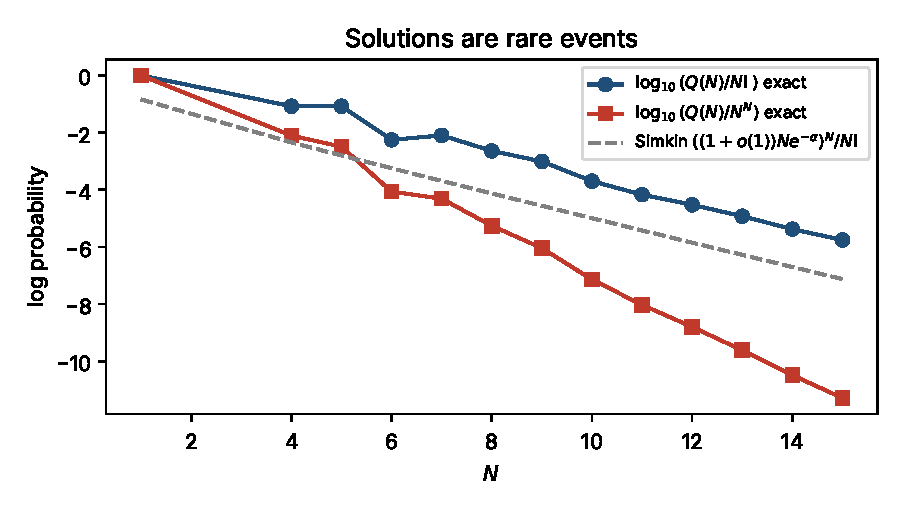
\includegraphics[width=0.95\textwidth]{fig_rarity.pdf}
\caption{The probability that a uniformly random permutation, or a uniformly random row placement, is a solution, on a logarithmic scale, for $N$ up to 15 (the values $N = 2, 3$, where there are no solutions, are omitted), together with Simkin's asymptotic (dashed, without the $o(1)$ correction).}
\label{fig:rarity}
\end{figure}

\section{Why the queens}

Several other problems could have served as our laboratory: the permanent of a zero one matrix, the number of perfect matchings in a graph, the number of satisfying assignments of a Boolean formula, the volume of a convex body. We chose the queens for three reasons.

The first is that it is a permutation problem with a natural energy. If $S(x)$ counts the number of attacking pairs in a placement, then $S$ takes integer values between zero and $\binom{N}{2}$, solutions are exactly the states of zero energy, and the whole structure of the problem is captured by the density of states\index{density of states} $N(s) = \#\{x : S(x) = s\}$. This makes the queens a Boltzmann system of exactly the kind studied in statistical physics, and we shall borrow freely from that field.

The second is that the problem is hard in every formal sense. The completion problem, in which some queens are already placed and one asks whether the placement extends to a solution, was shown by Gent, Jefferson and Nightingale \cite{GJN} in 2017 to be NP complete, and the corresponding counting problem to be $\sharpP$ complete. So a polynomial time algorithm for counting completions would be a polynomial time algorithm for everything in $\sharpP$, and since $\PH \subseteq \Pc^{\sharpP}$ by Toda's theorem \cite{Toda}, the whole polynomial hierarchy would collapse to $\Pc$.

The third is that the problem is concrete enough to compute with. For $N \le 9$ we can enumerate every permutation and tabulate the density of states exactly; for larger $N$ we have Simkin's asymptotics and decades of numerical experience. A theory of Monte Carlo counting that cannot be tested on the queens is not worth much.

\chapter{Counting as a Rare Event}
\label{ch:rare}

\section{The reformulation}

Let $\cX$ be a finite set of configurations and let $p$ be the uniform distribution on $\cX$. Let $S: \cX \to \{0, 1, 2, \dots\}$ be an energy, with the solutions being the states of zero energy. Then the number of solutions is
\[
Q = \#\{x : S(x) = 0\} = |\cX| \cdot \PP_p\big( S(x) = 0 \big) = |\cX| \cdot \EE_p\big[ \Ind_{\{S(x) = 0\}} \big] .
\]
Since $|\cX|$ is known analytically, counting is equivalent to computing a probability. For the queens with $\cX$ the set of row placements, $|\cX| = N^N$ and
\[
\rho_N = \PP_p\big( S(x) = 0 \big) = \frac{Q(N)}{N^N} ,
\]
so that for $N = 8$, $\rho_8 = 92 / 16\,777\,216 \approx 5.48 \times 10^{-6}$, while on the smaller space of permutations $\rho_8 = 92 / 40\,320 \approx 2.28 \times 10^{-3}$. This is the first key insight, used in this form by Diaconis\index{Diaconis and Holmes} and Holmes \cite{DiaconisHolmes} and to Rubinstein \cite{Rubinstein2006}: replace a counting problem with a rare event probability.

\section{Why naive Monte Carlo fails}

The obvious estimator draws $x^{(1)}, \dots, x^{(M)}$ independently from $p$ and sets
\[
\hat\rho = \frac{1}{M} \sum_{i=1}^{M} \Ind_{\{S(x^{(i)}) = 0\}} .
\]
It is unbiased with relative variance
\[
\frac{\Var(\hat\rho)}{\rho^2} = \frac{1 - \rho}{M \rho} ,
\]
so to achieve relative error $\epsilon$ one needs $M \approx 1/(\epsilon^2 \rho)$ samples. Since $\rho_N \approx e^{-1.942 N}$ this is exponential in $N$. Naive Monte Carlo is a correct algorithm with an exponential running time. The art of rare event simulation is the art of replacing this by something polynomial.

\section{The embedding principle}

One immediate improvement is to shrink the ambient space. Every solution is a permutation, so we may take $\cX$ to be the symmetric group $S_N$ with $|\cX| = N!$ and gain a factor of $N^N / N! \approx e^N$ in the rare event probability. This is the embedding principle: when the counting problem can be embedded in a smaller problem whose count is known, embed it. Rubinstein and Kroese \cite{RubinsteinKroese} embed the queens in the rooks problem, where any permutation is a solution, and ask for the fraction of rook solutions that are also queen solutions. The gain is exponential but the problem remains exponential, since $\rho_N \approx e^{-0.942 N}$ on permutations.

\section{The density of states}

The energy $S(x)$ for a permutation $x$ counts the attacking pairs,
\[
S(x) = \#\{ (i, j) : i < j, \; |x_i - x_j| = j - i \} .
\]
Table~\ref{tab:dos} records the density of states $N(s)$ for $N = 4$ to $9$, obtained by exhaustive enumeration. Several features will matter. The number of distinct energy levels is small, at most $1 + \binom{N}{2}$ and in practice much smaller. The distribution of energy has its mode near $N/2$ and a long, irregular right tail; the maximum energy $\binom{N}{2}$, in which every pair attacks, is attained only by the two main diagonals, and the levels just below it are empty. And the zero energy level, which is the one we want, sits at the far left of the distribution with an exponentially small share of the mass.

\begin{table}[t]
\centering
\small
\caption{Density of states $N(s)$, the number of permutations of $\{1,\dots,N\}$ with exactly $s$ attacking pairs, for $N = 4$ to $9$. Empty levels omitted.}
\label{tab:dos}
\begin{tabular}{rl}
\toprule
$N$ & $(s : N(s))$ \\
\midrule
4 & $0{:}2, \; 1{:}8, \; 2{:}6, \; 4{:}6, \; 6{:}2$ \\
5 & $0{:}10, \; 2{:}56, \; 4{:}42, \; 6{:}10, \; 10{:}2$ \\
6 & $0{:}4, \; 1{:}60, \; 2{:}160, \; 3{:}128, \; 4{:}188, \; 5{:}96, \; 6{:}24, \; 7{:}26, \; 8{:}8, \; 9{:}20, \; 11{:}4, \; 15{:}2$ \\
7 & $0{:}40, \; 1{:}152, \; 2{:}680, \; 3{:}1116, \; 4{:}960, \; 5{:}1000, \; 6{:}296, \; 7{:}498, \; 8{:}72,$ \\
  & $9{:}132, \; 11{:}66, \; 13{:}22, \; 15{:}4, \; 21{:}2$ \\
8 & $0{:}92, \; 1{:}888, \; 2{:}2864, \; 3{:}6872, \; 4{:}7892, \; 5{:}7552, \; 6{:}5658, \; 7{:}3448,$ \\
  & $8{:}2454, \; 9{:}968, \; 10{:}676, \; 11{:}496, \; 12{:}162, \; 13{:}72, \; 14{:}102, \; 15{:}16,$ \\
  & $16{:}62, \; 17{:}8, \; 18{:}32, \; 22{:}4, \; 28{:}2$ \\
9 & $0{:}352, \; 1{:}3376, \; 2{:}16648, \; 3{:}41016, \; 4{:}61980, \; 5{:}68728, \; 6{:}58864,$ \\
  & $7{:}41528, \; 8{:}30222, \; 9{:}15464, \; 10{:}11704, \; 11{:}4384, \; 12{:}4424, \; 13{:}968,$ \\
  & $14{:}1860, \; 15{:}144, \; 16{:}694, \; 17{:}104, \; 18{:}280, \; 20{:}22, \; 22{:}76, \; 24{:}36,$ \\
  & $28{:}4, \; 36{:}2$ \\
\bottomrule
\end{tabular}
\end{table}

\begin{figure}[t]
\centering
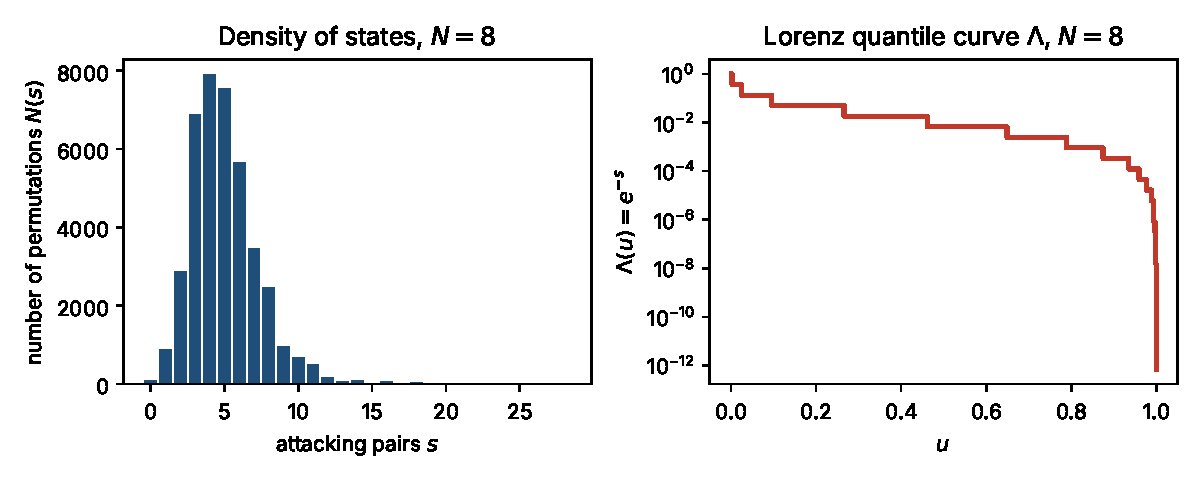
\includegraphics[width=\textwidth]{fig_dos8.pdf}
\caption{Left: the density of states for $N = 8$. Right: the quantile function $\Lambda(s)$ of the Boltzmann likelihood $L(x) = e^{-S(x)}$ under the uniform distribution on permutations. The solutions occupy the interval $[0, 92/40320)$ at the extreme left.}
\label{fig:dos8}
\end{figure}

\section{The Boltzmann view}

Attach to each permutation the Boltzmann weight $e^{-S(x)/\gamma}$ at temperature $\gamma$ and define the partition function
\[
Z(\gamma) = \sum_{x \in \cX} e^{-S(x)/\gamma} = \sum_{s \ge 0} N(s) e^{-s/\gamma} .
\]
As $\gamma \to 0$ the Boltzmann distribution $\pi_\gamma(x) = e^{-S(x)/\gamma} / Z(\gamma)$ concentrates on the ground states, which are the solutions, and $Z(\gamma) \to Q$. Counting is therefore computing a zero temperature limit of a partition function, and any method that computes partition functions, from simulated annealing\index{simulated annealing} to Wang and Landau, is a method for counting queens. The physicist's phrase for $\log N(s)$ is the microcanonical entropy; the complexity theorist's phrase for computing $N(0)$ is $\sharpP$. They are the same object seen from two sides, and the central claim of this book is that the quantile function of Monte Carlo is the bridge between them.

\chapter{Simkin's Theorem and the Queenon}
\label{ch:simkin}

Chapter~\ref{ch:gauss} stated Simkin\index{Simkin's theorem}'s theorem that $Q(N) = ((1 \pm o(1)) N e^{-\alpha})^N$ with $\alpha \approx 1.942$. This chapter describes how the theorem is proved and what the constant means, because the structure of the proof is itself a vertical argument: a lower bound from a sequential construction that is a ladder, and an upper bound from an entropy count that is a width.

\section{The upper bound: entropy}

Let $X$ be a uniformly random solution of the $N$ queens problem, encoded as the permutation $(x_1, \dots, x_N)$. Its entropy is $H(X) = \log Q(N)$, and the chain rule gives
\[
\log Q(N) = \sum_{i=1}^{N} H(x_i \mid x_1, \dots, x_{i-1}) .
\]
Each conditional entropy is at most the logarithm of the number of columns available to the queen in row $i$ given the earlier rows, and a column is available only if it is not already used and not attacked diagonally by any earlier queen. The trivial count, at most $N - (i-1)$ unused columns in row $i$, gives only $Q(N) \le N!$, that is $Q(N) \le (N e^{-1})^N$ up to a polynomial factor. This already gives the right form $(cN)^N$ but not the constant, since the truth is $c = e^{-\alpha}$ with $\alpha \approx 1.942$ rather than $1$. The diagonal constraints cannot be handled by subtracting attacked columns row by row, because the attacked columns overlap in a way that depends on the earlier placements.

Simkin's upper bound refines the count by conditioning on the empirical distribution of the solution on a coarse grid. Divide the board into $k \times k$ blocks and let $\nu$ be the matrix of block occupation numbers, which sums to $N$ and has row and column sums $N/k$. Given $\nu$, the entropy of $X$ is at most the entropy of a uniformly random placement with those block counts that respects the diagonal constraints within and between blocks, and this can be bounded by a sum over blocks of a local entropy term plus a correction for the diagonals. Letting $k \to \infty$ slowly with $N$, the bound becomes a functional of the limiting density $f(x, y)$ of queens on the unit square, and the best upper bound is the supremum of that functional over admissible $f$. The admissible limits are the queenon\index{queenon}s: permutons (probability measures on $[0,1]^2$ with uniform marginals in each coordinate, not necessarily with densities) that in addition satisfy the diagonal constraint that the mass on every diagonal and antidiagonal strip is at most the width of the strip, measured in the coordinate $x + y$ or $x - y$. For a queenon with density $f$ the functional is schematically
\[
\Psi(f) = -\int_{[0,1]^2} f \log f + \text{(diagonal terms)} ,
\]
where the first term is the entropy and the diagonal terms account for the requirement that each diagonal carry at most one queen. The best upper bound is the supremum of this functional over queenons, and the constant $\alpha$ is determined by that supremum. We do not reproduce Simkin's exact formula here (see \cite{Simkin}), and his numerical optimisation gives $\alpha = 1.942 \pm 0.003$.

\section{The lower bound: the random greedy ladder}

The matching lower bound is constructive. Place the queens one at a time in a random order of rows, choosing at each step a uniformly random column among those not attacked by the queens already placed, and analyse the number of available columns as the process runs. This is a random greedy algorithm, and Simkin shows that with the right choice of the queenon as a target distribution for the placements, and a careful analysis of the differential equations that govern the expected number of available positions, the algorithm succeeds in placing all but a vanishing fraction of the queens with probability bounded below, and the number of distinct outcomes is at least $((1 - o(1)) N e^{-\alpha})^N$. The argument uses the differential equations method of Wormald and an absorption step to complete the last few queens.

In our terms the random greedy algorithm is a ladder. Each row is a rung, the available columns at row $i$ are the level set $\{ x_i : S(x_1, \dots, x_i) = 0 \}$ given the earlier placements, and the number of outcomes is the product over rungs of the number of available choices. The lower bound is the product of the widths along the ladder, and the queenon is the choice of weight that makes the product as large as possible. This is the self reducibility route of Jerrum, Valiant\index{Valiant, Leslie} and Vazirani\index{Jerrum, Valiant and Vazirani}, row by row, and the differential equations are a deterministic approximation to the vertical walk in the limit $N \to \infty$. Simkin's proof is a derandomized vertical walk for the limiting problem.

\section{The queenon}

The optimising density $f^*$ is not uniform. Our own enumeration of the solutions for $N = 13$ (\texttt{code/queenon\_output.txt}, density normalised so that the uniform value is $1$) shows the density largest near the midpoints of the edges (about $1.42$) and below uniform both at the centre of the board (about $0.79$) and in the corners (about $0.49$). We do not offer an explanation of this pattern. A uniform solution is, in the limit, a sample from $f^*$ in the sense that its empirical distribution on any coarse grid converges to the block integrals of $f^*$.

This is a large deviations statement. The uniform distribution on permutations has, by Sanov's theorem and its permutation analogue, a limiting empirical density that is uniform on the square; conditioning on the rare event $S = 0$ tilts the limit to $f^*$. The tilt accounts for only part of the rate $\alpha - 1$: the remainder is the diagonal (no collision) term, which is paid even at the uniform density, as the independence estimate below suggests. The queenon is to the queens what the Wigner semicircle is to random matrices or the Vershik Kerov shape is to random Young diagrams: the limit shape under a hard constraint.

The queenon is not the optimal importance density for the vertical walk, which is the conditional law $p(\cdot \mid S = 0)$ of Chapter~\ref{ch:rareevent}; its one point marginals are only precursors of the queenon. A sampler that could draw permutations whose empirical density approximates $f^*$ would remove the part of the cost that is due to the tilt, but not the diagonal part, so the ground step would still have exponentially small probability. The cross entropy\index{cross entropy method} method of Chapter~\ref{ch:rareevent} with a product proposal having these marginals reduces the relative second moment of crude Monte Carlo by a factor of at most $e^{d}$, at most about $2$ for $7 \le N \le 12$ ($e^{0.68}$ at $N = 8$, while $N = 6$ gives $e^{2.43}$) (Chapter~\ref{ch:ce}), and queenon tilted swaps do not speed up the bottom rung chain (Chapter~\ref{ch:open}).

\section{The constant}

What is $\alpha$? It is defined by a variational problem and computed numerically to three decimals. No closed form is known and none is expected; the variational problem is infinite dimensional and its optimiser is not expressible in elementary terms. Simkin's bounds are $1.939 \le \alpha \le 1.945$. For comparison, if the pairs were independent with the mean of Chapter~\ref{ch:phase} the constant would be $1 + 2/3 = 1.667$; the gap of $0.275$ is the correlation correction.

For the walk the constant sets the length of the ladder: $\log(1/\rho_N) = (\alpha - 1) N + o(N) \approx 0.942 N$ on permutations, so with ratio $\tfrac12$ per rung one needs $1.36 N$ rungs. The experiments of Chapter~\ref{ch:experiments} used between five and nine rungs for $8 \le N \le 16$. Since the ratios along a ladder multiply to $\rho_N$, this forces a small average ratio: for $N = 16$, $\log(16!/Q(16)) \approx 14.2$ over nine rungs is an average ratio of about $0.21$, made up of ratios of $0.3$ to $0.6$ at the upper rungs and much smaller ones at the bottom (the final ratio is about $0.01$ at $N = 16$).

\section{Finite size corrections}

The $o(1)$ in Simkin's theorem is not small for the $N$ at which one can compute. From Table~\ref{tab:counts}, $\log_{10}(Q(N)/N!)$ decreases by $0.41$ per unit of $N$ above $N = 15$, matching $(\alpha - 1)/\ln 10 = 0.409$, but the intercept is off: the exact values are larger than $e^{-0.942 N}$ by a nearly constant factor, about $2.4$ for $15 \le N \le 27$. A natural guess is that $Q(N) / N! \sim C N^{\beta} e^{-(\alpha - 1) N}$ for constants $C$ and $\beta$, by analogy with the asymptotics of Latin squares and other constrained permutation counts, and the data up to $N = 27$ are consistent with $\beta = 0$ (Chapter~\ref{ch:open}). Establishing the polynomial correction would require a second order large deviations analysis around the queenon, which has not been done, and we record it among the open problems.


\chapter{Entropy, Types and the Rate Function of the Queens}
\label{ch:entropy}

The density of states\index{density of states} $N(s)$ is $e^{H(s)}$ for an entropy $H$, Simkin\index{Simkin's theorem}'s constant is an entropy, and the ladder length of the vertical walk is an entropy difference. This chapter gives the information theoretic view of the counting problem: the method of types, Sanov's theorem, the entropy chain rule as a counting tool, and the rate function for the number of attacking pairs in a random permutation, which we compute numerically from the exact density of states and conjecture as a variational problem over queenons.

\section{The method of types}

For a sequence of $n$ symbols from a finite alphabet, the type is the empirical distribution of symbols. There are at most $(n+1)^{|\mathcal{A}|}$ types, polynomially many, and the number of sequences of a given type $\nu$ is $\binom{n}{n \nu}$, which by Stirling is $e^{n H(\nu) + O(\log n)}$ where $H$ is the Shannon\index{Shannon, Claude} entropy. The probability of a type under an i.i.d. source $\mu$ is therefore $e^{-n D(\nu \| \mu) + O(\log n)}$, and Sanov's theorem states that the probability that the empirical distribution lies in a set $A$ is $e^{-n \inf_{\nu \in A} D(\nu \| \mu) + o(n)}$. Rare events are governed by the least improbable type that realises them, and the rate is a relative entropy.

Permutations are not i.i.d. sequences, but the method of types extends. A permutation of $[N]$ has a type in the sense of a block occupancy matrix on a $k \times k$ grid, normalised to sum to $1$, as in Simkin's proof, and the number of permutations with a given occupancy matrix $\nu$ is, by the asymptotics of the permanent\index{permanent} or by Stirling applied to the multinomial coefficients, $N! \, e^{-N D(\nu \| u_k) + o(N)}$ where $D(\nu \| u_k) = \sum_{ab} \nu_{ab} \log(k^2 \nu_{ab})$ is the relative entropy of $\nu$ from the uniform matrix $u_k$. The limiting objects as $k \to \infty$ are the doubly stochastic densities on the square, the permutons, and the queenon is a permuton.

\section{The entropy chain rule as a counting tool}

For a uniformly random solution $X = (x_1, \dots, x_N)$ the chain rule gives
\[
\log Q(N) = \sum_{i=1}^{N} H(x_i \mid x_1, \dots, x_{i-1}) ,
\]
and each term is at most the logarithm of the number of columns available to row $i$ given the earlier rows. This gives an upper bound on $Q(N)$ from any upper bound on the expected number of available columns, and it is the skeleton of Simkin's upper bound. In reverse, the vertical walk estimates each conditional entropy: the ratio $Z_{m_{t-1}} / Z_{m_t}$ is $e^{-\Delta H}$ for the entropy difference between consecutive level sets, and $\log \rho = \sum_t \log \theta_t$ is the total entropy drop from the uniform distribution on permutations to the uniform distribution on solutions. The ladder is a decomposition of an entropy into a sum of conditional entropies, each estimated by sampling, and the product estimator\index{product estimator}'s variance bound is a bound on how well a sum of $T$ conditional entropies can be estimated from $M$ samples each.

Shannon's source coding theorem gives this a concrete meaning. A uniformly random solution can be compressed to $\log_2 Q(N)$ bits and no fewer; a uniformly random permutation to $\log_2 N!$ bits; and the difference, $\log_2 (N! / Q(N))$, which is about $1.36 N$ bits by Simkin and the fit of Chapter~\ref{ch:open}, is the information that the constraint carries. The walk pays this many bits, in the form of rejected samples, to get from permutations to solutions, and $1.36 N$ bits at a ratio of one half per rung is $1.36 N$ rungs.

\section{The rate function of the attack count}

Let $S_N$ be the number of attacking pairs of a uniformly random permutation of $[N]$. Its mean is $2N/3 + O(1)$ by the calculation of Chapter~\ref{ch:phase}, and its distribution is concentrated: the variance is $O(N)$ by the pairwise structure, so the typical fluctuation is $O(\sqrt N)$. Large deviations ask for the probability that $S_N / N$ is near a value $e$ far from $2/3$, and the rate function is
\[
I(e) = -\lim_{N \to \infty} \frac{1}{N} \log \PP( S_N / N \approx e ) ,
\]
if the limit exists. Simkin's theorem gives $I(0) = \alpha - 1 = 0.942$. Nothing is proved about $I(e)$ for $e > 0$, and we offer a computation and a conjecture.

From the exact density of states for $N = 8$ to $11$, the function $-\log(N(s)/N!) / N$ against $s/N$ is plotted in Figure~\ref{fig:rate}. The curves for successive $N$ are close and converging to a convex curve with its minimum, zero, at $e \approx 0.65$ and value about $0.9$ at $e = 0$, with the finite size curves lying below the limit at $e = 0$ and rising towards it, as expected from the positive subexponential prefactor. The finite size minima sit at $e = 0.50$, $0.56$, $0.60$, $0.55$ for $N = 8$ to $11$, and the value $0.65$ is an extrapolation towards $2/3$. The curve rises steeply for $e$ above $1$, reflecting that configurations with many attacks are those near the main diagonals and are few.

\begin{figure}[t]
\centering
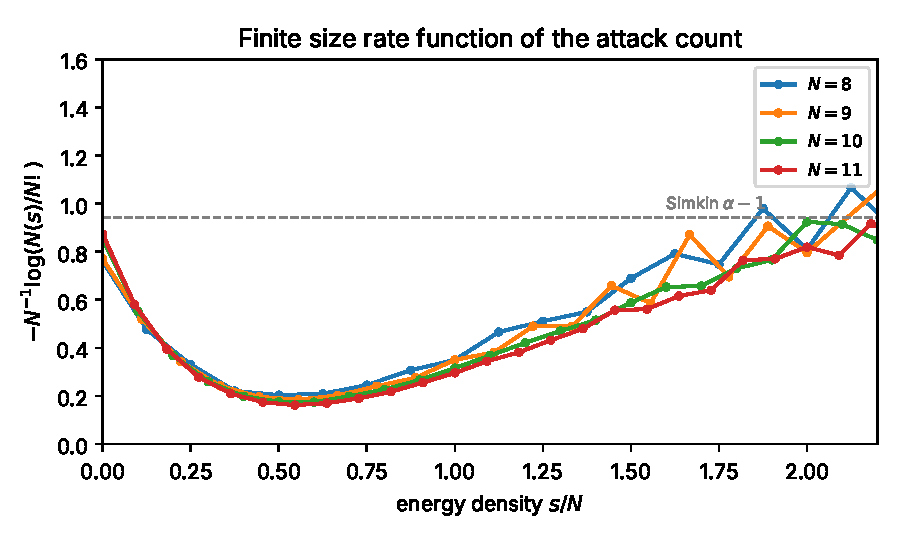
\includegraphics[width=0.85\textwidth]{fig_rate.pdf}
\caption{The finite size rate function $-N^{-1} \log(N(s)/N!)$ against the energy density $s/N$ for $N = 8$ to $11$, from the exact density of states. The curves converge to the large deviations rate function $I(e)$, with $I(0) = \alpha - 1 \approx 0.94$ by Simkin.}
\label{fig:rate}
\end{figure}

\begin{conjecture}
\label{conj:ratefn}
We conjecture that the rate function $I(e)$ exists, is convex on $[0, \infty)$ with $I(2/3) = 0$, and is given near $e = 0$ by a variational problem over queenon\index{queenon}like densities with prescribed attack density $e$ (queenons proper have $e = 0$): heuristically $I(e) = -\sup\{ \Psi(f) : f \text{ a queenon with attack density } e \}$ for the functional $\Psi$ of Simkin's upper bound (not the conductance of Chapter~\ref{ch:mixing}), suitably extended, so that $I(0) = \alpha - 1$. We do not prove this.
\end{conjecture}

The conjecture is the natural extension of Simkin's theorem from the ground state to every energy, and its proof would follow his method with the hard constraint of no attacks replaced by a soft constraint on the attack density. The payoff for the program is the staircase: the widths $N(s)/N!$ at energy $s = eN$ are $\exp(-N I(e) + o(N))$, and the vertical ladder's ratios are $\theta = \exp(-N (I(e - 1/N) - I(e))) \approx \exp(I'(e))$, so the ratio at each rung is the exponential of the slope of the rate function at that energy density, which is negative below the mode. At the bottom, $\theta_0 = \exp(I'(0))$, and the data of Chapter~\ref{ch:experiments} with $\theta_0 \approx 0.04$ to $0.01$ give $I'(0) \approx -3$ to $-4.6$, which is the sign and rough size of the slope the curve in Figure~\ref{fig:rate} shows at the origin. The caveat is that $\theta_0$ keeps falling with $N$ (exactly $0.094$, $0.094$, $0.048$, $0.038$ for $N = 8$ to $11$, and $0.01$ at $N = 16$), so these data give no evidence that $-\log \theta_0$ converges to a finite $-I'(0)$. To the extent that the conjecture holds, the rate function governs the ladder; we have not shown that it does.

\section{Entropy and mixing}

There is a further connection, between entropy and mixing, that is at the frontier of the subject. The modified log Sobolev inequality for a Markov chain bounds the rate at which the relative entropy of the chain's distribution from stationarity decreases, and gives mixing time bounds that are often sharper than those from conductance\index{conductance}. For chains on the symmetric group under transpositions, the log Sobolev constant is known by the work of Diaconis\index{Diaconis and Saloff Coste} and Saloff Coste, and the random transposition walk mixes in $\tfrac12 N \log N$ steps with a cutoff. The swap chain on a level set is the random transposition walk restricted to a subset, and if the subset has good isoperimetry the restriction inherits a log Sobolev constant and mixes in $O(N \log N)$ times a factor depending on the restriction. The measured $N^{1.8}$ of Chapter~\ref{ch:experiments2} is consistent with $N \log N$ times a slowly growing factor, or with a genuine power. Distinguishing these would need data to larger $N$, and a proof would need the isoperimetry of the giant component.

\section{What entropy tells the program}

Entropy gives the program its accounting. The walk must pay $\log N! - \log Q(N)$ nats, about $0.94 N$, to reach the solutions, the ratio at each rung is the local slope of the rate function, the number of rungs is the total drop divided by the mean slope, and the cost per rung is the mixing time at that energy. The first three are properties of the staircase and are polynomial provided a ladder with every ratio bounded below exists, which we have not shown. The fourth is a property of the chain, and the entropy method says what it would take to bound it: a log Sobolev or isoperimetric inequality on the level set. For the unconditioned queens we have the giant component\index{giant component} and the measured exponent; for the conditioned queens we have neither, and the entropy accounting says only that the bill, if the level set shatters, is exponential.


\chapter{Latin Squares and Other Permutation Counts}
\label{ch:latin}

The queens are one of a family of counting problems on permutations in which an explicit constraint cuts an exponentially small fraction out of $N!$, and the family has a shared asymptotic theory, a shared set of methods, and a shared open question about constants. This chapter surveys the family: derangements, where everything is exact; Latin squares, where the leading constant is known and the lower order terms are open; the toroidal queens, where the count is a number theoretic function; and the general permanent of a zero one matrix, where the van der Waerden and Br\`egman bounds frame everything.

\section{Derangements and the rook polynomial}

A derangement is a permutation with no fixed point, and the number $D(N)$ of derangements is $N!$ times $\sum_{k=0}^{N} (-1)^k / k!$, which is $N!/e$ rounded to the nearest integer. The count is exact by inclusion exclusion, and the ratio $D(N)/N! \to 1/e$ is the simplest instance of a rare event in permutations that is not rare: a constant fraction. More generally, for a board $B$ of forbidden squares, the number of permutations avoiding $B$ is $\sum_k (-1)^k r_k(B) (N - k)!$ where $r_k$ is the number of ways to place $k$ non attacking rooks on $B$, the rook polynomial of Kaplansky and Riordan. For the queens the forbidden structure is not a fixed set of squares but a set of pairs, which is why inclusion exclusion does not close and the problem is $\sharpP$ hard.

\section{Latin squares}

A Latin square of order $n$ is an $n \times n$ array over $n$ symbols with each symbol once in each row and column; equivalently it is a sequence of $n$ permutations that are pairwise disjoint as sets of positions. The number $L(n)$ is known exactly only to $n = 11$, where it is about $7.8 \times 10^{47}$, and the leading asymptotics follow from the van der Waerden and Br\`egman inequalities on permanents, as presented by van Lint and Wilson, which give
\[
L(n)^{1/n^2} \sim \frac{n}{e^2} ,
\]
so that $\log L(n) = n^2 \log n - 2 n^2 + o(n^2)$. The constant $e^{-2}$, the analogue of Simkin's constant for the queens, is known; the lower order terms are not: van der Waerden's inequality and Br\`egman's inequality, applied row by row, pin $\log L(n)$ to $n^2 \log n - 2n^2 + o(n^2)$ and leave the terms of order $n \log n$ and $n$ open. Keevash's existence and counting theorems for designs, and the refinements of Kwan, Sah, Sawhney and Simkin on substructures in Latin squares, sharpen the error term and count Latin squares with prescribed structure, but the constant in the next order remains unidentified.

The method of the Latin square counts is the method of the queens: entropy upper bounds via the chain rule, applied row by row, and random greedy or absorption lower bounds. Simkin's queens paper is explicitly in this tradition and borrows the technology of the Latin square and design counts. The queens differ in that the constraint is between every pair of rows at once rather than between a row and the set of previous rows, which is what makes the queens a model with a nontrivial limit object, the queenon, where the Latin square limit is trivial.

\section{Toroidal queens}

Place the queens on a torus, so that the diagonals wrap around. The number of toroidal solutions $T(N)$ is zero unless $\gcd(N, 6) = 1$, by a theorem of P\'olya from 1918, and for such $N$ the linear permutations $x_i = a i + b \bmod N$ with $a$, $a - 1$ and $a + 1$ all coprime to $N$ are solutions, which already gives a count growing nearly quadratically in $N$; the exact values are known for small $N$ and grow as $((1 + o(1)) N e^{-\alpha_T})^N$ for a toroidal constant $\alpha_T \ge \alpha$, since every toroidal solution is a planar solution. The torus is strictly rarer, and its constant is known: Luria~\cite{Luria2017} proved the upper bound $T(N) \le ((1 + o(1)) N e^{-3})^N$, and Bowtell and Keevash~\cite{BowtellKeevash} proved the matching lower bound for $\gcd(N, 6) = 1$, so that $\alpha_T = 3 > \alpha \approx 1.942$. This is what the translation invariant variational problem on the torus suggests, with the uniform density as optimiser, and it is one of the few exact constants in the family.

The toroidal problem also has a level set structure that is more symmetric than the planar one, since the dihedral symmetry of the square is replaced by the affine group of the torus, and the swap chain on toroidal level sets should mix at least as well. We have not run it.

\section{The permanent and its bounds}

The permanent of a zero one $N \times N$ matrix $A$ counts the permutations supported on the ones of $A$, and derangements and permutations avoiding a board are permanents. The two classical inequalities are van der Waerden's, proved by Egorychev and Falikman in 1981, that a doubly stochastic matrix has permanent at least $N! / N^N$, and Br\`egman's of 1973, that a zero one matrix with row sums $r_i$ has permanent at most $\prod_i (r_i!)^{1/r_i}$. Together they bracket the number of permutations avoiding a given forbidden board to within a factor exponential in $N$, which is the precision of the leading order asymptotics for Latin squares and for every other problem of the family. The queens are not a single permanent, because the constraint is on pairs of positions rather than on a fixed board, and the standard expansion is an inclusion exclusion over sets of attacking pairs, which has no permanent structure.

Jerrum, Sinclair and Vigoda's FPRAS for the permanent, discussed in Chapter~\ref{ch:labs}, applies to every single permanent in the family and so gives a polynomial time approximation for derangements, for permutations avoiding any fixed board, and for the number of ways to extend a Latin rectangle by one row. It does not apply to the queens, whose inclusion exclusion over attacking pairs has exponentially many terms with alternating signs, and the alternation is what defeats the method: the FPRAS for a sum with cancellation is not a sum of FPRAS for the terms. This is, from the permanent side, the reason the queens are harder than derangements and the other single permanents of the family.

\section{The constants}

Every problem in the family has an asymptotic of the form $( (1 + o(1)) N c )^N$ or $( (1 + o(1)) n c )^{n^2}$ with an explicit $c$: $1/e$ for derangements, $1/e^2$ for Latin squares, $e^{-\alpha}$ for the queens. The first is exact by inclusion exclusion. The second is exact by van der Waerden and Br\`egman. The third is a variational constant computed numerically and not known in closed form, and the difference is that the queens have a nontrivial limit object. The family suggests that the right question about $\alpha$ is not its decimal expansion but whether it is the value of a recognisable functional at a recognisable density, in the way that $1/e^2$ is the value of the Br\`egman bound at the uniform doubly stochastic matrix. Simkin's queenon is the density; the functional is his; and the question whether $\alpha$ can be identified is the question whether the queenon can be. We record it among the open problems of Chapter~\ref{ch:open} under the finite size and rate function headings.


\part{Monte Carlo Counting}

\chapter{Product Estimators and Annealing}
\label{ch:product}

\section{Splitting a rare event}

If a rare event cannot be hit directly, approach it in stages. Let $S$ be the energy and define, for each level $m$,
\[
Z_m = \PP_p\big( S(x) \le m \big) , \qquad Z_\infty = 1, \quad Z_0 = \rho .
\]
Choose a ladder of levels $m_0 = 0 < m_1 < \dots < m_T = \infty$ and write the telescoping product
\[
\rho = Z_0 = \prod_{t=1}^{T} \frac{Z_{m_{t-1}}}{Z_{m_t}} .
\]
Each ratio $Z_{m_{t-1}} / Z_{m_t} = \PP_p(S \le m_{t-1} \mid S \le m_t)$ is a conditional probability which, if the levels are well spaced, is not small, and so can be estimated by ordinary Monte Carlo from samples of $p$ conditioned on $\{S \le m_t\}$. This is the product estimator of Jerrum, Valiant and Vazirani\index{Jerrum, Valiant and Vazirani} in the counting literature and the splitting method of Kahn and Harris in rare event simulation; Diaconis and Holmes give a clear account of it with the queens in mind.

For the queens with $N = 8$ the exact values $Z_m$ on permutations, from Table~\ref{tab:dos}, run
\[
\begin{gathered}
Z_0 = 0.00228, \; Z_1 = 0.0243, \; Z_2 = 0.0953, \; Z_3 = 0.266, \\ Z_4 = 0.462, \; Z_5 = 0.649, \; Z_6 = 0.789, \dots
\end{gathered}
\]
so that with every integer level used, the first ratio $Z_0 / Z_1 = 0.094$ is the smallest and the rest are between $0.25$ and $1$. Nothing is rare any more; the difficulty has moved into producing samples from the conditioned distributions.

\section{Variance of the product}

Suppose each ratio $\theta_t = Z_{m_{t-1}} / Z_{m_t}$ is estimated by an independent $\hat\theta_t$ with mean $\theta_t$ and relative variance $c_t^2 = \Var(\hat\theta_t) / \theta_t^2$. Then $\hat\rho = \prod_t \hat\theta_t$ is unbiased and
\[
\frac{\Var(\hat\rho)}{\rho^2} = \prod_{t=1}^{T} (1 + c_t^2) - 1 .
\]
If each ratio is estimated by $M_t$ Bernoulli samples then $c_t^2 = (1 - \theta_t) / (M_t \theta_t)$, and if all $\theta_t$ are bounded below by a constant and $M_t = M$ then the relative variance is at most $e^{T C / M} - 1$, which is $O(\epsilon^2)$ when $M$ is of order $T / \epsilon^2$. The total sample size is $O(T^2 / \epsilon^2)$.

The length $T$ of the ladder is therefore the governing quantity. Since each ratio is at most one and the product is $\rho$, a ladder with all ratios at least $\tfrac12$ has length at least $\log_2(1/\rho)$, and the analysis above needs a ladder of length $O(\log(1/\rho))$ with every ratio bounded below by a constant. For the queens $\log(1/\rho_N) \approx 0.942 N$ on permutations, so a ladder with ratios at least $\tfrac12$ has at least $1.36 N$ rungs, and if one of length $T = O(N)$ exists the total sample complexity is $O(N^2 / \epsilon^2)$ times the cost of producing one conditioned sample. We have not shown that such a ladder exists. For the integer ladder the bottom ratio is not bounded below: the exact values of $Z_0 / Z_1$ are $0.094$, $0.094$, $0.048$, $0.038$ for $N = 8, \dots, 11$, and about $0.01$ at $N = 16$. Keeping every ratio bounded below would require splitting the bottom rung by non integer or tempered levels, at a cost we do not analyse. Granting such a ladder, and a polynomial cost for producing one conditioned sample, the scheme is polynomial.

\section{Well balanced schedules}

The classical analysis, with Chebyshev's inequality in place of exact variances, gives a sample complexity of $O\big( (\ln(1/\rho))^2 \epsilon^{-2} \big)$ for a ladder in which every ratio is bounded away from zero and one, the well balanced schedule of Dyer and Frieze. \v{S}tefankovi\v{c}, Vempala and Vigoda showed in 2009 that an adaptive schedule can do better: for the partition function $Z(\beta) = \sum_s N(s) e^{-\beta s}$ a cooling schedule of length $O^*\big( \sqrt{\ln Z(0)} \big)$ suffices, where $O^*$ hides logarithmic factors, and Huber \cite{Huber} later reduced the logarithmic overhead in the total number of samples to a $\ln \ln$ factor with a paired product estimator\index{product estimator}. The improvement of \v{S}tefankovi\v{c}, Vempala and Vigoda does not come from ratios close to one (with a schedule that short the typical ratio is far from one); it comes from bounding the relative variance of the estimator of each step even when the mean ratio is small.

The point to retain is that the ladder length is governed by the logarithm of the rare event probability, which is linear in $N$ for the queens, and is not the obstruction once a ladder with every ratio bounded below is granted. What may be the obstruction, and in general is, is the cost of each conditioned sample.

\section{Simulated annealing and the Boltzmann ladder}

Instead of conditioning on hard level sets one may soften them. The Boltzmann distribution $\pi_\gamma(x) \propto e^{-S(x)/\gamma}$ interpolates between the uniform distribution at $\gamma = \infty$ and the uniform distribution on solutions at $\gamma = 0$, and
\[
\frac{Q}{|\cX|} = \lim_{\gamma \to 0} \frac{Z(\gamma)}{Z(\infty)} = \lim_{\gamma \to 0} \prod_{k} \frac{Z(\gamma_k)}{Z(\gamma_{k-1})}
\]
along any sequence $\gamma_0 = \infty > \gamma_1 > \dots \to 0$. Each ratio is
\[
\frac{Z(\gamma_k)}{Z(\gamma_{k-1})} = \EE_{\pi_{\gamma_{k-1}}}\Big[ e^{-S(x)(1/\gamma_k - 1/\gamma_{k-1})} \Big] ,
\]
an expectation under the previous Boltzmann distribution that is estimated by sampling from it, typically by Metropolis\index{Metropolis algorithm} or Gibbs moves that swap two queens. This is simulated annealing in the sense of Kirkpatrick, Gelatt and Vecchi used for estimation rather than optimisation, and it is the route taken by Rubinstein and Kroese, who define $S$ as a threat count and run a Gibbs sampler to its minimum.

Annealing can meet a phase transition. As $\gamma$ decreases the Boltzmann distribution shifts from the bulk of the density of states, around $s \approx N/2$, towards the ground state, and at some temperature the number of low energy states that the chain can reach may change abruptly. Controlling the rate at which $\gamma$ decreases through this transition is exactly the problem of choosing the ladder, and is the problem that the vertical likelihood weight function $\Omega$ of Chapter~\ref{ch:vertical} is designed to solve.

\section{The cross entropy method}

Rubinstein's cross entropy\index{cross entropy method} method is an adaptive importance sampling scheme for the same problem. One seeks, within a parametric family $h_v$, the density closest in Kullback Leibler divergence to the optimal zero variance importance density
\[
g^*(x) = \frac{p(x) \, \Ind_{\{S(x) \le m\}}}{Z_m} .
\]
The divergence $D(g^* \| h_v) = \EE_{g^*} \log( g^* / h_v )$ is minimised over $v$, which for exponential families reduces to matching sufficient statistics on the elite samples, those with $S \le m$. The level $m$ and the parameter $v$ are then updated together, with $m$ lowered to a fixed quantile of the current sample at each stage. The method is elegant and effective in practice; its theoretical guarantees are weaker than those of the product estimator because the parametric family may not be rich enough to approximate $g^*$ as $m \to 0$.

\chapter{Markov Chains and Mixing Times}
\label{ch:mixing}

Every conditioned draw in the vertical walk is produced by a Markov chain. The number of steps the chain needs before its state is nearly uniform on the level set is the mixing time, and it is the quantity that decides whether the walk is polynomial. This chapter collects the theory of mixing that the rest of the book relies on: the spectral gap, conductance and Cheeger's inequality, canonical path\index{canonical paths}s, coupling, and the particular difficulties of chains on level sets.

\section{Chains, stationarity and reversibility}

Let $\cX$ be a finite state space and $P$ a transition matrix, $P(x, y) \ge 0$, $\sum_y P(x, y) = 1$. A distribution $\pi$ is stationary if $\pi P = \pi$. The chain is irreducible if every state is reachable from every other, aperiodic if the greatest common divisor of return times is one, and ergodic if both; an ergodic chain has a unique stationary distribution and $P^t(x, \cdot) \to \pi$ for every $x$. The chain is reversible with respect to $\pi$ if $\pi(x) P(x, y) = \pi(y) P(y, x)$ for all $x, y$, the detailed balance condition. Metropolis\index{Metropolis algorithm} chains and random scan Gibbs chains are reversible by construction.

The Metropolis chain for a target $\pi$ on permutations with symmetric proposal $q$ moves from $x$ to a proposed $y \sim q(x, \cdot)$ and accepts with probability $\min\{1, \pi(y) / \pi(x)\}$. For the uniform distribution on a level set $\{ S \le m \}$ the acceptance probability is one if $S(y) \le m$ and zero otherwise: the chain proposes a swap of two queens and makes it if the energy stays below the level. This is the chain used in the experiments of Chapter~\ref{ch:experiments}. It is reversible with respect to the uniform distribution on the level set, and it is irreducible if and only if the level set is connected under swaps.

\section{Total variation and mixing time}

The distance of the chain from stationarity after $t$ steps, started from $x$, is
\[
d_x(t) = \| P^t(x, \cdot) - \pi \|_{TV} = \tfrac12 \sum_y |P^t(x, y) - \pi(y)| ,
\]
which also equals $\max_{A \subseteq \cX} | P^t(x, A) - \pi(A) |$, and the mixing time\index{mixing time} is
\[
\tau(\epsilon) = \min\{ t : \max_x d_x(t) \le \epsilon \} .
\]
A standard submultiplicativity argument shows that $\tau(\epsilon)$ is at most $\tau(\tfrac14) \lceil \log_2(1/\epsilon) \rceil$, so the dependence on $\epsilon$ is logarithmic and one speaks of the mixing time $\tau = \tau(\tfrac14)$. A chain on an exponentially large state space mixes rapidly if $\tau$ is polynomial in the size of the problem description, here $N$.

The definition of a polynomial level set sampler\index{level set sampler} in Chapter~\ref{ch:prp} asks for a sample within total variation $\delta$ of uniform in time polynomial in $N$ and $\log(1/\delta)$. By the submultiplicativity bound this is achieved by a rapidly mixing chain on each level set, together with a polynomial time way to find a starting state in the level set. For the queens a starting state in $\{ S \le m \}$ is easy to find for $m$ in the bulk, by rejection, and for $m$ near zero on a partially filled board the starting state is itself an $\NP$ hard problem (on the empty board explicit solutions exist for every $N \ge 4$); the vertical walk attempts it by inheriting the starting state from the previous level, which is the whole point of the ladder.

\section{The spectral gap}

For a reversible chain the matrix $P$ is self adjoint on $L^2(\pi)$ with real eigenvalues $1 = \lambda_1 > \lambda_2 \ge \dots \ge \lambda_{|\cX|} \ge -1$. The spectral gap\index{spectral gap} is $\gamma = 1 - \lambda_2$ and the absolute spectral gap is $\gamma_* = 1 - \max\{\lambda_2, |\lambda_{|\cX|}|\}$; making the chain lazy, $P \to (I + P)/2$, forces all eigenvalues nonnegative and halves the gap. The relaxation time is $t_{rel} = 1/\gamma_*$, and the standard bounds are
\[
(t_{rel} - 1) \log \frac{1}{2\epsilon} \le \tau(\epsilon) \le t_{rel} \log \frac{1}{\epsilon \, \pi_{min}} ,
\]
where $\pi_{min} = \min_x \pi(x)$. For the uniform distribution on a level set of size $|\cX_m|$ the upper bound reads $\tau \le t_{rel} ( \log |\cX_m| + \log(1/\epsilon) )$, and $\log |\cX_m| \le \log N! = O(N \log N)$, so a polynomial relaxation time gives a polynomial mixing time.

\section{Conductance and Cheeger's inequality}

The spectral gap is hard to compute directly on an exponentially large space. Jerrum and Sinclair's method is to bound it by the conductance\index{conductance}, a geometric quantity. For $A \subseteq \cX$ with $\pi(A) \le \tfrac12$ let
\[
\Phi(A) = \frac{F(A, A^c)}{\pi(A)} , \qquad F(A, B) = \sum_{x \in A, y \in B} \pi(x) P(x, y) ,
\]
be the probability of leaving $A$ in one step from stationarity, conditional on being in $A$, and let $\Phi = \min_{\pi(A) \le 1/2} \Phi(A)$ be the conductance of the chain. Cheeger\index{Cheeger's inequality}'s inequality for Markov chains, due in this form to Jerrum and Sinclair and to Lawler and Sokal, states
\[
\frac{\Phi^2}{2} \le \gamma \le 2 \Phi .
\]
A chain mixes rapidly if and only if its conductance is at least inverse polynomial: there is no set of stationary mass at most a half from which the chain escapes with probability less than $1/\mathrm{poly}(N)$ per step. The failure of mixing is always a bottleneck, a set $A$ with small boundary relative to its mass, and the level sets of the queens energy are suspected to have exactly such bottlenecks at low energy, where, on partially filled boards, the components under swap moves are suspected to be isolated and scattered (on unconditioned boards the exact data show a giant component, below).

\section{Canonical paths}

Jerrum and Sinclair's technique for lower bounding the conductance is to route a flow between every pair of states along a canonical path and to bound the congestion of the routing. For each pair $(x, y)$ choose a path $\Gamma_{xy}$ in the transition graph, and define the congestion
\[
\kappa = \max_{(u, v) : P(u, v) > 0} \frac{1}{\pi(u) P(u, v)} \sum_{(x, y) : (u, v) \in \Gamma_{xy}} \pi(x) \pi(y) \, |\Gamma_{xy}| .
\]
Then $\gamma \ge 1 / \kappa$, and so, for a lazy chain, for which $\gamma_* = \gamma$, $t_{rel} \le \kappa$. The congestion is small if the paths are short and spread evenly over the edges, which in practice means exhibiting an injection from the set of pairs $(x, y)$ whose paths use a given edge into the state space, with a small loss. This is the technique that proved rapid mixing for the permanent\index{permanent} of dense matrices and for the ferromagnetic Ising model, and its refinement by Jerrum, Sinclair and Vigoda, with weights on the states to balance the congestion, proved rapid mixing for the permanent in general.

For the queens the canonical path method would require, for each pair of placements in a level set, a sequence of swaps staying within the level set, and a bound on how many pairs route through any one swap. For $m$ in the bulk this is plausible and we expect it can be carried out. For $m$ near zero on an unconditioned board the exact data of Chapter~\ref{ch:open} show that almost all solutions lie in one component of $\{ S \le 1 \}$ (all of them at $N = 8$, $10$, $11$; all but $4$ of $14200$ at $N = 12$), so the first requirement is plausible there, and the method is open rather than inapplicable. On partially filled boards, which is where the conjecture of Chapter~\ref{ch:prp} lives, the components are scattered and the method does not apply, which is evidence for that conjecture and no more.

\section{Coupling}

The coupling\index{coupling} method bounds mixing by constructing two copies of the chain, started from different states, run jointly so that each is marginally a copy of $P$ and so that once they meet they stay together. If $T$ is the meeting time then $d_x(t) \le \max_y \PP(T > t)$, where $y$ is the starting state of the second copy, and the mixing time is bounded by the tail of $T$. The path coupling theorem of Bubley and Dyer reduces the construction to adjacent pairs of states: if a metric on $\cX$ can be found such that for every pair at distance one there is a one step coupling that contracts the expected distance by a factor $1 - \beta$, then $\tau(\epsilon) \le \beta^{-1} \log( D / \epsilon )$ where $D$ is the diameter. Coupling proved rapid mixing for graph colourings with enough colours, for independent sets at low density, and for many spin systems above their critical temperature.

For a level set chain on permutations the natural metric is the number of transpositions separating two permutations, and the natural coupling makes the same swap proposal in both copies. The coupling contracts if, on average, a proposed swap is accepted in both copies or rejected in both; it fails to contract when one copy accepts and the other rejects, which happens when the swap crosses the level in one copy but not the other. At high levels this is rare and the coupling contracts; at low levels it is the norm.

\section{Slow mixing: torpidity}

A chain is torpid\index{torpid mixing}ly mixing if its mixing time is exponential. The standard proof is to exhibit a bottleneck: a set $A$ with $\pi(A) \le \tfrac12$ and $\Phi(A)$ exponentially small, from which Cheeger's inequality gives an exponentially small gap. Gore and Jerrum\index{Gore and Jerrum}'s proof that Swendsen\index{Swendsen Wang algorithm} Wang mixes torpidly on the complete graph at the Potts critical temperature exhibits the bottleneck between the ordered and disordered phases: the chain must pass through configurations of mixed magnetisation that have exponentially small weight. Borgs, Chayes and others showed the same for the Ising model on the torus below the critical temperature with single site dynamics. In every case the bottleneck is a phase coexistence, and the chain's inability to cross it is the dynamical manifestation of a first order transition.

For the queens we conjecture a bottleneck of a different kind, not between two phases but among exponentially many components of a low level set. There is no magnetisation to measure, and the components are not related by any symmetry; they are simply the connected pieces of $\{ S \le m \}$ under swaps, and on partially filled boards we believe that for $m = O(1)$ there are exponentially many of them, each of size polynomial in $N$. On unconditioned boards the exact data show the opposite, a giant component. A chain confined to swaps cannot leave its component. A chain with nonlocal moves, such as the cluster moves of Swendsen Wang on the row column bipartite graph, may leave it, and the question is whether it leaves it fast enough.

\section{Frieze, Kannan and Polson: log concave sampling}

One of the first results showing a Metropolis chain mixing in polynomial time on a continuous space of high dimension is due to Frieze, Kannan and Polson\index{Frieze, Kannan and Polson} in 1994, sharpening Applegate and Kannan (1991). Let $f$ be a log concave density on a convex body $K \subseteq \mathbb{R}^d$, and consider the random walk that from $x$ proposes a uniformly random point $y$ in the ball of radius $r$ about $x$, and accepts with probability $\min\{1, f(y) / f(x)\}$, rejecting proposals that leave $K$. Frieze, Kannan and Polson proved that, for $r$ of order $1/\sqrt d$ and a suitable warm start, the chain reaches total variation distance $\epsilon$ from $f$ in a number of steps polynomial in $d$, the diameter of $K$, and $\log(1/\epsilon)$. The proof establishes an isoperimetric inequality for log concave measures, that any partition of $K$ into two parts of substantial mass has a boundary of substantial measure, and converts it into a conductance bound for the ball walk by the Jerrum Sinclair argument; the localisation lemma of Lov\'asz\index{Lov\'asz, L\'aszl\'o} and Simonovits is the tool for the isoperimetry.

The result matters for this book in three ways. It is among the first mixing bounds for a Metropolis chain as statisticians use it, with a continuous target and an accept reject step, and it placed Bayesian posterior sampling for log concave posteriors in the class of problems with polynomial time randomized algorithms. It continues the Dyer Frieze Kannan volume algorithm, extended from indicators to densities by Applegate and Kannan and then sharpened, so that the vertical ladder for the evidence of a log concave model inherits a polynomial guarantee at every rung. And it is the template for what a mixing proof for the queens would look like: an isoperimetric inequality on the level set, showing that no subset of half the mass has a small boundary under swaps, converted to conductance. For convex bodies the isoperimetry comes from convexity. For the queens level sets there is no convexity, and the giant component\index{giant component} structure of Chapter~\ref{ch:open} is the closest available substitute: the solutions are bridged by near solutions, and an isoperimetric inequality for the bridged graph would give polynomial mixing on unconditioned boards.

\section{The Polson 1996 criterion}

One of us, in a 1996 discussion paper on the convergence of Markov chain Monte Carlo, gave conditions for geometric ergodicity of Gibbs and Metropolis chains in terms of drift conditions and small sets, and emphasised that the rate of convergence of a chain used for a Bayesian computation is governed by the same spectral quantities as a chain used for counting. The point of the paper was that the statistical and the complexity theoretic analyses of Markov chains were the same analysis, and that the rapid mixing bounds of Jerrum and Sinclair could be read as statements about the convergence of Bayesian posterior samplers. Thirty years later the point stands and has been sharpened by the vertical view: the chain that samples a level set for counting is the chain that samples a likelihood slice for posterior inference, and the ladder of levels in the counting problem is the ladder of likelihood thresholds in nested sampling\index{nested sampling}. Mixing time analysis is the common currency.

\section{What mixing means for the thesis}

The thesis of Chapter~\ref{ch:prp} places the whole hardness of counting in the widths of a staircase, and this chapter places the whole hardness of estimating a width in the mixing time of a chain on a level set. The two statements are the same statement. A width $N(s) / |\cX|$ is the stationary mass of the energy shell $\{ S = s \}$, and the mass of a level set $\{ S \le m \}$ is the sum of the widths below $m$; its estimate from conditioned samples is unbiased if the samples are stationary and biased by the total variation distance otherwise; the number of samples needed is polynomial provided the ratios between consecutive levels are bounded below, which we have not shown for the queens; the number of chain steps per sample is the mixing time. If the mixing time is polynomial for every level then the walk is an FPRAS\index{FPRAS} and, for the queens completion count, $\NP = \RP$. If it is exponential for some level then the walk is an exponential algorithm and the thesis says only where the exponential is hiding. We believe the latter. We would be delighted to be wrong.


\chapter{Convergence of MCMC and the Witch's Hat}
\label{ch:witchhat}

Every level set sampler in this book is a Markov chain Monte Carlo algorithm, and the question of its mixing is the question statisticians have asked about Gibbs and Metropolis samplers since the late 1980s. This chapter gives the statistical side of that story: the Gibbs sampler and the Metropolis Hastings algorithm as they are used in Bayesian inference, the Peskun ordering, the convergence theory of Tierney and of Meyn and Tweedie, the diagnostics of Gelman and Rubin and of Geyer, and the witch's hat example which showed that a chain can look converged while being exponentially far from it. The witch's hat is, in miniature, the problem of the bottom rung.

\section{Gibbs and Metropolis Hastings}

The Gibbs sampler, named by Geman and Geman in 1984 and brought into mainstream statistics by Gelfand and Smith in 1990, updates a vector $x = (x_1, \dots, x_d)$ one coordinate at a time, drawing $x_i$ from its conditional distribution given the rest. Each update leaves the target invariant, and the chain is reversible if the coordinates are updated in random order. The level set chain for the queens is a Metropolis chain on pairs of coordinates: a swap of rows $i$ and $j$ proposes the other order of $(x_i, x_j)$ and accepts if the energy stays below the threshold. The Gibbs sampler on the pair, which draws $(x_i, x_j)$ from its conditional given the other rows, uniform on the at most two admissible values, is the lazy version of this chain: it swaps with probability $1/2$ when both orders are admissible.

The Metropolis Hastings algorithm, from Metropolis and coauthors in 1953 and Hastings in 1970, proposes $y \sim q(x, \cdot)$ and accepts with probability
\[
\alpha(x, y) = \min\Big\{ 1, \, \frac{\pi(y) \, q(y, x)}{\pi(x) \, q(x, y)} \Big\} ,
\]
which makes the chain reversible with respect to $\pi$ for any proposal $q$. Gibbs is the special case in which the proposal is the conditional and the acceptance is always one. The block chain of Chapter~\ref{ch:swendsen} is Metropolis Hastings with a block proposal, and the generator proposes and chain corrects loop of Chapter~\ref{ch:gbc} is Metropolis Hastings with a learned proposal.

\section{Peskun's ordering}

Peskun showed in 1973 that among reversible chains with the same stationary distribution, one that moves more, in the sense that its off diagonal transition probabilities dominate those of another, has smaller asymptotic variance for every function. The Metropolis acceptance rule is optimal in Peskun's order among rules of the form $\alpha(x, y) = s(x, y) / (1 + t(x, y))$ with $s$ symmetric and $t(x, y) = \pi(x) q(x, y) / (\pi(y) q(y, x))$, which is why it is used rather than the Barker rule $\pi(y) / (\pi(x) + \pi(y))$. For the queens the swap chain on a level set accepts every proposal that stays in the level set and rejects every proposal that leaves it, which is the Metropolis rule for a uniform target, and no rule in this family does better. The block chain dominates the swap chain in Peskun's order when its transition probabilities satisfy $P_{\rm block}(x, y) \ge P_{\rm swap}(x, y)$ for all $x \ne y$, and then has no larger asymptotic variance, though its cost per step is higher; containing the swap proposal as a special case does not by itself give this ordering.

\section{Convergence theory}

Tierney's 1994 paper gave the conditions under which a Metropolis Hastings chain converges: irreducibility, aperiodicity and Harris recurrence suffice for the law of large numbers, and geometric ergodicity, which is a drift and minorisation condition in the sense of Meyn and Tweedie, gives the central limit theorem with a finite asymptotic variance. One of us, in a 1996 discussion paper, developed these conditions for Gibbs and Metropolis chains as used in Bayesian computation and gave explicit drift functions for several standard models, and argued that the rate of convergence of a Bayesian sampler is governed by the same spectral quantities, gap and conductance, as the chains of theoretical computer science. The argument was that the two literatures had been studying one object under two names, and the present book is that argument carried through.

Geometric ergodicity says that the distance to stationarity decays like $\lambda^t$ for some $\lambda < 1$. It does not say what $\lambda$ is, and for a chain on an exponentially large state space $\lambda$ may be exponentially close to one. The queens swap chain on a level set is geometrically ergodic whenever it is irreducible and aperiodic (for instance lazy), trivially, since the state space is finite; the question of its mixing time is the question of whether $1 - \lambda$ is inverse polynomial, and geometric ergodicity alone does not answer it.

\section{Diagnostics}

In practice one monitors a chain by diagnostics. Gelman and Rubin's $\hat R$ compares the between chain and within chain variances of several chains started from dispersed points, and signals convergence when the ratio is near one. Geyer's initial sequence estimators bound the asymptotic variance from the autocorrelations of a single chain. The effective sample size, $n / \tau_{\rm int}$ for a chain of length $n$ and integrated autocorrelation time $\tau_{\rm int}$ (not the mixing time $\tau$ of the Notation chapter), is built from the integrated autocorrelation time we reported in Chapter~\ref{ch:experiments2}. All of these can detect a failure to converge and none can certify convergence: a chain trapped in a region of the state space will have autocorrelations that decay within the region and chains started within the region will agree, and the diagnostics will report convergence to a distribution that is not the target.

\section{The witch's hat}

Geyer's 1992 paper on practical Markov chain Monte Carlo argued for long single runs over many short ones, and one of us gave in the discussion an example, the witch's hat, that shows what the diagnostics cannot see. The target density on the unit cube in $d$ dimensions is a mixture of a broad uniform component and a narrow spike, a peaked cone of small width centred at an interior point, with the spike carrying a fixed fraction of the mass. The Gibbs sampler on this target updates one coordinate at a time from its conditional, which is nearly uniform unless the other coordinates already lie within the spike's width of the centre, and the probability of that happening by chance is the spike's width to the power $d - 1$, exponentially small. A chain started in the brim of the hat stays in the brim for a time exponential in $d$; a chain started in the spike stays in the spike. Each chain, examined by any diagnostic, looks perfectly converged, with autocorrelations decaying in a few steps and $\hat R$ near one, and each is sampling from the wrong distribution, missing a constant fraction of the mass.

The witch's hat is the simplest example of a target with a tiny basin reached only through an exponentially small window: the set of points of density above the brim's level is the spike alone, and the chain's local moves almost never land in it. The example made the point in 1992 that convergence diagnostics cannot detect multimodality that the chain has not yet encountered, and the point is exactly the one that Chapter~\ref{ch:mixing} makes about the queens: a swap chain on a level set with several components looks converged within its component. The exponential time to find the spike plays the role that the exponential mixing time of a chain across components would play, and for the queens on hard boards we expect it to be the obstruction to $\NP = \RP$.

\section{From the witch's hat to the queens}

The witch's hat has a single spike at a known location; a hard queens board has, we expect, exponentially many spikes at unknown locations, the components of the level set, and a chain that finds one of them has no way to know how many it has missed. The genealogical diagnostic of Chapter~\ref{ch:smc}, the number of distinct ancestors of the particles that reach the bottom, is a diagnostic that can see part of this: a particle system started from many dispersed points in the brim will, if the spikes are few and findable, have ancestors in several of them, and if they are many and hidden will coalesce to the one it happened to find, so the diagnostic reveals the missed spikes only when the dispersed starting points reach them. It is the multichain diagnostic of Gelman and Rubin applied to the bottom rung with the chains coupled through selection, and it is the right tool because it measures diversity where diversity is lost.

The lesson of the witch's hat for the program is that the Monte Carlo evidence of Chapters~\ref{ch:experiments} and~\ref{ch:experiments2}, which showed the chain working on unconditioned boards and boards conditioned on queens of a solution, is evidence about the components the chain found and not about the components it did not. The exact connectivity computations of Chapter~\ref{ch:open} are what rule out hidden components at small $N$, by enumeration rather than sampling, and they are the only kind of evidence that can. At large $N$ on adversarial boards there is no enumeration, and the question is open in the strongest sense: not merely unproved but, as the witch's hat illustrates, possibly undetectable by chain based diagnostics.


\chapter{Random Walks on the Symmetric Group}
\label{ch:symmetric}

The swap chain on a queens level set is the random transposition walk on the symmetric group $S_N$ restricted to a subset. The unrestricted walk is one of the best understood Markov chains in mathematics, with an exact spectrum from the representation theory of $S_N$, a sharp mixing time, and a cutoff phenomenon. This chapter presents that theory and asks what survives the restriction. The answer is that the spectrum is lost but the comparison techniques of Diaconis and Saloff Coste carry over, and give a route to mixing bounds on the giant component.

\section{The random transposition walk}

The walk picks two positions uniformly at random, possibly equal, and swaps them. Its transition matrix is $P = \tfrac{1}{N} I + \tfrac{N-1}{N} T$ where $T$ is the uniform average over the $\binom{N}{2}$ transpositions, acting by right multiplication. The walk is reversible with respect to the uniform distribution on $S_N$, and because it is driven by a conjugacy class, its eigenvalues are indexed by the irreducible representations of $S_N$, which are indexed by partitions $\lambda$ of $N$. The eigenvalue for $\lambda$ is the normalised character of a transposition $t_0$ in that representation,
\[
\mu_\lambda = \frac{1}{N} + \frac{N-1}{N} \cdot \frac{\chi_\lambda(t_0)}{d_\lambda} , \qquad \frac{\chi_\lambda(t_0)}{d_\lambda} = \frac{2}{N(N-1)} \sum_i \Big[ \binom{\lambda_i}{2} - \binom{\lambda_i'}{2} \Big] ,
\]
where $\lambda'$ is the conjugate partition, by a formula of Frobenius. The largest nontrivial eigenvalue comes from $\lambda = (N-1, 1)$ and equals $1 - 2/N$, so the spectral gap is $2/N$.

\section{Diaconis and Shahshahani}

Diaconis and Shahshahani proved in 1981 that the walk has a cutoff at $\tfrac12 N \log N$ steps: the total variation distance from uniform is near one before $\tfrac12 N \log N - cN$ steps and near zero after $\tfrac12 N \log N + cN$ steps. The proof uses the upper bound lemma, which bounds the total variation distance by a sum over nontrivial representations of $d_\lambda^2 \mu_\lambda^{2t}$, and a careful estimate of the sum, and a matching lower bound from the number of fixed points, which is not yet Poisson distributed before the cutoff. The result was the first sharp mixing time for a nontrivial walk and it opened the field.

For the queens the figure to retain is $\tfrac12 N \log N$: the unrestricted walk mixes in this many swaps. The measured autocorrelation time of about $N^{1.8}$ on $\{ S \le 1 \}$ in Chapter~\ref{ch:experiments2} is the integrated autocorrelation time of one observable, which bounds the relaxation time from below up to a factor of two and is not the relaxation time itself; the relaxation time measured in this book grows like $N^3$ (Chapter~\ref{ch:otherhyp}), against $N/2$ for the free walk (spectral gap $2/N$). It is not directly comparable with the total variation mixing time $\tfrac12 N \log N$, and the question is whether the relaxation and mixing times of the restricted walk stay polynomial.

\section{Restriction and comparison}

The restriction of the walk to a level set $A \subseteq S_N$, with moves that leave $A$ rejected, has stationary distribution uniform on $A$ and no representation theory, since $A$ is not a group. What remains is comparison. Diaconis and Saloff Coste showed in 1993 that if two reversible chains $P$ and $\tilde P$ on the same space have stationary distributions $\pi$ and $\tilde\pi$ and if the Dirichlet forms satisfy $\mathcal{E}_{\tilde P} \le B \, \mathcal{E}_P$ and $\pi \le a \tilde\pi$, then the spectral gaps satisfy $\mathrm{gap}(P) \ge \mathrm{gap}(\tilde P) / (B a)$; the constants $B$ and $a$ are obtained by routing each move of $\tilde P$ along a path of moves of $P$ and bounding the congestion, which is the canonical path method with a reference chain.

The natural reference chain for a level set is the free transposition walk, and the comparison fails as stated because the level set is a subset and not the whole group. The right comparison is between the restricted walk on $A$ and the walk on $A$ with the moves of a larger neighbourhood, for instance block permutations; if every block move within $A$ can be routed along a path of swaps within $A$ of bounded length and congestion, the swap chain inherits the gap of the block chain up to polynomial factors. This reduces the mixing of the swap chain to the mixing of the block chain plus a routing lemma on $A$, and the routing lemma is a statement about the geometry of the level set, which is what the giant component computations of Chapter~\ref{ch:open} begin to describe.

\section{Fourier analysis and the energy}

There is a second use of the representation theory, not for the chain but for the energy. The number of attacking pairs $S(x)$ is a function on $S_N$ and can be expanded in the Fourier basis of the group; its expansion lies in the trivial representation together with $(N-1, 1)$, $(N-2, 2)$ and $(N-2, 1, 1)$, which correspond to the first and second order statistics of a permutation, because $S$ is a sum of pairwise terms. Diaconis's book of 1988 develops this spectral analysis for statistics on permutations, and it gives a conceptual explanation of why the free swap walk, whose second eigenfunction lives in $(N-1,1)$, interacts with the energy at low order: the energy is almost a quadratic function on the group in the Fourier sense, and the swap chain is the natural dynamics for quadratic functions. This is the analogue, for the symmetric group, of the fact that single spin dynamics are natural for pairwise spin interactions, and it suggests that the swap chain is the right local chain for the queens in the same sense that Glauber dynamics is the right local chain for the Ising model.

\section{Cutoff and the level sets}

Does the restricted walk have a cutoff? For the free walk the cutoff at $\tfrac12 N \log N$ comes from the coupon collector structure of the walk: it mixes once every position has been touched. For the restricted walk on a connected level set the same mechanism operates on the positions, and one might hope for a cutoff at a polynomial time, though we have no argument for its location. The measured autocorrelation times of Chapter~\ref{ch:experiments2} have standard deviations across runs of about a quarter of the mean (between $0.07$ and $0.55$ of it); this is a measure of the noise in the estimates and is not evidence about cutoff, which is a property of the total variation profile of the chain, and an autocorrelation time is not a cutoff time. A cutoff for the queens chain would be a strong form of the mixing conjecture on unconditioned boards and we state it as a problem.

\begin{problem}
Determine whether the swap chain on $\{ S \le 1 \}$ for the unconditioned $N$ queens problem exhibits cutoff, and if so at what time. The autocorrelation times of Chapter~\ref{ch:experiments2} grow like $N^{1.8}$, which suggests a polynomial relaxation time but does not locate a cutoff; a proof would need the comparison technique of this chapter together with a routing lemma on the giant component.
\end{problem}


\chapter{The Volume Problem and Isoperimetry}
\label{ch:volume}

The volume of a convex body is a $\sharpP$ hard problem for which the full theory exists: a proof that deterministic approximation is impossible in the oracle model, a randomized polynomial time algorithm, and thirty years of improvement in the exponent driven by progress on a single inequality. It is the model for what a mixing proof for the queens would look like, and this chapter gives the theory in more detail than Chapter~\ref{ch:labs} could.

\section{The lower bound}

A convex body $K \subseteq \mathbb{R}^n$ is given by a membership oracle, together with bounding balls $B(0, r) \subseteq K \subseteq B(0, R)$. Elekes showed in 1986 that any deterministic algorithm making polynomially many oracle calls cannot approximate $\mathrm{vol}(K)$ to within a factor better than $2^{n}$, and B\'ar\'any and F\"uredi sharpened this in 1987 to $(cn / \log n)^{n/2}$. The argument is that the convex hull of polynomially many query points has volume exponentially smaller than the ball, so that the algorithm cannot distinguish the ball from the hull of its own queries. The lower bound is unconditional and does not depend on $\Pc \neq \NP$; it is a statement about oracle algorithms, and it says that randomness is provably necessary for approximating volume in the oracle model.

\section{Dyer, Frieze and Kannan}

The randomized algorithm of 1991 proceeds by a ladder of bodies $K_i = K \cap B(0, r 2^{i/n})$ for $i = 0, \dots, m$ with $m = n \log_2(R/r)$, so that $K_0 = B(0, r)$ has known volume, $K_m = K$, and consecutive ratios $\mathrm{vol}(K_i) / \mathrm{vol}(K_{i+1})$ are at least $\tfrac12$ by the scaling of volume in dimension $n$. Each ratio is estimated by sampling from $K_{i+1}$ and counting the fraction in $K_i$. The sampler is a random walk on a fine grid inside $K_{i+1}$, and the proof that it mixes in polynomial time goes through an isoperimetric inequality: for a convex body $K$ and a partition $K = S_1 \cup S_2 \cup S_3$ with $S_3$ separating $S_1$ from $S_2$, the volume of $S_3$ is at least a constant times the distance between $S_1$ and $S_2$ divided by the diameter, times the smaller of the volumes of $S_1$ and $S_2$. This is a geometric statement that convex bodies have no narrow bottlenecks, and it converts to a conductance bound for the walk by the Jerrum Sinclair argument.

The original running time was $O^*(n^{23})$. Successive improvements came from better walks, the ball walk and the hit and run walk; better isoperimetric inequalities, in particular the localisation lemma of Lov\'asz and Simonovits which reduces an $n$ dimensional isoperimetric statement to a one dimensional one; and better ladders, including the annealing of Lov\'asz and Vempala, in which the body is fixed and an exponential weight is annealed, and the Gaussian cooling of Cousins and Vempala~\cite{CousinsVempala} (2018). Lov\'asz and Vempala reached $O^*(n^4)$ in 2006 and the current record is $O^*(n^3)$, up to factors governed by the KLS constant.

\section{The log concave extension}

Applegate and Kannan in 1991, and Frieze, Kannan and Polson in 1994, extended the analysis from indicators of convex bodies to log concave functions, those with $f = e^{-\phi}$ for convex $\phi$. The point is that a log concave density is the natural generalisation of a uniform density on a convex set, and that every Bayesian posterior with log concave likelihood and prior is of this form. Applegate and Kannan used a grid walk with Metropolis acceptance and proved polynomial mixing from a warm start by a discretised isoperimetric inequality. Frieze, Kannan and Polson analysed the Metropolis ball walk directly on the continuous space, proving a conductance bound from the isoperimetry of log concave measures, and obtained a polynomial mixing time with explicit dependence on the dimension, the diameter of the support and the smoothness of $\phi$. Their paper established that posterior sampling for log concave models is a problem with a polynomial time guarantee.

The vertical ladder for the evidence of a log concave model inherits this guarantee: each level set of a log concave likelihood under a log concave prior is a convex body weighted by a log concave density, and the Frieze Kannan Polson walk mixes on it in polynomial time. The Bayesian evidence computation for such models is therefore an FPRAS, and this is the case, discussed in Chapter~\ref{ch:bayes}, where the program succeeds in full.

\section{The KLS conjecture}

The isoperimetric constant that governs all these walks is the Cheeger constant of the body or density: the infimum over partitions of the boundary measure divided by the smaller volume. Kannan, Lov\'asz and Simonovits conjectured in 1995 that for an isotropic log concave measure, one with identity covariance, the Cheeger constant is bounded below by a universal constant independent of dimension. If true, this gives the best possible mixing for the ball walk, of order $n^2$ steps from a warm start, and the best possible volume algorithm. The conjecture resisted attack for twenty five years; Eldan reduced it to a question about the thin shell constant in 2013, Lee and Vempala proved a bound of $n^{1/4}$ in 2017, Chen proved $n^{o(1)}$ in 2021 by a stochastic localisation argument, and Klartag and Lehec proved a polylogarithmic bound in 2022, with Klartag~\cite{Klartag2023} reaching $\sqrt{\log n}$ in 2023. The conjecture is now known up to a factor polylogarithmic in $n$, which for the volume algorithm is as good as true.

The progress on KLS is the model for what the program needs. The question for convex bodies was whether the level sets have bottlenecks; the answer, pursued over three decades, is that they do not, up to a factor that is at most polylogarithmic in the dimension (the conjecture of a dimension free constant remains open). The question for the queens is the same, with the level set a subset of $S_N$ under swap adjacency rather than a convex body under Euclidean adjacency. There is no convexity, and the KLS methods, which are all about convexity, do not apply directly. What the giant component computations of Chapter~\ref{ch:open} suggest is that the queens level sets have, for unconditioned boards, an isoperimetric structure of their own: the solutions are densely bridged by near solutions, and the bottleneck, if there is one, is the stragglers. A proof of a Cheeger bound for the giant component would be the analogue of Dyer, Frieze and Kannan for the queens, and we do not have it.

\section{What distinguishes volume from the queens}

Three things. Volume has the lower bound of B\'ar\'any and F\"uredi, which says deterministic methods cannot work; the queens have no such theorem, and if $\Pc = \RP$ a deterministic method exists in principle. Volume has convexity, which gives isoperimetry for free; the queens have a combinatorial structure whose isoperimetry is unknown. And volume has a decision problem in $\Pc$, since membership is given; the queens completion problem is $\NP$ complete. The first two differences are technical and the third is the whole matter: by the main equivalence of Chapter~\ref{ch:theorems}, an isoperimetric bound for the queens level sets on all boards would imply $\NP = \RP$, and so the method that worked for volume cannot work for the queens unless the world is not as expected. The method can work, and we think does, for unconditioned boards, which are the easy case, and the program's task is to say exactly where the method stops.


\chapter{Sampling versus Counting}
\label{ch:jvv}

\section{Jerrum, Valiant and Vazirani}

The fundamental theorem of Monte Carlo counting is that, for a large class of problems, approximate counting and approximately uniform sampling are polynomially equivalent. The class is that of self reducib\index{self reducibility}le problems: those in which the set of solutions of an instance can be partitioned by the value of the first coordinate into the solution sets of smaller instances of the same problem. The queens are self reducible in the obvious way, by fixing the column of the queen in the first row and asking for completions.

\begin{theorem}[Jerrum, Valiant and Vazirani]
For a self reducible $\NP$ relation, the following are equivalent. (i) There is a fully polynomial randomized approximation scheme for the number of solutions. (ii) There is a fully polynomial almost uniform sampler for the solutions.
\end{theorem}

A fully polynomial randomized approximation scheme, an FPRAS\index{FPRAS}, is a randomized algorithm which, given $x$ and $\epsilon$, produces in time polynomial in $|x|$ and $1/\epsilon$ a number within a factor $(1 \pm \epsilon)$ of the true count with probability at least $\tfrac34$. An almost uniform sampler produces, in time polynomial in $|x|$ and $\log(1/\delta)$, a sample whose distribution is within total variation $\delta$ of uniform on the solutions.

The direction from sampling to counting is the product estimator of Chapter~\ref{ch:product}, with the self reducibility tree supplying the ladder: the ratio of the number of solutions with first coordinate $j$ to the total is estimated by sampling, the most popular $j$ is fixed, and one recurses. The direction from counting to sampling uses approximate counts to compute approximate conditional probabilities of each first coordinate, samples accordingly, and corrects the accumulated bias by rejection, a procedure sometimes called the method of conditional probabilities when it is derandomized.

A consequence is that for self reducible problems an FPRAS is as much as one can hope for short of $\Pc = \NP$: an FPRAS for a self reducible counting problem whose decision version is $\NP$ complete gives a polynomial time randomized algorithm, with one sided error, for that decision problem, and hence $\NP = \RP$: by the theorem the FPRAS yields an almost uniform sampler, on a satisfiable instance the sampler returns a solution with probability at least $\tfrac12$, and a returned solution can be checked, so an unsatisfiable instance is never accepted (an approximation scheme alone has two sided error and would give only $\BPP$). This is the stake in the queens problem. A polynomial time almost uniform sampler for queens completions would imply $\NP = \RP$, which combined with the expected $\Pc = \RP$ would give $\Pc = \NP$.

\section{Successes}

The theorem does not say that samplers exist; it says what they are worth. Some exist. Jerrum and Sinclair gave in 1989 an FPRAS for the permanent of dense zero one matrices and in 1993 one for the ferromagnetic Ising partition function, by analysing the mixing time of a Markov chain through its conductance. Dyer, Frieze and Kannan gave in 1991 the first polynomial time randomized algorithm for the volume of a convex body, by a random walk whose mixing is controlled by an isoperimetric inequality; Applegate\index{Applegate, Kannan and Polson}, Kannan and Polson extended the random walk to sampling and integrating log concave functions. Jerrum, Sinclair and Vigoda gave in 2004 an FPRAS for the permanent of an arbitrary nonnegative matrix, settling a problem that had stood for 15 years. In every case the engine is a rapidly mixing Markov chain on an exponentially large state space, and the analytic content is a bound on its spectral gap.

Every one of these problems is $\sharpP$ complete to solve exactly, and none of them is $\NP$ hard to approximate; the permanent, the volume and the ferromagnetic Ising model all have decision versions in $\Pc$. That is no accident. Approximate counting for a problem whose decision version is $\NP$ complete would collapse $\NP$ to $\RP$, so for such problems rapid mixing must fail, and fail it does: the natural chains for the antiferromagnetic Ising model, for independent sets at high density, and for proper colourings with few colours are all torpid\index{torpid mixing}ly mixing, taking exponential time to cross between modes.

\section{Swendsen and Wang}

The queens may be written as a binary Markov random field. The board is an $N \times N$ binary matrix $b_{ij}$, with $b_{ij} = 1$ when a queen stands on square $(i, j)$, subject to one queen per row and column and no two on a diagonal. The permutation representation $x$ is the sparse encoding of the same matrix. Sampling such fields is the daily work of statistical physics, and the most powerful tool is the cluster algorithm of Swendsen and Wang.

Edwards and Sokal\index{Edwards and Sokal} identified the structure underneath. Let $s$ be a configuration of colours on the vertices of a graph $G = (V, E)$, with $q$ colours, and let $d$ be a configuration of bonds, $d_{ij} \in \{0, 1\}$ on each edge. The joint distribution
\[
P(s, d) = \frac{1}{Z} \prod_{(i,j) \in E} \Big( (1 - p) \, \delta_{d_{ij}, 0} + p \, \delta_{d_{ij}, 1} \, \delta_{s_i, s_j} \Big)
\]
has as its marginal over colours the Potts distribution
\[
P(s) \propto \exp\Big( J \sum_{(i,j) \in E} \delta(s_i, s_j) \Big), \qquad p = 1 - e^{-J},
\]
and as its marginal over bonds the random cluster model of Fortuin and Kasteleyn,
\[
P(d) = \frac{1}{Z} \, p^{D} (1 - p)^{|E| - D} q^{C(d)} ,
\]
where $D$ is the number of open bonds and $C(d)$ the number of connected components. The Swendsen Wang algorithm is block Gibbs sampling on the joint: given colours, open each edge between like coloured vertices independently with probability $p$; given bonds, recolour each connected component uniformly and independently. A single sweep can flip macroscopic clusters, which is why the algorithm reduces critical slowing down in the ferromagnetic Ising and Potts models, where single site Metropolis takes time polynomial in the system size with a dynamic exponent near two at the critical point.

Higdon placed Swendsen and Wang in the family of auxiliary variable methods, and in particular showed it to be a form of slice sampling\index{slice sampling}. The bond variable $d_{ij}$ is a slice variable for the factor $e^{J \delta(s_i, s_j)}$: writing $e^{J \delta} = 1 + (e^{J} - 1) \delta$ and introducing $u_{ij}$ uniform on $(0, e^{J \delta(s_i, s_j)})$, the event $u_{ij} > 1$ forces $s_i = s_j$ and is the open bond. This is the Damien, Wakefield and Walker construction specialised to a Potts interaction.

For the queens the natural interaction is repulsive: two queens on a common diagonal pay a penalty rather than earning a reward. One writes $\pi_\gamma(x) \propto \prod_k e^{-S_k(x)/\gamma}$ with $S_k$ the number of attacking pairs on the $k$th diagonal, introduces slice variables $u_k$ uniform on $(0, e^{-S_k(x)/\gamma})$, and alternates. Given the slices, the constraint $u_k < e^{-S_k(x)/\gamma}$ caps the number of queens allowed on each diagonal, and sampling a permutation subject to such caps is a constrained assignment problem that can be attacked by the clustering moves of Swendsen and Wang on the bipartite graph of rows and columns. The chain is valid; its mixing time\index{mixing time} is not known.

\section{Mixing at the transition}

Gore and Jerrum\index{Gore and Jerrum} showed in 1999 that the Swendsen Wang chain mixes torpidly for the Potts model with $q \ge 3$ on the complete graph at the critical temperature. The lesson generalises: cluster algorithms are not immune to phase transitions, they merely move the slow mode from the single spin level to the cluster level. For the queens we expect, and the density of states in Table~\ref{tab:dos} suggests, a transition in the annealing parameter $\gamma$ at which the Boltzmann distribution moves from the bulk to the ground state. Whether a Swendsen Wang chain for the queens mixes in polynomial time across that transition on every partially filled board is one of the open problems of Chapter~\ref{ch:open}, and a positive answer would, by the Jerrum Valiant Vazirani theorem and Gent, Jefferson and Nightingale, imply $\NP = \RP$.

\chapter{Rare Event Simulation}
\label{ch:rareevent}

Counting queens is estimating $\PP_p(S = 0)$ where $p$ is uniform on permutations, and $\PP_p(S = 0) \approx e^{-0.942 N}$. This is a rare event probability, and there is a mature theory of estimating such probabilities, grown up in reliability, queueing, finance and particle physics. This chapter reviews it from the vertical point of view: every method in the literature is a way of reweighting or rearranging the quantile function\index{quantile function} so that the rare region is reached, and the methods differ in what they assume about the structure of that region.

\section{The relative error criterion}

An estimator $\hat\rho_N$ of a rare event probability $\rho_N \to 0$ has bounded relative error if $\Var(\hat\rho_N) / \rho_N^2$ stays bounded as $N \to \infty$, and is logarithmically efficient if $\log \EE[\hat\rho_N^2] / \log \rho_N^2 \to 1$. The naive estimator has relative variance $1/\rho_N$ per sample, exponential in $N$. The goal of every rare event method is a polynomial number of samples for bounded relative error, and in the complexity vocabulary this is exactly an FPRAS\index{FPRAS}: a $(1 \pm \epsilon)$ estimate with constant probability from polynomially many samples of polynomial cost each.

\section{Importance sampling and exponential tilting}

Importance sampling draws from a density $g$ instead of $p$ and weights by $p/g$:
\[
\hat\rho = \frac{1}{M} \sum_{i=1}^{M} \Ind_{\{S(x^{(i)}) = 0\}} \frac{p(x^{(i)})}{g(x^{(i)})} , \qquad x^{(i)} \sim g .
\]
The estimator is unbiased for any $g$ positive on the event and has zero variance when $g = g^* = p(\cdot \mid S = 0)$, the conditional law on the event. The optimal density is the thing we are trying to count, which is no help directly, and the practical question is how close one can get to it with a tractable $g$.

Exponential tilting takes $g_\gamma(x) \propto p(x) e^{-S(x)/\gamma}$, the Boltzmann distribution at temperature $\gamma$ (inverse temperature $1/\gamma$). Siegmund showed in 1976 that for sums of independent variables the tilt that moves the mean of $S$ to the boundary of the rare event is asymptotically optimal, and the theory of large deviations, through Cram\'er's theorem and its generalisations by Varadhan and by Bucklew, explains why: the rare event is dominated by the most likely way of achieving it, and the tilt that makes that way typical is the one to use. For the queens the tilted law $g_\gamma$ is the Boltzmann distribution of Chapter~\ref{ch:rare} and the tilt $\gamma \to 0$ moves the mean energy to zero. Simulated annealing\index{simulated annealing} used as an estimator is exponential tilting with the tilt varied along a schedule, and the product estimator is the resulting ratio of normalising constants.

In the vertical coordinate, tilting changes the quantile function. Under $g_\gamma$ the step of the staircase at energy $s$ has width proportional to $N(s) e^{-s/\gamma}$ rather than $N(s)$, so decreasing $\gamma$ moves mass towards the left, where the solutions are, and the walk from $s = 1$ to $s = 0$ becomes shorter. The limit $\gamma \to 0$ puts all the mass on the ground step and the walk has nothing to do, but the normalising constant of $g_\gamma$ is then exactly the unknown count. Tilting trades walk length for normalisation; the ladder of tilts is the ladder of levels.

\section{Splitting}

Kahn and Harris in 1951 proposed, for neutron transport, that trajectories which approach a rare region be split into several copies, each weighted by the reciprocal of the number of copies, so that the rare region is reached by many trajectories while the estimator stays unbiased. Garvels, Kroese and others developed the method into multilevel splitting: choose levels $m_T > m_{T-1} > \dots > m_0$, run particles until they reach the next level down, split those that do, and estimate the probability of the final level as the product of the level crossing probabilities. This is precisely the product estimator\index{product estimator} of Chapter~\ref{ch:product}, and the choice of levels at fixed quantiles of the current population, as in the adaptive multilevel splitting of C\'erou and Guyader, is precisely the quantile ladder of split sampling.

The analysis of multilevel splitting shows that the relative variance is minimised when the level crossing probabilities are equal, and that the optimal crossing probability is a constant near $0.2$ (Lagnoux~\cite{Lagnoux}, 2006), so that the number of levels is of order $\log(1/\rho)$. This is the well balanced schedule of Chapter~\ref{ch:product} derived from the splitting side. Lagnoux and Glasserman, Heidelberger, Shahabuddin and Zajic analysed the method under the assumption that particles at a level are distributed as the conditional law, and showed that under that assumption the sample complexity is $O(\log(1/\rho)^2 / \epsilon^2)$. The assumption is the mixing assumption, and Chapter~\ref{ch:mixing} is about when it holds.

\section{The zero variance estimator and its approximations}

Every unbiased estimator of $\rho = \EE_p[\Ind_{\{S = 0\}}]$ has an associated importance density, and the zero variance density is $p(\cdot \mid S = 0)$. One can approach it by a sequence of densities $g_t = p(\cdot \mid S \le m_t)$, which is splitting; by a parametric family optimised in Kullback Leibler divergence, which is the cross entropy\index{cross entropy method} method; or by a product of marginals, which is the mean field or variational approximation. Each is a different way of approximating the Lorenz curve of $\Ind_{\{S=0\}}$ under $p$, and the quality of the approximation is the relative variance.

The cross entropy method deserves a second look in the vertical coordinate. With $g_\eta$ an exponential family and the elite sample the fraction $\kappa$ of draws with smallest $S$, the update sets $\eta$ to match the sufficient statistics of the elite sample. For the queens with $g_\eta$ a product of row marginals this makes $\eta_{ij}$ large where queens in the elite tend to sit. The one point marginals of the uniform law on solutions are the finite $N$ precursors of the queenon\index{queenon} of Simkin's theorem, but we do not claim that the method learns them: in combinatorial optimisation the cross entropy iteration is known to converge to a degenerate law concentrated on a single good configuration \cite{RubinsteinKroeseCE}. Whether the product family is rich enough for the relative variance to stay bounded is doubtful, since solutions are far from product measures, and the run of Chapter~\ref{ch:ce} finds no solutions for $9 \le N \le 12$.

\section{Diaconis and Holmes}

The paper of Diaconis\index{Diaconis and Holmes} and Holmes in 1995 is the direct ancestor of our work. It treats three examples at the interface of statistics, computer science and statistical mechanics, and the queens is one. Their approach to counting solutions is to consider the Gibbs distribution with energy the number of attacking pairs, to run a Metropolis\index{Metropolis algorithm} chain, and to estimate the number of solutions from the proportion of time the chain spends at zero energy, with the normalising constant obtained by a telescoping product over temperatures. They observe that the problem of counting is thereby replaced by the problem of estimating a rare event probability, which is the first key insight of our 2024 paper, and they note that the Metropolis chain mixes slowly at low temperature. Their remarks on the relation between the sampling and counting problems anticipate the Jerrum Valiant\index{Valiant, Leslie} Vazirani theorem as applied to the queens and our corollary in Chapter~\ref{ch:prp} is the formal version of what they said informally.

\section{Large deviations and the queenon}

Simkin\index{Simkin's theorem}'s theorem is a large deviations result. The probability that a uniform point of the $N^N$ space has zero attacking pairs is $e^{-\alpha N + o(N)}$, and for a uniform permutation it is $e^{-(\alpha - 1) N + o(N)}$, and the rate constant is characterised by a variational problem over densities on the unit square: the queenon $f$ maximises a functional that balances an entropy term against the constraint that no two queens attack. The analogy with Sanov's theorem is close. Sanov says that the probability that the empirical measure of a sample is near a given measure $\nu$ decays like $e^{-N D(\nu \| \mu)}$; Simkin says that the probability that a random permutation is a queens solution decays at a rate given by the entropy of the most entropic queenon.

The queenon is the large deviations tilt: the conditional law of a uniform permutation given that it is a solution converges, in the sense of limit objects, to the queenon, and the optimal importance density is $p(\cdot \mid S = 0)$, whose one point marginals are the finite $N$ precursors of the queenon. An importance density built from the queenon alone would not be $p(\cdot \mid S = 0)$, since the queenon records only one point marginals, and we do not claim that it would have bounded relative error, which requires $g \ge c \, p(\cdot \mid S = 0)$ on the event uniformly in $N$. The optimal density itself cannot be normalised, because the normalisation is the count, and this is the usual circularity of rare event simulation: the optimal density is the answer. The vertical walk breaks the circle by tilting in stages and normalising each stage against the previous one.

\section{Rare events in the quantile coordinate}

We can now state the general principle. Let $Y = L(X)$ be the likelihood ordinate, with quantile function $\Lambda$, and suppose the quantity of interest is $Z = \int_0^1 \Lambda(s) \, ds$ with $\Lambda$ concentrated near $s = 0$, so that $Z$ is dominated by a rare region of the quantile axis. Importance sampling in the quantile coordinate draws $s \sim \Omega$ and weights by $\Lambda(s) / \Omega(s)$; the optimal $\Omega$ is $\Lambda / Z$ and the rare event methods are different schemes for approximating it. Tilting multiplies $\Lambda$ by a function of the level and renormalises; splitting discretises $\Omega$ onto a ladder and estimates each rung by conditioned draws; cross entropy approximates $\Omega$ within a parametric family. All are the same thing seen on the unit interval, and the vertical likelihood\index{vertical likelihood} framework is simply the recognition that the unit interval is where the problem lives.


\chapter{Rubinstein's Cross Entropy Method for Counting}
\label{ch:ce}

Reuven Rubinstein\index{Rubinstein, Reuven} spent the last fifteen years of his life on exactly the problem of this book: counting the solutions of $\sharpP$ complete problems by Monte Carlo. His 2006 paper \cite{Rubinstein2006}, How many needles are in a haystack, or how to solve $\sharpP$ complete counting problems fast, proposed the cross entropy\index{cross entropy method} method for the purpose; his 2009 paper on the Gibbs cloner \cite{Rubinstein2009} replaced the likelihood ratios of the cross entropy method by a population of clones moving between nested level sets; his 2013 paper on stochastic enumeration \cite{Rubinstein2013} revived Knuth's estimator of the size of a backtracking tree; and the 2013 book with Ridder and Vaisman, Fast Sequential Monte Carlo Methods for Counting and Optimization \cite{RRV}, collected the programme. The queens appear in his work from the start, embedded in the rooks problem, and the 2016 edition of Simulation and the Monte Carlo Method with Kroese \cite{RubinsteinKroese} treats them by a Gibbs sampler on the threat count. This chapter sets Rubinstein's methods beside the vertical walk, proves what can be proved about the cross entropy method on the queens, and answers the question whether any of it bears on $\Pc = \RP$.

\section{Counting as a rare event}

Rubinstein's starting point is the identity that opened Chapter~\ref{ch:rareevent}: if $\cX^*$ is the set of solutions inside a space $\cX$ of known size, then
\[
|\cX^*| = |\cX| \cdot \PP_f( X \in \cX^* ), \qquad f = \text{uniform on } \cX ,
\]
and counting is estimating a rare event probability. The crude estimator draws from $f$ and counts hits, with relative variance $|\cX| / |\cX^*| - 1$, which for the queens on $[N]^N$ is
\[
N^N / Q(N) - 1 \approx e^{\alpha N}, \qquad \alpha \approx 1.94 ,
\]
and on permutations $N! / Q(N) - 1 \approx e^{(\alpha - 1) N}$. Importance sampling\index{importance sampling} replaces $f$ by a proposal $g$ and the hit indicator by $\Ind_{\{X \in \cX^*\}} f(X) / g(X)$. The zero variance proposal is $g^* = $ uniform on $\cX^*$, which is the thing being counted, and every importance sampling method for counting is a way of approximating $g^*$ from a family one can sample.

\section{The cross entropy method}

The cross entropy method \cite{RubinsteinKroeseCE} approximates $g^*$ within a parametric family $\{ g_v \}$ by minimising the Kullback Leibler divergence $D(g^* \,\|\, g_v)$, and because $g^*$ cannot be sampled it does so adaptively through a sequence of level sets. With a performance $S$ whose zero set is $\cX^*$, the algorithm is: draw $M$ samples from $g_{v_t}$; set $\gamma_t$ to the $\kappa$ quantile of their performances, so that a fraction $\kappa$ of the sample, the elite, has $S \le \gamma_t$; set $v_{t+1}$ to the maximiser of the elite log likelihood $\sum_{\text{elite}} \log g_v(X)$, which is the sample version of $\arg\min_v D( g_{v_t}(\cdot \mid S \le \gamma_t) \,\|\, g_v )$; and stop when $\gamma_t = 0$. The final $g_{v}$ is used as the importance proposal. For an exponential family the update matches sufficient statistics on the elite; for the product family on $[N]^N$,
\[
g_v(x) = \prod_{i=1}^N v_{i, x_i}, \qquad v_{i, c} \ge 0, \quad \sum_c v_{i,c} = 1 ,
\]
which Rubinstein uses for assignment type problems, the update is the elite frequency $v_{i,c} = $ fraction of elite samples with the queen of row $i$ in column $c$, smoothed with the previous $v$ to avoid premature zeros. The levels $\gamma_t$ are the integer ladder of the vertical walk chosen by elite quantiles, which is the adaptive quantile ladder of Chapter~\ref{ch:experiments} with the elite fraction $\kappa$ in place of our $0.3$. The two methods differ in what they do at each rung: the vertical walk runs a Markov chain on $\{ S \le \gamma_t \}$ and estimates the ratio to the next level; the cross entropy method projects $\{ S \le \gamma_t \}$ onto the family and samples the projection. The chain has a mixing time to pay; the projection has a divergence.

\section{What the product family cannot do}

The divergence can be computed, and for the queens it is fatal. Write $\pi^*$ for the uniform distribution on the solutions, $H(\pi^*) = \log Q(N)$ for its entropy, and $H_i$ for the entropy of its $i$th marginal, the distribution of the column of the queen in row $i$ under a uniform random solution. Let $d_i = \log N - H_i \ge 0$ be the entropy deficit of that marginal and $d = \sum_i d_i$.

\begin{theorem}[Product proposals for the queens]
\label{thm:product}
For any proposal $g$ on $[N]^N$ of product form, the importance sampling estimator of $Q(N)$ has relative variance at least
\[
\exp\big( N \log N - d - \log Q(N) \big) - 1 ,
\]
with equality in the exponent at the product of the marginals of $\pi^*$. The crude estimator from the uniform distribution on $[N]^N$ has relative variance $\exp( N \log N - \log Q(N) ) - 1$, so no product proposal reduces the relative second moment (one plus the relative variance) of crude Monte Carlo by more than the factor $e^{d}$.
\end{theorem}

\begin{proof}
The estimator is $\Ind_{\{X \in \cX^*\}} / g(X)$ with $X \sim g$, its mean is $Q(N)$, and its second moment is
\[
\sum_{x \in \cX^*} \frac{1}{g(x)} = Q(N)^2 \, \EE_{\pi^*}\Big[ \frac{\pi^*(X)}{g(X)} \Big] ,
\]
so the relative second moment is $\EE_{\pi^*}[\pi^* / g] \ge \exp \EE_{\pi^*} \log(\pi^* / g) = \exp D(\pi^* \| g)$ by Jensen. For $g = \prod_i g_i$ a product,
\begin{align*}
D(\pi^* \| g) &= -H(\pi^*) - \sum_i \EE_{\pi^*} \log g_i(X_i) \\
&= -H(\pi^*) + \sum_i \big( H_i + D(\pi^*_i \| g_i) \big) \ge \sum_i H_i - H(\pi^*),
\end{align*}
with equality when each $g_i$ is the marginal $\pi^*_i$. Since $\sum_i H_i = N \log N - d$ the bound follows. The crude estimator is the case $g_i$ uniform, $D = N \log N - \log Q(N)$.
\end{proof}

The marginals of $\pi^*$ are the finite $N$ precursors of Simkin's queenon\index{queenon}, and we computed them exactly from all solutions for $N \le 12$. They are far from flat, as Chapter~\ref{ch:open} showed, having density $1.42$ times uniform at the edges of the middle row and $0.49$ at the corners (at $N = 13$), but their entropy deficit is tiny: $d = 0.68, 0.22, 0.21, 0.26, 0.26$ nats for $N = 8$ to $12$, at these sizes. The best product proposal therefore improves on crude Monte Carlo by a factor of at most $e^{d}$, which is $e^{0.26} \approx 1.3$ at $N = 11, 12$, and Table~\ref{tab:ce} gives the bound against the crude relative variance. By Simkin's theorem $\log Q(N) = N \log N - \alpha N + o(N)$, so the bound grows like $e^{\alpha N - d}$, that is like $e^{(1.94 - d/N) N}$. We computed $d$ only for $N \le 12$ and do not assume it bounded: it is a sum of row deficits and may grow linearly in $N$, so the bound is exponential as long as $d / N$ stays below $\alpha$, which we expect; the method is exponential on the queens whatever the cross entropy iteration does, because the family it projects onto cannot represent the correlations that the column and diagonal constraints impose. The point is not specific to the queens. For any counting problem whose solutions have nearly uniform one dimensional marginals and exponentially small density, the product family buys nothing, and Rubinstein's own analysis with Glynn \cite{RubinsteinGlynn} of the curse of dimensionality of likelihood ratios is the same observation from the side of the weights.

\begin{table}[t]
\centering
\small
\caption{The cross entropy method on the queens with the product family. The entropy deficit $d$ of the solution marginals, the lower bound $e^{N \log N - d - \log Q(N)} - 1$ on the relative variance of any product proposal, and the crude relative variance $N^N / Q(N) - 1$, all exact. The last three columns are one run of the method with $M = 20000$ samples per iteration, elite fraction $0.1$ and smoothing $0.5$: the iterations until the level reached zero (or $61$, the cap, if it did not), the distinct solutions found by $2 \times 10^5$ draws from the final proposal, and the ratio of the final estimate to $Q(N)$.}
\label{tab:ce}
\footnotesize
\begin{tabular}{rrrrrrr}
\toprule
$N$ & $d$ & product bound & crude & iterations & distinct & ratio \\
\midrule
8 & 0.68 & $9.3 \times 10^4$ & $1.8 \times 10^5$ & 30 & 3 & 0.035 \\
9 & 0.22 & $8.8 \times 10^5$ & $1.1 \times 10^6$ & 61 & 0 & 0 \\
10 & 0.21 & $1.1 \times 10^7$ & $1.4 \times 10^7$ & 61 & 0 & 0 \\
11 & 0.26 & $8.2 \times 10^7$ & $1.1 \times 10^8$ & 61 & 0 & 0 \\
12 & 0.26 & $4.8 \times 10^8$ & $6.3 \times 10^8$ & 61 & 0 & 0 \\
\bottomrule
\end{tabular}
\end{table}

The run in the table shows the method's characteristic failure, which is worse than the bound. The product family can represent one configuration exactly, by setting each $v_{i,c}$ to $0$ or $1$, and the elite update pulls it there: the level $\gamma_t$ descends slowly and stalls, and the proposal collapses onto a handful of placements with few attacks, from which the elite of the next iteration is drawn. In the run of the table (the level history is stored in \texttt{code/ce.json} under \texttt{level\_history}) the level at $N = 9$ fell to $2$ by iteration 36 and stayed there, and at $N = 10, 11, 12$ it stayed within one of its starting value for about thirty iterations and first reached $1$ at about iterations 44, 42 and 50, so that at none of these sizes did it reach zero. At $N = 8$ the level fell from $5$ to zero over the thirty iterations, but the final proposal found three of the ninety two solutions and estimated the count at $3.2$, with an effective sample size of $17$ from two hundred thousand draws. The estimator is unbiased in principle and useless in practice, which is what a relative variance of order $10^5$ (the product bound at $N = 8$ is $9.3 \times 10^4$) means.

\section{Richer families and the GBC question}

The theorem is about product families. A sequential family $g(x) = \prod_i g_i(x_i \mid x_1, \dots, x_{i-1})$ with unrestricted conditionals contains $\pi^*$ itself, so the divergence can be zero; but the conditionals have exponentially many parameters and learning them is counting. Between the two extremes are families of polynomial size: Markov conditionals of order $k$, which Rubinstein uses for travelling salesman tours, or a neural network conditional, or the quantile generators of Chapter~\ref{ch:gbc}. For a family $\mathcal{G}$ of polynomial size the cross entropy method is polynomial if and only if two things hold: the family contains a $g$ with $\EE_{\pi^*}[\pi^*/g]$ polynomial in $N$, which is the relative second moment of the estimator and forces $D(\pi^* \| g) = O(\log N)$, and the iteration finds it. The first is a representation question, and it is exactly the question the amortised ladder theorem of Chapter~\ref{ch:gbc} asks of the level set generator: is there a polynomial size generator whose output is within small divergence of the uniform distribution on the level set? The second is an optimisation question, and the cross entropy iteration has no guarantee of answering it. For fixed $k$ the family of order $k$ conditionals with full tables is a decomposable log linear model, an exponential family with about $N^{k+2}$ parameters, the projection of $\pi^*$ onto it is the set of order $k$ conditionals of $\pi^*$, and the elite update is the closed form maximiser given by the elite conditional frequencies. What nothing guarantees is that the elite, drawn from the previous proposal, remain representative of the level set. The collapse seen in the table is this feedback and not a local minimum: for the product family each update has a unique maximiser.

The cross entropy method is thus the vertical walk with the Markov chain replaced by a learned sampler, which is the GBC implementation of Chapter~\ref{ch:gbc}, with the one difference that it learns the sampler from its own previous output instead of from a chain. The difference is not in its favour. A chain on $\{ S \le m \}$ is exact if it mixes, and the only question is time; a learned sampler is approximate even in the limit, and the question is whether the approximation error stays polynomially small down the ladder. Everything the book proves about the walk applies, and nothing additional is proved.

\section{Cloning, splitting and the vertical walk}

Rubinstein's Gibbs cloner, and the generalised splitting of Botev and Kroese \cite{BotevKroese} that systematised it, drop the parametric family. A population of $M$ particles is propagated through the nested level sets $\{ S \le \gamma_1 \} \supset \{ S \le \gamma_2 \} \supset \cdots$; at each level the particles that satisfy the new constraint are cloned to restore the population, and each clone is moved by a few sweeps of a Gibbs sampler that resamples one coordinate at a time conditional on the others and on $S \le \gamma_t$; the count is the product of the surviving fractions times $|\cX|$. This is the Feynman Kac\index{Feynman Kac} estimator of Chapter~\ref{ch:smc} with the Gibbs kernel as the mutation and the level sets as the potentials, and it is the vertical walk with the swap chain replaced by a single site chain and the sequential rungs replaced by a population. Its unbiasedness, for fixed levels, is Del Moral's theorem; its variance is the product estimator bound plus the resampling noise; and its running time is polynomial if the Gibbs kernel on $\{ S \le \gamma_t \}$ mixes in polynomial time at every level, since a kernel that does not mix leaves the clones correlated and the surviving fractions of exponential variance. For the queens the single site Gibbs move changes the column of one queen, which leaves the permutation structure unless the rooks embedding is used, and on permutations the natural single site move is the swap; either way the chain on the bottom level sets is the one whose expansion is Conjecture~\ref{conj:expansion} of Chapter~\ref{ch:mixingproof}, and the shattering results of Chapter~\ref{ch:open} apply unchanged. We have not run a cloner, but the shattering results of Chapter~\ref{ch:open} suggest that on a randomly conditioned board at $N = 12$ its clones would be trapped in the components of $\{ S \le 1 \}$, and that the fraction it reports at the bottom level would be the fraction of its clones that happened to be in the right component. Rubinstein's cloner is the vertical walk under another name, with the same conjecture at the bottom.

\section{Stochastic enumeration and Knuth's estimator}

The third of Rubinstein's methods is older than all of them. Knuth\index{Knuth's estimator} in 1975 \cite{Knuth1975} proposed estimating the size of a backtracking tree by a single random root to leaf path: at a node with $k$ children choose one uniformly and multiply a running product by $k$; the product at the leaf is an unbiased estimate of the number of leaves. For the queens the tree is the self reducibility\index{self reducibility} tree of Chapter~\ref{ch:completion}, the children of a node being the columns in which the next queen can be placed without attack, and the estimator is a product of branching factors along a random path. It is unbiased, polynomial time per sample, and its relative variance is exponential whenever the tree is unbalanced, since a path that enters a large subtree and one that enters a small one carry the same weight. Rubinstein's stochastic enumeration runs $B$ paths in parallel and shares children among them, which reduces the variance by an amount Vaisman and Kroese \cite{VaismanKroese} later quantified.

In the language of this book Knuth's estimator is a vertical walk down the self reducibility ladder with no Markov chain at all: each rung is the ratio of the number of partial placements with $i + 1$ queens to the number with $i$, estimated from one sample rather than from a mixed chain, and the product of $N$ such ratios is the count. Its variance is controlled not by mixing but by the balance of the tree, and the tree of a hard board is unbalanced by construction, since most branches die and the surviving ones are the hard to find completions. An estimator with polynomial relative variance on every board would be an FPRAS and would give $\NP = \RP$; Knuth's estimator has unbiasedness for free and pays for it entirely in variance, and no modification of it that keeps polynomial cost per path is known to control the variance on hard trees.

\section{Does it help with P = RP}

No, and the reasons are instructive. The three methods are three positions on one spectrum. The cross entropy method with a product family has no mixing problem and an exponential divergence, and Theorem~\ref{thm:product} makes this a theorem for the queens: it cannot beat crude Monte Carlo by more than $e^{d}$, which is at most $e^{0.68}$ for $8 \le N \le 12$. The cloner has no divergence and the mixing problem, and is the vertical walk. Knuth's estimator has neither a divergence nor a mixing problem and an exponential variance from tree imbalance, which is the same obstruction wearing a third costume: the uniform distribution on solutions is not the push forward of anything simple, whether a product measure, a short chain or a random path. The vertical walk, the cloner, the cross entropy method with a rich family, and the GBC generator all reduce the counting problem to producing samples close to uniform on level sets, and the main equivalence of Chapter~\ref{ch:theorems} says that any of them succeeding on every board implies $\NP = \RP$. Rubinstein's work does not escape the equivalence, and he did not claim it did: his claims were about instances, and on instances the cloner is a good algorithm.

What his work adds is a way of stating the question that the walk does not make explicit. The cross entropy method asks for the divergence between the solution law and the nearest member of a family of polynomial size, and the answer, for the product family, is a number we can compute: $N \log N - d - \log Q(N)$, the information that the column and diagonal constraints carry beyond the marginals. That number, generalised to richer families, is the quantity on which the GBC programme turns, and it suggests a measurement we have not made: the divergence from $\pi^*$ of the best order $k$ Markov sequential family, as a function of $k$ and $N$, computed exactly for $N \le 12$. If it falls to $O(\log N)$ (necessary, though not sufficient, for polynomial relative variance) at $k = O(\log N)$ on unconditioned boards and stays linear in $N$ on conditioned ones, that would be the cross entropy form of the shattering depth, and it is the natural next experiment in Rubinstein's direction.


\chapter{Lorenz Curves, Majorization and Concentration}
\label{ch:lorenz}

The Lorenz identity $Z = \int_0^1 \Lambda(s) \, ds$ is the hinge of the book, and the Lorenz curve has a history and a theory of its own that bear on how the identity can be used. This chapter sets out that theory: the origin of the curve in the measurement of inequality, its relation to majorization and the Hardy Littlewood P\'olya theorem, the concentration function\index{concentration function} of a likelihood ratio, and the sense in which the quantile function is a complete invariant of a random variable up to rearrangement.

\section{Lorenz's curve}

Max Lorenz\index{Lorenz curve} proposed his curve in 1905 as a way of displaying the concentration of wealth. Order the population by income from poorest to richest, and plot against the fraction $u$ of the population the fraction of total income that this poorest fraction receives. The result is a convex curve from $(0,0)$ to $(1,1)$ lying below the diagonal; the diagonal is perfect equality and the curve hugging the horizontal axis is perfect inequality. The area between the curve and the diagonal, doubled, is Gini's coefficient of 1912.

In the notation of Chapter~\ref{ch:vertical}, let $Y \ge 0$ be a random variable with distribution function $F$ and quantile function\index{quantile function} $F^{-1}(u) = \inf\{ y : F(y) \ge u \}$. The Lorenz curve is
\[
\cL_0(u) = \frac{1}{\EE Y} \int_0^u F^{-1}(v) \, dv , \qquad u \in [0, 1] .
\]
Our $\Lambda$ is the reversed quantile, $\Lambda(s) = F^{-1}(1 - s)$, ordering from richest to poorest, which is natural when the large values are what one is after, and $Z = \EE Y = \int_0^1 \Lambda$ is Lorenz's normalisation. The curve used in the rest of this book, and in the Notation, is the richest first curve $\cL(u) = Z^{-1} \int_0^u \Lambda$, which is concave and related to Lorenz's poorest first curve $\cL_0$ by $\cL(u) = 1 - \cL_0(1 - u)$. The curve itself is scale free; the integral $Z$ is the scale. Nested sampling computes $Z$; the shape of $\Lambda$, whose normalised integral is the Lorenz curve, is what the walk reveals along the way.

\section{Majorization and Hardy, Littlewood and P\'olya}

Two vectors $a, b \in \mathbb{R}^n$ with the same sum are compared by majorization\index{majorization}: $a \prec b$ if the partial sums of the decreasing rearrangement of $a$ are dominated by those of $b$, $\sum_{i \le k} a_{[i]} \le \sum_{i \le k} b_{[i]}$ for all $k$. The vector $b$ is more spread out than $a$. Hardy, Littlewood and P\'olya proved in 1929 that $a \prec b$ if and only if $a = Mb$ for a doubly stochastic matrix $M$, and if and only if $\sum \phi(a_i) \le \sum \phi(b_i)$ for every convex $\phi$. In Lorenz terms, $a \prec b$ if and only if the Lorenz curve $\cL_0$ of $a$ lies above that of $b$, equivalently the curve $\cL$ of $a$ lies below that of $b$.

The relevance to counting is the following. The density of states $N(\cdot)$ is a vector indexed by energy, with sum $|\cX|$, and the Boltzmann\index{Boltzmann distribution} weights $e^{-s/\gamma}$ tilt it. As $\gamma$ decreases the Boltzmann vector $(\pi_\gamma(x))_{x \in \cX}$ becomes more concentrated on low energies in the majorization order (the mass of the $k$ lowest energy states is nondecreasing as $\gamma$ decreases), and the Lorenz curve of the likelihood ordinate rises. The annealing\index{simulated annealing} schedule is a path in the majorization order from the uniform distribution on $\cX$ to the uniform distribution on the ground states, and the ratios $Z(\gamma_k) / Z(\gamma_{k-1})$ are the costs of the steps along that path. The free energy $\log Z(\gamma)$ is a convex function of $1/\gamma$, and its second derivative, which is the variance of the energy, is the local cost of annealing.

\section{The rearrangement invariance}

A random variable and its quantile function determine each other: $Y \overset{D}{=} F^{-1}(U)$ for $U$ uniform. Everything about the distribution of $Y$ is in $F^{-1}$, and nothing about the underlying space $\cX$ or the map $L$ survives except through $F^{-1}$. Two likelihoods $L_1$ and $L_2$ on different spaces with the same quantile function have the same $Z$, the same Lorenz curve, and the same vertical walk. This is the sense in which the vertical approach is a dimension reduction: the walk cannot tell a problem on $\{0,1\}^{1000}$ from a problem on $[0,1]$ if their quantile functions agree.

What the walk can tell is how hard it is to produce conditioned draws, and that depends on $\cX$ and $L$ in full. The rearrangement invariance isolates the part of the problem that is independent of the geometry of $\cX$, namely the staircase, from the part that depends on it, namely the level set sampler\index{level set sampler}s. For complexity theory the first part is where the problem is stated and the second is where its hardness lives. The vertical view does not dissolve the hardness; it says that the hardness is entirely in the samplers, and that nothing about the staircase itself, which is a monotone function on an interval, is hard.

\section{The concentration function}

Let $P$ and $Q$ be probability measures on $\cX$ with $P \ll Q$ and likelihood ratio $\ell = dP/dQ$. The concentration function of $P$ with respect to $Q$, introduced by Cifarelli and Regazzini in 1987 as a generalisation of the Lorenz curve, is
\[
\phi_P(u) = \sup\{ P(A) : Q(A) \le u \} = \int_0^u m^{-1}(1 - z) \, dz ,
\]
for $Q$ nonatomic, or with $A$ replaced by randomised tests $0 \le \psi \le 1$ when $Q$ has atoms, where $m$ is the distribution function of $\ell$ under $Q$ and $m^{-1}$ its quantile; the second expression is the Neyman Pearson lemma, since the most probable set of $Q$ measure $u$ under $P$ is the upper level set of the likelihood ratio. The function $\phi_P$ is concave, increasing, with $\phi_P(0) = 0$ and $\phi_P(1) = 1$, and $\phi_P(u) = u$ for all $u$ if and only if $P = Q$. Its departure from the diagonal measures the disagreement of $P$ and $Q$, and the total variation distance is $\sup_u (\phi_P(u) - u)$.

The concentration function is the Lorenz curve of the likelihood ratio and so it is the object that vertical likelihood\index{vertical likelihood} computes when $L = \ell$. In Bayesian terms, with $Q$ the prior and $L$ the likelihood, $P$ is the posterior and $\phi_P$ records how much posterior mass can be packed into a prior set of given size; the evidence $Z = \int L \, dQ$ is the normalisation. In counting terms, with $Q$ uniform on $\cX$ and $L = \Ind_{\{S = 0\}}$, the concentration function, with randomised tests as above, is $\phi_P(u) = \min\{1, u/\rho\}$, a straight line of slope $1/\rho$ up to $u = \rho$ and then flat, and the rare event probability $\rho$ is the point where it reaches one. Estimating $\rho$ is locating the kink.

\section{Nested concentration functions}

The product estimator\index{product estimator} has a clean description in terms of concentration functions. Let $Q_t = Q(\cdot \mid S \le m_t)$ be the conditioned measures of the ladder, with levels $0 = m_0 < m_1 < \dots < m_T$ and $Z_{m_T} = 1$. Each $Q_{t-1}$ is absolutely continuous with respect to $Q_t$ with likelihood ratio $\Ind_{\{S \le m_{t-1}\}} / \theta_t$ where $\theta_t = Z_{m_{t-1}} / Z_{m_t}$, and the concentration function of $Q_{t-1}$ with respect to $Q_t$ is $\phi_t(u) = \min\{1, u / \theta_t\}$. The ladder is a chain of concentration functions, each a kink at $\theta_t$, and the composition of the kinks is the kink of the whole, at $\rho = \prod \theta_t$. The vertical walk estimates the kinks one at a time; the identity $\rho = \prod \theta_t$ is the statement that concentration functions of nested conditionings compose multiplicatively at the kink.

\section{Monotonicity, concavity and the direction of the walk}

Since $\Lambda$ is nonincreasing, the Lorenz curve $\cL(u) = Z^{-1} \int_0^u \Lambda$ is concave. Monotonicity is what makes the walk from $s = 1$ to $s = 0$ well behaved: the increments $\int_{s_{k}}^{s_{k-1}} \Lambda$ on a geometric grid $s_k = e^{-k/n}$ are each at most $\Lambda(s_k)(s_{k-1} - s_k)$ and at least $\Lambda(s_{k-1})(s_{k-1} - s_k)$, and the difference between the Riemann sums with left and right endpoints is at most a telescoping sum, and so is bounded by $1/n$ times the total variation of $\Lambda$, hence by $\Lambda(0)/n$. This is a deterministic bracket of order $1/n$; the $O(n^{-2})$ rate of Chapter~\ref{ch:rates} is a different statement, a mean squared error for random nodes, and does not follow from it. Concavity also explains why the walk goes from high to low energy and not the reverse: the mass of $Z$ is near $s = 0$, where $\Lambda$ is large, and a walk that started at $s = 0$ would need to begin with a draw from the rarest level set, which is the problem itself. Starting at $s = 1$, where draws are free, and descending, is the only direction in which each step is prepared by the one before.


\chapter{Vertical Likelihood Monte Carlo}
\label{ch:vertical}

This chapter is the technical heart of the book. It develops the quantile reordering of a sum, the Lorenz curve identity, and the family of estimators, nested sampling\index{nested sampling}, split sampling and the energy level samplers of physics, that it unifies.

\section{The Lorenz identity}

Let $X \sim P$ on a space $\cX$ and let $L: \cX \to [0, \infty)$ be a likelihood, or more generally a nonnegative integrand. The quantity of interest is
\[
Z = \EE_P[L(X)] = \int_\cX L(x) \, P(dx) .
\]
Define the survival function of the likelihood ordinate $Y = L(X)$,
\[
Z(y) = \PP_P\big( L(X) > y \big) = \int_{\{L(x) > y\}} P(dx) ,
\]
a nonincreasing function from $[0, \infty)$ to $[0, 1]$ with $Z(0) \le 1$ and $Z(y) \to 0$ as $y \to \infty$. By Fubini,
\begin{equation}
Z = \int_\cX \int_0^\infty \Ind_{\{y < L(x)\}} \, dy \, P(dx) = \int_0^\infty Z(y) \, dy .
\label{eq:fubini}
\end{equation}
Now let $\Lambda$ be the generalised inverse of $Z(\cdot)$,
\[
\Lambda(s) = \sup\{ y : Z(y) > s \} , \qquad s \in [0, 1] ,
\]
which is also nonincreasing, and observe that, $Z$ being right continuous, $s < Z(y)$ if and only if $y < \Lambda(s)$. Then
\begin{equation}
Z = \int_0^\infty \int_0^1 \Ind_{\{s < Z(y)\}} \, ds \, dy = \int_0^1 \int_0^\infty \Ind_{\{y < \Lambda(s)\}} \, dy \, ds = \int_0^1 \Lambda(s) \, ds .
\label{eq:lorenz}
\end{equation}
This is the Lorenz identity. It says that an expectation over an arbitrary space, of arbitrary dimension and cardinality, is the integral of a monotone function over the unit interval. The function $\Lambda$ is the quantile function of the likelihood ordinate: $\Lambda(s)$ is the value $y$ such that a fraction $s$ of the draws from $P$ have likelihood above $y$. Two distributional facts follow immediately. If $U \sim \mathrm{Unif}(0, 1)$ then $\Lambda(U) \overset{D}{=} L(X)$, and $Z(L(X)) \overset{D}{=} U$ whenever $L(X)$ is continuous.

The identity is old. It is the statement that the mean of a nonnegative random variable is the integral of its survival function, or equivalently of its quantile function, and the Lorenz curve of economics, $\cL(u) = Z^{-1} \int_0^u \Lambda(s) \, ds$, is its normalised cumulative version. Yakowitz, Krimmel and Szidarovszky showed in 1978 that the trapezoidal rule on ordered random nodes has lower variance than the naive average; applied to $\Lambda$ this is Monte Carlo integration in the quantile coordinate. Skilling\index{Skilling, John} made the identity the basis of nested sampling in 2006. Polson and Scott\index{Polson and Scott} named the general approach vertical likelihood Monte Carlo in 2014, since one integrates over the vertical axis of the likelihood rather than the horizontal axis of the parameter, and showed that several sequential Monte Carlo schemes for normalising constants are instances of it.

\section{Vertical importance sampling}

The identity suggests an importance sampling scheme on the unit interval. Choose a density $\Omega$ on $[0, 1]$, draw $s_1, \dots, s_n$ from it, and set
\[
\hat Z = \frac{1}{n} \sum_{i=1}^{n} \frac{\Lambda(s_i)}{\Omega(s_i)} .
\]
The variance is zero if $\Omega(s) \propto \Lambda(s)$, that is, if the importance density is the normalised quantile function itself. This is the vertical analogue of the familiar fact that the optimal importance density in the horizontal coordinate is proportional to $L(x) P(x)$. Since $\Lambda$ is unknown, the practical scheme learns $\Omega$ adaptively, and the choice of $\Omega$ is exactly a choice of annealing schedule: $\Omega$ puts mass where $\Lambda$ is large, which is near $s = 0$, the high likelihood region, and it must not move there too fast or too slowly. In terms of a weight $W$ on the likelihood axis (Chapter~\ref{ch:polsonscott}) the density on the quantile axis is $\Omega(s) \propto W(\Lambda(s))$. Polson and Scott show that the choice $\Omega(s) \propto 1$ recovers naive Monte Carlo, and that $\Omega(s) \propto 1/s$, truncated at a small $\eta$ since $1/s$ is not integrable on $[0, 1]$, is the weight $W = 1/Z$ of nested sampling, with $\Omega$ supported on a geometric grid as its discretisation; in energy terms it is the cumulative weight $1/\mathcal{Z}$ of the $1/k$ ensemble. The multicanonical\index{multicanonical sampler} ensemble, whose weight is inverse to the density of states, is discussed under energy domain samplers below.

\section{Evaluating the quantile function}

The identity moves the difficulty rather than removing it: $\Lambda(s)$ is not available in closed form. What is available is the following. For a fixed level $y$, the survival $Z(y) = \PP_P(L > y)$ is the fraction of prior draws exceeding $y$, estimable by sampling. For a fixed fraction $s$, the quantile $\Lambda(s)$ is the $(1 - s)$ quantile of $L(X)$ under $P$, estimable by the order statistics of a sample. And, crucially, if one can sample from $P$ restricted to $\{L > y\}$, which is the conditioned distribution of the product estimator, one can from such a sample estimate the next quantile down. This restricted draw is an assumption, an oracle, and not something the identity supplies: for the queens it is exactly as hard as $\NP = \RP$ (Chapter~\ref{ch:polsonscott}), and its cost is the open question of the program. Every vertical likelihood algorithm is a method of walking down the quantile function from $s = 1$ to $s = 0$ using such conditioned samples.

\section{Nested sampling}

Skilling's nested sampling is the simplest such walk. Maintain a population of $n$ live points drawn from $P$ restricted to $\{L > y_k\}$. At step $k$ discard the point with the smallest likelihood, call it $y_{k+1}$, and replace it by a fresh draw from $P$ restricted to $\{L > y_{k+1}\}$. The key observation is that the prior mass above $y_{k+1}$, namely $Z(y_{k+1})$, is the prior mass above $y_k$ times the maximum of $n$ uniforms, which has mean $n / (n+1)$ and whose logarithm has mean $-1/n$. Thus
\[
\log Z(y_k) \approx -k / n , \qquad s_k = e^{-k/n} ,
\]
and the evidence is approximated by the quadrature rule
\[
\hat Z = \sum_k y_k \, ( s_{k-1} - s_k )
\]
with the deterministic geometric grid $s_k = e^{-k/n}$. The grid is deterministic; the randomness is entirely in the conditioned draws that supply the $y_k$. Polson and Scott observed that one may take the grid as given and view nested sampling as a Riemann sum for $\int_0^1 \Lambda(s) \, ds$ on a geometric mesh.

The number of steps needed to reach the region where $\Lambda$ has its mass is $k \approx n \log(1 / Z(y_*))$ where $y_*$ is the level at which the likelihood begins to matter; for a rare event indicator this is $n \log(1/\rho)$, linear in $N$ for the queens. So nested sampling, like the product estimator, has a polynomial ladder; its cost is in the conditioned draws.

\section{Rates of convergence}

A striking feature of integration in the quantile coordinate is the rate of convergence. For a smooth integrand on $[0, 1]$ the trapezoidal rule on ordered uniform draws $u_{(1)} < \dots < u_{(n)}$,
\[
\hat Z = u_{(1)} \Lambda(u_{(1)}) + \sum_{i=1}^{n-1} \big( u_{(i+1)} - u_{(i)} \big) \frac{\Lambda(u_{(i+1)}) + \Lambda(u_{(i)})}{2} + (1 - u_{(n)}) \Lambda(u_{(n)}) ,
\]
with the end pieces on $[0, u_{(1)}]$ and $[u_{(n)}, 1]$ included (without them the omitted mass is a bias of order $1/n$), has mean squared error $O(n^{-4})$ when $\Lambda$ is twice differentiable with bounded second derivative, by the results of Yakowitz\index{Yakowitz, Krimmel and Szidarovszky}, Krimmel and Szidarovszky, against $O(n^{-1})$ for the naive average. Masry and Cambanis extended the analysis to the trapezoidal rule with random nodes. The gain is that of a deterministic quadrature rule in one dimension applied at random ordered nodes (ordered uniforms are not a low discrepancy sequence, and sorting does not change discrepancy), and it needs smoothness of $\Lambda$, not merely monotonicity. It also assumes that $\Lambda$ can be evaluated at the nodes, which is the catch noted above. In the original coordinate, of dimension $N$ or $N^2$, no such rate is available; the Lorenz identity would buy it by collapsing the dimension to one, if the quantile function were available. For a step function such as the quantile of an indicator the rate is governed by the discontinuities and is $O(n^{-2})$ in mean square, still better than naive Monte Carlo.

\section{Split sampling}

Birge, Chang and Polson's~\cite{BCP} split sampling is the vertical scheme with an adaptively estimated weight function. Write, by Fubini, with $Z_m = \PP_P(L > m)$,
\[
Z = \int_\cX L(x) \, P(dx) = \int_0^\infty Z_m \, dm ,
\]
and introduce a weight $\omega(m)$ on the levels. The importance sampling blanket is the family of conditioned distributions $\pi(x \mid m) = P(x \mid L(x) > m)$ together with the marginal
\[
\pi_{IS}(m) = \frac{\omega(m) Z_m}{\int \omega(m) Z_m \, dm} ,
\]
and the joint $\pi_{IS}(x, m) \propto \omega(m) \, \Ind_{\{L(x) > m\}} \, P(x)$ has a conditional in $m$ that does not depend on $Z_m$:
\[
\pi(m \mid x) = \frac{\omega(m) \, \Ind_{\{m < L(x)\}}}{\Omega(L(x))} , \qquad \Omega(y) = \int_0^y \omega(m) \, dm .
\]
One runs a Gibbs or Metropolis chain on the joint, alternating $x \mid m$ and $m \mid x$, estimates the marginal $\hat\pi_{IS}(m)$ from the visitation frequencies, and recovers $\hat Z_m = \omega(0) \hat\pi_{IS}(m) / (\omega(m) \hat\pi_{IS}(0))$, assuming $L > 0$ almost surely so that $Z_0 = 1$. The weight is then rebalanced towards the flat histogram condition in which every level is visited equally often, by the update
\[
\log \omega_{k+1}(m) \leftarrow \log \omega_k(m) - \gamma_k \big( \hat\pi_k(m) - \phi(m) \big) ,
\]
which is the Wang Landau\index{Wang Landau algorithm} update, and the final estimate of $Z$ is
\[
\hat Z = \sum_{i=1}^{n} \frac{1/\Omega(L(x^{(i)}))}{\sum_j 1/\Omega(L(x^{(j)}))} \, L(x^{(i)}) .
\]
With a discrete ladder $\omega(m) = \sum_t \omega_t \delta_{m_t}(m)$ the scheme reduces to the product estimator with the ladder chosen by quantiles: at each stage the next level $m_{t+1}$ is set to the $(1 - r)$ quantile of the likelihoods at the current level, so that each ratio is approximately $r$ by construction. This is the quantile reordering of our 2024 paper, and the choice of $r$ is the choice of ladder spacing.

\section{Energy domain samplers}

Statistical physics computes the same objects by a family of methods that we may place in the vertical framework, with the caveat made precise below. Let $h(x)$ be an energy and let $h(X)$ be the random energy of a draw from the Boltzmann distribution at unit temperature. Then
\[
\PP(h(X) = s) = N(s) \, e^{-s} / Z ,
\]
where $N(s)$ is the density of states. The multicanonical sampler of Berg and Neuhaus samples states with weight $1 / N(s)$ so that the energy distribution is flat; the Wang Landau algorithm estimates $N(s)$ by the iterative rebalancing above; and the $1/k$ ensemble of Hesselbo and Stinchcombe samples with weight $1 / \mathcal{Z}(s)$ where $\mathcal{Z}(s) = \sum_{t \le s} N(t)$, which gives $\PP(h(X) = s) \propto N(s) / \mathcal{Z}(s)$ .

Polson and Scott observed that these are, with one restriction made precise below, instances of a single auxiliary variable construction. Consider the joint
\[
p(x, u) \propto w(u) \, \Ind_{\{u \ge h(x)\}} .
\]
Integrating out $u$, its implied energy distribution is $p(h(X) = s) \propto N(s) \, G(s)$ with the tail weight $G(s) = \int_{u \ge s} w(u) \, du$, so the construction realises any nonincreasing state weight $G$, with $w = -G'$. With $G(s) = e^{-s}$ this is the canonical ensemble; with $G(s) = 1 / \mathcal{Z}(s)$, which is nonincreasing because $\mathcal{Z}$ is cumulative, the $1/k$ ensemble, and this is the weight $W = 1/Z$ of nested sampling. The multicanonical weight $G(s) = 1 / N(s)$ is an instance only where $1/N$ is nonincreasing, that is, up to the mode of $N$ (for the queens the density of states is unimodal), so beyond the mode the multicanonical sampler is not an instance of this joint as written. The tail weight $G$ on the energy axis is the weight $W$ of Chapter~\ref{ch:polsonscott} composed with the energy, and the slice variable $u$ is the level $m$ of split sampling. The canonical and $1/k$ ensembles are slice samplers on the likelihood ordinate in this sense.

\section{The concentration function}

One further identity will be useful later in this part. Let $P$ and $Q$ be probability measures on $\cX$ with $P \ll Q$ and let $\ell(x) = P(x) / Q(x)$ be the likelihood ratio, a random variable with $\EE_Q[\ell] = 1$. Let $m(t) = Q\{ \ell \le t \}$ be its distribution function under $Q$ and $m^{-1}$ its generalised inverse. The concentration function\index{concentration function} of $P$ relative to $Q$ is the Lorenz curve of $\ell$,
\[
\phi_P(u) = \int_0^u m^{-1}(1 - z) \, dz , \qquad \phi_P(0) = 0, \quad \phi_P(1) = 1 .
\]
It is the maximal probability that $P$ can assign to a set of $Q$ measure $u$, and it carries the whole information of the pair $(P, Q)$ up to measure preserving rearrangement. For a tilted measure $Q^L(x) = L(x) Q(x) / \int L \, dQ$, let $m_L$ be the distribution function of $\ell$ under $Q^L$ and define the unnormalised curve $\psi(u) = \int_0^u m_L^{-1}(1 - z) \, dz$. Its endpoint is $\psi(1) = \EE_{Q^L}[\ell] = \int L \, dP / \int L \, dQ = Z / Z_Q$, with $Z_Q = \int L \, dQ$, whereas a concentration function proper, of a pair of probability measures, has endpoint one. Thus a ratio of normalising constants, which is what every rung of the product estimator computes, is the endpoint of such an unnormalised concentration curve; the vertical likelihood walk computes it by traversing the Lorenz curve from the origin.

\chapter{The Algorithms of Vertical Likelihood Monte Carlo}
\label{ch:polsonscott}

Chapter~\ref{ch:vertical} used the Lorenz identity and the idea of a weight on the quantile axis. This chapter goes back to the source, the paper of Polson and Scott, and sets out the algorithms it contains one by one: the weighted slice sampler, the harmonic mean and power posterior special cases, the connection to energy level samplers, the default weight and its implementation, the equivalence with nested sampling, and the mixing result for the chain of likelihood ordinates. It then answers the question that the program turns on: can vertical likelihood Monte Carlo be made polynomial time? The answer is that the part of the algorithm that lives on the quantile axis already is under stated exactness hypotheses, by a result sketched below from the paper's mixing lemma (we do not give a complete proof), and that the whole algorithm is conjectured to be polynomial exactly when the level set draws are, granting those hypotheses.

\section{The weighted joint}

Let $L$ be the likelihood, $p$ the prior on $\cX$, and $Z(y) = P\{ L(X) > y \}$ the survival function of the likelihood. Polson and Scott begin from the slice sampling joint of Damien, Wakefield and Walker, $p(x, u) \propto p(x) \, \Ind\{ 0 < u < L(x) \}$, whose $x$ marginal is the posterior, and generalise it by a weight on the slice variable:
\[
\begin{gathered}
\pi_w(x, u) = \frac{ w(u) \, \Ind\{ 0 < u < L(x) \} \, p(x) }{ Z_w } , \qquad W(u) = \int_0^u w(s) \, ds , \\
Z_w = \int W(L(x)) \, p(x) \, dx = \int_0^\infty w(u) Z(u) \, du .
\end{gathered}
\]
The two marginals are
\[
\pi_w(x) = \frac{ p(x) \, W(L(x)) }{ Z_w } , \qquad \pi_w(u) = \frac{ w(u) \, Z(u) }{ Z_w } ,
\]
and the vertical importance sampling estimator of $Z$ draws $x^{(i)} \sim \pi_w(x)$ and uses normalised weights proportional to $1 / W(L(x^{(i)}))$. The choice of a proposal density on $\cX$, which is the whole difficulty of importance sampling in high dimension, has been replaced by the choice of a weight $w$ on the half line, which is the vertical axis of the likelihood.

The joint is sampled by a two step Gibbs scheme, the weighted slice sampler: draw $u \mid x$ from $w(u) \, \Ind\{ 0 \le u \le L(x) \}$, which is one dimensional, and draw $x \mid u$ from $p(x) \, \Ind\{ L(x) \ge u \}$, which is the prior restricted to a likelihood level set, and is the conditioned draw of every other chapter in this book, here an oracle assumption: producing it in polynomial time is as hard as the sampling half of the program.

\section{Special cases}

Uniform weight, $w \equiv 1$. Then $W(u) = u$, $\pi_w(x) \propto p(x) L(x)$ is the posterior, and the importance weights are $1 / L(x^{(i)})$: this is the harmonic mean estimator of Newton and Raftery, obtained as the uniform weight case, and the paper notes that its variance is typically infinite and that it does not respond to the prior, so that a decreasing $w$ is needed.

Power weight, $w(u) = a u^{a-1}$ for $a \in (0, 1)$. Then $W(u) = u^a$ and $\pi_w(x) \propto p(x) L(x)^a$ is the power posterior at temperature $1/a$, the object of Friel and Pettitt's power posterior method and of annealed importance sampling; a schedule of $a$ values is a schedule of weights.

Mixtures with a point mass at zero, $w(u) = c \, \delta_0(u) + (1 - c) w^*(u)$. The $x$ marginal is a mixture of the prior and a powered or annealed posterior, which is the setting of bridge sampling and path sampling.

Energy level samplers. With the Boltzmann likelihood $L = e^{-h}$ and the slice variable read as an energy, the joint $p(x, u) \propto w(u) \, \Ind\{ u \ge h(x) \}$ implies the energy distribution $P(h(X) = s) \propto N(s) G(s)$ with the tail weight $G(s) = \int_{u \ge s} w(u) \, du$, and the choices $G = e^{-s}$ (canonical ensemble), $G = 1/\mathcal{Z}(s)$ (the $1/k$ ensemble, the nested sampling weight) and $G = 1/N(s)$ (multicanonical, which is attainable only up to the mode of $N$) are discussed in the energy domain samplers of Chapter~\ref{ch:vertical}.

\section{The score heuristic and the default weight}

Which $w$? The paper's answer is a score function heuristic. The integrand $Z(y)$ in $Z = \int_0^\infty Z(y) \, dy$ changes fastest where $-Z'(y) / Z(y)$ is large, and a proposal should place likelihood ordinates there. The paper's Theorem 2 computes the density of the ordinate $Y = L(X)$ under $\pi_w$:
\[
f(y) = -\frac{ W(y) \, Z'(y) }{ Z_w } ,
\]
so that the ordinates follow the score if $W(y) \propto 1 / Z(y)$. The recommended default is therefore
\[
W(u) = \frac{1}{ \max\{ \eta, \, Z(u) \} } , \qquad \eta \in (0, 1] ,
\]
with the truncation at $\eta$ keeping the importance function proper and $\eta$ chosen so that $Z^{-1}(\eta)$ is near the likelihood maximum; $\eta = 1$ recovers the prior. The paper calls the truncated version the table mountain hat.

The implementation uses the one dimensional structure of the $u$ step. With $W = 1 / \max\{\eta, Z\}$, the draw of $u \mid x$ is: draw $T$ uniform on $(0, 1 / \max\{ \eta, Z(L(x)) \})$; if $T \le 1$ set $u = 0$, otherwise set $u = Z^{-1}(1/T)$, by bisection if $Z$ is not invertible in closed form. This is the paper's Lemma 3, and it means that the vertical axis is handled exactly given $Z(\cdot)$, with the only Monte Carlo on $\cX$ being the restricted draw. The chain also produces, as a byproduct, an estimate of the whole curve $Z(u)$, which in the counting setting is the density of states.

\section{The equivalence with nested sampling}

Polson and Scott show that nested sampling is a particular weight. Nested sampling with $K$ live points produces ordinates $y_i$ with $Z(y_i) \approx e^{-i/K}$ and estimates $Z$ by the Riemann sum $\sum_i \Lambda(e^{-i/K}) ( e^{-(i-1)/K} - e^{-i/K} )$. Choose $\gamma$ with $\log Z(\gamma) \approx -n/K < 0$ and set
\[
W(u) = -\frac{1}{ Z(u) \, \log Z(\gamma) } , \qquad u \in [0, \gamma] .
\]
Then the ordinate density is $f(y) = Z'(y) / \{ Z(y) \log Z(\gamma) \}$ with distribution function $F(y) = \log Z(y) / \log Z(\gamma)$, which says that $\log Z(Y)$ is uniform on $[\log Z(\gamma), 0]$; sorting $n$ draws gives $Z(y_{(i)}) \approx e^{-i/K}$, the nested sampling ordinates, with the same weights. Nested sampling is the weighted slice sampler with the weight $1/Z$ on a truncated range, and the two produce statistically identical ordinates, given the number of draws. The paper adds that nested sampling moves only upward in likelihood while the weighted slice sampler moves both ways, and that this is why the latter mixes better in the examples.

\section{Mixing of the ordinate chain}

The paper's Lemma 4 gives the transition kernel of the marginal chain of ordinates $Y_n = L(X_n)$ under the weighted slice sampler:
\[
P\{ Y_{n+1} \le z \mid Y_n = y \} = \int_0^{y \wedge z} \Big\{ 1 - \frac{ Z(z) }{ Z(u) } \Big\} \frac{ w(u) }{ W(y) } \, du ,
\]
and Corollary 5 specialises it to $W = 1/Z$. Here $w$ has an atom of mass $W(0) = 1$ at $u = 0$, and a direct computation from Lemma 4 gives, for $z < y$, the following (the paper's Corollary 5 omits the atom, so the correction is ours):
\begin{gather*}
P\{ Y_{n+1} \le z \mid Y_n = y \} = \frac{ Z(y) }{ 2 Z(z) } - \frac{ Z(y) Z(z) }{ 2 } , \\
P\{ Y_{n+1} \le y \mid Y_n = y \} = \tfrac12 - \tfrac12 Z(y)^2 ,
\end{gather*}
so the chain is equally likely to move up or down in the ordinate at every state, up to a correction of order $Z(y)$, and the paper concludes geometric ergodicity from the drift criteria of Roberts and Rosenthal.

We can say more. Put $v = -\log Z(y)$, so that $v \in [0, v_{max}]$ with $v_{max} = \log(1/\eta)$ under the truncated weight $W = 1/\max\{\eta, Z\}$ of the previous section, and, for a rare event with $L = \Ind_A$, $\rho = P(A)$ and $\eta = \rho$, $v_{max} = \log(1/\rho)$. A weighted slice step from $x$ with ordinate $v_x$ first draws $u$ with $P(u \le t) = W(t)/W(L(x)) = Z(L(x))/Z(t)$, which says that $v_x - v_u$ is a standard exponential truncated at $v_x$, and then draws $x'$ uniformly from $\{ L > u \}$, which says that $Z(L(x'))/Z(u)$ is uniform and so $v_{x'} - v_u$ is a standard exponential. The new log ordinate is therefore $v_{x'} = v_x - E_1 + E_2$ with $E_1, E_2$ independent standard exponentials, up to reflection at the ends of the interval: the increment has the Laplace law, symmetric with mean zero and variance two. This is Corollary 5 in another form, since $P(E_2 - E_1 \le -d) = \tfrac12 e^{-d}$ recovers $P\{ Y_{n+1} \le z \mid Y_n = y \} = Z(y) / (2 Z(z))$ up to the correction of order $Z(y)$ displayed above, which comes from the atom of $w$ at zero.

\begin{conjecture}
\label{conj:reflectedmix}
Assume that the draws of $u \mid x$ and of $x \mid u$ are exact and that $Z(\cdot)$ is known exactly. Use the truncated weight $W = 1/\max\{\eta, Z\}$ of the previous section, with $\eta = \rho$ for a rare event of probability $\rho$, and put $v_{max} = \log(1/\eta)$. While $v_n = -\log Z(L(X_n))$ lies in $[0, v_{max}]$ the chain of log ordinates moves as a symmetric random walk with Laplace increments. Model the chain by this walk reflected at $0$ and $v_{max}$. Then the mixing time of the reflected walk from a warm start to within total variation $\epsilon$ is $O( v_{max}^2 \log(1/\epsilon) )$, which for a rare event of probability $\rho$ is $O( \log^2(1/\rho) \log(1/\epsilon) )$, and for the $N$ queens on permutations is $O( N^2 \log(1/\epsilon) )$. We do not prove this: the proof below is a heuristic, and no precise theorem is cited for the relaxation step.
\end{conjecture}

With the untruncated weight $1/Z$ the statement is ill posed: $Z_w = \int w Z = \int -Z'/Z$ diverges, so $\pi_w$ is improper, and $v_{max} = \infty$ since $Z(y_{max}) = 0$. With the truncated weight the true chain is not reflected beyond $v_{max}$: there the weight is constant and the ordinate has an exponential tail. The conjecture is about the reflected model, not about the true chain, and we do not bound the discrepancy.

\begin{proof}[Heuristic, not a proof]
The increment law is derived above. A symmetric random walk with increments of finite variance on an interval of length $M$, reflected at both ends, has relaxation time of order $M^2$ divided by the increment variance, by the standard spectral estimate for reflected walks or by comparison with Brownian motion on an interval; we cite no precise theorem for this step. The increment variance is two, and a mixing time bound follows from the relaxation time bound of Chapter~\ref{ch:mixing} with the stationary distribution uniform on the interval only from a warm start, since a continuous state space has no minimal stationary mass; from a point start a further argument (a density bound after one step, which the Laplace kernel supplies away from the boundary) is needed and is not carried out here. The value of $v_{max}$ for the queens is $\log(N! / Q(N)) = (\alpha - 1) N + o(N) \approx 0.942 N$ by Simkin.
\end{proof}

Two caveats attach to the conjecture. First, it is stated for a continuous likelihood ordinate, where $Z(L(X))$ is exactly uniform; for the queens the ordinate $e^{-S}$ takes finitely many values and the chain lives on atoms, and the conjecture applies to the chain after the tie breaking randomisation of Chapter~\ref{ch:nested}, which replaces each atom by an interval of the quantile axis of the atom's width; the mixing bound is then for this continuous proxy, and the discrete chain inherits it with the same constant because the proxy's projection onto the atoms is a function of the proxy chain. Second, the increments are unbounded and the walk is reflected, so that a jump that would overshoot an endpoint is truncated there; the relaxation bound of order $M^2$ for such walks follows from the Dirichlet form comparison with the simple random walk on the interval, whose gap is of order $1/M^2$, using that the Laplace increments have a density bounded below on $[-1, 1]$, and we expect this standard comparison to hold but have neither a proof nor a precise reference for it.

The conjecture is the quantitative form of the paper's geometric ergodicity, and it is the heuristic statement, under the exactness hypotheses above, that on the vertical axis the algorithm is polynomial (given the exactness hypotheses, which include knowledge of $Z(\cdot)$, hence of $Z$ and $\rho$, so that the statement says the traversal is cheap given the answer, not that the answer is cheap): the number of weighted slice steps needed to traverse the staircase from top to bottom and equilibrate is quadratic in the log of the rare event probability, which is quadratic in $N$ for the queens, with no dependence on the structure of $\cX$.

\section{Can vertical likelihood be polynomial time?}

Assemble the pieces. The weighted slice sampler alternates a $u$ step, which is exact and costs one evaluation of $Z$ or its inverse, and an $x$ step, which is a draw from the prior restricted to a level set. The reflected walk conjecture says that the number of alternations is polynomial, under its hypotheses. The $u$ step needs $Z(u)$, which is unknown; the paper's adaptive scheme estimates the curve $Z(u)$ from the chain itself in the manner of Wang Landau, but we know of no polynomial convergence result for that scheme and do not analyse it. The Yakowitz and stratified bounds of Chapters~\ref{ch:yakowitz} and~\ref{ch:beyond} control the error of the final estimate only once the ordinates and $Z(\cdot)$ are in hand. So we state what follows as a conjecture, with the missing pieces listed.

\begin{conjecture}
\label{conj:vlpoly}
Suppose the adaptive estimate of $Z(\cdot)$ converges in polynomially many steps, and suppose $\rho > 0$ (for $\rho = 0$ a stopping rule is needed, and for the queens $\log(1/\rho)$ may be replaced by its upper bound $\log N!$ when $\rho > 0$). Vertical likelihood Monte Carlo with the weight $W = 1/\max\{\eta, Z\}$ estimates $Z$ to relative error $\epsilon$ with probability $\tfrac34$ using a number of weighted slice steps polynomial in $\log(1/\rho)$ and $\epsilon^{-1}$, which we expect to be of order $\log^2(1/\rho) \cdot \epsilon^{-2}$ up to a further factor of $\log(1/\rho)$ from the stratified bound, each requiring one draw from the prior restricted to a likelihood level set within total variation of exact equal to $\epsilon$ divided by the number of steps. The algorithm runs in polynomial time if and only if those restricted draws do. In particular, for log concave $L$ and $p$ it runs in polynomial time by Frieze, Kannan and Polson (1994); for the queens completion count it runs in polynomial time if and only if $\NP = \RP$, by the main equivalence of Chapter~\ref{ch:theorems}.
\end{conjecture}

\begin{proof}[Heuristic, not a proof]
The number of steps is the mixing time of the ordinate chain times the number of effectively independent ordinates needed, of order $\epsilon^{-2}$ times a power of $\log(1/\rho)$ by the stratified quadrature bound applied to the log ordinates, whose range is $\log(1/\rho)$. Each step's restricted draw contributes a bias at most its total variation error, so the per step error must be the tolerance divided by the number of steps (or a coupling argument must replace the union bound); the earlier version of this argument overlooked that the sum of errors over the walk exceeds the tolerance otherwise. The adaptive estimate of $Z(\cdot)$ and the case $\rho = 0$ are not handled. The two instances are the log concave case, where the restricted draw is a Metropolis ball walk on a log concave density with polynomial mixing, and the queens, where the restricted draw is the level set sampler of the main equivalence.
\end{proof}

So the answer to the question is yes and no, in a precise sense. Yes: the algorithm's own machinery, the weight, the slice step, the traversal of the staircase, is polynomial, with the exponent two in the log of the rare event probability, and this is a conjecture, supported by a heuristic argument, for the reflected model from a warm start, under exactness hypotheses that include knowledge of $Z(\cdot)$ and hence of the quantity being estimated; the full algorithm is only conjectured to be polynomial given those draws. No: the algorithm calls a subroutine, the restricted prior draw, and that subroutine is polynomial for convex problems and is, for $\NP$ complete energies, exactly as hard as $\NP = \RP$. Vertical likelihood Monte Carlo cannot be made polynomial time for the queens by a choice of weight alone, unless $\NP = \RP$, because the weight lives on an axis on which the problem is easy only given the exactness hypotheses, which include knowledge of $Z(\cdot)$, and the problem is on the other axis.

\section{What the weight can still do}

The weight is not idle. It decides how many restricted draws are made at each level, and so it decides where the polynomial cost is spent. The score heuristic puts the draws where $Z$ changes fastest, which for the queens is the bottom of the staircase, where the ratios $N(s-1)/N(s)$ are smallest; this is the right place, and it is where the split sampler's elite fraction and the dynamic nested sampler's live point allocation also concentrate. A weight that undersampled the bottom would give a polynomial algorithm with a large constant, and a weight that oversampled it would waste restricted draws at the hardest level. The Polson Scott weight $1/Z$ is the one that makes the ordinate chain (approximately) symmetric, and symmetry is what gives the clean $M^2$ mixing bound; it is, in this sense, the natural weight, and the reflected walk conjecture above is the reason to use it. What no weight can do is make the restricted draw at the bottom rung cheaper than the mixing time of the level set chain, and that mixing time is the subject of everything else in this book.


\chapter{Rates of Convergence in the Quantile Coordinate}
\label{ch:rates}

Chapter~\ref{ch:vertical} claimed that integration on the quantile axis converges faster than naive Monte Carlo, with mean squared error $O(n^{-4})$ for smooth integrands and $O(n^{-2})$ for staircases, against $O(n^{-1})$ in the original coordinate. This chapter proves those claims in the forms stated below ($n^{-4}$ for $C^2$ integrands, $O(\log^2 n / n^2)$ for monotone ones). The proofs are elementary, resting on the distribution of uniform spacings, but they are the quantitative reason that the vertical coordinate is the right one, and they show exactly how the rate depends on the number and heights of the steps.

\section{Uniform spacings}

Let $U_1, \dots, U_n$ be independent uniforms on $[0,1]$ and $U_{(1)} \le \dots \le U_{(n)}$ their order statistics, with $U_{(0)} = 0$ and $U_{(n+1)} = 1$. The spacings $D_i = U_{(i)} - U_{(i-1)}$, $i = 1, \dots, n+1$, are exchangeable, each with the Beta$(1, n)$ law, so that
\[
\begin{gathered}
\EE D_i = \frac{1}{n+1} , \qquad \EE D_i^2 = \frac{2}{(n+1)(n+2)} , \\
\EE D_i^3 = \frac{6}{(n+1)(n+2)(n+3)} ,
\end{gathered}
\]
and the vector $(D_1, \dots, D_{n+1})$ has the flat Dirichlet law on the simplex, equivalently the law of $(E_1, \dots, E_{n+1}) / \sum E_j$ for independent standard exponentials. These are the only facts needed.

\section{Riemann sums on random grids}

Let $\Lambda$ be a nonincreasing function on $[0, 1]$ with $\Lambda(0) < \infty$, and consider the left Riemann sum on the random grid,
\[
\hat Z_L = \sum_{i=1}^{n+1} \Lambda(U_{(i-1)}) \, D_i ,
\]
and the right sum $\hat Z_R = \sum_{i=1}^{n+1} \Lambda(U_{(i)}) D_i$. Since $\Lambda$ is nonincreasing, $\hat Z_R \le Z \le \hat Z_L$ pathwise, and
\[
\begin{aligned}
0 \le \hat Z_L - \hat Z_R &= \sum_{i=1}^{n+1} \big( \Lambda(U_{(i-1)}) - \Lambda(U_{(i)}) \big) D_i \\ &\le \max_i D_i \cdot \big( \Lambda(0) - \Lambda(1) \big) .
\end{aligned}
\]
The maximal spacing has $\EE \max_i D_i = H_{n+1} / (n+1) \approx \log n / n$ and $\EE (\max_i D_i)^2 = O(\log^2 n / n^2)$. So both Riemann sums have mean squared error $O(\log^2 n / n^2)$ for any monotone $\Lambda$, with no smoothness at all. This is already better than naive Monte Carlo, whose error is $O(n^{-1})$, and it holds for the staircases of counting.

\begin{theorem}
\label{thm:riemannmono}
For any nonincreasing $\Lambda$ on $[0,1]$ with $\Lambda(0) < \infty$, the left and right Riemann sums on $n$ ordered uniforms satisfy
\[
\EE \big( \hat Z - Z \big)^2 \le \big( \Lambda(0) - \Lambda(1) \big)^2 \, \EE \Big( \max_i D_i \Big)^2 = O\Big( \frac{\log^2 n}{n^2} \Big) .
\]
\end{theorem}

For a staircase with $K$ steps the bound can be sharpened by noting that $\hat Z_L - \hat Z_R$ is a sum over the $K$ spacings that contain a jump, each of expected size at most $2/(n+1)$ (a spacing containing a fixed point is size biased), giving $\EE(\hat Z_L - \hat Z_R) \le 2 K \Lambda(0) / (n+1)$ and mean squared error $O(K^2 / n^2)$. The number of steps enters quadratically in this bound, which is an artefact of the proof (Chapter~\ref{ch:staircase} removes it); for the queens $K = O(N^2)$ in the worst case, and the exact density of states for $N = 8$ to $11$ has more than $2N$ nonempty levels.

\section{The trapezoidal rule and the $n^{-4}$ rate}

For smooth $\Lambda$ the trapezoidal rule
\[
\hat Z_T = \sum_{i=1}^{n+1} \frac{\Lambda(U_{(i-1)}) + \Lambda(U_{(i)})}{2} \, D_i
\]
does better. On a cell $[U_{(i-1)}, U_{(i)}]$ of width $D_i$ the trapezoidal error for a twice differentiable integrand is $-\tfrac{1}{12} \Lambda''(\xi_i) D_i^3$ for some $\xi_i$ in the cell. Summing,
\[
Z - \hat Z_T = -\frac{1}{12} \sum_{i=1}^{n+1} \Lambda''(\xi_i) D_i^3 ,
\]
and with $\|\Lambda''\|_\infty = C$,
\[
\EE | \hat Z_T - Z | \le \frac{C}{12} \sum_i \EE D_i^3 = \frac{C}{12} \cdot \frac{6 (n+1)}{(n+1)(n+2)(n+3)} = O(n^{-2}) ,
\]
and squaring $\sum_i D_i^3$ (Chapter~\ref{ch:yakowitz}) gives mean squared error $O(n^{-4})$. This is the theorem of Yakowitz\index{Yakowitz, Krimmel and Szidarovszky}, Krimmel and Szidarovszky, and it is the rate of the deterministic trapezoidal rule on a regular grid of $n$ points, which is $O(n^{-2})$ in error. The random grid costs only a constant: the third moment of a spacing is $6/n^3$ against $1/n^3$ for the regular grid. The randomness in the nodes is harmless because the error is a sum of many small independent like terms, and the law of large numbers applies to it.

Masry and Cambanis \cite{MasryCambanis} extended the analysis to integrands with less smoothness and to nodes that are not independent uniforms; we do not reproduce their rates here, and the bounds for Lipschitz and bounded variation integrands used in this book are those proved in Chapter~\ref{ch:yakowitz}.

\section{Why the original coordinate cannot do this}

In the original coordinate the estimator is $\hat Z = n^{-1} \sum_i L(X_i)$ with $X_i \sim P$, and its variance is $\Var(L(X)) / n$, which is $O(n^{-1})$ and cannot be improved without changing the estimator. The reason is that the $X_i$ are unordered: there is no notion of a cell between consecutive draws on a space of dimension $N$, and no trapezoid to form. Ordering by the likelihood value, which is what the quantile coordinate does, restores the one dimensional structure, and the vertical estimator is the trapezoidal rule on the ordered likelihoods. One pays for the ordering with a sort, $O(n \log n)$, which is negligible.

The catch is that the ordered likelihoods $\Lambda(U_{(i)})$ are not available: one has the likelihoods $L(X_i)$, whose order statistics are distributed as $\Lambda(U_{(i)})$, but one does not know the $U_{(i)}$ themselves. The trapezoidal rule needs the spacings $D_i$. Nested sampling supplies them by the trick of the geometric grid: with $n$ live points the prior mass above the current level shrinks by a factor whose logarithm has mean $-1/n$ at each step, so that $s_k \approx e^{-k/n}$ and $D_k \approx e^{-k/n} / n$. The spacings are replaced by their expectations and the trapezoidal rule becomes deterministic in the grid. The error of this replacement is analysed by Skilling\index{Skilling, John} \cite{Skilling} and by Chopin and Robert\index{Chopin and Robert} \cite{ChopinRobert}: the log prior mass after $k$ steps is a sum of $k$ independent Exp$(n)$ variables, with mean $k/n$ and standard deviation $\sqrt{k}/n$, so the relative error in $s_k$ is $O(\sqrt{k}/n)$, and since the walk needs $k = O(n \log(1/Z))$ steps the relative error in $\hat Z$ is $O(\sqrt{\log(1/Z) / n})$. This is the rate of nested sampling, $O(n^{-1/2})$ in the number of live points, and it comes entirely from not knowing the spacings. The $O(n^{-4})$ rate is what one would get if the spacings were known.

\section{Rates for the staircase}

Put the two analyses together for a staircase with $K$ steps, as in counting. The error has three sources. The quadrature error from the random grid is $O(K / n)$ in absolute terms, from the theorem above. The error from not knowing the spacings, in nested sampling\index{nested sampling}, is $O(\sqrt{\log(1/Z) / n})$ relative, as computed above. And the error from the conditioned draws not being exactly stationary is the total variation distance of the sampler times the number of steps. The first two are polynomial in $K$ and $\log(1/Z)$ and inverse polynomial in $n$; the third is where the complexity lives. There is no analytic rate in the quantile coordinate that can be spoiled by anything except the sampler, which is the quantitative form of the thesis.

\section{A remark on quasi Monte Carlo}

The reader familiar with quasi Monte Carlo will have recognised the pattern. In one dimension a low discrepancy sequence integrates a function of bounded variation with error $O(\log n / n)$, by the Koksma inequality, and the ordered uniforms are, with high probability, a sequence of discrepancy $O(\sqrt{\log \log n / n})$ by the law of the iterated logarithm, which is worse. The vertical estimator beats Koksma by using the monotonicity of $\Lambda$, which bounds the variation by $\Lambda(0)$ and lets the Riemann sum bracket the integral pathwise. In dimension $N$ quasi Monte Carlo loses to Monte Carlo through the curse of dimensionality, with discrepancy bounds of order $\log^N n / n$. The quantile reordering removes the dimension before quasi Monte Carlo is applied, and the one dimensional rates then hold for the quadrature, provided the quantile positions are known. It is in this sense that the vertical approach is a quasi Monte Carlo method for problems in which quasi Monte Carlo would otherwise be useless.


\chapter{Weighted Monte Carlo Integration: The Yakowitz Bounds}
\label{ch:yakowitz}

Chapter~\ref{ch:rates} stated the Yakowitz\index{Yakowitz, Krimmel and Szidarovszky}, Krimmel and Szidarovszky~\cite{YKS} theorem that the trapezoidal rule on ordered uniform draws integrates a smooth function with mean squared error $O(n^{-4})$. This chapter gives the full theory: the exact moments of uniform spacings, the trapezoidal theorem with explicit constants, the extension to Lipschitz and bounded variation integrands, and the bounds for the staircases that arise in counting. It then applies the bounds to the vertical walk and shows exactly which part of the walk's error they control.

\section{The setting}

Let $\Lambda : [0, 1] \to \mathbb{R}$ be the integrand and $Z = \int_0^1 \Lambda(s) \, ds$ the quantity of interest. Draw $U_1, \dots, U_n$ independent uniforms, sort them to $U_{(1)} \le \dots \le U_{(n)}$, set $U_{(0)} = 0$ and $U_{(n+1)} = 1$, and let $D_i = U_{(i)} - U_{(i-1)}$ for $i = 1, \dots, n+1$. The weighted Monte Carlo estimators of Yakowitz, Krimmel and Szidarovszky are quadrature rules on this random grid:
\[
\begin{gathered}
\hat Z_L = \sum_{i=1}^{n+1} \Lambda(U_{(i-1)}) D_i , \qquad
\hat Z_R = \sum_{i=1}^{n+1} \Lambda(U_{(i)}) D_i , \\
\hat Z_T = \sum_{i=1}^{n+1} \frac{\Lambda(U_{(i-1)}) + \Lambda(U_{(i)})}{2} D_i .
\end{gathered}
\]
The naive estimator is $\hat Z_{MC} = n^{-1} \sum_i \Lambda(U_i)$, which uses the same points unordered and unweighted.

\section{Moments of spacings}

The spacings are exchangeable with the Dirichlet$(1, \dots, 1)$ law on the $n$ simplex, so that each $D_i \sim \mathrm{Beta}(1, n)$ and for $k \ge 1$
\[
\EE D_i^k = \frac{k! \, n!}{(n + k)!} = \frac{k!}{(n+1)(n+2) \cdots (n+k)} .
\]
In particular $\EE D_i = 1/(n+1)$, $\EE D_i^2 = 2/((n+1)(n+2))$, $\EE D_i^3 = 6/((n+1)(n+2)(n+3))$ and $\EE D_i^4 = 24/((n+1) \cdots (n+4))$. The joint moments are also explicit: $\EE D_i D_j = 1/((n+1)(n+2))$ for $i \neq j$, and in general $\EE \prod_i D_i^{k_i} = n! \prod_i k_i! / (n + \sum k_i)!$. The maximal spacing satisfies $\EE \max_i D_i = H_{n+1}/(n+1) \sim \log n / n$, where $H_m$ is the $m$th harmonic number, and $\PP( \max_i D_i > t ) \le (n+1)(1 - t)^n$.

\section{The trapezoidal theorem}

\begin{theorem}[Yakowitz, Krimmel and Szidarovszky]
If $\Lambda$ is twice continuously differentiable on $[0, 1]$ with $\|\Lambda''\|_\infty \le C_2$, then
\[
\begin{gathered}
\EE | \hat Z_T - Z | \le \frac{C_2}{2 (n+2)(n+3)} , \\
\EE ( \hat Z_T - Z )^2 \le \frac{C_2^2 \, (n + 20)}{4 \, (n+2)(n+3)(n+4)(n+5)(n+6)} ,
\end{gathered}
\]
so that the root mean squared error is $O(n^{-2})$.
\end{theorem}

\begin{proof}
On the cell $[U_{(i-1)}, U_{(i)}]$ the trapezoidal error is
\[
e_i = -\tfrac{1}{12} \Lambda''(\xi_i) D_i^3
\]
for some $\xi_i$ in the cell, so that $|e_i|$ is at most $C_2 D_i^3 / 12$. Summing and using the third moment, we obtain
\[
\EE |\hat Z_T - Z| \le \frac{C_2}{12} \sum_{i=1}^{n+1} \EE D_i^3 = \frac{C_2}{2(n+2)(n+3)} .
\]
For the second moment, $(\hat Z_T - Z)^2 \le (C_2/12)^2 (\sum_i D_i^3)^2$, and
\[
\begin{aligned}
\EE \Big( \sum_i D_i^3 \Big)^2 &= (n+1) \EE D_1^6 + n(n+1) \EE D_1^3 D_2^3 \\ &= \frac{ 720 (n+1) + 36 n (n+1) }{ (n+1)(n+2) \cdots (n+6) } ,
\end{aligned}
\]
and $720 + 36 n = 36 (n + 20)$ gives the stated bound.
\end{proof}

The bound is sharp in order. For $\Lambda(s) = s^2$ the error is exactly $-\tfrac{1}{6} \sum_i D_i^3$, whose expectation is $-1/((n+2)(n+3))$ and whose variance is of order $n^{-5}$, so the mean squared error is dominated by the squared bias and is $n^{-4}$ to leading order. The deterministic trapezoidal rule on the regular grid has error $-C_2 / (12 n^2)$, so the random grid loses a constant factor of about six in the error and about thirty six in the mean squared error, and nothing in the order.

Compare naive Monte Carlo: $\EE(\hat Z_{MC} - Z)^2 = \Var(\Lambda(U)) / n$, which for $\Lambda(s) = s^2$ is $4/(45 n)$. At $n = 100$ the naive error is about $0.03$ and the trapezoidal error about $10^{-4}$; at $n = 10^4$ they are $3 \times 10^{-3}$ and $10^{-8}$.

\section{Less smooth integrands}

The rate degrades gracefully with smoothness.

\begin{theorem}
\label{thm:lipbv}
Let $\Lambda$ be Lipschitz with constant $C_1$. Then $\EE (\hat Z_T - Z)^2 \le 3 C_1^2 / (2 (n+2)^2)$. Let $\Lambda$ be of bounded variation $V$. Then $\EE (\hat Z_T - Z)^2 = O(V^2 \log^2 n / n^2)$, and for monotone $\Lambda$ the same holds with $V = |\Lambda(1) - \Lambda(0)|$.
\end{theorem}

\begin{proof}
For Lipschitz $\Lambda$ the cell error is at most $C_1 D_i^2 / 2$, so $|\hat Z_T - Z| \le (C_1/2) \sum_i D_i^2$ and
\[
\begin{aligned}
\EE \Big( \sum_i D_i^2 \Big)^2 &= (n+1) \EE D_1^4 + (n+1) n \, \EE D_1^2 D_2^2 \\ &= \frac{24 (n+1) + 4 n (n+1)}{(n+1)(n+2)(n+3)(n+4)} = \frac{4 (n+6)}{(n+2)(n+3)(n+4)} \le \frac{6}{(n+2)^2} ,
\end{aligned}
\]
which gives the first bound. For bounded variation, the cell error is at most $D_i$ times the variation of $\Lambda$ on the cell, so the total error is at most $\max_i D_i \cdot V$, and $\EE (\max_i D_i)^2 = O(\log^2 n / n^2)$ by the tail bound on the maximal spacing.
\end{proof}

The summary is that the trapezoidal rule on random nodes achieves root mean squared error of order $n^{-2}$ for $C^2$ integrands, $n^{-1}$ for Lipschitz integrands, and $n^{-1} \log n$ for monotone integrands with no further regularity. The logarithm in the last rate is removed in Chapter~\ref{ch:staircase}, where the bounded variation case is shown to have mean squared error at most $V^2 / (2(n+1)(n+2))$. All beat naive Monte Carlo's $n^{-1/2}$, and the first by a wide margin.

\section{Staircases}

The integrands of counting are staircases: $\Lambda$ is piecewise constant with $K$ jumps at unknown locations $0 < a_1 < \dots < a_K < 1$, equal to $\lambda_j$ on $(a_{j-1}, a_j)$ with $\lambda_1 > \lambda_2 > \dots > \lambda_{K+1} \ge 0$. The $j$th step has height $\lambda_j$ and width $w_j = a_j - a_{j-1}$.

\begin{theorem}
\label{thm:staircasebracket}
For a staircase with $K$ jumps and $\Lambda(0) = \lambda_1$, the left and right Riemann sums on the random grid bracket $Z$ and satisfy
\[
\EE (\hat Z_L - Z)^2 \le \EE (\hat Z_L - \hat Z_R)^2 \le \frac{6 \lambda_1^2 \, K^2}{(n+1)(n+2)} ,
\]
and the trapezoidal rule satisfies the same bound with the constant halved. The error is $O(K \lambda_1 / n)$ in root mean square.
\end{theorem}

\begin{proof}
$\hat Z_L - \hat Z_R = \sum_i (\Lambda(U_{(i-1)}) - \Lambda(U_{(i)})) D_i$, and the summand is nonzero only for the at most $K$ cells containing a jump, where it is at most $\lambda_1 D_i$. Let $J$ be the set of such cells, $|J| \le K$. Then $(\hat Z_L - \hat Z_R)^2 \le \lambda_1^2 (\sum_{i \in J} D_i)^2 \le \lambda_1^2 |J| \sum_{i \in J} D_i^2$, and the cells containing jumps are not a uniformly random subset, but $\sum_{i \in J} D_i \le \sum_{i=1}^{n+1} D_i \Ind\{ \text{cell } i \text{ contains a jump} \}$, and the expected total length of the cells containing the $K$ fixed points $a_j$ is at most $K \cdot 2/(n+1)$ by the size biasing of spacings containing a fixed point, whose length is dominated by the $\mathrm{Beta}(2, n-1)$ law with mean $2/(n+1)$ and second moment $6/((n+1)(n+2))$. Hence $\EE (\sum_{i \in J} D_i)^2 \le K \sum_j \EE D_{(a_j)}^2 \le 6 K^2 / ((n+1)(n+2))$, which gives the displayed bound.
\end{proof}

The $K$ dependence in the bound proved here is linear in the root mean square (it is a feature of this proof, not a demonstrated necessity). For the queens $K$ is one less than the number of nonempty energy levels, at most $\binom{N}{2}$; the exact permutation density of states in \texttt{code/dos.json} has 21, 24, 33 and 36 nonempty levels for $N = 8, 9, 10, 11$, well above $2N$, so $K$ may well grow like $N^2$. The absolute quadrature error on a random grid of $n$ points is $O(K \lambda_1 / n)$, and $n = O(K \lambda_1 / (Z \epsilon))$ points suffice for relative error $\epsilon$, which is $O(K / \epsilon)$ on a rung whose ratio $Z / \lambda_1$ is bounded below. This is a negligible cost beside the conditioned draws. Chapter~\ref{ch:staircase} shows that the factor $K$ is an artefact of the proof: an exact representation of the error removes it, and the absolute quadrature error is $O(1/n)$ with an absolute constant; a cost in nodes for relative error $\epsilon$ needs a lower bound on $Z$ that is not proved.

\section{What the bounds control}

The vertical walk has three sources of error, and the Yakowitz bounds control exactly one of them. The quadrature error, from replacing $\int \Lambda$ by a sum on a random grid, is $O(n^{-2})$ for smooth staircases, which do not arise, and $O(K/n)$ for the true staircases of counting; this is the Yakowitz part. The spacing error, from not knowing where on the unit interval the walk is and replacing $U_{(i)}$ by $e^{-i/n}$ in nested sampling\index{nested sampling}, is $O(n^{-1/2})$ relative and is the subject of Chapter~\ref{ch:nested} and the improvement of Chapter~\ref{ch:beyond}. The sampling error, from the conditioned draws not being exactly uniform on their level sets, is the total variation distance of the chain times the number of rungs and is the subject of Part IV.

The point of isolating the quadrature error is that it is the only part of the problem on which classical numerical analysis has purchase, and on that part it does very well. A randomized algorithm for a $\sharpP$ problem whose only error were the Yakowitz error would be an FPRAS\index{FPRAS} (on rungs whose ratio $Z / \lambda_1$ is bounded below) with sample complexity $O(K/\epsilon)$ rather than the $O(K^2/\epsilon^2)$ of the product estimator. That is the gain the quantile coordinate offers, and it is real, and it is not where the difficulty is.


\chapter{Beyond Yakowitz: Higher Order and Stratified Vertical Rules}
\label{ch:beyond}

The Yakowitz\index{Yakowitz, Krimmel and Szidarovszky} bounds are not the end of the story. Three improvements are available, each provable with the same spacing calculus, and together they change the picture of what the quantile coordinate can do. The first replaces the trapezoid by a higher order interpolatory rule and gains a factor $n^{-2}$ in mean squared error for each extra derivative. The second replaces independent uniforms by stratified\index{stratified sampling} uniforms and has a bound smaller by a factor $K$ than the bracketing bound proved in Chapter~\ref{ch:yakowitz} for staircases (a comparison of upper bounds). The third replaces the plug in spacings of nested sampling\index{nested sampling} by their exact expectations under the latent position law, and gives an exact error bar for the spacing error rather than removing it. We state and prove all three, and then say precisely what they do and do not buy for the counting problem.

\section{Higher order rules on random nodes}

On the random grid $0 = U_{(0)} < U_{(1)} < \dots < U_{(n+1)} = 1$, a degree $k$ interpolatory rule approximates $\int_{U_{(i-1)}}^{U_{(i)}} \Lambda$ by the integral of the polynomial of degree $k$ that interpolates $\Lambda$ at $k + 1$ consecutive grid points including the endpoints of the cell. For $k = 1$ this is the trapezoid; for $k = 2$ it uses one extra neighbour; and so on.

\begin{theorem}
\label{thm:interp}
Let $\Lambda \in C^{k+1}[0, 1]$ with $\|\Lambda^{(k+1)}\|_\infty \le C_{k+1}$, and let $\hat Z_k$ be the degree $k$ interpolatory rule on the random grid. Then
\[
\EE | \hat Z_k - Z | \le c_k \, C_{k+1} \, n^{-(k+1)} \quad \text{and} \quad \EE ( \hat Z_k - Z )^2 \le c_k' \, C_{k+1}^2 \, n^{-2(k+1)} ,
\]
for constants $c_k, c_k'$ depending only on $k$.
\end{theorem}

\begin{proof}
The interpolation error on a cell of width $D_i$ using nodes within distance $h_i$ of the cell is at most $C_{k+1} (2 h_i)^{k+1} / (k+1)!$ pointwise, by the Lagrange remainder, and integrating over the cell gives a cell error of at most $C_{k+1} (2 h_i)^{k+1} D_i / (k+1)!$. The nodes used are at most $k$ cells away, so $h_i \le \sum_{j = i - k}^{i + k} D_j$ and by convexity $h_i^{k+1} \le (2k+1)^{k} \sum_j D_j^{k+1}$. Summing over cells, the total error is bounded by a constant times $C_{k+1} \sum_i D_i^{k+2}$ plus cross terms of the same order, and $\EE \sum_i D_i^{k+2} = (n+1) (k+2)! \, n! / (n+k+2)! = O(n^{-(k+1)})$. The second moment follows as in the trapezoidal case, with the cross terms $\EE D_i^{k+2} D_j^{k+2} = O(n^{-2k-4})$ summed over $n^2$ pairs giving $O(n^{-2k-2})$.
\end{proof}

For $k = 2$ the mean squared error is $O(n^{-6})$ and for $k = 3$ it is $O(n^{-8})$, against the $O(n^{-4})$ of Yakowitz. The gain is real for smooth integrands and is the random node analogue of Newton Cotes rules. It is also, as the proof makes plain, useless for staircases, which are not even continuous: the derivative bound $C_{k+1}$ is infinite and the theorem says nothing. For counting one needs the second improvement.

\section{Stratified nodes}

Replace the independent uniforms by stratified uniforms: $U_i = (i - 1 + V_i) / n$ for $i = 1, \dots, n$ with $V_i$ independent uniforms on $[0, 1]$. Each stratum $[(i-1)/n, i/n]$ contains exactly one point and the spacings are at most $2/n$. The randomised midpoint rule is
\[
\hat Z_S = \frac{1}{n} \sum_{i=1}^{n} \Lambda(U_i) .
\]

\begin{theorem}
\label{thm:stratified}
The stratified estimator $\hat Z_S$ is unbiased for every integrable $\Lambda$, and
\[
\Var (\hat Z_S) = \frac{1}{n^2} \sum_{i=1}^{n} \Var \big( \Lambda(U_i) \big) \le \frac{1}{n^2} \sum_{i=1}^{n} \frac{ \mathrm{osc}_i(\Lambda)^2 }{4} ,
\]
where $\mathrm{osc}_i$ is the oscillation of $\Lambda$ on the $i$th stratum. In particular, for a staircase with $K$ jumps and $\Lambda(0) = \lambda_1$,
\[
\EE (\hat Z_S - Z)^2 \le \frac{K \lambda_1^2}{4 n^2} ,
\]
and for Lipschitz $\Lambda$ with constant $C_1$, $\EE (\hat Z_S - Z)^2 \le C_1^2 / (4 n^3)$.
\end{theorem}

\begin{proof}
$\EE \Lambda(U_i) = n \int_{(i-1)/n}^{i/n} \Lambda$, so $\EE \hat Z_S = Z$. The $U_i$ are independent, so the variance is the sum of the variances, and the variance of a random variable confined to an interval of length $\ell$ is at most $\ell^2 / 4$. For a staircase, $\Lambda$ is constant on every stratum that contains no jump, and at most $K$ strata contain a jump, each with oscillation at most $\lambda_1$. For Lipschitz $\Lambda$ the oscillation on a stratum is at most $C_1 / n$.
\end{proof}

This is Haber's \cite{Haber} stratified estimator of 1966, and in the vertical setting it is the right rule for staircases. The mean squared error is $O(K / n^2)$ against the $O(K^2 / n^2)$ of the bracketing sums on independent nodes, smaller by a factor $K$ as a comparison of the two upper bounds (the bracketing bound is loose, see Chapter~\ref{ch:staircase}), and the estimator is exactly unbiased, which the trapezoidal rule is not. For the queens, with $K$ the number of nonempty energy levels (at least $2N$ for $N = 8$ to $11$ in the exact density of states), the stratified bound gives absolute error $O(\sqrt K \lambda_1 / n)$, and relative error $\epsilon$ needs $n = O(\sqrt K \lambda_1 / (Z \epsilon))$ nodes, which is $O(\sqrt K / \epsilon)$ on a rung whose ratio $Z / \lambda_1$ is bounded below.

The stratified rule can be combined with the higher order rule on smooth integrands: use stratified nodes and a degree $k$ interpolant, and the spacings are now at most $2/n$, so the error is that of a degree $k$ rule on a grid of mesh $2/n$, namely $O(n^{-(k+1)})$ pointwise and deterministic rather than in mean. This recovers the full Newton Cotes rate (the estimator is not unbiased, since the rule has node dependent weights).

\section{Exact moments of the nested sampling estimate}

The third improvement concerns the one thing the quadrature rules cannot see: in nested sampling the positions $s_k$ of the grid points on the quantile axis are not observed. What is observed is the sequence of likelihood values $y_1 > y_2 > \dots$ at which live points are discarded, and the positions are latent. Skilling\index{Skilling, John}'s \cite{Skilling} algorithm plugs in $s_k = e^{-k/n}$, the exponential of the mean of $\log s_k$; the analysis of Chopin and Robert\index{Chopin and Robert} \cite{ChopinRobert} shows that the resulting relative error is $O(\sqrt{\log(1/Z) / n})$.

The latent positions have a known law. With $n$ live points, $s_k = \prod_{j=1}^{k} t_j$ where the $t_j$ are independent with the $\mathrm{Beta}(n, 1)$ law, the maximum of $n$ uniforms, and this holds exactly and independently of $\Lambda$ when the law of $L(X)$ has no atoms, because then $Z(L(X)) \sim U(0,1)$ for $X \sim P$; for a staircase, ties must first be broken by an independent uniform.

\begin{theorem}
\label{thm:nestedmoments}
Hold the discarded likelihood sequence $(y_k)$ fixed and let the latent positions $s_k$ have the product Beta law above. Then the nested sampling estimate $\hat Z = \sum_k y_k (s_{k-1} - s_k)$ has exact mean and variance (under the law of the positions, not conditionally on $y$)
\[
\begin{gathered}
\EE \hat Z = \sum_{k \ge 1} y_k \, \frac{1}{n+1} \Big( \frac{n}{n+1} \Big)^{k-1} , \\
\Var \hat Z = \sum_{k, l} y_k y_l \, \mathrm{Cov}(s_{k-1} - s_k, \, s_{l-1} - s_l) ,
\end{gathered}
\]
where $\EE s_k = (n/(n+1))^k$, $\EE s_k^2 = (n/(n+2))^k$, and for $k \le l$, $\EE s_k s_l = (n/(n+2))^k (n/(n+1))^{l-k}$.
\end{theorem}

\begin{proof}
$\EE t_j = n/(n+1)$ and $\EE t_j^2 = n/(n+2)$, the $t_j$ are independent, and $s_k s_l = s_k^2 \prod_{j=k+1}^{l} t_j$ for $k \le l$. The rest is algebra.
\end{proof}

The estimator $\EE \hat Z$, the mean of the estimate under the law of the positions (we make no optimality claim for it\index{Rao Blackwellisation}), is Skilling's estimator with the weights $e^{-(k-1)/n} - e^{-k/n}$ replaced by $(n/(n+1))^{k-1} / (n+1)$, which differ by $O(1/n^2)$ per term. The gain over plugging in the means is therefore small in the estimate itself; the real gain is the variance formula, which gives an exact error bar from a single run without the resampling of the $s_k$ that Skilling and Chopin and Robert propose. The variance under the position law is $O(\log(1/Z)/n)$ relative, which recovers the Chopin Robert rate, and indicates that the rate is intrinsic to this scheme: with $n$ live points the positions are known to relative precision $\sqrt{k}/n$ after $k$ steps, since the $t_j$ are genuinely random and unobserved (we do not prove a lower bound over all estimators).

\section{Can the spacing error be beaten?}

The $O(n^{-1/2})$ rate in the number of live points is the Monte Carlo rate, and it is the one place in the vertical walk where the $n^{-2}$ or better rates of weighted integration are not available. Can it be improved? Two routes suggest themselves.

The first is to observe the positions. In a counting problem the survival function $Z(y) = \PP_P(L > y)$ is, at each discarded level $y_k$, the probability that a uniform configuration has energy at most the current level, and this can be estimated independently by a product of conditional probabilities along the ladder; this is the product estimator\index{product estimator}, and its error is $O(T / \sqrt{M})$ with $M$ samples per rung, which is again a Monte Carlo rate. The positions can be estimated, but only at the Monte Carlo rate, because they are probabilities of events and probabilities are estimated by frequencies.

The second is to make the positions deterministic. Stratified nested sampling, in which the live points at each stage are not independent draws from the level set but a stratified sample in the quantile coordinate, would give spacings known to within $2/n$ rather than to a random factor. Such a sample is a sample of the level set with prescribed likelihood quantiles, which requires knowing the quantile function\index{quantile function} of the likelihood on the level set, which is the thing being computed. The circularity is the same as in the rest of the subject: the positions on the quantile axis are known deterministically only if the staircase is known.

So the answer is that the Yakowitz rates can be improved, to any order for smooth integrands and by a factor of about two in mean squared error for staircases (Chapter~\ref{ch:staircase}), and the improvements are the right numerical analysis for the quantile coordinate; but the error that remains after they are applied is the error of not knowing where on the axis one stands. The quadrature error can be driven to zero at polynomial cost. Given exact conditional draws the positional error is also polynomial, $O(\sqrt{\log(1/Z)/n})$ relative, as in Chapter~\ref{ch:rates}; the difficulty is the sampler, which is what the conditioned draws require.

\section{A table of rates}

For reference, the mean squared error of the estimators in this chapter and the last, in the number of nodes $n$ and the number of jumps $K$, with $\lambda_1 = \Lambda(0)$ and the integrand's derivative bounds as indicated.

\begin{center}
\small
\begin{tabular}{p{1.35in}p{0.85in}p{1.8in}}
\toprule
rule & nodes & mean squared error \\
\midrule
naive Monte Carlo & independent & $\Var(\Lambda(U)) / n$ \\
left or right Riemann & independent, sorted & $O(\lambda_1^2 \log^2 n / n^2)$ monotone \\
trapezoid (Yakowitz) & independent, sorted & $O(C_2^2 / n^4)$ for $C^2$ \\
degree $k$ interpolant & independent, sorted & $O(C_{k+1}^2 / n^{2k+2})$ for $C^{k+1}$ \\
bracketing sums & independent, sorted & $O(K^2 \lambda_1^2 / n^2)$ staircase \\
stratified midpoint & stratified & $K \lambda_1^2 / (4 n^2)$ staircase, unbiased \\
stratified degree $k$ & stratified & $O(C_{k+1}^2 / n^{2k+2})$ \\
trapezoid, Chapter~\ref{ch:staircase} & independent, sorted & $\le V^2 / (2(n+1)(n+2))$ any bounded variation; $\sum h_k^2 / (2n^2)$ asymptotically for separated steps \\
stratified, Chapter~\ref{ch:staircase} & stratified & $\le V^2 / (4 n^2)$ any bounded variation; $\le \sum h_k^2 / (4 n^2)$ separated steps \\
nested sampling & live points & $O(\log(1/Z) / n)$ relative, positional \\
\bottomrule
\end{tabular}
\end{center}


\chapter{Exact Yakowitz Theory for Staircases}
\label{ch:staircase}

The bounds of the last two chapters for staircase integrands carry a factor $K$, the number of steps, in root mean square for the trapezoid and $\sqrt K$ for the stratified rule, and the bounded variation bound of Chapter~\ref{ch:yakowitz} carries a factor $\log n$. This chapter removes all of them. The tool is an exact representation of the quadrature error of the trapezoidal rule on random nodes as an integral against the jump measure of the integrand, which reduces every question about staircases to a question about the spacing that contains a fixed point. That spacing has an exact theory, and the theory gives the mean squared error of the trapezoid on a single step in closed form, a bound for any integrand of bounded variation with no logarithm and no dependence on the number of steps, an asymptotically exact constant for separated steps, and the same for the stratified rule. For the Boltzmann\index{Boltzmann distribution} staircase of the queens, whose step heights are geometric, the constants are free of the number of levels: the quadrature error at a rung is at most $0.71 / n$ in root mean square for the trapezoid and at most $0.5 / n$ for the stratified rule, whatever $N$ and whatever the number of energy levels, and the sharper constants $0.48$ and $0.34$ hold asymptotically for a fixed staircase with separated steps, once $n$ is large relative to the inverse of the location of its smallest step. The chapter ends with the computations that check each statement on the exact queens staircase.

\section{The error as an integral against the jump measure}

Let $\Lambda$ be of bounded variation on $[0, 1]$, right continuous on $(0, 1)$, and write $\mu$ for the signed measure $-d\Lambda$ on $(0, 1)$, so that
\[
\Lambda(s) = \Lambda(1) + \mu\big( (s, 1) \big) , \qquad |\mu|\big( (0,1) \big) = V ,
\]
with $V$ the total variation. For a nonincreasing staircase $\mu$ is the sum of point masses $h_k \delta_{p_k}$ at the jump locations with the jump heights as weights, and $V = \Lambda(0) - \Lambda(1)$. Let $U_{(1)} < \dots < U_{(n)}$ be the order statistics of $n$ independent uniforms, set $U_{(0)} = 0$ and $U_{(n+1)} = 1$, and let $\hat Z_T$ be the trapezoidal rule on these nodes. For $s \in (0, 1)$ let $A(s) = s - \max\{ U_{(i)} \le s \}$ and $B(s) = \min\{ U_{(i)} > s \} - s$ be the distances from $s$ to the nodes on either side, so that $A(s) + B(s)$ is the length of the spacing containing $s$, and let
\[
D(s) = \frac{ B(s) - A(s) }{2}
\]
be the signed distance from $s$ to the midpoint of that spacing.

\begin{theorem}[Error representation]
\label{thm:errrep}
Almost surely,
\[
\hat Z_T - Z = \int_0^1 D(s) \, \mu(ds) .
\]
\end{theorem}

\begin{proof}
On a spacing $(U_{(i)}, U_{(i+1)})$ of length $L$ the trapezoid contributes $L \, (\Lambda(U_{(i)}) + \Lambda(U_{(i+1)})) / 2$ and the integral contributes the integral of $\Lambda$ over the spacing. Writing $\Lambda(s) = \Lambda(U_{(i+1)}) + \mu((s, U_{(i+1)}))$ on the spacing, Fubini gives for the integral and the trapezoid
\[
L \Lambda(U_{(i+1)}) + \int (t - U_{(i)}) \, \mu(dt), \qquad L \Lambda(U_{(i+1)}) + \frac{L}{2} \, \mu\big( (U_{(i)}, U_{(i+1)}) \big) ,
\]
both integrals over $t$ in the spacing. The difference is $\int (L/2 - (t - U_{(i)})) \, \mu(dt) = \int D(t) \, \mu(dt)$ over the spacing, since the midpoint is $U_{(i)} + L/2$. Summing over spacings gives the claim; the nodes have atomless laws, so almost surely none coincides with an atom of $\mu$.
\end{proof}

The representation says that the trapezoid is exact except at the jumps, and that each jump is charged the signed distance to the midpoint of its spacing times its height. Everything below is the moment theory of $D(s)$.

\section{The spacing containing a point}

\begin{lemma}
\label{lem:spacing}
For fixed $s \in (0, 1)$, $\PP( A(s) > a, \, B(s) > b ) = (1 - a - b)^n$ for $0 \le a < s$, $0 \le b < 1 - s$, $a + b \le 1$. Consequently
\begin{gather*}
\EE D(s) = \frac{ (1-s)^{n+1} - s^{n+1} }{ 2 (n+1) } , \\
\EE D(s)^2 = \frac{ 1 - (n+2) \, s (1-s) \big( s^n + (1-s)^n \big) }{ 2 (n+1)(n+2) } .
\end{gather*}
In particular $|\EE D(s)| \le 1 / (2(n+1))$ and $\EE D(s)^2 \le 1 / (2 (n+1)(n+2))$, with the second attained asymptotically at every interior $s$.
\end{lemma}

\begin{proof}
The event is that no node falls in $(s - a, s + b]$, which has probability $(1 - a - b)^n$. Integrating the survival function, $\EE A = \int_0^s (1-a)^n \, da = (1 - (1-s)^{n+1}) / (n+1)$ and $\EE B = (1 - s^{n+1}) / (n+1)$, which gives $\EE D$. For the second moment, $\EE A^2 = \int_0^s 2a (1-a)^n \, da$, $\EE B^2$ likewise with $1 - s$, and $\EE AB = \int_0^s \int_0^{1-s} (1 - a - b)^n \, db \, da$; the three integrals are elementary, and $\EE D^2 = (\EE A^2 + \EE B^2 - 2 \EE AB) / 4$ collects to the displayed form. The bound follows because $s(1-s)(s^n + (1-s)^n) \ge 0$, and the term it multiplies is exponentially small for fixed interior $s$.
\end{proof}

The exact second moment is the heart of the chapter. It says that the squared distance from a fixed point to the midpoint of the spacing containing it has mean $1 / (2(n+1)(n+2))$ up to an exponentially small boundary correction, which is a quarter of the second moment $2/((n+1)(n+2))$ of an ordinary spacing and a twelfth of the second moment $6/((n+1)(n+2))$ of the size biased spacing that contains the point. The quarter is the midpoint; the twelfth is the uniform position of the point inside the size biased spacing.

\section{A single step}

\begin{theorem}[One step, exactly]
\label{thm:onestep}
Let $\Lambda = \lambda_1$ on $[0, p)$ and $\lambda_2$ on $[p, 1]$, a single step of height $h = \lambda_1 - \lambda_2$ at $p$. Then
\begin{gather*}
\EE (\hat Z_T - Z) = h \, \frac{ (1-p)^{n+1} - p^{n+1} }{ 2 (n+1) } , \\
\EE (\hat Z_T - Z)^2 = h^2 \, \frac{ 1 - (n+2) \, p (1-p) \big( p^n + (1-p)^n \big) }{ 2 (n+1)(n+2) } .
\end{gather*}
\end{theorem}

\begin{proof}
Theorem~\ref{thm:errrep} with $\mu = h \delta_p$ gives $\hat Z_T - Z = h D(p)$, and Lemma~\ref{lem:spacing} gives the moments.
\end{proof}

The mean squared error is $h^2 / (2 n^2)$ to leading order, against the bound $3 h^2 / ((n+1)(n+2))$ that the staircase theorem of Chapter~\ref{ch:yakowitz} gives for the trapezoid with $K = 1$; the exact constant is a sixth of the earlier one, and the bias is exponentially small unless the step is within $O(1/n)$ of an endpoint, where the trapezoid's use of $\Lambda(0)$ and $\Lambda(1)$ makes it see the step from one side only.

\section{Bounded variation without the logarithm}

\begin{theorem}[Bounded variation]
\label{thm:bv}
Let $\Lambda$ have total variation $V$ on $[0, 1]$. Then
\[
|\EE (\hat Z_T - Z)| \le \frac{V}{2(n+1)} , \qquad
\EE (\hat Z_T - Z)^2 \le \frac{ V^2 }{ 2 (n+1)(n+2) } ,
\]
and for a nonincreasing staircase whose jumps all lie in $[\delta, 1 - \delta]$ the bias is at most $V (1 - \delta)^{n+1} / (2(n+1))$.
\end{theorem}

\begin{proof}
By Theorem~\ref{thm:errrep} and Fubini, $\EE(\hat Z_T - Z) = \int \EE D(s) \, \mu(ds)$, and $|\EE D(s)| \le 1/(2(n+1))$ with the sharper bound $(1-\delta)^{n+1} / (2(n+1))$ when $s \in [\delta, 1 - \delta]$, since then $\max(s, 1-s) \le 1 - \delta$. For the second moment, by Cauchy Schwarz against the finite measure $|\mu|$,
\[
(\hat Z_T - Z)^2 = \Big( \int D \, d\mu \Big)^2 \le V \int D(s)^2 \, |\mu|(ds) ,
\]
and taking expectations and using $\EE D(s)^2 \le 1 / (2(n+1)(n+2))$ uniformly in $s$ gives $V \cdot V / (2(n+1)(n+2))$.
\end{proof}

The theorem replaces three earlier statements at once. For bounded variation integrands Chapter~\ref{ch:yakowitz} had $O(V^2 \log^2 n / n^2)$ by the maximal spacing; the logarithm is gone, and the constant is explicit. For staircases with $K$ jumps and top height $\lambda_1$ it had $3 \lambda_1^2 K^2 / ((n+1)(n+2))$ for the trapezoid; since $V \le \lambda_1$ the new bound is smaller by a factor at least $6K^2$, and it does not know what $K$ is. And for monotone integrands with no further regularity the root mean squared error is at most $V / (\sqrt 2 \, n)$ and not $V \log n / n$. The improvement comes from charging each jump the distance to the midpoint of its own spacing, which has second moment of order $1/n^2$, instead of charging all jumps the largest spacing, which is of order $\log n / n$.

\section{Separated steps}

The bound $V^2 / (2(n+1)(n+2))$ is attained only if all the variation sits at one point. When the jumps are separated the errors at different jumps are nearly uncorrelated and the squares add.

\begin{proposition}[Asymptotic constant]
\label{prop:asym}
Let $\Lambda$ be a staircase with jumps of heights $h_1, \dots, h_K$ at fixed interior locations. Then
\[
\EE (\hat Z_T - Z)^2 = \frac{ \sum_k h_k^2 }{ 2 n^2 } \Big( 1 + O\Big( \frac{1}{n} \Big) \Big) ,
\]
where the constant in the $O$ depends on $K$ and on the minimum gap between jumps.
\end{proposition}

\begin{proof}
By Theorem~\ref{thm:errrep},
\[
\EE(\hat Z_T - Z)^2 = \sum_k h_k^2 \, \EE D(p_k)^2 + \sum_{k \ne l} h_k h_l \, \EE D(p_k) D(p_l) .
\]
The diagonal terms are $h_k^2 / (2(n+1)(n+2))$ up to exponentially small corrections by Lemma~\ref{lem:spacing}. For a cross term with $p_k < p_l$, condition on the numbers of nodes in $(0, p_k)$, $(p_k, p_l)$ and $(p_l, 1)$; given the counts, the nodes in the three intervals are independent uniform samples on them. $A(p_k)$ is a function of the left sample, $B(p_l)$ of the right sample, and $B(p_k)$ and $A(p_l)$ are the distances from the ends of the middle interval to its extreme nodes. The only dependent pair is $(B(p_k), A(p_l))$, and with $m$ nodes in the middle interval of length $w$ their covariance is $- \mathrm{Cov}(\min, \max) = - w^2 / ((m+1)^2 (m+2))$, so that the conditional covariance of $D(p_k)$ and $D(p_l)$ is $w^2 / (4 (m+1)^2 (m+2))$, which is $O(1 / n^3)$ since $m$ is of order $n w$ with overwhelming probability. The conditional means $\EE[D(p_k) \mid \text{counts}]$ are differences of two terms of the form $\text{length} / (\text{count} + 1)$ whose unconditional means cancel to exponential order; their fluctuations are $O(n^{-3/2})$ by the binomial variance of the counts, so the product of the two conditional means has expectation $O(n^{-3})$. Both contributions to the cross term are $O(n^{-3})$, and there are $K(K-1)$ of them.
\end{proof}

For the Boltzmann staircase the heights are geometric. If $\Lambda$ takes the values $e^{-m}$, $m = 0, 1, \dots$, the jumps are $h_m = e^{-m} (1 - e^{-1})$ and
\[
\sum_m h_m^2 = \frac{ (1 - e^{-1})^2 }{ 1 - e^{-2} } = 0.4621 \ldots
\]
however many levels there are. The trapezoid on the Boltzmann staircase of any system therefore has root mean squared error $0.481 / n$ asymptotically (for a fixed staircase, with separated steps and $n$ large relative to the inverse of the smallest step location), with no dependence on the number of energy levels in the constant, against the $O(K/n)$ of the earlier bound. The same holds at every rung of the vertical walk with the integer ladder: between two rungs the integrand, renormalised by the height at the upper rung, is a Boltzmann staircase with top height one, and the quadrature error of the rung is asymptotically $0.481 / n$ in root mean square under the same conditions, for any number of levels within it; uniformly in $n$ and the number of levels, Theorem~\ref{thm:bv} gives at most $0.71 / n$.

\section{The stratified rule}

\begin{theorem}[Stratified rule, $K$ free]
\label{thm:stratbv}
Let $\hat Z_S$ be the stratified midpoint estimator of Chapter~\ref{ch:beyond} on $n$ strata. For any $\Lambda$ of bounded variation $V$,
\[
\Var(\hat Z_S) \le \frac{ V^2 }{ 4 n^2 } ,
\]
and for a staircase no two of whose jumps lie in the same stratum,
\[
\Var(\hat Z_S) \le \frac{ \sum_k h_k^2 }{ 4 n^2 } .
\]
\end{theorem}

\begin{proof}
The variance is $n^{-2} \sum_i \Var \Lambda(U_i)$ with $U_i$ uniform on the $i$th stratum, and $\Var \Lambda(U_i) \le \mathrm{osc}_i^2 / 4$ with $\mathrm{osc}_i$ the oscillation of $\Lambda$ on the stratum, which is at most the variation $V_i$ of $\Lambda$ on it. Since $\sum_i V_i \le V$ and the $V_i$ are nonnegative, $\sum_i V_i^2 \le (\sum_i V_i)^2 \le V^2$. For a staircase with at most one jump per stratum, $V_i$ is the height of the jump in the stratum or zero, and $\sum_i V_i^2 = \sum_k h_k^2$.
\end{proof}

For the Boltzmann staircase this is $\Var(\hat Z_S) \le 0.116 / n^2$, an asymptotic root mean square of $0.340 / n$ (and at most $V/(2n)$ uniformly, by the theorem), against the $K \lambda_1^2 / (4 n^2)$ of Chapter~\ref{ch:beyond}. The stratified rule remains unbiased, and it remains better than the trapezoid by the factor $\sqrt 2$ in root mean square that the comparison of $1/(4 n^2)$ with $1 / (2 n^2)$ predicts.

\section{What this does to the walk}

Chapter~\ref{ch:yakowitz} bounded the absolute quadrature error of a rung by $O(K \lambda_1 / n)$ with the trapezoid and Chapter~\ref{ch:beyond} by $O(\sqrt K \lambda_1 / n)$ with stratification, where $K$, the number of jumps, is one less than the number of nonempty levels, which is 21 to 36 for $N = 8$ to $11$ in the exact density of states (so $K$ is 20 to 35). The theorems of this chapter bound the absolute quadrature error of a rung with top height one by $O(1/n)$ for either rule, with constants $0.71$ and $0.5$ uniformly and $0.48$ and $0.34$ asymptotically, so that the absolute error is independent of $N$. A relative error is this divided by the rung integral, and no lower bound on that integral independent of $N$ is proved here: on the computed staircases it is $0.0338$ at $N = 8$ and $0.0130$ at $N = 10$ and decreases with $N$. The conversion to a cost in nodes for relative error $\epsilon$ therefore still carries a factor $1/Z$ that we do not bound. The earlier accounting of the walk's cost, $O(K^2 \epsilon^{-2} C(N, \epsilon/K))$ in the conditional FPRAS theorem of Chapter~\ref{ch:program}, is therefore not changed by the results here. The $K^2$ in that theorem comes from the product estimator across rungs and the $K$ inside $C$ from the bias budget, and neither is touched; the positional error of Chapter~\ref{ch:nested} is likewise untouched. What is touched is the claim, made in Chapter~\ref{ch:yakowitz}, that the quadrature is the one part of the walk on which numerical analysis has purchase. It has more purchase than was claimed. For the Boltzmann staircase the absolute quadrature error has an explicit constant free of the number of levels, and the remaining cost of the walk is probability, together with the unbounded ratio of the rung integral to that error.

\section{Computations}

Table~\ref{tab:yak2} checks the theorems on the exact staircase of the queens at $N = 8$ and $N = 10$, computed from the density of states of Chapter~\ref{ch:rare}: $K = 20$ and $K = 32$ jumps, $\Lambda(0) = 1$ and $V = 1 - e^{-m_{\max}}$. Each row is the mean over $4000$ random grids of the squared error of the trapezoid on $n$ sorted uniforms and of the stratified rule on $n$ strata, beside the bounds of Theorems~\ref{thm:bv} and~\ref{thm:stratbv}, the asymptotic constant of Proposition~\ref{prop:asym}, and the earlier bounds with $K$. The new bounds hold at every $n$, the asymptotic constant $0.462 / (2 n^2)$ is within a factor $1.6$ of the measured trapezoid error from $n = 50$ on (the ratio of measured to asymptotic lies between $0.63$ and $1.45$), and the earlier bounds are too large by factors between $3500$ and $17000$. The single step formula of Theorem~\ref{thm:onestep} was checked separately by simulation at $(p, n) = (0.3, 5), (0.5, 20), (0.9, 20), (0.05, 50)$, and the measured mean squared errors and biases agreed with the formulas to within one percent for the mean squared errors and within two Monte Carlo standard errors for the biases; for instance at $(0.9, 20)$ the measured mean squared error was $0.000823$ against $0.000822$ and the measured bias $-0.00260$ against $-0.00261$.

\begin{table}[t]
\centering
\footnotesize
\caption{Trapezoid and stratified rules on the exact queens staircase. Mean squared errors over $4000$ grids, the $K$ free bounds of this chapter, the asymptotic constant $\sum h_k^2 / (2 n^2)$ (tabulated with $n^2$ replaced by $(n+1)(n+2)$), and the earlier bounds carrying $K$.}
\label{tab:yak2}
\setlength{\tabcolsep}{2.5pt}
\begin{tabular}{rrrrrrrr}
\toprule
$N$ & $n$ & trapezoid & bound & asympt. & old & stratified & bound \\
\midrule
8 & 10 & $2.6 \times 10^{-3}$ & $3.8 \times 10^{-3}$ & $1.8 \times 10^{-3}$ & $9.1$ & $2.4 \times 10^{-4}$ & $2.5 \times 10^{-3}$ \\
8 & 50 & $8.6 \times 10^{-5}$ & $1.9 \times 10^{-4}$ & $8.7 \times 10^{-5}$ & $0.45$ & $2.0 \times 10^{-5}$ & $1.0 \times 10^{-4}$ \\
8 & 100 & $1.7 \times 10^{-5}$ & $4.9 \times 10^{-5}$ & $2.2 \times 10^{-5}$ & $0.12$ & $8.7 \times 10^{-6}$ & $2.5 \times 10^{-5}$ \\
8 & 500 & $5.8 \times 10^{-7}$ & $2.0 \times 10^{-6}$ & $9.2 \times 10^{-7}$ & $4.8 \times 10^{-3}$ & $2.3 \times 10^{-7}$ & $1.0 \times 10^{-6}$ \\
8 & 1000 & $1.9 \times 10^{-7}$ & $5.0 \times 10^{-7}$ & $2.3 \times 10^{-7}$ & $1.2 \times 10^{-3}$ & $9.6 \times 10^{-8}$ & $2.5 \times 10^{-7}$ \\
10 & 10 & $3.3 \times 10^{-3}$ & $3.8 \times 10^{-3}$ & $1.8 \times 10^{-3}$ & $23$ & $6.4 \times 10^{-5}$ & $2.5 \times 10^{-3}$ \\
10 & 50 & $1.3 \times 10^{-4}$ & $1.9 \times 10^{-4}$ & $8.7 \times 10^{-5}$ & $1.2$ & $7.3 \times 10^{-6}$ & $1.0 \times 10^{-4}$ \\
10 & 100 & $3.1 \times 10^{-5}$ & $4.9 \times 10^{-5}$ & $2.2 \times 10^{-5}$ & $0.30$ & $2.5 \times 10^{-6}$ & $2.5 \times 10^{-5}$ \\
10 & 500 & $7.9 \times 10^{-7}$ & $2.0 \times 10^{-6}$ & $9.2 \times 10^{-7}$ & $1.2 \times 10^{-2}$ & $1.6 \times 10^{-7}$ & $1.0 \times 10^{-6}$ \\
10 & 1000 & $1.8 \times 10^{-7}$ & $5.0 \times 10^{-7}$ & $2.3 \times 10^{-7}$ & $3.1 \times 10^{-3}$ & $7.2 \times 10^{-8}$ & $2.5 \times 10^{-7}$ \\
\bottomrule
\end{tabular}
\end{table}

The measured trapezoid error at $N = 8$ and small $n$ exceeds the asymptotic constant because the bottom step, at $s = 92 / 40320 = 0.0023$, is within $O(1/n)$ of the origin and carries the boundary bias of Theorem~\ref{thm:onestep}; the bias is $0.037$ at $n = 10$ and $0.0026$ at $n = 100$, and its square accounts for the excess. At $N = 10$ the stratified error is well below $\sum h_k^2 / (4 n^2)$ because many of the $32$ levels have widths far below $1/n$ and the dominant jumps sit at positions $s$ near the bottom step, far below $1/n$, so that their position within their stratum is small: a jump at relative position $q$ in its stratum contributes $h^2 q (1-q) / n^2$ and not $h^2 / (4 n^2)$, and $q$ is tiny there. (Where several jumps share a stratum the second bound of Theorem~\ref{thm:stratbv} does not apply as stated, and the column is the bound $V^2/(4n^2)$.)

A second computation isolates the independence of $K$. A rung was built with $k + 1$ equal width steps of heights $e^{-j}$, $j = 0, \dots, k$, on the unit interval, for $k = 1, 2, 5, 10, 20, 50$, and the trapezoid was run with $n = 100$ nodes. The root mean squared errors were $0.0044, 0.0048, 0.0048, 0.0047, 0.0046, 0.0036$: flat in $k$ to within the Monte Carlo error, at the value $0.0047$ that $\sqrt{0.462 / (2 \cdot 101 \cdot 102)}$ predicts, with a lower value at $k = 50$ that we do not explain.


\chapter{Nested Sampling: The Theory}
\label{ch:nested}

Nested sampling is the simplest vertical walk and the one whose error analysis is most complete. This chapter gives the algorithm precisely, proves the distributional facts on which it rests, derives the error in the number of live points, discusses the choice of live point number and stopping rule, and states what is known about its consistency and asymptotic normality. It also introduces the variants, importance nested sampling\index{nested sampling} and dynamic nested sampling, that have made it the default evidence estimator in several fields.

\section{The algorithm}

Fix a prior $P$ on $\cX$, a likelihood $L \ge 0$, and a number $n$ of live points.

\begin{enumerate}
\item Draw $x_1, \dots, x_n$ independently from $P$. Set $k = 0$, $\hat Z_0 = 0$, $X_0 = 1$.
\item Repeat for $k = 1, 2, \dots$:
\begin{enumerate}
\item Let $y_k = \min_i L(x_i)$ and $i_k$ the index attaining it.
\item Set $X_k = e^{-k/n}$ and $\hat Z_k = \hat Z_{k-1} + y_k (X_{k-1} - X_k)$.
\item Replace $x_{i_k}$ by a draw from $P$ conditioned on $\{ L > y_k \}$.
\end{enumerate}
\item Stop when $X_k \max_i L(x_i) < \epsilon \hat Z_k$ and add $X_k \cdot n^{-1} \sum_i L(x_i)$ to $\hat Z_k$.
\end{enumerate}

The quantity $X_k$ is an estimate of the prior mass above the current level, $Z(y_k) = \PP_P(L > y_k)$, and the sum is a Riemann sum for $\int_0^1 \Lambda(s) \, ds$ on the grid $X_k$.

\section{The shrinkage lemma}

\begin{lemma}
Suppose $L(X)$, $X \sim P$, has a continuous distribution. Let $x_1, \dots, x_n$ be independent draws from $P$ conditioned on $\{ L > y \}$ for some $y$, and let $y' = \min_i L(x_i)$. Then $t = Z(y') / Z(y)$ has the law of the maximum of $n$ independent uniforms on $[0, 1]$, that is, $t \sim \mathrm{Beta}(n, 1)$ with density $n t^{n-1}$, independently of $y$ and of $\Lambda$.
\end{lemma}

\begin{proof}
For $x \sim P(\cdot \mid L > y)$, the variable $Z(L(x)) / Z(y)$ is uniform on $[0, 1]$, since $Z(L(X)) \sim U(0, 1)$ for $X \sim P$ when $L(X)$ has no atoms (for staircases, ties are broken by an independent uniform) and conditioning on $L > y$ restricts $Z(L(X))$ to $[0, Z(y)]$ uniformly. The minimum of the $n$ likelihoods corresponds to the maximum of the $n$ uniforms.
\end{proof}

Hence after $k$ steps $Z(y_k) = \prod_{j=1}^{k} t_j$ with the $t_j$ independent $\mathrm{Beta}(n, 1)$, and
\[
\log Z(y_k) = \sum_{j=1}^{k} \log t_j , \qquad \EE \log t_j = -\frac{1}{n} , \qquad \Var \log t_j = \frac{1}{n^2} ,
\]
since $-\log t_j \sim \mathrm{Exp}(n)$. So $\log Z(y_k)$ has mean $-k/n$ and standard deviation $\sqrt{k}/n$, which justifies the plug in $X_k = e^{-k/n}$ and quantifies its error.

When $L(X)$ has atoms, which it does for the queens where $L = e^{-S}$ takes finitely many values, the lemma holds for the survival function with a tie breaking randomisation: each point carries an independent uniform label $\eta(x)$ and points are ordered by the pair $(L(x), \eta(x))$ lexicographically, which does not change $Z$ and makes the ordering continuous. In practice ties are broken at random when choosing the point to discard, which is the same thing.

\section{The error in the number of live points}

\begin{theorem}
Let $\hat Z$ be the nested sampling estimate run until the prior mass above the current level is below a fixed fraction $\epsilon$ of $Z$, which takes $k^* \approx n \log(1 / Z(y_*))$ steps where $y_*$ is the stopping level of that rule, the level at which the prior mass $Z(y)$ above it first falls below $\epsilon Z$. Then, under the regularity conditions of Chopin and Robert \cite{ChopinRobert}, as $n \to \infty$ with $\Lambda$ fixed,
\[
\sqrt n \, \big( \log \hat Z - \log Z \big) \Rightarrow N(0, \sigma^2) , \quad \sigma^2 = \int_0^1 \frac{ \big( \int_0^s \Lambda(u) \, du - s \Lambda(s) \big)^2 }{s Z^2} \, ds ,
\]
and the plug in estimate $\hat Z$ is consistent, $\hat Z / Z \to 1$ in probability.
\end{theorem}

This is the central limit theorem of Chopin and Robert\index{Chopin and Robert}~\cite{ChopinRobert}, which holds under the regularity conditions stated there; the step and staircase likelihoods used below are discontinuous, and for them we rely on the direct computation of the last section rather than on the theorem. The proof writes $\hat Z = \sum_k y_k (X_{k-1} - X_k)$ as a functional of the random walk $\log Z(y_k)$, which is a sum of independent exponentials, and applies the functional central limit theorem to the walk; the variance $\sigma^2$ is the integral of the squared difference between the true and estimated prior mass, weighted by the slope of $\Lambda$. For a likelihood that is a step at $s = \rho$, which is the rare event case, $\sigma^2 = \log(1/\rho)$ to leading order, which gives the relative error $\sqrt{\log(1/\rho) / n}$ quoted in Chapter~\ref{ch:rates}.

The theorem says three things. The error is $O(n^{-1/2})$ in the number of live points, which is the Monte Carlo rate. The constant is the integral of a functional of $\Lambda$, which is $O(\log(1/\rho))$ for rare events and so grows only linearly in $N$ for the queens. And the error is entirely positional: it comes from not knowing the $t_j$, and it would vanish if they were known, which is the observation that the Rao Blackwell\index{Rao Blackwellisation}ised estimator of Chapter~\ref{ch:beyond} exploits.

\section{The number of live points and the stopping rule}

With $n$ live points the walk takes $n \log(1/Z(y_*))$ steps and each step requires one conditioned draw. The total cost is $n \log(1/Z(y_*))$ draws, and the error is $\sqrt{\log(1/Z(y_*)) / n}$. For a target relative error $\epsilon$ one needs $n = \log(1/Z(y_*)) / \epsilon^2$ live points and $\log^2(1/Z(y_*)) / \epsilon^2$ draws in total, which is the $O(\log^2(1/\rho) / \epsilon^2)$ of the product estimator\index{product estimator} with a well balanced schedule. Nested sampling and the product estimator have the same complexity; they differ in that nested sampling chooses its ladder automatically, one point at a time, while the product estimator requires the ladder to be specified or adapted in batches.

The stopping rule $X_k \max_i L(x_i) < \epsilon \hat Z_k$ says to stop when the maximum possible remaining contribution, the current prior mass times the largest live likelihood, is a small fraction of what has been accumulated. For a rare event indicator the rule as stated does not fire before a solution is found, since every discarded non solution has $y_k = 0$ and so $\hat Z_k = 0$, and all non solutions tie at $L = 0$. The walk therefore has to be run on a graded likelihood such as $e^{-S}$, or on $S$ with ties broken at random, and the width of the ground step is the quantity to be estimated, so the rule needs a modification: continue until all live points are solutions and then add the final term, which is the width times one. We have not run nested sampling in this form; the experiments of Chapter~\ref{ch:experiments} are split sampling.

Skilling\index{Skilling, John}'s~\cite{Skilling} recommendation of $n$ in the tens is for Bayesian evidence problems where $\log(1/Z(y_*))$ is tens of nats. For the queens $\log(1/\rho) \approx 0.94 N$ and a relative error of $0.1$ needs $n \approx 100 N$ live points, which for $N = 16$ is $1600$. The experiments of Chapter~\ref{ch:experiments} used a population of $400$ in the batch form, which corresponds to fewer effective live points and is consistent with the coefficients of variation of $0.13$ to $0.5$ observed, though we have not computed the correspondence between the batch population and effective live points.

\section{Variants}

Importance nested sampling, due to Feroz, Hobson, Cameron and Pettitt~\cite{Feroz} in the MultiNest context, keeps every point ever drawn, including those rejected by the constrained sampler, and weights them by an importance ratio relative to the ellipsoidal proposal used to generate them. The estimator has lower variance than the plain one when the proposal is good and recovers it when the proposal is poor. In the vertical coordinate the importance weights are a nonuniform $\Omega$ on the quantile axis learned from the proposal, and the method is a hybrid of nested sampling and the vertical importance sampler of Chapter~\ref{ch:vertical}.

Dynamic nested sampling, due to Higson, Handley, Hobson and Lasenby~\cite{Higson}, varies the number of live points along the run, adding points where the integrand $\Lambda(s)$ contributes most to $Z$ or to a posterior expectation of interest. In the vertical coordinate it is an adaptive $\Omega$: the density of live points on the quantile axis is proportional to the local contribution, which for the evidence is $\Lambda(s)$ itself, so that dynamic nested sampling approximates the optimal $\Omega \propto \Lambda$ of Chapter~\ref{ch:vertical} on the fly. For the queens, where all the mass is in the last rung, it would put nearly all the live points near the ground step, which is the right thing to do and is what the batch split sampler does by its elite fraction.

Diffusive nested sampling, due to Brewer, Pártay and Csányi~\cite{Brewer}, replaces the hard constraint $L > y_k$ by a mixture of level sets with weights, and runs a single chain on the mixture, which is an instance of the split sampling\index{split sampling} scheme of Birge, Chang and Polson~\cite{BCP} with the weight $\omega(m)$ chosen geometrically. It is the variant most robust to multimodality, because the chain can descend to a lower level and climb back, and it is the variant we would use on a conditioned queens board.

\section{Consistency on the staircase}

For a staircase $\Lambda$ with $K$ steps and the queens in mind, the nested sampling estimate of the ground state width is the final term $X_{k^*} \cdot 1$ where $k^*$ is the step at which the last non solution is discarded, so that $\hat\rho = e^{-k^*/n}$ and $\log \hat\rho = -k^*/n$. The values $-\log t_j$ are independent $\mathrm{Exp}(n)$, so the points $-\log Z(y_j)$ form a Poisson process of rate $n$, and $k^*$ is its number of points in $[0, \log(1/\rho))$, so $k^* \sim \mathrm{Poisson}(n \log(1/\rho))$. Hence $\EE \log \hat\rho = -\EE k^*/n = \log \rho$ exactly, and $\Var \log\hat\rho = \log(1/\rho)/n$, so the estimate is unbiased in the log and its relative error is $\sqrt{\log(1/\rho)/n}$, exactly as the theorem says. The staircase structure plays no role in the positional error, which is the same for every $\Lambda$ with the same $\rho$. It plays a role only in the conditioned draws, which must traverse $K$ distinct level sets on the way down, each with its own mixing time\index{mixing time}. This separation, positional error independent of $\Lambda$ and sampling error dependent on it, is the cleanest expression of the thesis: the walk does not care what the staircase looks like, only how hard each stair is to stand on.


\chapter{Sequential Monte Carlo and Feynman Kac Models}
\label{ch:smc}

The vertical walk with a population of particles, as run in Chapter~\ref{ch:experiments}, is a sequential Monte Carlo algorithm, and sequential Monte Carlo has a complete theory due to Del Moral and others in which the ladder of level sets is a Feynman Kac\index{Feynman Kac model} model and the estimate of the normalising constant is unbiased with an explicit variance. This chapter places the walk in that theory, states the unbiasedness and central limit theorems, and explains what they add to the Yakowitz\index{Yakowitz, Krimmel and Szidarovszky} and nested sampling analyses: a law of large numbers in the number of particles, with a variance that decomposes rung by rung and isolates the contribution of the sampler at each rung.

\section{Feynman Kac models}

A Feynman Kac model on a sequence of state spaces $E_0, E_1, \dots, E_T$ consists of an initial law $\eta_0$ on $E_0$, Markov kernels $M_t$ from $E_{t-1}$ to $E_t$, and nonnegative potential functions $G_t$ on $E_t$. The unnormalised measures are
\[
\gamma_t(f) = \EE\Big[ f(X_t) \prod_{s=0}^{t-1} G_s(X_s) \Big] ,
\]
where $X_0 \sim \eta_0$ and $X_s \sim M_s(X_{s-1}, \cdot)$, the normalised measures are $\eta_t = \gamma_t / \gamma_t(1)$, and the normalising constants satisfy $\gamma_t(1) = \prod_{s < t} \eta_s(G_s)$. The potential $G_s$ reweights and the kernel $M_s$ moves; the product $\gamma_T(1)$ is the quantity of interest.

The level set ladder is the model with $E_t = \cX$ for all $t$, $\eta_0 = p$ the uniform distribution, $G_t = \Ind\{ S \le m_{t+1} \}$ the indicator of the next level, and $M_t$ a Markov kernel invariant for $p(\cdot \mid S \le m_t)$, the level set chain. Then $\eta_t = p(\cdot \mid S \le m_t)$ by invariance, $\eta_t(G_t) = \PP(S \le m_{t+1} \mid S \le m_t) = \theta_{t+1}$, and $\gamma_T(1) = \prod_t \theta_t = \rho$. The product estimator\index{product estimator} is the Feynman Kac normalising constant.

The Boltzmann\index{Boltzmann distribution} ladder is the model with $G_t(x) = e^{-S(x)(\beta_{t+1} - \beta_t)}$ and $M_t$ invariant for $\pi_{1/\beta_t}$, where $\beta$ is the inverse temperature; this is annealed importance sampling, and $\gamma_T(1) = Z(1/\beta_T) / Z(1/\beta_0)$. Nested sampling is a Feynman Kac model with a random number of steps and a single particle replaced at a time, and its analysis in this framework is in Salomone, South, Drovandi and Kroese~\cite{Salomone}.

\section{The particle approximation}

The sequential Monte Carlo algorithm approximates $\eta_t$ by $M$ particles. At time $t$ one has particles $\xi_t^1, \dots, \xi_t^M$ with empirical measure $\eta_t^M = M^{-1} \sum_i \delta_{\xi_t^i}$. The selection step resamples $M$ particles from $\eta_t^M$ with weights proportional to $G_t(\xi_t^i)$, which for the indicator potential means discarding the particles above the next level and replacing them by copies of those below. The mutation step moves each selected particle by $M_{t+1}$, that is, runs the level set chain. The normalising constant estimate is
\[
\gamma_T^M(1) = \prod_{t=0}^{T-1} \eta_t^M(G_t) = \prod_{t=0}^{T-1} \frac{1}{M} \sum_{i=1}^{M} \Ind\{ S(\xi_t^i) \le m_{t+1} \} ,
\]
which is exactly the split sampling\index{split sampling} estimator of Chapter~\ref{ch:experiments}.

\begin{theorem}[Del Moral \cite{DelMoral}, Chapters 7 and 9]
For any Feynman Kac model with bounded potentials and any number of particles $M$, with multinomial resampling at every step, the estimate $\gamma_T^M(1)$ is unbiased: $\EE[\gamma_T^M(1)] = \gamma_T(1)$. Moreover, if $\eta_t(G_t) > 0$ for every $t$, $\sqrt M (\gamma_T^M(1) / \gamma_T(1) - 1) \Rightarrow N(0, \sigma_T^2)$ with
\[
\sigma_T^2 = \sum_{t=0}^{T} \frac{ \eta_t\big( (Q_{t, T}(1) - \eta_t Q_{t,T}(1))^2 \big) }{ (\eta_t Q_{t,T}(1))^2 } ,
\]
where $Q_{t, T}(1)(x)$ is the expected product of potentials from time $t$ to $T$ starting from $x$.
\end{theorem}

Unbiasedness is a surprise on first meeting, since each factor $\eta_t^M(G_t)$ is a biased estimate of $\eta_t(G_t)$ owing to the resampling; the product nonetheless has the right mean, by a martingale argument. The practical consequence is that one may run many independent short runs and average, which is what Chapter~\ref{ch:experiments} did, and the average is unbiased for $\rho$ even if each run is far off, provided the levels are fixed in advance and resampling is multinomial (the adaptive runs of Chapter~\ref{ch:experiments} satisfy neither; see below).

\section{The variance decomposition}

The asymptotic variance $\sigma_T^2$ is a sum over rungs, and the $t$th term is the variance, under the level $t$ distribution, of the conditional probability of reaching the bottom from a particle at level $t$, normalised by its mean squared. When the level set chain mixes perfectly between rungs, a particle at level $t$ reaches the bottom with conditional probability $\Ind\{ S \le m_{t+1} \} \prod_{s > t+1} \theta_s$, a constant times the indicator of the next level, and the $t$th term is the Bernoulli variance $(1 - \theta_{t+1}) / \theta_{t+1}$ of the next selection. Then
\[
\sigma_T^2 = \sum_{t=0}^{T-1} \frac{1 - \theta_{t+1}}{\theta_{t+1}} ,
\]
which for $T$ rungs of ratio $\theta$ is $T (1 - \theta) / \theta$, and the relative mean squared error with $M$ particles is asymptotically $T(1 - \theta) / (\theta M)$. This is the product estimator bound of Chapter~\ref{ch:product}, now derived as the perfect mixing case of a general formula.

When the chain does not mix perfectly the $t$th term is larger: particles at level $t$ differ in their prospects of reaching the bottom, because some are in components of the level set from which the bottom is reachable and some are not, and the variance of their conditional probabilities is the excess. This excess is the quantitative signature of a shattered level set in the sequential Monte Carlo analysis. It is estimable from the genealogy of the particle system: the number of distinct ancestors at level $t$ of the particles that reach the bottom, which falls below its neutral value when the level set is shattered and only one component leads down. Monitoring the ancestral diversity of a particle run is the practical diagnostic for the mixing conjecture, and Chapter~\ref{ch:genealogy} computes it.

\section{Adaptive levels}

The quantile rule for choosing $m_{t+1}$ as the $f$ quantile of the current particle energies makes the levels random and data dependent, and the unbiasedness theorem does not apply directly. C\'erou, Del Moral, Furon and Guyader~\cite{CDFG} analysed adaptive multilevel splitting with quantile levels and showed that the estimate remains consistent and asymptotically normal, with a bias of order $1/M$ that vanishes faster than the standard deviation, and that the adaptive choice approaches an equal ratio schedule when the energy levels are continuous. For the queens this is what Chapter~\ref{ch:experiments} observed: the adaptive ladder settled on ratios between about $0.3$ and $0.6$ at the upper rungs and fell below $0.3$ over the last two to four rungs, where the integer levels force steps of one.

\section{Genealogies and the bottom rung}

The genealogical tree of a particle system records, for each particle at the final time, its ancestors at every earlier time. Resampling alone makes genealogies coalesce, even under perfect mixing, so the number of distinct ancestors at a level is informative only when compared with the neutral prediction of Chapter~\ref{ch:genealogy}; in a well mixed run it stays close to that prediction. In a run that passes through a shattered level set, the final particles descend from the few ancestors that happened to be in the right component, and the number of distinct ancestors falls below the neutral value. The coalescence is a measurable quantity.

For the queens the bottom rung, from $S \le 1$ to $S = 0$, is the one where coalescence should appear if the solution set is disconnected under swaps through one attacking pair. Chapter~\ref{ch:genealogy} records them. A coalescence below the neutral prediction at the bottom rung, growing more pronounced with $N$, would be the experimental form of the mixing conjecture's failure, and it would tell us which components the chain is confined to.

\section{The place of the theory}

Feynman Kac theory does for the particle walk what the Yakowitz bounds do for the quadrature and the Chopin Robert theorem~\cite{ChopinRobert} does for nested sampling\index{nested sampling}: it gives an asymptotic variance with an explicit structure. The structure is the sum over rungs, and the rung terms separate into the Bernoulli part, which is the product estimator's variance and is polynomial, and the mixing part, which is the excess variance of the conditional prospects and is the sampler's contribution. The thesis of the book is that only the second part is hard, and the Feynman Kac decomposition is the formula in which that statement is a sum of two terms.


\chapter{Bayesian Evidence as Counting}
\label{ch:bayes}

Vertical likelihood Monte Carlo was invented for a Bayesian problem, the computation of the marginal likelihood or evidence $Z = \int L(\theta) \, \pi(\theta) \, d\theta$, and only later recognised as a counting method. This chapter closes the loop. It shows that the evidence is a counting problem, that the standard estimators of the evidence are instances of the vertical walk, and that the complexity theory of Part III applies to Bayesian computation with no change, so that the question whether a posterior can be sampled in polynomial time is the same question as whether a $\sharpP$ function can be approximated.

\section{The evidence}

Let $\pi$ be a prior on a parameter space $\Theta$ and $L(\theta) = p(y \mid \theta)$ the likelihood of data $y$. The evidence $Z = \int L \, d\pi$ is the normalising constant of the posterior $\pi(\theta \mid y) = L(\theta) \pi(\theta) / Z$, and ratios of evidences across models are Bayes factors. The evidence is an expectation of the likelihood under the prior, which is the vertical identity with $P = \pi$:
\[
Z = \EE_\pi[L(\theta)] = \int_0^1 \Lambda(s) \, ds ,
\]
where $\Lambda(s)$ is the $(1 - s)$ quantile of $L(\theta)$ under the prior. If $\Theta$ is discrete and $L$ is an indicator, $Z$ is a count divided by $|\Theta|$; if $L$ is a Boltzmann\index{Boltzmann distribution} weight $e^{-S/\gamma}$, $Z$ is a partition function. There is no formal difference between evidence and counting, and the staircase of the evidence is the staircase of the count.

\section{Estimators of the evidence}

The literature on evidence estimation is large, and the vertical view organises it. The harmonic mean estimator of Newton and Raftery, $\hat Z = ( n^{-1} \sum_i 1 / L(\theta_i) )^{-1}$ with $\theta_i$ from the posterior, has infinite variance in general because it weights by the reciprocal likelihood, which is the quantile function\index{quantile function} inverted; in vertical terms it tries to estimate the integral of $\Lambda$ from draws concentrated at $s = 0$, where $\Lambda$ is large, and knows nothing about the width of the region. Importance sampling from a density $g$ estimates $Z$ as the mean of $L \pi / g$ and is the vertical importance sampler with $\Omega$ induced by $g$. Bridge sampling of Meng and Wong estimates the ratio of two normalising constants from samples of both, which is one rung of the ladder. Thermodynamic integration, or path sampling in the sense of Gelman and Meng, writes
\[
\log Z = \int_0^1 \EE_{\pi_t}\big[ \log L(\theta) \big] \, dt , \qquad \pi_t \propto L^t \pi ,
\]
which is the Boltzmann ladder of Chapter~\ref{ch:product} integrated in the inverse temperature coordinate; annealed importance sampling of Neal runs the same ladder sequentially with importance weights; and nested sampling\index{nested sampling} of Skilling\index{Skilling, John}~\cite{Skilling} runs the ladder in the quantile coordinate directly. Polson and Scott's~\cite{PolsonScott} observation is that all of these are choices of $\Omega$, and that the geometric grid of nested sampling is a particularly good one when $\Lambda$ falls off exponentially, as it does for a likelihood that concentrates.

\section{Posterior sampling as level set sampling}

The conditioned draws of the vertical walk, from $\pi$ restricted to $\{ L > u \}$, are draws from the prior truncated to a likelihood level set. This is the auxiliary variable construction of slice sampling\index{slice sampling}, in which the posterior is the marginal of the joint $\pi(\theta) \Ind\{ u < L(\theta) \}$ on $(\theta, u)$, and Damien, Wakefield and Walker's~\cite{DWW} Gibbs sampler alternates $u \mid \theta$, uniform on $(0, L(\theta))$, with $\theta \mid u$, the prior on the level set. Nested sampling is slice sampling with the slice variable driven deterministically down the geometric grid rather than resampled; the two are the same chain on the same joint with different schedules for $u$.

The complexity of the level set draw is the complexity of the posterior. For a log concave likelihood and prior the level sets are convex and the random walk of Applegate\index{Applegate, Kannan and Polson}, Kannan and Polson~\cite{AKP}, and the Metropolis\index{Metropolis algorithm} ball walk of Frieze, Kannan and Polson~\cite{FKP}, mix in polynomial time, so the evidence can be approximated in polynomial time by the vertical walk, which is the Bayesian form of the Dyer Frieze Kannan theorem~\cite{DFK}. For a multimodal likelihood the level sets disconnect at some threshold $u$, the walk must jump between modes, and the problem is as hard as the modes are isolated. The posterior of a mixture model with $k$ components has $k!$ symmetric modes separated by regions of low likelihood; the posterior of a neural network has an exponential number of modes; and the posterior of a Boolean model, with likelihood an indicator of consistency with data, is, under a uniform prior, the uniform distribution on the solution set of a constraint satisfaction problem and is exactly the counting problem of Part III.

\section{The Bayesian form of the thesis}

The thesis of Chapter~\ref{ch:prp} translates word for word. The evidence of any model is the integral of a staircase on the unit interval; the staircase has one step per distinct likelihood value, which for a continuous likelihood is a continuum but which the walk discretises to polynomially many; and the whole difficulty of computing the evidence is the difficulty of drawing from the prior restricted to a likelihood level set. If those draws are polynomial for every level, and the ladder has polynomially many rungs with ratios bounded below by an inverse polynomial, then the evidence has an FPRAS\index{FPRAS}. If the likelihood encodes an $\NP$ complete constraint then the draws at the lowest levels are, unless $\NP = \RP$, not polynomial.

The Bayesian reader may find this reassuring or alarming. It is reassuring in that the familiar difficulties of posterior computation, multimodality and the failure of local samplers to mix across modes, are the same difficulties that the complexity theorists have classified, and the classification applies: a posterior is easy to sample if its level sets are connected with good conductance\index{conductance} and hard for local samplers if they shatter, and in the latter case local samplers fail, while for likelihoods that encode $\NP$ complete constraints no polynomial sampler exists unless $\NP = \RP$. It is alarming in that the Bayesian computational project, taken to its limit, includes the computation of evidences for models whose likelihoods are $\NP$ complete constraints, and for those the project is, unless $\NP = \RP$, intractable in the worst case. The honest statement is that Bayesian computation is tractable exactly as far as the level sets of the likelihood are tractable, and that the vertical coordinate is where to look to see whether they are.

\section{The horseshoe and sparse posteriors}

A case of interest to one of us is the horseshoe posterior for a sparse regression, where the likelihood is Gauss\index{Gauss, Carl Friedrich}ian and the prior is a scale mixture that puts most of its mass near zero with heavy tails. The posterior is not log concave, since the prior is not, but the Gibbs sampler with slice augmentation of the scale variables is widely used in practice, and we claim no mixing result for it. We offer the rest as a heuristic and do not prove it. The level sets of the likelihood are ellipsoids and the level sets of the prior are star shaped regions around the coordinate axes; we expect, but have not shown, that the posterior level sets are connected when the signal is strong. On that expectation the vertical walk for the evidence of a horseshoe regression, which gives the Bayes factor for the inclusion of a set of variables, would be polynomial, and the staircase it climbs would be expected to be smooth, with the drop from the prior bulk to the posterior mode governed by the signal to noise ratio. On that expectation this would be the easy end of the Bayesian spectrum, easy for the reason that the convex body problem is easy, namely that the geometry of the level sets is benign, which we have not shown.

\section{Model selection as counting}

Finally, the choice between models is itself a counting problem when the model space is combinatorial. Variable selection among $p$ predictors has $2^p$ models, and the posterior probability of a model is its evidence times its prior divided by the sum over all models, which is a partition function on $\{0,1\}^p$. Computing the marginal inclusion probability of a variable is computing a ratio of two such partition functions, and for a Gaussian linear model with conjugate priors each evidence is in closed form, so the problem reduces to summing a closed form function over the cube. That sum has $2^p$ terms, and the Markov chains used in practice, which add and remove variables, are level set sampler\index{level set sampler}s on the cube with the evidence as energy. Their mixing is expected to be good when the design is well conditioned and poor when predictors are highly collinear, which is when the posterior over models is multimodal. The vertical walk estimates the normalising constant over models by a ladder in the evidence, and the thesis says that the ladder is polynomial when the add and remove chain mixes.


\chapter{Generative Bayesian Computation for Vertical Counting}
\label{ch:gbc}

Generative Bayesian computation, GBC, is the family of methods in which a posterior or other target distribution is represented not by a density but by a generator: a map from a base distribution, usually uniform or Gauss\index{Gauss, Carl Friedrich}ian noise, to the target, learned from simulated pairs by quantile regression or a related loss. It was developed by the authors and coauthors \cite{PolsonSokolovGBC} for likelihood free Bayesian inference, and its central object is the quantile function, which is also the central object of this book. This chapter shows that GBC gives a practical implementation of vertical counting, states the theorems that govern the implementation, and explains what the generator view adds to the analysis of the level set sampler\index{level set sampler}.

\section{Generators and quantile functions}

A generator for a distribution $Q$ on $\mathbb{R}^d$ is a measurable map $G$ from a base space with a fixed law $\mu$ to $\mathbb{R}^d$ with $G(\xi) \sim Q$ for $\xi \sim \mu$. In one dimension with $\mu$ uniform on $[0, 1]$ the canonical generator is the quantile function\index{quantile function} $F_Q^{-1}$, and it is the unique nondecreasing one. In dimension $d$ the Rosenblatt transform, which composes conditional quantile functions coordinate by coordinate, is a generator from the uniform distribution on $[0, 1]^d$, and the noise outsourcing lemma of probability theory says that any conditional law $Q(\cdot \mid y)$ can be written as $G(y, \xi)$ for a single map $G$ and a single uniform $\xi$.

The GBC method learns $G$ from samples. Given pairs $(y_i, \theta_i)$ drawn from the joint law of data and parameter, one fits a network $G_\phi(y, \xi)$ to minimise a loss whose expectation is minimised exactly when $G_\phi(y, \xi) \sim Q(\cdot \mid y)$: the pinball or check loss for quantile regression in one dimension, an energy or kernel score in several. The fitted $G_\phi$ is then a sampler for the posterior at any observed $y$ with no further simulation. The method is likelihood free, since only forward samples are needed, and it is the natural implementation of the vertical approach because what it learns is the quantile function.

\section{The vertical counting generator}

Apply this to counting. The quantity is $Z = \int_0^1 \Lambda(s) \, ds$ with $\Lambda$ the quantile function of $Y = L(X)$ under $P$. A generator for $Y$ from the uniform base is $\Lambda$ itself, up to the reversal $s \mapsto 1 - s$. So the GBC estimate of $Z$ is: draw $X_1, \dots, X_M$ from $P$, compute $Y_i = L(X_i)$, fit a monotone network $\hat\Lambda_\phi$ to the empirical quantiles of the $Y_i$ by the pinball loss, and integrate $\hat\Lambda_\phi$ over $[0, 1]$ by the stratified\index{stratified sampling} rule of Chapter~\ref{ch:beyond} or in closed form if the network is piecewise linear.

For the rare event case this is useless as stated, since the $Y_i$ are almost all zero and the empirical quantile function is zero everywhere except on a fraction $\rho$ of the interval that a sample of size $M \ll 1/\rho$ never sees. The remedy is the ladder: fit the generator at each level. Let $P_t = P(\cdot \mid S \le m_t)$ be the level $t$ distribution and $\hat\Lambda_t$ the generator for $-S$ under $P_t$, fitted from the particles at level $t$. The ratio $\theta_{t+1} = P_t(S \le m_{t+1})$ is the length of the interval on which $\hat\Lambda_t \ge -m_{t+1}$, which the fitted generator gives directly, and $\rho = \prod_t \theta_t$ as before. The GBC ladder is the vertical walk with the empirical quantile function at each rung replaced by a fitted one, and the point of the replacement is that the fitted function can be evaluated anywhere, including beyond the range of the sample, with an error governed by the smoothness of the fit rather than the sample size alone (subject to the caution after the Estimation theorem below).

\section{The level set generator}

The deeper use of GBC is in the conditioned draws. A level set sampler produces $X \sim P(\cdot \mid S \le m)$, and this is a conditional law indexed by $m$. By noise outsourcing it is $G(m, \xi)$ for a map $G$ and uniform noise $\xi$, and GBC learns $G$ from pairs $(m, X)$: run the ladder once, record every particle with its level, and fit $G_\phi(m, \xi)$ to generate particles at level $m$ from noise. The fitted $G_\phi$ is then a one shot sampler for every level, with no Markov chain and no mixing time\index{mixing time}, and the ladder can be rerun at any resolution by evaluating $G_\phi$.

Two things must be said about this at once. First, the fitted $G_\phi$ is only as good as the training set, which was produced by the chain, so if the chain failed to mix at level $m$ the generator reproduces the failure: it generates from the component the chain was in. GBC amortises the sampler; it does not improve its coverage. Second, for a discrete space such as permutations the generator must map continuous noise to a discrete structure, which is done by the Gumbel or Plackett Luce parametrisation of permutations, $x = \mathrm{argsort}(\log w_i + \text{Gumbel noise})$ for learned weights $w$, with the weights depending on $m$. This is the standard construction in learning to rank, and it produces a differentiable sampler for permutations whose marginals can be fitted.

What GBC adds, then, is not a new sampler but a representation of the sampler as a function, and functions can be analysed. The map $m \mapsto G_\phi(m, \cdot)$ is the level set sampler as a curve in the space of distributions on permutations, and its regularity in $m$ is a statement about the geometry of the level sets: if the level sets vary continuously with $m$ in the sense that $G_\phi(m, \xi)$ is a continuous function of $m$ for fixed $\xi$, then nearby levels have nearby samplers and the ladder can be coarse. If the map has a discontinuity at some $m^*$, so that a small change of level forces a large change of configuration, there is a phase transition at $m^*$ and the ladder must be fine there. Heuristically, the discontinuities of the level set generator correspond to the phase transitions of the Boltzmann\index{Boltzmann distribution} model, and the GBC representation would make them visible as kinks in a learned function; we do not prove this identification.

\section{Theorems for the GBC ladder}

The following statements are what can be proved about the GBC implementation. They are elementary, but they fix what the method does and does not guarantee.

\begin{theorem}[Representation]
For any finite $\cX$, any $P$ on $\cX$, any $L \ge 0$ and any energy $S$ with levels $m_0 > \dots > m_T$, there exist a nonincreasing function $\Lambda : [0, 1] \to [0, \infty)$ and a measurable $G : \{ m_t \} \times [0, 1] \to \cX$ such that $\Lambda(U)$ has the law of $L(X)$ for $U$ uniform on $[0, 1]$, so that $Z = \int_0^1 \Lambda$, and $G(m_t, \xi) \sim P(\cdot \mid S \le m_t)$ for $\xi$ uniform. Both are unique up to null sets if $G(m_t, \cdot)$ is required to be nondecreasing in a fixed total order on $\cX$.
\end{theorem}

\begin{proof}
$\Lambda$ is the quantile function of $L(X)$ and $G(m_t, \cdot)$ is the quantile function of $P(\cdot \mid S \le m_t)$ in the chosen order. Existence and uniqueness are those of quantile functions.
\end{proof}

\begin{theorem}[Estimation]
Let $\hat\Lambda_M$ be the empirical quantile function of $M$ independent draws of $L(X)$ under $P$. Then for every $s$, $\PP( |\hat\Lambda_M(s) - \Lambda(s)| > \eta ) \le 2 e^{-2 M \delta(s, \eta)^2}$ where $\delta(s, \eta)$ is the probability mass of the interval of likelihood values between $\Lambda(s)$ and $\Lambda(s) \pm \eta$; and the integrated estimate $\int_0^1 \hat\Lambda_M$ equals the sample mean $M^{-1} \sum_i L(X_i)$ exactly.
\end{theorem}

\begin{proof}
The first statement is the Dvoretzky Kiefer Wolfowitz inequality for the empirical distribution function of $L(X)$ transferred to the quantile scale. The second is the identity that the integral of the empirical quantile function is the sample mean.
\end{proof}

The second statement is a caution: integrating the empirical quantile function gives back naive Monte Carlo. The Yakowitz\index{Yakowitz, Krimmel and Szidarovszky} and stratified gains of Chapters~\ref{ch:yakowitz} and~\ref{ch:beyond} come from evaluating $\Lambda$ at chosen points, not from the empirical quantile function of a random sample. A fitted GBC generator, which is a smoothed empirical quantile function, can be evaluated at stratified points, and then the stratified bound applies to the smoothed function with an additional smoothing bias. The gain is real only if the smoothing is accurate, which for a staircase means that the fitted generator locates the jumps, and locating a jump from samples is again a Monte Carlo problem with rate $M^{-1/2}$ in its position. There is no free lunch in the generator either; what it offers is a reusable, differentiable, evaluable representation of what the samples contain.

\begin{theorem}[Amortised ladder]
\label{thm:amortised}
Suppose a level set generator $G_\phi(m, \xi)$ is fitted so that for each level $m_t$ the law of $G_\phi(m_t, \xi)$ is within total variation $\delta$ of $P(\cdot \mid S \le m_t)$. Suppose also that the $T$ ratios equal a common value $\theta$. Then the ladder run with $M$ draws from $G_\phi$ at each rung estimates $\rho$ with relative mean squared error, to first order in $T(1 - \theta)/(\theta M)$ and $T\delta/\theta$, at most $T(1 - \theta)/(\theta M) + O(T^2 \delta^2/\theta^2)$, and costs $T M$ evaluations of $G_\phi$ with no Markov chain steps.
\end{theorem}

\begin{proof}
This is the product estimator\index{product estimator} bound with the sampler's total variation error entering the bias of each ratio additively. A total variation error $\delta$ changes each ratio by at most $\delta$, a relative bias of at most $\delta/\theta$, so the product has relative bias at most $(1 + \delta/\theta)^T - 1 \approx T\delta/\theta$ and squared bias $O(T^2\delta^2/\theta^2)$. For $T$ independent ratio estimates with relative variance $v$ the product has relative variance $(1 + v)^T - 1 = Tv + O(T^2 v^2)$, and $v = (1 - \theta)/(\theta M)$ to first order. Both statements are first order; the exact forms are the two displayed expressions.
\end{proof}

\section{What generators cannot do}

The amortised ladder theorem has $\delta$ in it, and $\delta$ is the error of the generator at each level, which was learned from a chain. If the chain was trapped at level $m$, so that its output was uniform on a component $C$ of the level set rather than on the whole, then the generator learns $C$ and $\delta$ is $1 - |C| / |\{ S \le m \}|$, which is close to one if $C$ is small. No amount of fitting recovers what the training sample did not contain. GBC is a method for turning samples into functions; it is not a method for producing samples that the chain could not produce.

There is one thing a generator can do that a chain cannot, and it is the reason to pursue the GBC implementation. A generator is differentiable in its parameters and in its conditioning variable, and so can be trained with gradient information from the energy. For the queens the energy is a sum of pairwise terms and its expectation under the Plackett Luce law of a weighted argsort is a smooth function of the weights, so one can learn weights $w(m)$ that minimise the expected energy at each level by gradient descent, which is a variational approximation to the level set, and then use the learned $w(m)$ as a proposal for the chain rather than a replacement for it. A chain with a good proposal mixes faster, and the generator, trained on what the chain found, improves the proposal, which improves the chain. This loop, generator proposes and chain corrects, is the GBC analogue of the adaptive Wang Landau\index{Wang Landau algorithm} update, and we propose it as a practical form of vertical counting, to be tested. Its mixing time would still be the mixing time of the corrected chain, and the theorems of Part IV would still apply to it; whether its constants are better is an empirical question we have not tested, since no GBC code accompanies this book.

\section{Monads, functors and the vertical walk}
\label{sec:monads}

The two halves of this book, the Monte Carlo half and the derandomization half, can be placed on one axis by a structural idea that Polson and Sokolov develop in a companion note on the $\lambda$ calculus, monads and generative Bayesian computation \cite{PolsonSokolovMonads}: useful computation is composition, and the constructs that scale are the ones a functor preserves. The idea descends from the same year as the rest of Part~I. Hilbert's Entscheidungsproblem received two answers in 1936, Turing\index{Turing, Alan}'s machine, an imperative device whose primitive notion is the mutation of state, and Church\index{Church, Alonzo}'s $\lambda$ calculus, a functional device whose primitive notion is the application and composition of functions and which has no state at all. Turing proved in 1937 that the two compute the same functions, and the Cook Levin theorem of Chapter~\ref{ch:npcomplete} is indifferent to which is used. But the two traditions handle randomness differently, and the functional handling makes the structure of the vertical walk visible.

A pure function cannot draw a random number. Moggi's \cite{Moggi} device for adding effects to a pure calculus is a monad\index{monad}: a randomized computation returning a value in $A$ is represented as an element of $T A$, the space of probability measures on $A$, and the Giry\index{Giry monad} monad \cite{Giry} supplies the unit $\eta(x) = \delta_x$ and the multiplication $\mu(P)(B) = \int q(B) \, P(dq)$ that marginalises a hierarchical model one level. Its Kleisli category has Markov kernels $A \to T B$ as morphisms and the Chapman Kolmogorov identity as composition, and a probabilistic program is a morphism in it. The relevance to this book is that every object in the Monte Carlo half is such a morphism, and the theorems of the book are statements about what composition does to them.

The level set sampler is a kernel $P_m$ on $\{ S \le m \}$. The vertical walk is the Kleisli composite of the kernels $P_T, P_{T-1}, \dots, P_1$ with the Bernoulli observation at each rung, and the product estimator is the composite's value at the unit. The Lorenz identity of Chapter~\ref{ch:vertical} is the statement that the functor from measures to quantile functions sends the expectation $\EE_P[L]$ to the integral $\int_0^1 \Lambda(s) \, ds$, and the quantile reordering of Chapter~\ref{ch:reorder} is a change of coordinates in the image of that functor. The product estimator variance bound of Chapter~\ref{ch:product} says that the composite of $T$ kernels with relative variance $v$ each has relative variance $(1 + v)^T - 1 = T v + O(T^2 v^2)$; it is the functoriality of the second moment along a Kleisli chain, and the conditional FPRAS theorem of Chapter~\ref{ch:program} is what that functoriality gives when the kernels are polynomial. The amortised ladder theorem of this chapter is the same statement with the kernels replaced by learned generators: a generator $G(m, \xi)$ is a deterministic section of the Kleisli arrow $P_m$, a pure function of base noise $\xi$ whose push forward is the level set law, fitted by the gradient functor of the companion note and evaluated forward at inference time. Generative Bayesian computation is the recognition that the section can be learned once for the whole ladder, and the error $\delta$ in the amortised theorem is the distance between the learned section and the arrow it sections.

The derandomization half has the same form, and seeing it so is the point of the section. A Markov category\index{Markov category} \cite{Fritz} is a monoidal category in which every object can be copied and discarded, and a morphism is deterministic exactly when it commutes with copying: running it twice on one input gives the same answer as copying the output. An $\RP$ algorithm for a language $L$ is a morphism $x \mapsto P_x$ into $T\{0, 1\}$ with $P_x(1) \ge \tfrac12$ when $x \in L$ and $P_x(1) = 0$ otherwise, and it is not deterministic, since a second run can disagree with the first. The question $\Pc = \RP$ asks whether every such morphism that is computable in polynomial time can be replaced by a deterministic polynomial time morphism $x \mapsto \delta_{\Ind\{x \in L\}}$ deciding the same language. In the quantile coordinate of Chapter~\ref{ch:prp} a sufficient condition is the hitting set problem, equivalent to $\mathrm{prRP} = \mathrm{prP}$ (Chapter~\ref{ch:theorems}): a deterministic polynomial time procedure that outputs, for each $x \in L$, a random string in the level set $\{ r : L_x(r) = 1 \}$, which has density at least $\tfrac12$. The two halves are then one question asked of one category. The Monte Carlo half asks whether a given Kleisli arrow, the vertical walk on hard boards, has polynomial cost; the derandomization half asks whether an arrow of polynomial cost can be replaced by one that commutes with copying. Neither question is made easier by the language, and the companion note is explicit that a Markov category does not run faster than a kernel. What the language does is separate the model from its interpreter: the queens board and the energy are the model, a single syntactic object; the swap chain, the block chain, the nested sampler and the learned generator are interpreters of it; and the theorems of Chapter~\ref{ch:theorems} say that every interpreter of that object that runs in polynomial time on every board is a proof that $\NP = \RP$. The model is fixed by Gent, Jefferson and Nightingale. The whole of the program is a search over interpreters.

The functional view also explains an experimental convenience. A pure sampler with a splittable random number generator is reproducible and parallel by construction: for the amortised ladder the level sets can be sampled on separate cores with independent streams, the ladder estimates combined by a map and a reduce, and the result does not depend on the scheduling. The consensus Monte Carlo of Scott and coauthors \cite{ScottConsensus} is the same map and reduce over data shards. For the amortised ladder of this chapter, whose rungs draw independently from $G_\phi$, the map is over rungs and the reduce is the product, and the error analysis of Chapter~\ref{ch:product} is the statement that the reduce amplifies the relative variance of the map by a factor of about $T$, to first order. This is the practical content of functoriality, and it is why the experiments of Part~IV, which were run on a single machine, could be distributed across many machines as independent runs, though the particle walk itself is sequential across rungs.


\chapter{Sufficient Statistics for the Queens}
\label{ch:sufficient}

Is there a sufficient statistic\index{sufficient statistic} for the $N$ queens problem? The question has three readings, one for each of the three ways the book looks at the board, and each has a precise answer. For the Boltzmann family of Chapter~\ref{ch:rare} the energy is minimal sufficient for the temperature and the density of states determines the whole family, which is why the vertical walk needs nothing else. For the completion problem, where the data is a partial board and the unknown is a completion, the minimal sufficient statistic is the set of squares that every completion occupies, and the posterior mean matrix, which is the summary statistic that Jiang, Wu, Zheng and Wong\index{Jiang and Wong} \cite{JiangWong2017} proposed for approximate Bayesian computation and that generative Bayesian computation inherits, is sufficient as well, and for a reason that holds for every self reducible problem. And for a single solution the algorithmic sufficient statistic of Chapter~\ref{ch:kolmogorov} is the solution set itself. The second reading is the one that bears on the GBC implementation of Chapter~\ref{ch:gbc}, and the theorems of this chapter say what a learned summary statistic for the queens can and cannot be: it can be sufficient, it cannot be cheap unless $\NP = \RP$, and it cannot be used through its marginals.

\section{Fisher sufficiency: the energy and the density of states}

Let $\cX = S_N$ and let $\pi_\beta(x) = e^{-\beta S(x)} / Z(\beta)$ be the Boltzmann\index{Boltzmann distribution} family indexed by the inverse temperature $\beta \ge 0$ (so $\beta = 1/\gamma$ for the temperature $\gamma$ of the Notation chapter, and $Z(\beta)$ here is the Notation's $Z(1/\beta)$), where
\[
Z(\beta) = \sum_m N(m) \, e^{-\beta m}
\]
and $N(m)$ is the number of placements with $m$ attacks.

\begin{theorem}
\label{thm:fisher}
The energy $S$ is a minimal sufficient statistic for $\beta$ in the Boltzmann family, and the family itself is determined by the density of states $(N(m))_{m \ge 0}$: every expectation $\EE_\beta f(S)$, every normalising constant and every ratio $Z(\beta) / Z(\beta')$ is a function of the density of states alone, and the Lorenz staircase of Chapter~\ref{ch:vertical} is a bijective recoding of it.
\end{theorem}

\begin{proof}
The Fisher Neyman factorisation $\pi_\beta(x) = g_\beta(S(x)) \cdot 1$ gives sufficiency of $S$, and the likelihood ratio $\pi_\beta(x) / \pi_\beta(y) = e^{-\beta (S(x) - S(y))}$ depends on $(x, y)$ only through $S(x) - S(y)$, which is Lehmann and Scheff\'e's criterion \cite{LehmannScheffe} for minimality: two placements have the same likelihood ratio for every $\beta$ if and only if they have the same energy. The second claim is the identity $Z(\beta) = \sum_m N(m) e^{-\beta m}$, and the staircase at $\beta = 1$ has steps of height $e^{-m}$ and width $N(m) / N!$, from which $N(m)$ is read off.
\end{proof}

The theorem is elementary and it is the reason the program has the shape it has. The vertical walk never looks at a placement except to compute its energy, and it estimates the one object, the density of states, that determines the whole family; the ladder of level sets $\{ S \le m \}$ is the family of sets on which the sufficient statistic is constant or bounded, and the amortised generator $G(\tau, m)$ of Chapter~\ref{ch:gbc} conditions on a level bound $m$ of the minimal sufficient statistic and on nothing else. Where the walk is hard, it is hard because the distribution of the sufficient statistic is hard, not because anything has been thrown away.

\section{Bayesian sufficiency: the board and the completion}

The completion problem is a Bayesian problem with a flat prior. The data is a board $X_0$, a set of $k$ fixed queens in distinct rows and columns, the unknown is a completion $x$, and the posterior is the uniform distribution $\pi(\cdot \mid X_0)$ on the completion set $C(X_0)$. A statistic $T(X_0)$ is sufficient if $\pi(\cdot \mid X_0)$ depends on $X_0$ only through $T(X_0)$, that is, if boards with the same $T$ have the same completion set; it is minimal sufficient if it is a function of every sufficient statistic, equivalently if $T(X_0) = T(X_0')$ exactly when $C(X_0) = C(X_0')$.

Define the closure of a board with completions as the set of squares occupied by every completion,
\[
\bar X_0 = \bigcap_{x \in C(X_0)} x ,
\]
the fixed queens together with the forced ones, and define the posterior mean matrix
\[
M(X_0)_{ic} = \PP\big( x_i = c \mid X_0 \big) = \frac{ N(0; X_0 \cup \{(i,c)\}) }{ N(0; X_0) } ,
\]
the probability under the uniform completion law that the queen of row $i$ stands in column $c$, which is a ratio of two completion counts.

\begin{theorem}[Minimal sufficiency of the closure]
\label{thm:closure}
On boards with at least one completion, the closure $\bar X_0$ is a minimal sufficient statistic for the completion law, and the posterior mean matrix $M(X_0)$ is a sufficient statistic, with $\bar X_0 = \{ (i, c) : M(X_0)_{ic} = 1 \}$.
\end{theorem}

\begin{proof}
A completion of $X_0$ contains every square of $\bar X_0$ by definition, so it is a completion of $\bar X_0$; a completion of $\bar X_0$ contains $X_0 \subseteq \bar X_0$, so it is a completion of $X_0$. Hence $C(X_0) = C(\bar X_0)$, and two boards with the same closure have the same completion set, which is sufficiency. For minimality, if $C(X_0) = C(X_0')$ then the intersections of the two completion sets coincide, so $\bar X_0 = \bar X_0'$; the closure is therefore a function of the completion set, hence of any sufficient statistic. For the matrix, $M_{ic} = 1$ exactly when every completion has the queen of row $i$ in column $c$, so the closure is the set of entries equal to one, and sufficiency of $M$ follows from that of the closure.
\end{proof}

The theorem has a general form, and the general form is the point of contact with Jiang and Wong. Their proposal for approximate Bayesian computation\index{approximate Bayesian computation} is to use the posterior mean $\EE[\theta \mid y]$, learned by regressing simulated parameters on simulated data with a deep network, as the summary statistic of the data; they show it is the summary that makes the ABC posterior mean correct as the tolerance goes to zero, and that it minimises the mean squared error among statistics of its dimension, which is Fearnhead and Prangle's \cite{FearnheadPrangle} semi automatic criterion made constructive; the companion paper \cite{JiangWong2018} replaces the summary by a Kullback Leibler discrepancy between simulated and observed data. In general the posterior mean is not sufficient: a posterior uniform on $\{00, 11\}$ and one uniform on $\{01, 10\}$ have the same mean. For completion problems it is.

\begin{theorem}[Posterior mean sufficiency for completion problems]
\label{thm:pmean}
Let a problem have instances that are partial assignments $X_0$ of variables to values, with the posterior the uniform law on the complete assignments extending $X_0$ that satisfy a fixed constraint, and suppose that extending a partial assignment by a value assigned in every completion does not change the completion set. Then the posterior mean, the vector of probabilities $\PP(\text{variable } i = v \mid X_0)$, is a sufficient statistic for the posterior, and the set of its entries equal to one is minimal sufficient.
\end{theorem}

\begin{proof}
Word for word the proof of Theorem~\ref{thm:closure}: the entries equal to one are the forced values, the forced values together with $X_0$ form a partial assignment with the same completion set, and that partial assignment is a function of the completion set.
\end{proof}

The hypothesis holds for every self reducible\index{self reducibility} problem in the sense of Chapter~\ref{ch:jvv}, where instances are partial assignments and the completions of an instance are the completions of its extensions, so the theorem covers satisfiability, colourings, matchings as edge sets, and the queens. For such problems the summary statistic of Jiang and Wong is sufficient, not merely correct for the posterior mean, and the question of what has been lost by summarising does not arise. What arises instead is the cost.

\section{The cost of the statistic}

\begin{theorem}[Hardness of the sufficient statistics]
\label{thm:cost}
Extend the closure to boards with forbidden squares, and to boards with no completion by declaring every square to be in the closure of such a board. Deciding whether a given square belongs to the closure is then $\mathrm{coNP}$ hard. Computing the posterior mean matrix exactly is $\sharpP$ hard. A randomized polynomial time algorithm that approximates every entry of the matrix within a factor $1 \pm 1/N^2$ on every board exists if and only if $\NP = \RP$.
\end{theorem}

\begin{proof}
A square $(i, c)$ is in the closure if and only if the board $X_0$ with the square $(i, c)$ forbidden, that is, with the constraint $x_i \ne c$ added, has no completion; this shows only that membership is in $\mathrm{coNP}$. For hardness, let $B$ be a board with a queen in column $c_0$ and let $i$ be a free row: if $B$ has a completion, no completion has a queen at $(i, c_0)$, so $(i, c_0)$ is not in the closure, and if $B$ has none, every square is in the closure by convention. So $(i, c_0)$ is in the closure of $B$ if and only if $B$ has no completion, a many one reduction from the $\mathrm{coNP}$ complete complement of the completion problem. The entry $M_{ic}$ is a ratio of two completion counts, and the count $N(0; X_0)$ is recovered from the matrix by the chain rule $N(0; X_0) = \prod_j 1 / M^{(j)}_{j x_j}$ along any completion $x$, where $M^{(j)}$ is the matrix of the board extended by $x_1, \dots, x_{j-1}$; so exact matrices give exact counts, which are $\sharpP$ hard. For the third claim, a completion to follow is found greedily from the approximate matrices, since an entry approximated to within a relative factor is positive exactly when the true entry is, and the chain rule with $(1 \pm 1/N^2)$ approximate entries with each call amplified by the median trick, then gives the count within a factor $(1 \pm 1/N^2)^{N} = 1 \pm O(1/N)$, and a polynomial factor approximation of the completion count gives $\NP = \RP$ by Chapter~\ref{ch:theorems}; conversely $\NP = \RP$ gives an FPRAS for every count by the same equivalence, and $M_{ic}$ is a ratio of two counts.
\end{proof}

The theorem is the complexity theory of Jiang and Wong's statistic for the queens, and it says three things. The statistic a deep network would be asked to learn is well defined and sufficient. It cannot be computed, and it cannot be approximated to polynomial relative accuracy, unless $\NP = \RP$. And the learning problem is therefore the whole problem: a network that produced $M(X_0)$ to within a relative factor $1 \pm 1/N^2$ on every board in polynomial time would be a proof that $\NP = \RP$, by the theorem and Chapter~\ref{ch:theorems}. The simulated pairs are easy to produce given a uniform sampler of queens solutions (a uniform solution with $k$ queens removed is a pair, but no polynomial time uniform sampler is known), and this is exactly the planted conditioning of Chapter~\ref{ch:open}; the theorem says the difficulty is in the regression, not the data, and the shattering results of that chapter say where in the space of boards it sits.

\section{What the marginals do not carry}

A sufficient statistic can be useless if the posterior cannot be reconstructed from it cheaply, and the posterior mean matrix is a case in point. The natural reconstruction is the product of its rows, the mean field approximation, and Chapter~\ref{ch:ce} measured its divergence from the posterior: for the unconditioned problem it is $N \log N - d - \log Q(N) = \alpha N - d + o(N)$ nats with $d \approx 0.26$, about $20$ nats at $N = 12$. The matrix carries the whole posterior, by Theorem~\ref{thm:closure}, but it carries it in the pattern of its ones, which are the forced squares, and in the exact values of its fractional entries, from which the counts are recovered by the chain rule of Theorem~\ref{thm:cost}; it does not carry it in any factorised form. A generator $G(\tau, M)$ of the GBC kind that is uniform on completions must therefore be a function of the matrix that is far from a product over rows, and the Markov window computation of Chapter~\ref{ch:open} says it cannot be a function of local windows either: the conditionals must see the whole matrix.

Where the forced squares are tells the story of the threshold. Table~\ref{tab:closure} gives, on one hundred random boards at each $(N, k)$, the fraction of boards whose closure is strictly larger than the board and the mean number of forced squares beyond the fixed ones. Below the satisfiability threshold of Chapter~\ref{ch:open}, at $k = 2$ and $3$, no random board has a forced square: the closure is the board, the minimal sufficient statistic is the data itself, and the posterior mean matrix has no ones outside the fixed queens. At $k = 4$ forced squares appear, on $61\%$ of boards at $N = 12$ and $15\%$ at $N = 13$, and from $k = 5$ on most boards have four to six of them, the unique completion boards having every square forced. The sufficient statistic collapses onto the data below the threshold and onto the solution above it, and in between, where the hard instances live, it is a mixture that no local rule computes.

\begin{table}[t]
\centering
\small
\caption{Forced squares on random boards with $k$ fixed queens, one hundred boards with a completion per row: mean number of completions, fraction of boards with at least one forced square beyond the fixed queens, and mean number of forced squares.}
\label{tab:closure}
\begin{tabular}{rrrrr}
\toprule
$N$ & $k$ & mean $N(0)$ & with forced & mean forced \\
\midrule
12 & 2 & 117.8 & 0.00 & 0.00 \\
12 & 3 & 17.1 & 0.00 & 0.00 \\
12 & 4 & 3.4 & 0.61 & 2.87 \\
12 & 5 & 1.7 & 0.90 & 4.94 \\
12 & 6 & 1.1 & 0.99 & 5.59 \\
13 & 2 & 521.8 & 0.00 & 0.00 \\
13 & 3 & 60.2 & 0.00 & 0.00 \\
13 & 4 & 9.3 & 0.15 & 0.48 \\
13 & 5 & 2.3 & 0.80 & 4.24 \\
13 & 6 & 1.5 & 0.92 & 5.55 \\
\bottomrule
\end{tabular}
\end{table}

\section{Theorems for GBC}

The GBC implementation of Chapter~\ref{ch:gbc} learns a generator from simulated pairs, and the chapters since have measured what the learning is up against. The following statements collect what can be proved about a learned generator for the queens that conditions on a summary statistic, in the setting of Jiang and Wong.

\begin{theorem}[Learned generators and the summary]
\label{thm:gbcsuff}
Let $T$ be any statistic of the board and $G(\tau, T(X_0))$ a generator, a measurable function of base noise $\tau$ and the statistic, whose output law is uniform on $C(X_0)$ for every board. Then $T$ is sufficient for the completion law, and hence determines the closure. If in addition $G$ is computable in polynomial time and $T$ is computable in randomized polynomial time with error probability at most $1/4$, then $\NP = \RP$. If $T$ is the posterior mean matrix and $G$ is of the form $G(\tau, M) = (G_1(\tau_1, M_{1 \cdot}), \dots, G_N(\tau_N, M_{N \cdot}))$ with independent coordinates, then the divergence $D(\pi(\cdot \mid X_0) \,\|\, P_G)$ of the uniform completion law from the output law $P_G$ of $G$ is at least $\sum_i H_i - \log N(0; X_0)$, where $H_i$ is the entropy of row $i$ of $M(X_0)$, the mean field gap, which for the unconditioned problem is $\alpha N - d + o(N)$ with $d$ the entropy deficit of Chapter~\ref{ch:ce}, linear in $N$ if $d / N$ stays below $\alpha$.
\end{theorem}

\begin{proof}
If the output law of $G(\tau, T(X_0))$ is uniform on $C(X_0)$ then $C(X_0)$ is determined by $T(X_0)$, since it is the support of the output law, which is the definition of sufficiency; Theorem~\ref{thm:closure} gives the closure. If both are polynomial time then the composite is a polynomial time uniform generator for completions on every board, and the constant total variation theorem of Chapter~\ref{ch:theorems} gives $\NP = \RP$. For the last claim the output law is a product of its marginals, and the divergence of the uniform law on $C(X_0)$ from a product law is at least its divergence from the nearest product law, which is the entropy gap by the proof of Theorem~\ref{thm:product} of Chapter~\ref{ch:ce}.
\end{proof}

The theorem places the GBC programme for the queens exactly. A sufficient summary exists and has a name, the posterior mean matrix, and it is the summary Jiang and Wong would prescribe; a uniform generator conditioning on it exists, by sufficiency; but neither can be polynomial unless $\NP = \RP$, and the simplest architecture, a product of per row quantile functions driven by the row of the matrix, is off by the mean field gap however well it is trained. What a learned generator can achieve on random boards, where Chapter~\ref{ch:open} finds polynomial mixing and a shallow shattering depth, is the amortised ladder theorem of Chapter~\ref{ch:gbc} with the error $\delta$ measured rather than assumed, and the measurement, the divergence of a trained generator from the uniform completion law on the planted boards of that chapter, is the experiment that this chapter recommends. The quantity to report is $\delta$ as a function of $N$ and $k$, against the window divergences of Chapter~\ref{ch:open} as the baseline a local architecture cannot beat.

\section{Three sufficiencies, one staircase}

The three readings close on one object. The density of states determines the Boltzmann family and is the staircase. The closure is Bayes sufficient for the completion law and is the bottom of the conditioned staircase, the set that the ladder must reach. The solution set is Kolmogorov sufficient for a typical solution and is the model at which the structure function of Chapter~\ref{ch:kolmogorov} attains the solution's complexity. Each is small to describe, each is hard to compute, and each is estimated by the vertical walk if the walk is polynomial. Sufficiency is the statistician's word for the fact that nothing is lost by summarising; the theorems of this chapter say that for the queens nothing is lost and nothing is gained, since the summary is as hard as what it summarises, and that the one reconstruction that is cheap, the product of the marginals, is the one that loses the mean field gap.

\section{The Jiang Wong route to NP = RP}
\label{sec:jwroute}

The last section said that a learned sufficient statistic for the queens would be a proof that $\NP = \RP$. This section follows the route to its end, states exactly what a proof along it would have to produce, and proves the one thing about the route that is not a restatement: that the data the learner sees are biased towards the boards on which the statistic is easy.

\subsection*{Planted pairs and the regression target}

Jiang and Wong learn the posterior mean by regression on simulated pairs. For the queens the simulation is the planted conditioning of Chapter~\ref{ch:open}: draw a uniform solution $x$ of the unconditioned problem (which we assume available as an oracle, since no polynomial time uniform sampler of queens solutions is known), draw a uniform $k$ subset of its rows, and keep the queens in those rows as the board $X_0$. Write $P_k$ for the joint law of $(x, X_0)$ so produced.

\begin{theorem}[Planted sampling]
\label{thm:planted}
Under $P_k$, the conditional law of $x$ given $X_0$ is the uniform law on $C(X_0)$, so the regression function $\EE_{P_k}[\, \mathbf 1\{x_i = c\} \mid X_0 \,]$ is the posterior mean matrix $M(X_0)$ and the population minimiser of the squared loss under $P_k$ is $M(X_0)$ on every board with a completion. The marginal law of the board is
\[
P_k(X_0) = \frac{ N(0; X_0) }{ Q(N) \binom{N}{k} } ,
\]
proportional to the number of completions, so that among boards with $k$ queens the learner sees a board with probability proportional to how many completions it has, and the expected number of planted pairs needed to see a given board once is $Q(N) \binom{N}{k} / N(0; X_0)$.
\end{theorem}

\begin{proof}
$P_k(x, X_0) = Q(N)^{-1} \binom{N}{k}^{-1} \mathbf 1\{ X_0 \subseteq x \}$. Summing over $x$ gives the marginal of $X_0$ as the number of solutions containing $X_0$, which is $N(0; X_0)$, times the constant; dividing gives the conditional law, which is constant on $C(X_0)$ and zero elsewhere.
\end{proof}

The theorem is the planted versus random distinction of Chapter~\ref{ch:open} as a statement about training data. The boards on which the posterior mean matrix is hardest, those with few completions near and above the satisfiability threshold, are exactly the boards the planted simulator produces least often; a board with one completion among the boards with $k = 5$ queens at $N = 12$ is seen once in $14200 \binom{12}{5} \approx 10^7$ pairs, and a board with no completion, where the statistic is undefined and the decision problem lives, is never seen at all. A learner trained on $P_k$ is therefore trained on the easy end of the distribution of Table~\ref{tab:closure}, where the closure is the board and the matrix has no ones, and any guarantee it earns is an average over $P_k$, which weights each board by $N(0; X_0)$. To learn the statistic on the hard boards the learner must be shown them, and showing it a hard board means producing a board with few completions and knowing one of them, which is the problem itself.

\subsection*{The equivalence}

\begin{theorem}[The learning problem is the problem]
\label{thm:jwequiv}
The following are equivalent.
\begin{enumerate}
\item $\NP = \RP$.
\item There is a randomized algorithm which, given any board $X_0$ with completions, outputs in time polynomial in $N$ a matrix $\tilde M$ with $\tilde M_{ic} \in (1 \pm 1/N^2) M(X_0)_{ic}$ for every entry, with probability at least $\tfrac34$.
\item There is a uniform family of circuits $C_N$ of size polynomial in $N$, produced from $N$ by a polynomial time algorithm, which, given a board $X_0$ with completions and a random string, outputs such a matrix with probability at least $\tfrac34$.
\end{enumerate}
\end{theorem}

\begin{proof}
(1) implies (2) by Theorem~\ref{thm:cost}. (2) implies (3) by the standard simulation of a randomized polynomial time algorithm by uniform polynomial size randomized circuits (cf.\ Chapter~\ref{ch:classes}). (3) implies (1): a circuit that produces the approximate matrix on every board gives, by the chain rule of Theorem~\ref{thm:cost}, an approximation of every completion count within a factor $1 \pm O(1/N)$, once each call is amplified by the median trick, and a polynomial factor approximation of the counts gives $\NP = \RP$ by Chapter~\ref{ch:theorems}. Uniformity of the family is what makes the scheme an algorithm; without it the same argument gives only randomized circuits for the completion problem, that is, $\NP \subseteq \mathrm{P/poly}$, and we do not claim that this implies $\NP = \RP$.
\end{proof}

The theorem says what a proof of $\NP = \RP$ by the Jiang Wong route would consist of: a uniform polynomial size circuit family, or a polynomial time learner that produces one, computing the posterior mean matrix of every board to within a relative factor $1 \pm 1/N^2$. It also says what such a proof would not be. It would not be a new kind of argument, since (3) is a restatement of a polynomial factor randomized approximation of a $\sharpP$ complete count, and every barrier of Chapter~\ref{ch:barriers} that applies to the scheme applies to the circuit. And it would not be obtained by training on planted pairs, by Theorem~\ref{thm:planted}, unless the training distribution is supplemented with hard boards, which cannot be produced without solving them.

\subsection*{What the route can and cannot show}

We state plainly what this chapter establishes and what it does not. It establishes that the queens have a sufficient statistic, that the statistic is the one Jiang and Wong would compute, that it is sufficient for every self reducible completion problem, that computing it to polynomial accuracy is equivalent to $\NP = \RP$, and that the natural training distribution avoids the boards on which it is hard. It does not establish $\NP = \RP$, and no argument in this book does. What would establish it along the present route is the uniform circuit family of Theorem~\ref{thm:jwequiv}, and the honest expectation of the authors, set out in Chapter~\ref{ch:program}, is that the family does not exist: that on the reduction boards of Gent, Jefferson and Nightingale the matrix entries encode the satisfying assignments of a hard formula at a resolution no polynomial size circuit attains, and that the shattering depth of those boards, which Section~\ref{sec:round4} found moving by about one between $N = 12$ and $16$ on random boards, is the geometric form of that resolution. A reader who wants to attempt the route should take Theorem~\ref{thm:jwequiv} as the specification and the window divergences of Chapter~\ref{ch:open} as the first obstacle: whatever architecture computes $\tilde M$, its conditionals cannot be local, and a window of half the board is needed before the divergence falls below a nat on the easy boards alone.


\part{The Monte Carlo Program for P versus NP}

\chapter{The Monte Carlo Program for P versus NP}
\label{ch:program}

This chapter states the program of the book as a program: a sequence of steps, each either a theorem, a conjecture, or an experiment, that leads from the Lorenz\index{Lorenz curve} identity to the question whether $\Pc = \NP$. It is the chapter to read if one wants to know exactly what we are proposing, what has been done, and where the gaps are.

\section{The chain of implications}

The program rests on five links.

Link one, a theorem. Counting the completions of a partial queens placement is $\sharpP$ complete and deciding whether a completion exists is $\NP$ complete, by Gent, Jefferson and Nightingale\index{Gent, Jefferson and Nightingale}. The problem is self reducible\index{self reducibility}.

Link two, a theorem. For a self reducible problem, a fully polynomial randomized approximation scheme for the count exists if and only if a fully polynomial almost uniform sampler for the solutions exists, by Jerrum, Valiant\index{Valiant, Leslie} and Vazirani\index{Jerrum, Valiant and Vazirani}. Either implies that the decision problem is in $\RP$.

Link three, a theorem. The partition function $\sum_s N(s) e^{-s}$ is $|\cX|$ times $\int_0^1 \Lambda(s) \, ds$ where $\Lambda$ is the quantile function of the Boltzmann\index{Boltzmann distribution} likelihood $e^{-S}$ under the uniform distribution on the free placements, and $\Lambda$ is a staircase with at most $\binom{N}{2} + 1$ steps; the solution count $N(0)$ is $|\cX|$ times the width of the top step of $\Lambda$. The integral is estimated by the vertical walk with quadrature error $O(\sqrt K / n)$ by the stratified\index{stratified sampling} rule of Chapter~\ref{ch:beyond}, positional error $O(\sqrt{\log(1/\rho) / n})$ by Chapter~\ref{ch:nested}, and sampling error equal to the total variation distance of the level set sampler times the number of rungs, by Chapter~\ref{ch:prp}. The first two are polynomial in $N$ and $1/\epsilon$ unconditionally.

Link four, a conjecture. The level set sampler\index{level set sampler}, a Markov chain on the free placements with at most $m$ attacking pairs, mixes in time polynomial in $N$ for every $m$ at or above the shattering depth of the board, the shattering depth is bounded, and the consecutive ratios of the ladder are bounded below as in the theorem below. This is the mixing conjecture in the form Chapter~\ref{ch:open} gives it. Its first clause cannot hold below the depth, since there the level set is disconnected, and the rung skipping theorem of that chapter says the walk does not need it to; its second clause is what keeps the price of skipping polynomial. The program's Monte Carlo half succeeds if both hold on every board.

Link five, a conjecture. $\Pc = \RP$, in the vertical form that the single dense level set of an $\RP$ algorithm can be hit by a deterministic polynomial size set.

If links four and five both hold then $\NP \subseteq \RP = \Pc$ and $\Pc = \NP$. If link five holds and link four fails then $\Pc = \RP$ and this route to $\NP = \RP$ fails, which is the expected world. If link four holds and link five fails then $\NP = \RP \neq \Pc$, randomness is a resource, and the circuit lower bound hypothesis of Impagliazzo and Wigderson fails. If both fail then $\Pc \neq \RP$ and this route to $\NP = \RP$ fails.

\section{What is proved}

Links one through three are theorems and the book proves or cites them. The content of link three, which is ours, is the following statement, assembled from Chapters~\ref{ch:vertical}, \ref{ch:rates}, \ref{ch:yakowitz} and \ref{ch:beyond}.

\begin{theorem}
\label{thm:condfpras}
Let $S$ be an energy on a finite set $\cX$ of known size, taking at most $K + 1$ values with $N(0) > 0$, and suppose a level set sampler is available that produces, in time $C(N, \delta)$, a sample within total variation $\delta$ of uniform on $\{ S \le m \}$ for any $m$. Suppose also that the ladder of level sets used by the walk has at most $2K$ rungs and that consecutive rungs have size ratio at least $\tfrac12$ (without a lower bound on the ratios the number of samples per rung is not controlled). Then for any $\epsilon \in (0, 1)$ the vertical walk with stratified quadrature produces an estimate $\hat N(0)$ of the ground state count with $\PP( |\hat N(0) / N(0) - 1| > \epsilon ) \le \tfrac14$, in time
\[
O\Big( \frac{K^2}{\epsilon^2} \cdot C\big(N, \epsilon / K\big) \Big) ,
\]
and for estimators that estimate each rung ratio separately the dependence on $K$ and $\epsilon$ cannot be improved by more than logarithmic factors (we do not prove a lower bound for arbitrary estimators).
\end{theorem}

\begin{proof}
The walk uses at most $2K$ rungs by hypothesis, each estimated from $M = O(K / \epsilon^2)$ conditioned samples by the product estimator\index{product estimator} variance bound; the quadrature and positional errors are of lower order; the bias from imperfect samples is at most $2K \delta$ and is absorbed by $\delta = \epsilon / (4K)$. The lower bound, for estimators that treat the rung ratios separately, follows from the fact that any such estimator of a product of $K$ ratios each in $[\tfrac12, 1]$ from Bernoulli samples needs $\Omega(K / \epsilon^2)$ samples per ratio to achieve relative error $\epsilon / \sqrt K$ per ratio, which is what relative error $\epsilon$ in the product requires; we have assumed this per ratio accuracy rather than proved it for all estimators.
\end{proof}

The theorem is unconditional about everything except $C(N, \delta)$ and the ladder hypothesis (at most $2K$ rungs, consecutive ratios at least $\tfrac12$). If $K$ is polynomial in $N$ and $C$ is polynomial in $N$ and $\log(1/\delta)$ then the walk is an FPRAS\index{FPRAS}. The theorem is, in this sense, a reduction of approximate counting to level set sampling under the ratio hypothesis, and it is the sharpest statement of the Jerrum Valiant Vazirani correspondence that we know for problems with a polynomial number of energy levels.

\section{What is conjectured}

Link four is the whole question. We believe it false, for the reasons set out in Chapters~\ref{ch:mixing}, \ref{ch:phase} and \ref{ch:labs}: the low energy level sets of an $\NP$ complete energy should shatter into exponentially many components under local moves, the shattering should persist to a depth growing with $N$, and cluster moves should not connect the components in polynomial time. The computations of Chapter~\ref{ch:open} say that the bottom level set does shatter, with more than one solution component on about half of the boards with two to four fixed queens at $N = 12$, but that the shattering is shallow, repaired two to four attacks up at a price of a factor of thirty to forty in the bottom ratio; the conjecture that matters is that on reduction boards it is deep. The experimental evidence of Chapter~\ref{ch:experiments2} is consistent with polynomial mixing on unconditioned boards up to $N = 32$, with an autocorrelation time growing like $N^{1.8}$; the hardness, if it is there, lives in the growth of that depth on reduction boards. The conjecture could be confirmed by a rigorous mixing bound on hard instances, which, under the ratio hypothesis, would show $\NP = \RP$, or refuted by a rigorous torpid\index{torpid mixing}ity bound on a family of instances, which would show that this particular chain does not work and would leave the possibility of a better chain open.

Link five is the derandomization conjecture, believed by nearly everyone, implied by the Impagliazzo\index{Impagliazzo and Wigderson} Wigderson\index{Wigderson, Avi} hypothesis, and blocked by the barriers of Chapter~\ref{ch:barriers}. The vertical view restates it, through promise $\RP$ equal to promise $\Pc$ (which implies it), as a hitting set\index{hitting set} problem and offers no new route to it.

\section{The honest position}

We do not claim to have solved $\Pc = \NP$ by Monte Carlo. We claim the following, and we think it is worth claiming.

First, the question whether $\NP = \RP$ is, for the queens and for every problem with a polynomial number of energy levels, connected, through the theorem above, to the question whether a specific Markov chain on specific level sets mixes in polynomial time: if the chain mixes in polynomial time (under the ratio hypothesis) then the walk is polynomial. The converse is not proved, and a better chain may exist even if this one fails.

Second, the chain in question is as concrete as any object in mathematics: a swap of two queens on a chessboard, accepted if the number of attacks does not exceed a threshold. The question of its mixing is a question in the spectral theory of a finite graph, the Cayley graph of the symmetric group under transpositions restricted to a level set, and it can be studied by every tool of that theory and by computer.

Third, the question whether $\Pc = \RP$ is, in the same coordinates, the question whether the one rung of the walk that has density at least a half can be hit without a coin, and this is, for the promise form $\mathrm{prRP} = \mathrm{prP}$ that implies $\Pc = \RP$, the hitting set formulation that the derandomization literature already uses. The vertical view puts the two questions on one axis.

Fourth, the parts of the walk that are not the chain are controlled by the Yakowitz\index{Yakowitz, Krimmel and Szidarovszky} bounds and their improvements, and the quadrature error is better than Monte Carlo (on a staircase with $K$ steps it is $O(\sqrt K / n)$, and for a smooth integrand the rates of Chapters~\ref{ch:rates} and~\ref{ch:yakowitz} improve on it, cf.\ \cite{YKS}), although the positional error is not. The quantile coordinate is the right one for this numerical analysis. What is not finished is the probability.

\section{The realistic prize}

One consequence of the program deserves its own statement, because it is a statement within reach (we give only a sketch) and not a conjecture about the world. The unconditioned count $Q(N)$ is a function of the single number $N$, given in unary or in $\log N$ bits, and the question whether it can be computed in time polynomial in $N$ is open: it is not known to be hard, since $\sharpP$ completeness needs an input with structure and the unconditioned problem has none, and it is not known to be easy, since no formula or recurrence for $Q(N)$ is known and the exact values stop at $N = 27$. The same is true of a randomized approximation. An FPRAS for $Q(N)$, a randomized algorithm producing a $(1 \pm \epsilon)$ estimate in time polynomial in $N$ and $1/\epsilon$, would be the first efficient algorithm of any kind for the queens count, and nothing in complexity theory stands in its way.

\begin{proposition}[sketch]
\label{prop:fpras_unconditioned}
Suppose that for the unconditioned $N$ queens problem the level set $\{ S \le 2 \}$ is connected under swaps, that the swap chain on $\{ S \le m \}$ has polynomial mixing time for every $m \ge 2$, that consecutive ratios $|\{ S \le m-1 \}| / |\{ S \le m \}|$ on the integer ladder are at least inverse polynomial in $N$, and that the swap chain on the giant component $G$ of $\{ S \le 1 \}$ has polynomial mixing time, with a membership test for $G$ and with $G$ holding a $1 - O(N^{-c})$ fraction of the solutions for some $c > 0$ (small $N$ being handled by enumeration). Then there is an FPRAS for $Q(N)$. The last hypothesis can be dropped at the cost of replacing the bottom rung by the direct Bernoulli estimate of $Q(N) / |\{ S \le 2 \}|$, which is polynomial if that ratio is at least inverse polynomial.
\end{proposition}

\begin{proof}
The vertical walk with the integer ladder has polynomial rungs. Connectivity of $\{ S \le 2 \}$ is a hypothesis, not a consequence of the nesting of the level sets: a larger level set can be disconnected while a smaller one is connected, since the added placements may form islands. Above $m = 2$ connectivity is again part of the mixing hypothesis. The bottom rung is estimated on the giant component with the stated bias, or skipped by the rung skipping theorem of Chapter~\ref{ch:open}, whose hypotheses we have not rechecked here; the conditional FPRAS theorem above gives the rest, but only after two gaps are closed that we do not close here: that theorem assumes consecutive ratios at least $\tfrac12$ and at most $2K$ rungs, whereas the hypothesis above allows ratios that are only inverse polynomial, which raises the per rung sample count in proportion to the inverse ratio; and nothing in the hypotheses bounds $|G| / |\{ S \le 1 \}|$ from below, which the bottom rung on $G$ needs. We regard this as a sketch, and the statement as a conjecture-level target rather than a proved theorem.
\end{proof}

The hypotheses are the mixing conjecture of Chapter~\ref{ch:mixingproof}, the ratio bound, the giant component clause, and the connectivity of $\{ S \le 2 \}$, which Chapter~\ref{ch:open} verifies by exhaustive enumeration for $N \le 11$ and conjectures for all $N$. These are supported by the measurements and computations in the book and obstructed by no barrier we know of. This is the statement the program can realistically hope to deliver, and we regard it as the proper first target: not $\NP = \RP$, which we expect to be false, and not $\Pc = \RP$, which we cannot touch, but a polynomial time Monte Carlo algorithm for a count that has resisted every other method since Gauss.

\section{The next steps}

The program's next steps are the open problems of Chapter~\ref{ch:open}, and in order of priority they are: the shattering depth of a reduction board, which the enumeration of Section~\ref{sec:depth} measures in seconds at $N = 12$; the divergence of the solution law from the best Markov sequential family of each order, which is the cross entropy form of the depth by Chapter~\ref{ch:ce}; a cluster chain for the queens with provable properties; and, on the derandomization side, any explicit family of $\RP$ problems whose dense level sets can be hit by an explicit polynomial size set, which would be a derandomization result in its own right whatever its bearing on the queens.

We do not expect the program to end with $\Pc = \NP$. We expect it to end, if it ends, with a torpidity theorem for the queens chain that names the components it cannot cross and the depth to which they persist, and with the recognition that the same components, in other clothing, are what every Monte Carlo method for every $\NP$ complete problem runs into. That would not be $\Pc \neq \NP$, which is a statement about all algorithms and not about chains. It would be a precise statement of why the most natural algorithm fails, and that is the kind of statement from which, historically, the theory of the general case has grown.


\chapter{The Quantile Reordering of a Randomized Algorithm}
\label{ch:reorder}

We now turn the machinery of Part III on the complexity classes of Part I. The move is simple. A randomized algorithm is a function of its random bits; its acceptance probability is an expectation; the expectation is the integral of a quantile function. So every randomized algorithm has a Lorenz curve, and the question of derandomization is a question about that curve.

\section{Setup}

Let $A(x, r)$ be a randomized polynomial time algorithm with random string $r \in \{0, 1\}^{m}$, $m = m(|x|)$ polynomial, and let $P$ be the uniform distribution on $\{0,1\}^m$. Fix the input $x$ and define the likelihood
\[
L_x(r) = \Ind\{ A(x, r) = 1 \} .
\]
The acceptance probability is
\[
p(x) = \EE_P[ L_x(r) ] = 2^{-m} \, \#\{ r : A(x, r) = 1 \} .
\]
The acceptance set $\mathcal{A}_x = \{ r : A(x, r) = 1 \}$ is recognised by a polynomial time algorithm, and $p(x)$ is $2^{-m}$ times a $\sharpP$ function. Computing $p(x)$ exactly is therefore a $\sharpP$ computation, and $\sharpP$ hard for a suitable $A$; this is Valiant's observation that counting accepting computations is complete for $\sharpP$.

\section{The Lorenz curve of an algorithm}

Apply the identities of Chapter~\ref{ch:vertical}. The survival function of the likelihood ordinate is
\[
Z_x(y) = \PP_P\big( L_x(r) > y \big) =
\begin{cases}
p(x) & 0 \le y < 1, \\
0 & y \ge 1,
\end{cases}
\]
and its generalised inverse, the quantile function, is
\[
\Lambda_x(s) = \sup\{ y : Z_x(y) > s \} =
\begin{cases}
1 & 0 \le s < p(x), \\
0 & p(x) \le s \le 1 .
\end{cases}
\]
The Lorenz identity gives
\[
p(x) = \int_0^1 \Lambda_x(s) \, ds ,
\]
which is trivial for a step function with a single step, and is nonetheless the entire content of the reordering: the $2^m$ dimensional sum over random strings has become the location of a single step on the unit interval.

\begin{proposition}
\label{prop:median}
Let $L \in \RP$ with an algorithm $A$ that accepts every $x \in L$ with probability $p(x) > \tfrac12$ (one round of amplification gives one). Then for every input $x$,
\[
x \in L \iff \Lambda_x(\tfrac12) = \operatorname{med}_P L_x(r) = 1 .
\]
\end{proposition}

\begin{proof}
If $x \in L$ then $p(x) > \tfrac12$ and $\Lambda_x(s) = 1$ for $s < p(x)$, in particular at $s = \tfrac12$. If $x \notin L$ then $p(x) = 0$ and $\Lambda_x \equiv 0$. The median of a Bernoulli with parameter $p > \tfrac12$ is one and with parameter zero is zero.
\end{proof}

In words: deciding an $\RP$ language is evaluating the quantile function of its algorithm at the median. The promise of $\RP$, that $p(x)$ is either zero or (after one round of amplification) more than a half, is exactly the promise that the step of $\Lambda_x$ lies either at the origin or beyond the midpoint, so that a single evaluation at $s = \tfrac12$ resolves the question.

\section{Medians of Boolean functions}

The proposition reformulates $\Pc = \RP$ as a statement about medians.

\begin{theorem}
\label{thm:medians}
$\Pc = \RP$ if and only if the following holds. For every polynomial time computable Boolean function $f(x, r)$, $r \in \{0,1\}^{m(|x|)}$, such that for every $x$ either $f(x, \cdot) \equiv 0$ or $\PP_r(f(x, r) = 1) > \tfrac12$, the median $\operatorname{med}_r f(x, r)$ is computable in deterministic polynomial time.
\end{theorem}

\begin{proof}
If $\Pc = \RP$ then the language $\{ x : \PP_r(f(x,r) = 1) > \tfrac12 \}$, which is in $\RP$ with algorithm $f$, is in $\Pc$, and its indicator is the median. Conversely if medians are computable then every $\RP$ language is decided by computing the median of its acceptance indicator.
\end{proof}

The theorem is not deep; it is a change of coordinates. Its value is that it isolates the object. A median of a Boolean function of $m$ uniform bits is the one bit answer to the question: does more than half of the cube $\{0,1\}^m$ satisfy $f$? Every pseudorandom generator, every hitting set, every derandomization is a method of answering that question, for functions of the type in the theorem, without visiting more than polynomially many points of the cube. The quantile function $\Lambda_x$ is the device that makes the question one dimensional.

\section{The vertical hitting set}

Here is the sense, and the limit of the sense, in which the vertical likelihood walk is a hitting set. Recall that a hitting set for density $\tfrac12$ is a polynomial size set $H \subseteq \{0,1\}^m$ that intersects every polynomially recognisable set of density at least $\tfrac12$. Now consider the nested sampling walk with $n$ live points and the geometric grid $s_k = e^{-k/n}$. After $k$ steps the walk has visited $n + k$ points of the cube, each the output of a conditioned draw, and the prior mass above the current level is $e^{-k/n}$. In the quantile coordinate the walk has traversed the interval $[e^{-k/n}, 1]$. If $x \in L$ the acceptance set has mass $p(x) > \tfrac12$ and the step of $\Lambda_x$ sits at $s = p(x) > \tfrac12$; the walk reaches it after at most $k = n \log 2$ steps, that is, after visiting $O(n)$ points. These points are not, however, a hitting set in the sense just defined. A hitting set is fixed in advance and meets every dense recognisable set, whereas the points visited by the walk are random and depend on $A$ and $x$; with $n$ a small constant they meet the acceptance set only with constant probability, which a single uniform draw from the cube already achieves. Moreover each conditioned draw is a sample from a level set, which presupposes the ability to produce points of the acceptance set, so that using the walk to find such a point is circular.

The vertical walk is at most a randomized hitting set generator whose randomness is entirely in the level set sampler\index{level set sampler}. It is not a derandomization; it is a change of where the randomness lives. Before the reordering the randomness was in $m$ uniform bits used once. After the reordering the randomness is in the conditioned draws, of which only $O(n)$ are needed, and the question has become whether those draws can be made deterministically.

\section{Where the difficulty sits}

Two things are now clear and should be stated plainly.

First, the quantile reordering does not by itself show $\Pc = \RP$. It converts the problem of counting accepting strings to the problem of locating a step on the unit interval, and it converts the problem of locating that step to the problem of producing a point in the acceptance set by a deterministic procedure. The last problem is derandomization itself. There is no free lunch.

Second, the reordering tells us exactly what a proof must do, and it tells us that the thing it must do is the same thing that stands between the queens and polynomial time counting. For a problem with an energy $S$ taking polynomially many values, the quantile function of the Boltzmann likelihood $e^{-S}$ is a step function with polynomially many steps, one per energy level, and the height of the $t$th step is $e^{-s_t}$ while its width is $N(s_t) / |\cX|$. The exponential sum $Z = \sum_s N(s) e^{-s}$ has become a polynomial sum. All of the $\sharpP$ hardness is in the widths, the density of states, and the one dimensional walk down the quantile function visits each width in turn and must estimate it. In the $\RP$ setting there is one step and we must find its location to within a factor of two; in the $\sharpP$ setting there are polynomially many steps and we must find each width to within a factor $(1 \pm \epsilon)$. The second problem contains the first. In the other direction, Stockmeyer~\cite{Stockmeyer} showed that approximate counting is in $\BPP^{\NP}$, so that $\NP \subseteq \RP$ gives randomized approximate counting, and for self reducible problems the Jerrum Valiant Vazirani theorem turns this into almost uniform sampling; that concerns deciding $\NP$, not locating the step of an $\RP$ algorithm, which an $\RP$ algorithm does already.

This is the thesis. It does not resolve $\Pc$ versus $\RP$. It places the two problems, the derandomization of $\RP$ and the approximate counting of $\sharpP$, on the same one dimensional axis and identifies the quantity, the density of states expressed as the widths of a monotone step function, that governs both.

\chapter{Vertical Likelihood and P = RP}
\label{ch:prp}

This chapter states precisely what vertical likelihood sampling proves about $\Pc$ and $\RP$, what it would prove under natural conjectures, and what the conjectures are.

\section{A conditional theorem}

Let us say that an energy $S: \cX \to \{0, 1, \dots, K\}$ on a finite set $\cX$ with $|\cX|$ known and $K$ polynomial in the input size admits a polynomial level set sampler if there is a randomized polynomial time procedure which, given a level $m$ and an accuracy $\delta$, produces a sample from the uniform distribution on $\{ x : S(x) \le m \}$ to within total variation $\delta$ in time polynomial in the input size and $\log(1/\delta)$.

\begin{theorem}
\label{thm:vertical_condfpras}
If $S$ admits a polynomial level set sampler, and every ratio $Z_{t-1} / Z_t$ of consecutive level sets is at least $1/q$ for a polynomial $q$, then there is an FPRAS for $N(0) = \#\{ x : S(x) = 0 \}$, and hence for every cumulative count $\#\{ x : S(x) \le s \}$. The FPRAS runs the vertical likelihood walk with the ladder $m_t = t$ for $t = K, K-1, \dots, 0$, estimating each ratio $Z_{t-1} / Z_t$ by $O(K q / \epsilon^2)$ conditioned samples at level $t$, for a total of $O(K^2 q \, \epsilon^{-2})$ samples.
\end{theorem}

\begin{proof}
This is the product estimator of Chapter~\ref{ch:product} with the integer ladder. Each ratio $\theta_t = Z_{t-1} / Z_t$ is a conditional probability, at least $1/q$ by hypothesis. The hypothesis is needed: if a single point of $\{0,1\}^n$ has energy zero and all others energy one then $K = 1$ but one ratio is $2^{-n}$, and no integer ladder estimates it from $O(K / \epsilon^2)$ samples. If the sampler also accepts a randomly tie broken (continuous) level, the ladder can be refined in the quantile coordinate as in split sampling, at the price of $O(K + \log(1/\rho))$ rungs, where $\rho = N(0)/|\cX|$. The variance bound of Chapter~\ref{ch:product} then gives relative error $\epsilon$ with probability $\tfrac34$ from $O(K^2 q / \epsilon^2)$ samples. The bias from the sampler's total variation error $\delta$ is $O(T \delta)$ and is absorbed by taking $\delta = \epsilon / T$.
\end{proof}

\begin{corollary}
\label{cor:queens_nprp}
If the queens energy, the number of attacking pairs on a partially filled board, admits a polynomial level set sampler, and the ratios of consecutive level sets are at least inverse polynomial, then there is an FPRAS for the queens completion count, and therefore $\NP = \RP$.
\end{corollary}

\begin{proof}
The FPRAS decides whether the count is positive with bounded two sided error, which places the completion problem, which is $\NP$ complete by Gent, Jefferson and Nightingale~\cite{GJN}, in $\BPP$; hence $\NP \subseteq \BPP$, and $\NP = \RP$ by Ko~\cite{Ko} (or by using self reducibility to construct a completion and verify it).
\end{proof}

The corollary is one form of the claim in our 2024 paper that a polynomial time counting algorithm for the queens provides an avenue to random polynomial time algorithms for every problem in $\NP$. It is a conditional statement whose hypotheses are a polynomial level set sampler for the queens and inverse polynomial rung ratios, for instance a rapidly mixing Markov chain on partial queens placements, and nobody has proved such a bound. We regard it as unlikely to be true, for the reasons rehearsed in Chapter~\ref{ch:jvv}: a polynomial level set sampler for an $\NP$ complete energy would imply $\NP = \RP$, and in the expected world $\NP \neq \Pc = \RP$.

\section{What vertical likelihood proves unconditionally}

Strip away the conjectures and what remains is this.

\begin{theorem}
Let $A$ be a randomized polynomial time algorithm and let $x$ be an input. Then the acceptance probability $p(x)$ is the integral over $[0,1]$ of a monotone step function $\Lambda_x$ with a single step, and the nested sampling walk with $n$ live points locates the step to within a multiplicative factor $e^{\pm c \sqrt{\log(1/p(x)) / n}}$, for an absolute constant $c$, by the shrinkage estimate of nested sampling~\cite{Skilling, ChopinRobert}, after visiting $O(n \log(1/p(x)))$ points of the cube, each the output of a conditioned draw (ties among live points on the plateau of the indicator being broken at random). In particular, for $L \in \RP$, where $p(x)$ is bounded below, the factor is $e^{\pm c / \sqrt{n}}$ and the walk decides $x \in L$ after $O(n)$ conditioned draws.
\end{theorem}

\begin{theorem}
Let $S$ be an energy with $K + 1$ levels on a finite set. Then the Boltzmann partition function at any temperature, divided by $|\cX|$, is the integral over $[0, 1]$ of a monotone step function with at most $K + 1$ steps whose $t$th height is $e^{-s_t / \gamma}$ and whose $t$th width is $N(s_t) / |\cX|$, so that the ground state count $N(0)$ is $|\cX|$ times the width of the first step. A trapezoidal rule on $n$ ordered uniform draws in the quantile coordinate integrates such a function with absolute mean squared error at most $V^2 / (2(n+1)(n+2))$, where $V \le 1$ is the total variation of the step function (Chapter~\ref{ch:staircase}), against $O(n^{-1})$ for naive Monte Carlo in the original coordinate. This is an absolute error, while $N(0)/|\cX|$ is exponentially small, and the trapezoid needs $\Lambda$ at the draws, which is the counting problem itself.
\end{theorem}

These are the two senses in which vertical likelihood sampling is a dimension reduction viewpoint for complexity. The first says that a randomized decision is a one dimensional problem with a single unknown, the step location. The second says that an exponential counting problem is a one dimensional problem with polynomially many unknowns, the step widths. Neither theorem is hard, and we state both as the standard shrinkage and quadrature estimates rather than prove them in full.

\section{The conjectures in vertical form}

In the vertical coordinates the standard conjectures read as follows.

\begin{conjecture}[Vertical form of $\Pc = \RP$]
For every polynomial time computable Boolean function $f(x, r)$ satisfying the $\RP$ promise, there is a deterministic polynomial time procedure that, given $x$, outputs a point $r^*$ with $f(x, r^*) = 1$ whenever $f(x, \cdot) \not\equiv 0$.
\end{conjecture}

This is the statement that the single conditioned draw needed by the vertical walk, from the level set $\{ r : L_x(r) = 1 \}$, can be made deterministically whenever the level set has density at least a half. It is equivalent to $\mathrm{prRP} = \mathrm{prP}$ by the search to decision reduction of Chapter~\ref{ch:theorems} (modulo the promise version of the Buhrman and Fortnow theorem, which we assume), it implies $\Pc = \RP$, and it is implied by the existence of hitting set generators, which is implied by the Impagliazzo Wigderson hypothesis.

\begin{conjecture}[Vertical form of $\mathrm{prBPP} = \mathrm{prP}$]
For every polynomial time computable Boolean function $f(x, r)$, the median $\operatorname{med}_r f(x, r)$ is computable in deterministic polynomial time whenever $|\PP_r(f(x,r) = 1) - \tfrac12| \ge \tfrac16$.
\end{conjecture}

Here the promise is two sided and the step of $\Lambda_x$ lies either left of $\tfrac13$ or right of $\tfrac23$; one must determine which without the help of the one sided structure. This is not known to be equivalent to $\Pc = \BPP$, and it is harder in the sense that the one sided structure is lost, which is why $\RP$ is the natural class for the vertical approach: the one sided promise means that a single conditioned draw, rather than an estimate of a density, settles the question.

\begin{conjecture}[Vertical form of the queens conjecture]
\label{conj:queens_vertical}
The queens energy on partial boards does not admit a polynomial level set sampler. In particular, every Markov chain on partial queens placements whose transitions are computable in polynomial time and which is ergodic on each level set $\{ S \le m \}$ has mixing time superpolynomial in $N$ for some $m$ and some partial board.
\end{conjecture}

This is the vertical form of $\NP \neq \RP$ specialised to the queens, by the main equivalence of Chapter~\ref{ch:theorems}. We state it as a conjecture because we believe it, not because we hope it is false; and we note that a disproof would be among the most important results in complexity theory.

\section{What the thesis is and is not}

The reader will by now have formed a view, and we wish to be exact about what we claim.

We do not claim to have proved $\Pc = \RP$. We claim that vertical likelihood Monte Carlo, in particular the Lorenz identity $Z = \int_0^1 \Lambda(s) \, ds$ and the nested walk that traverses it, is a coordinate system in which the problem has the simplest possible form: the location of a single step on the unit interval, to be found by a single draw from a level set of density at least a half. In that form the problem is implied by the existence of a deterministic procedure for producing an element of a dense, efficiently recognisable set, which is the hitting set formulation of Andreev, Clementi and Rolim. The contribution of the vertical view, as we argue it, is a viewpoint and not a theorem: in our view this formulation is not one option among many but a natural one, since every randomized algorithm, whatever its structure, is after reordering a walk down a one dimensional staircase, and the randomness that the reordering does not remove is in the single draw that finds the first stair.

We further claim that the same coordinate system places approximate counting for structured $\sharpP$ problems, of which the queens are the running example, as a walk down a staircase with polynomially many stairs whose widths are the density of states. The hardness of counting, in this view, is the hardness of estimating widths; the hardness of derandomization is the hardness of finding a single stair deterministically; and, by Stockmeyer and by Jerrum, Valiant and Vazirani, randomized approximate counting of a self reducible problem is available as soon as $\NP \subseteq \RP$.

That is the whole of it. It is a reorganisation of known material around a single identity, and if the reorganisation is right then the open problems of Chapter~\ref{ch:open} are the right questions to ask next.

\chapter{Approximate Counting in the Polynomial Hierarchy}
\label{ch:approx}

If exact counting is above the polynomial hierarchy, by Toda's theorem, approximate counting is within it. Stockmeyer\index{Stockmeyer's theorem} proved in 1983 that every $\sharpP$ function can be approximated to within a factor $(1 \pm \epsilon)$ by a randomized polynomial time algorithm with an $\NP$ oracle, and Sipser\index{Sipser Lautemann theorem}'s hashing technique, which underlies the proof, is a cousin of the vertical walk. This chapter presents those results and the fully polynomial schemes of Karp\index{Karp, Richard} and Luby for the special case of disjunctive normal form, and places them against the thesis.

\section{Stockmeyer's theorem}

\begin{theorem}[Stockmeyer]
Let $f \in \sharpP$. There is a randomized algorithm which, given $x$ and $\epsilon > 0$, with access to an $\NP$ oracle, runs in time polynomial in $|x|$ and $1/\epsilon$ and outputs a number within a factor $(1 \pm \epsilon)$ of $f(x)$ with probability at least $\tfrac34$. In particular, approximate counting is in $\BPP^{\NP}$, and hence in $\Sigma_3^p$.
\end{theorem}

The proof uses pairwise independent hashing. Let $S \subseteq \{0,1\}^m$ be the set to be counted, recognised by a polynomial time verifier. For a hash function $h : \{0,1\}^m \to \{0,1\}^k$ drawn from a pairwise independent family, such as the affine maps $h(r) = Ar + b$ over $\mathrm{GF}(2)$, the number of elements of $S$ with $h(r) = 0$ has mean $|S| 2^{-k}$ and variance at most the mean. If $|S| 2^{-k}$ is large, say at least $4/\epsilon^2$, then by Chebyshev the count $|S \cap h^{-1}(0)|$ is within a factor $(1 \pm \epsilon)$ of $|S| 2^{-k}$ with constant probability. The question whether $|S \cap h^{-1}(0)| \ge t$ is in $\NP$ for any polynomially bounded threshold $t$, since the witness is $t$ distinct elements of $S$ in the fibre, so the $\NP$ oracle can determine the count in the fibre by binary search. Trying $k = 0, 1, 2, \dots$ until the fibre count is in the right range, and multiplying by $2^k$, gives the estimate.

The structure is a vertical walk in disguise. The hash function slices $S$ into $2^k$ fibres of roughly equal size, which is the same as drawing a uniform point of $S$ and asking how many other points fall in its fibre. Each increment of $k$ halves the fibre, which is a ladder with ratio $\tfrac12$, and the number of rungs is $\log_2 |S| = O(m)$. The $\NP$ oracle replaces the level set sampler\index{level set sampler}: it answers the question whether a fibre has at least $t$ elements, which is a question about the width of a step, directly, by nondeterministic guessing, where the sampler would answer it by Monte Carlo. The theorem says that with an $\NP$ oracle every $\sharpP$ staircase can be climbed; the thesis says that without one the staircase of a self reducible problem can be climbed if and only if its level sets can be sampled.

\section{Sipser's hashing and the Valiant Vazirani lemma}

The hashing technique originates in Sipser's proof that $\BPP$ is in the polynomial hierarchy, in the version before Lautemann's simplification, and in the Valiant\index{Valiant, Leslie} Vazirani isolation lemma of Chapter~\ref{ch:pseudo}. In all three the idea is that a random linear map over $\mathrm{GF}(2)$ behaves, on any fixed set $S$, like a uniformly random function as far as pairwise statistics go, so that the size of $S$ can be read off from the number of hash constraints needed to reduce it to a single point. The isolation lemma uses this to find a unique solution; Stockmeyer's theorem uses it to estimate the number of solutions; Sipser's original $\BPP$ proof uses it to distinguish a large set from a small one.

In every case the deterministic step that makes the method work is the $\NP$ oracle, or the existential quantifier in Sipser's proof, which checks the fibre. The role of randomness is confined to the choice of hash function, and the choice can be made from a pairwise independent family with $O(m)$ bit descriptions, such as the Toeplitz maps over $\mathrm{GF}(2)$, so the randomness is $O(m)$ bits. This is the smallest amount of randomness in any of the counting methods we have described, and it is of interest that it cannot, as far as is known, be reduced further: a deterministic choice of hash functions that worked for every $S$ recognised by a polynomial size circuit would be a hitting set\index{hitting set} for the family of sets of the form $\{ h : |S \cap h^{-1}(0)| \approx |S| 2^{-k} \}$, and explicit such hitting sets are not known (for arbitrary $S$ they cannot exist).

\section{Karp and Luby: counting DNF solutions}

Stockmeyer's theorem needs an $\NP$ oracle because the sets it counts are arbitrary. For some sets the oracle can be dispensed with and the counting done by a randomized polynomial time approximation scheme outright. The first and most instructive example is the number of satisfying assignments of a formula in disjunctive normal form, due to Karp and Luby in 1983.

Let $\varphi = C_1 \vee \dots \vee C_k$ be a DNF formula on $m$ variables, each $C_i$ a conjunction of literals. The number of assignments satisfying $C_i$ alone is $2^{m - |C_i|}$, known exactly. The number satisfying $\varphi$ is $|\bigcup_i S_i|$ where $S_i$ is the set satisfying $C_i$, and inclusion exclusion is exponential. Karp and Luby's method is to sample from the disjoint union $\{ (i, r) : r \in S_i \}$, whose size $\sum_i |S_i|$ is known, by choosing $i$ with probability proportional to $|S_i|$ and then $r$ uniformly in $S_i$, and to accept $(i, r)$ if $i$ is the smallest index with $r \in S_i$. The acceptance probability is $|\bigcup S_i| / \sum |S_i|$, which is at least $1/k$ since each $r$ is counted at most $k$ times in the sum, and so is estimated with relative error $\epsilon$ from $O(k / \epsilon^2)$ samples. Karp, Luby and Madras improved the constants in 1989.

This is the embedding principle of Chapter~\ref{ch:rare} in its purest form. The set to count is embedded in a larger set whose size is known and from which one can sample, and the ratio is not small. The queens embed in the rooks, and the ratio is small. The difference between DNF counting, which has an FPRAS, and queens completion counting, which is $\sharpP$ complete, is exactly that the embedding ratio is bounded below by $1/\mathrm{poly}$ in the first case and is $e^{-\Omega(N)}$ in the second. In the vertical coordinate: for DNF the staircase has its ground step at a width of at least $1/k$, and one draw in $k$ lands on it; for the queens on the empty board the ground step has width $e^{-0.942 N}$ and the ladder is needed.

\section{The complexity of the ratio}

The general principle, which one may extract from Karp and Luby, Jerrum, Valiant and Vazirani, and the vertical analysis together, is this. A self reducible counting problem has an FPRAS\index{FPRAS} if and only if its staircase can be climbed in polynomially many rungs each of which can be estimated by polynomially many samples from a polynomially samplable distribution. The three polynomials correspond to the three sources of difficulty: the length of the ladder, governed by $\log(1/\rho)$ and never the obstruction; the variance at each rung, governed by the ratio and controlled by well balanced schedules; and the cost of a sample, governed by the mixing time. DNF counting has all three polynomial. The permanent, the volume and the ferromagnetic Ising model have all three polynomial, with the third requiring the deep mixing results. The queens completion count has the first two polynomial (the second under the rung ratio hypothesis of Chapter~\ref{ch:prp}) and the third unknown, and the Gent Jefferson Nightingale theorem, with the corollary of Chapter~\ref{ch:prp}, says that if the third is polynomial then $\NP = \RP$.

\section{Toda's theorem and the parity class}

For completeness we sketch why exact counting sits above the hierarchy. The class $\oplus\Pc$ consists of languages $\{ x : f(x) \text{ is odd} \}$ for $f \in \sharpP$. The Valiant Vazirani lemma shows that $\NP \subseteq \RP^{\oplus\Pc}$, since isolating a unique solution and then asking whether the number of solutions is odd decides satisfiability with one sided error. Toda\index{Toda's theorem}'s first step iterates this to show $\PH \subseteq \BPP^{\oplus\Pc}$: each quantifier alternation can be absorbed into the parity oracle at the cost of more randomness. Toda's second step shows that $\BPP^{\oplus\Pc} \subseteq \Pc^{\sharpP}$ by a polynomial identity that converts a parity computation, amplified to have the right parity with high probability, into a count that is divisible by a large power of two in one case and not in the other. The counting oracle then reads off the answer from the count modulo that power.

The theorem has a reading in our terms. The parity of the number of solutions is a property of the staircase, the parity of the width of the ground step, and the hierarchy reduces to it because random hashing can make the ground step have width one with nonnegligible probability, at which point parity is membership. An exact count of the width then determines parity and hence the hierarchy. Approximate counting determines the width to within a factor $(1 \pm \epsilon)$ and so says nothing about parity, which is why it is in the hierarchy while exact counting is not, unless the hierarchy collapses.

\section{Where the queens sit}

We can now locate the queens completion count exactly. Exactly, it is $\sharpP$ complete, and by Toda at least as hard as the whole hierarchy. Approximately, it is in $\BPP^{\NP}$ by Stockmeyer and in $\Sigma_3^p$. Approximately without an oracle, it has an FPRAS if and only if $\NP = \RP$, by Gent, Jefferson and Nightingale\index{Gent, Jefferson and Nightingale} together with the FPRAS to decision direction, which follows from self reducibility. Deterministically and approximately, it has a deterministic polynomial time approximation if and only if $\NP = \Pc$, by the same reasoning without randomness. The vertical walk is an algorithm for the approximate problem that is accurate in polynomial time if a certain Markov chain mixes rapidly and the rung ratios are at least inverse polynomial, and a polynomial level set sampler of some kind exists if and only if $\NP = \RP$.


\chapter{Phase Transitions and the Density of States}
\label{ch:phase}

The thesis says that the hardness of counting lives in the widths of a staircase. This chapter examines the staircase for the queens in detail and asks where, along the quantile axis, the difficulty concentrates.

\section{The queens staircase}

For permutations of size $N$ the quantile function of the Boltzmann likelihood $L(x) = e^{-S(x)}$ is the step function with heights $e^{-s}$ and widths $N(s) / N!$, arranged in increasing order of $s$ from the left. The right panel of Figure~\ref{fig:dos8} draws it for $N = 8$. The leftmost step, of width $92 / 40320$, is the one we want. The bulk of the width is in the steps $s = 3, 4, 5, 6$, which together account for $69\%$ of permutations. The rightmost steps, at $s = 22$ and $s = 28$, have widths of $4$ and $2$ permutations respectively and are the configurations close to the main diagonals.

The nested walk begins at $s = 1$ on the quantile axis, which is the right end of the staircase, in the high energy region of width $2 / 40320$, and walks left. Each step of the walk discards the highest energy live point and replaces it by a conditioned draw from the current level set. The walk moves fast through the high energy tail, where the widths are tiny, slows through the bulk, where the widths are large and a conditioned draw from $\{ S \le 5 \}$ is nearly a uniform draw, and then must traverse the final steps at $s = 2, 1, 0$, whose widths are $0.071$, $0.022$ and $0.0023$. The ratio $Z_0 / Z_1 = 0.094$ is the single hardest ratio, and it is hard because a uniform draw from $\{ S \le 1 \}$ lands on a solution only one time in eleven.

\section{The transition in $N$}

How do the widths scale with $N$? The width of the ground step is $Q(N) / N! \approx e^{-0.942 N}$ by Simkin. The width of the step at energy $s$, for small $s$, can be estimated by a heuristic that treats the $\binom{N}{2}$ pairs as nearly independent. Under a uniform permutation the pair of rows at distance $d$ lies on a common diagonal with probability $2(N - d) / (N(N-1))$, and there are $N - d$ such pairs, so the expected number of attacking pairs is
\[
\EE[S] = \sum_{d=1}^{N-1} (N - d) \cdot \frac{2 (N - d)}{N (N - 1)} = \frac{2}{N(N-1)} \sum_{d=1}^{N-1} (N-d)^2 \approx \frac{2N}{3} ,
\]
which matches the mode near $N/2$ to $2N/3$ in Table~\ref{tab:dos}. If $S$ were Poisson with this mean, the ground step would have width $e^{-2N/3}$, which is larger than Simkin's $e^{-0.942 N}$: the pairs are negatively associated near the ground state, and the true count is smaller than the Poisson heuristic by a factor $e^{-0.275 N}$. This deficit is the queenon correction, and in our reading it is the quantitative content of Simkin's theorem.

For the walk the consequence is that the number of ladder rungs below the bulk is, we expect, $O(N)$. In the low energy region the staircase has decreasing widths, but for $N = 8, 9, 10, 11$ the ratio $N(1)/N(0)$ is $9.7$, $9.6$, $19.9$, $25.2$ and $N(2)/N(1)$ is $3.2$, $4.9$, $6.3$, $7.6$ (exact enumeration, \texttt{code/dos.json}), so both grow with $N$ overall, and $N(s-1)/N(s)$ appears to tend to zero rather than to a positive constant. How fast it does, and whether the rate can be computed from the queenon, is a question we leave open.

\section{Where mixing fails}

A level set sampler for $\{ S \le m \}$ must produce near uniform permutations with at most $m$ attacking pairs. For $m$ in the bulk this is easy: uniform permutations already satisfy it with constant probability, and rejection sampling works. For $m = O(1)$ the level set is an exponentially small fraction of permutations and one must move within it by local moves, swapping two queens and accepting if the energy stays at most $m$. The question is whether this chain, started from a state of energy $m$, reaches every state of energy at most $m$ in polynomial time.

On partially filled boards the level set $\{ S \le m \}$ for small $m$ is, we expect, disconnected under swap moves (on unconditioned boards the data show a giant component holding all but a vanishing number of the solutions, Chapter~\ref{ch:open}): there are solutions from which no single swap leads to another solution, nor to a placement with one attacking pair that leads by a further swap to another solution. If the components of the level set under local moves are exponentially many and exponentially small, no local chain mixes, and this is the mechanism by which $\NP$ hardness manifests itself in Monte Carlo. The Swendsen Wang moves of Chapter~\ref{ch:jvv} can jump between components, but whether they do so in polynomial time for the queens is unknown.

In the quantile coordinate the failure of mixing shows up as a failure to estimate a width. The walk knows how far left it has gone, since $s_k = e^{-k/n}$ is deterministic, but it does not know whether the conditioned draws it has made are representative of the level set, and if the chain is trapped in a component the draws undercount the width of the next step down. The staircase is traversed, but with the wrong widths. There is no simple diagnostic for this within the walk itself; it is the one place where the vertical view, like every other, must defer to a mixing time analysis.

\chapter{Numerical Experiments}
\label{ch:experiments}

Theory is cheap; the queens are a laboratory precisely because experiments can be run. This chapter reports three. The first runs the split sampling ladder of Chapter~\ref{ch:vertical} on permutations of size $N = 8$ to $16$ and compares the estimated counts with the exact values. The second runs the Wang Landau algorithm for the full density of states\index{density of states} at $N = 10$ and compares with the exhaustive enumeration of all $10!$ permutations. The third examines the ladder itself, the sequence of levels and ratios, and reads from it where the difficulty of the problem sits. The code is reproduced in Appendix~\ref{app:code} and runs in a few minutes on a laptop.

\section{The split sampling ladder}

The algorithm is the discrete ladder version of split sampling from Appendix~\ref{app:alg}, with the following choices. The population size is $M = 400$ permutations. The quantile fraction is $f = 0.3$, so that each new level is set at the $30\%$ quantile of the energies in the current population, with the proviso that the level must decrease by at least one; when the quantile falls to zero the final ratio is the fraction of the population at energy zero. Between levels, each of the $M$ permutations for the next level is obtained by starting from an elite permutation of the previous level, chosen cyclically, and running the swap Metropolis\index{Metropolis algorithm} chain within the new level set for $4N$ proposed swaps. The estimate of $Q(N)$ is $N!$ times the product of the ratios. Ten independent runs were made at each $N$.

\begin{table}[t]
\centering
\small
\caption{Split sampling estimates of $Q(N)$ from ten runs with $M = 400$, $f = 0.3$, $4N$ swaps per particle per level. Relative error is the ratio of the mean estimate to the exact value; CV is the coefficient of variation across runs.}
\label{tab:split}
\begin{tabular}{rrrrrrr}
\toprule
$N$ & exact & mean & sd & ratio & CV & rungs \\
\midrule
8 & 92 & 93 & 12 & 1.01 & 0.13 & 5 \\
10 & 724 & 762 & 209 & 1.05 & 0.27 & 6 \\
12 & 14200 & 13129 & 3668 & 0.92 & 0.28 & 7 \\
14 & 365596 & 448286 & 225461 & 1.23 & 0.50 & 7 \\
16 & 14772512 & 14083051 & 3585206 & 0.95 & 0.25 & 9 \\
\bottomrule
\end{tabular}
\end{table}

\begin{figure}[t]
\centering
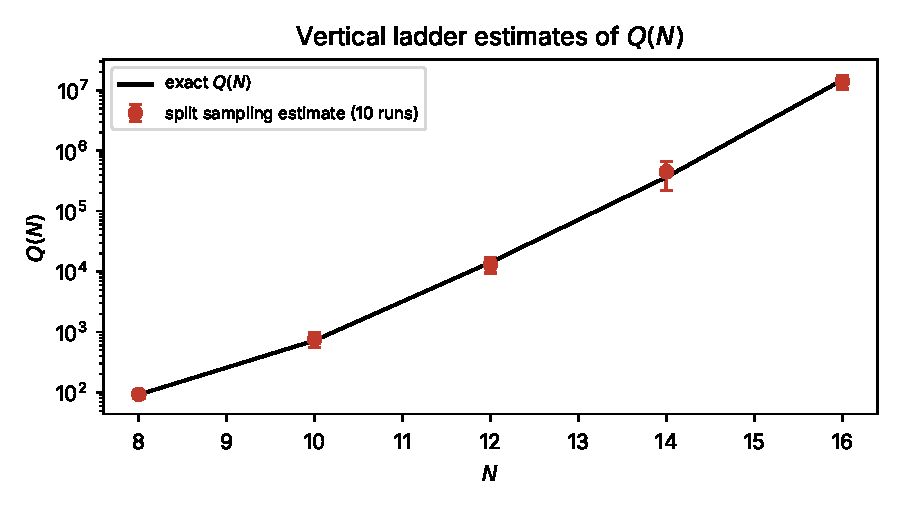
\includegraphics[width=0.9\textwidth]{fig_split.pdf}
\caption{Split sampling estimates of $Q(N)$ with one standard deviation error bars across ten runs, against the exact values.}
\label{fig:split}
\end{figure}

Table~\ref{tab:split} and Figure~\ref{fig:split} give the results. At every $N$ the mean estimate is within a factor $1.25$ of the exact count, and the exact count lies within $0.4$ standard deviations of the mean at every $N$. The coefficient of variation is between $0.13$ and $0.5$, and the ladder has between five and nine rungs. The total cost at $N = 16$ is $9 \times 400 \times 64 \approx 230\,000$ proposed swaps per run, against $16! \approx 2 \times 10^{13}$ permutations to enumerate.

Three observations. First, the number of rungs grows roughly like $N/2$, consistent with the mean energy $2N/3$ of Chapter~\ref{ch:phase} and the geometric decrease of each rung by a factor of about $0.3$ to $0.6$ at the upper rungs, and below $0.3$ over the last two to four rungs. Second, the last two rungs, from energy two to one and from one to zero, have the smallest ratios, and we expect, though we have not measured it per rung, that their level set chains are the slowest. Third, the relative error does not grow visibly with $N$ over this range, which is what one expects if the chain mixes in polynomial time on these level sets at these sizes. Whether it continues not to grow is the mixing conjecture of Chapter~\ref{ch:prp}, and the experiment cannot settle it; it can only say that for $N \le 16$ the walk works.

\section{The ladder}

The ladder from the last of the ten runs at each $N$ is in Table~\ref{tab:ladder}, which lists each level $m_t$ and the estimated ratio $\hat\theta_t = \hat Z_{m_t} / \hat Z_{m_{t-1}}$. Figure~\ref{fig:ladder} plots the cumulative $\log \hat Z_m$ against the level.

\begin{table}[t]
\centering
\small
\caption{The ladder of the last of the ten runs at each $N$: the level $m_t$ and the estimated ratio $\hat\theta_t$ at each rung, read from the top of the ladder down.}
\label{tab:ladder}
\begin{tabular}{rl}
\toprule
$N$ & $(m_t : \hat\theta_t)$ \\
\midrule
8 & $4{:}0.48, \; 3{:}0.54, \; 2{:}0.37, \; 1{:}0.26, \; 0{:}0.12$ \\
10 & $5{:}0.44, \; 4{:}0.63, \; 3{:}0.42, \; 2{:}0.30, \; 1{:}0.12, \; 0{:}0.04$ \\
12 & $6{:}0.39, \; 5{:}0.63, \; 4{:}0.48, \; 3{:}0.34, \; 2{:}0.19, \; 1{:}0.09, \; 0{:}0.04$ \\
14 & $7{:}0.36, \; 5{:}0.32, \; 4{:}0.40, \; 3{:}0.26, \; 2{:}0.16, \; 1{:}0.08, \; 0{:}0.04$ \\
16 & $9{:}0.39, \; 7{:}0.43, \; 6{:}0.48, \; 5{:}0.47, \; 4{:}0.30, \; 3{:}0.21, \; 2{:}0.15, \; 1{:}0.07, \; 0{:}0.01$ \\
\bottomrule
\end{tabular}
\end{table}

\begin{figure}[t]
\centering
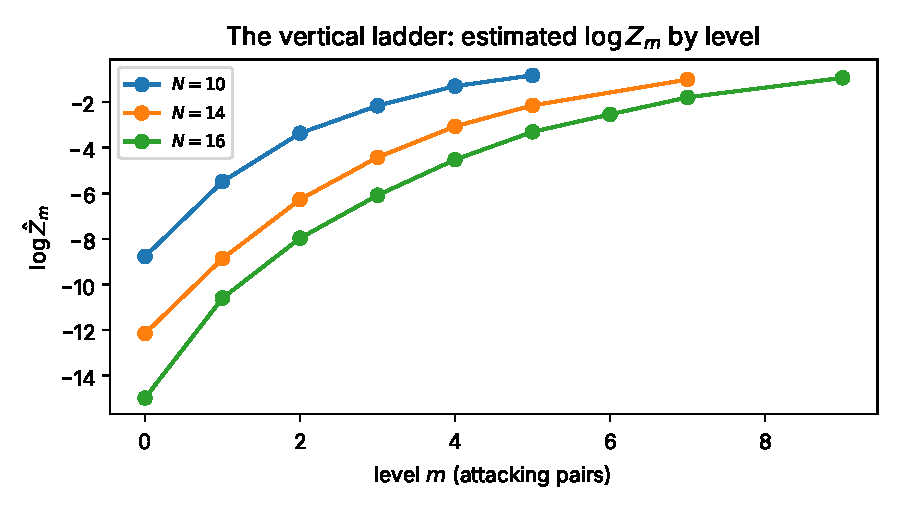
\includegraphics[width=0.9\textwidth]{fig_ladder.pdf}
\caption{Estimated $\log Z_m$ against the level $m$ for $N = 10$, $14$ and $16$, from one run each. The slope steepens as the level approaches zero.}
\label{fig:ladder}
\end{figure}

For $N = 8$ the exact ratios from Table~\ref{tab:dos} are $Z_4 / Z_5 = 0.71$, $Z_3 / Z_4 = 0.58$, $Z_2 / Z_3 = 0.36$, $Z_1 / Z_2 = 0.25$ and $Z_0 / Z_1 = 0.094$. The estimated ladder for $N = 8$ started at level four from the uniform population, where the exact $Z_4 = 0.46$, and its first estimated ratio $0.48$ matches; the subsequent ratios $0.54$, $0.37$, $0.26$ and $0.12$ are close to the exact $0.58$, $0.36$, $0.25$ and $0.094$, as one expects from a population of 400. The ladder is doing what the theory says it should.

The ratios at the bottom of the ladder decrease with $N$: the final ratio $\hat\theta_0 = \hat Z_0 / \hat Z_1$ is $0.12$ at $N = 8$, $0.04$ at $N = 10$ to $14$ and $0.01$ at $N = 16$. This is the steepening of the staircase in the low energy region, a geometric decrease whose limiting behaviour these data do not settle (Chapter~\ref{ch:experiments2} finds the fraction of time at energy zero consistent with decay like $1/N$). The ratio $N(0) / N(1)$ for $N = 8, 9$ from Table~\ref{tab:dos} is $0.104, 0.104$, and the estimated $\hat\theta_0$, which is $N(0) / (N(0) + N(1))$, keeps decreasing at larger $N$, with no limit visible. The final rung is the hardest in two senses at once: its ratio is the smallest, and we expect its chain, confined to permutations with at most one attacking pair, to be the slowest.

\section{Wang Landau and the density of states}

The Wang Landau\index{Wang Landau algorithm} algorithm of Appendix~\ref{app:alg} was run for $N = 10$ with the swap proposal, the flatness criterion that every visited level be visited at least $80\%$ of the mean, and the logarithm of the modification factor halved at each flat histogram. Figure~\ref{fig:wl10} compares the estimated density of states with the exact values from enumeration of the $3\,628\,800$ permutations.

\begin{figure}[t]
\centering
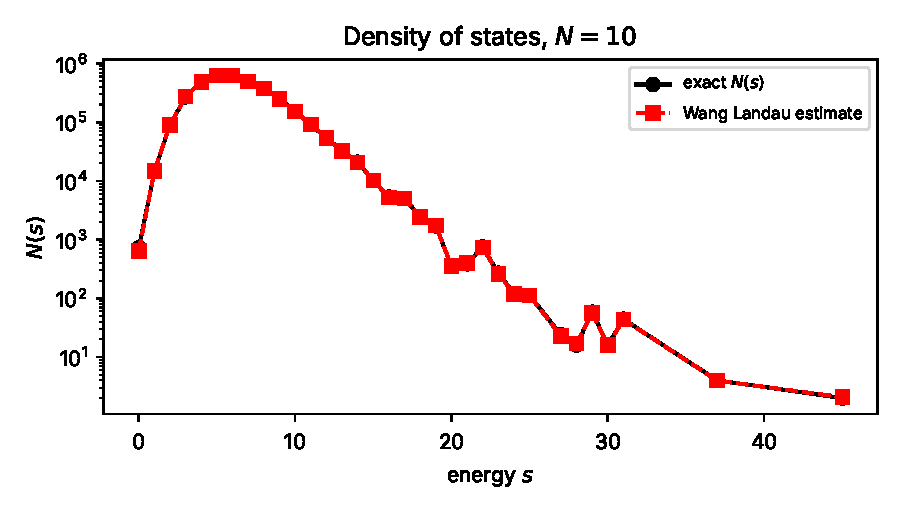
\includegraphics[width=0.9\textwidth]{fig_wl10.pdf}
\caption{Wang Landau estimate of the density of states for $N = 10$ against the exact enumeration, on a logarithmic scale. The estimate is accurate across the bulk and within $12\%$ at the ground state.}
\label{fig:wl10}
\end{figure}

The agreement is close across the bulk, with relative errors below $1\%$ for $s$ from $2$ to $7$ and $3\%$ at $s = 1$, and the ground state estimate is $642$ against the exact $724$, a relative error of $11\%$. The ground state is the hardest level for Wang Landau as it is for the ladder, and for the same reason: the chain reaches it rarely and the few visits give a noisy estimate of its weight. The flat histogram condition forces the chain to spend equal time at every level, which is the $1/N(s)$ reweighting of the multicanonical\index{multicanonical sampler} ensemble, and at the ground state the reweighting is by a factor of $10^3$ relative to the bulk; the chain achieves this by refusing almost every move out of a solution once it finds one, and it finds one rarely.

In the vertical coordinate Wang Landau is estimating all the step widths at once, by visiting them with equal frequency, where the ladder estimates them one at a time from the top. The ladder is more efficient for the ground state because it concentrates its effort there; Wang Landau is more informative because it returns the whole staircase. For counting one wants the ladder; for understanding the structure of the problem one wants Wang Landau, and the staircase it returns for $N = 10$ has 33 nonempty levels, of which the lowest, $s = 0$, carries all $724$ solutions and $0.02\%$ of the permutations.

\section{What the experiments show and do not show}

The experiments show that the vertical ladder is a working algorithm for the queens at the sizes where it can be checked, with a cost that is polynomial by design (a fixed $4N$ swaps per particle per rung) over the range $N \le 16$ and estimates that are unbiased to within sampling error. They show that the difficulty concentrates at the bottom rung, in the size of the ratio, as the theory predicts. And the mixing measurements of Chapter~\ref{ch:experiments2} (Table~\ref{tab:mixing}) suggest that the swap chain on low level sets is slow but not, at these sizes, stuck: the autocorrelation times are between $59$ and $430$ swaps for $N \le 16$.

They do not show that this continues. The mixing conjecture of Chapter~\ref{ch:prp} is about the limit $N \to \infty$, and no experiment at $N = 16$ can speak to it. What an experiment could do is estimate the mixing time\index{mixing time} of the bottom rung chain as a function of $N$ over a wider range, say $N = 8$ to $40$, by running it from many starting solutions and measuring the autocorrelation of some statistic, and look for the onset of exponential growth. We have not done this in this chapter; Chapter~\ref{ch:experiments2} does it for unconditioned boards. On unconditioned boards polynomial growth is what we expect, in line with the conjecture of Chapter~\ref{ch:swendsen}, and the place to look for an exponential is conditioned boards.


\chapter{A Cluster Chain for the Queens}
\label{ch:swendsen}

The swap chain of Chapters~\ref{ch:mixing} and~\ref{ch:experiments} changes two queens at a time and cannot leave a component of a level set that is disconnected under swaps. Cluster chains in the style of Swendsen\index{Swendsen Wang algorithm} and Wang change many variables at once and are a standard tool against the slow mixing that local chains suffer at some phase transitions. This chapter designs such a chain for the queens, proves it is valid, and says what would have to be true for it to mix rapidly.

\section{The queens as a Potts like model}

A permutation $x$ is a perfect matching between rows and columns. The energy $S(x)$ is a sum over pairs of rows,
\[
S(x) = \sum_{i < j} \Ind\{ |x_i - x_j| = j - i \} = \sum_{i < j} J_{ij}(x_i, x_j) ,
\]
a pairwise interaction between the row variables. The Boltzmann\index{Boltzmann distribution} weight $e^{-S/\gamma}$ factors over pairs as $\prod_{i<j} e^{-J_{ij}(x_i, x_j)/\gamma}$, and the hard level set constraint $S \le m$ does not factor but is the limit of a soft one. The structure is that of a Potts model on the complete graph of rows with $N$ colours, the columns, under the constraint that all colours are distinct, which is a hard core exclusion on top of the Potts interaction. The exclusion is what makes the queens a permutation problem and not a spin system.

\section{The Edwards Sokal augmentation}

Write the pairwise weight as $e^{-J_{ij}/\gamma} = (1 - p) + p \, \Ind\{ J_{ij} = 0 \}$ with $p = 1 - e^{-1/\gamma}$, which is valid since $J_{ij} \in \{0, 1\}$. Introduce a bond variable $d_{ij} \in \{0, 1\}$ for each pair with joint weight
\[
w(x, d) = \prod_{i < j} \Big( (1 - p) \, \Ind\{ d_{ij} = 0 \} + p \, \Ind\{ d_{ij} = 1 \} \, \Ind\{ J_{ij}(x_i, x_j) = 0 \} \Big) .
\]
Summing over $d$ recovers the Boltzmann weight of $x$, and the conditional law of $d$ given $x$ is: $d_{ij} = 1$ with probability $p$ if rows $i$ and $j$ do not attack, and $d_{ij} = 0$ otherwise. An open bond $d_{ij} = 1$ records a commitment that rows $i$ and $j$ will not attack after the update.

The conditional law of $x$ given $d$ is uniform over permutations such that every open bond is respected, that is, $|x_i - x_j| \ne j - i$ for all $(i, j)$ with $d_{ij} = 1$, with the unbonded pairs free. This is the Swendsen Wang update, and it is where the queens differ from the Potts model. In the Potts model the constraint of an open bond is that the two spins agree, so the constraint graph decomposes into connected components each of which can be recoloured freely with a single colour, and the update is trivial. For the queens the constraint of an open bond is that the two columns differ by something other than the row distance, which does not reduce to a single colour per component, and sampling a uniform permutation subject to a set of such constraints is itself a hard problem in general.

\section{A tractable cluster move}

The way around this is to restrict which bonds are opened so that the conditional update becomes tractable. Let $R \subseteq \{1, \dots, N\}$ be a random subset of rows, chosen by including each row independently with probability $q$, and open bonds only within $R$ and between $R$ and its complement, with the rows outside $R$ frozen. The update then resamples the columns of the rows in $R$, which is a permutation of the columns they currently occupy, subject to the constraint that the resampled rows do not attack each other along any opened bond and do not attack any frozen row along an opened bond.

For $|R| = 2$ this is the heat bath version of the swap chain. For $|R| = k$ it is a uniform sample from the $k!$ permutations of $k$ columns among $k$ rows subject to diagonal constraints, which for $k$ up to about $8$ can be done by enumeration, and for larger $k$ by a nested swap chain. The resulting algorithm is a block Gibbs sampler that updates a random block of rows at once, and it is valid for the Boltzmann distribution at any temperature by the standard argument, since each step is a Gibbs update of a conditional distribution. For the hard level set $\{ S \le m \}$ we do not take a limit of the Edwards Sokal model, since as $\gamma \to 0$ the Boltzmann law concentrates on minimum energy configurations rather than on the uniform law on the level set. We define the chain directly: choose a random block, and resample it uniformly among block permutations that keep the total energy at most $m$. This is a block Gibbs sampler for the uniform law on $\{ S \le m \}$, which is what the Proposition below needs.

\section{Validity}

\begin{proposition}
\label{prop:blockvalid}
The block chain with binomially distributed block size and exact resampling of each block conditional on the level set is reversible with respect to the uniform distribution on the level set, and is irreducible on it whenever the level set is connected under moves that permute any $k$ rows at once for $k$ up to the maximal block size attained.
\end{proposition}

\begin{proof}
Each step is a Gibbs update of the conditional distribution of the block given the rest, which is reversible with respect to the target. The chain is a mixture over blocks of reversible kernels and is reversible. Irreducibility is by definition of connectivity under the allowed moves.
\end{proof}

The chain is therefore valid, and the question is its mixing time\index{mixing time}. With $q = 2/N$ it is essentially the swap chain. With $q = 1$ it resamples the whole board exactly, which is the problem itself. The interesting regime is $q$ a constant such as $1/4$, where each step moves a quarter of the queens and the block resampling is done by a nested chain, which the Proposition covers only if it is reversible for the block conditional.

\section{What rapid mixing would require}

For the block chain to mix rapidly on $\{ S \le 1 \}$ at constant block fraction $q$, two things are needed. The level set must be connected under block moves, which is weaker than connectivity under swaps and is plausible: any two solutions differ in some set of rows, and if that set is at most $qN$ a single block move connects them. And the conductance\index{conductance} must be inverse polynomial, which means that from any subset of the level set of mass at most a half, a block move escapes with probability at least $1/\mathrm{poly}(N)$. The second is the hard part. If the level set has exponentially many components under swaps, each polynomial in size, then escape from a component requires that the exact block conditional given the frozen rows put appreciable mass outside the current component. We expect, without proof, that for a typical block the frozen rows leave few completions of energy at most $1$, so that the conditional is concentrated on the current configuration and a few neighbours, and then the conductance is exponentially small.

This is the same obstruction as before at a coarser scale. The cluster chain enlarges the neighbourhood of a configuration from $\binom{N}{2}$ swaps to $\binom{N}{qN} (qN)!$ block permutations, but if the solutions are spread uniformly over an exponentially larger space the enlargement does not help: the fraction of the neighbourhood that consists of solutions is still exponentially small (a heuristic about proposals; for the exact block update the relevant statement is the one above about the block conditional). Cluster chains defeat phase transitions in the Potts model because the clusters are correlated with the structure of the low energy states, the magnetised domains, and a cluster move flips a domain. For the queens there is no analogue of a domain that we can see, and the block moves are not correlated with anything.

\section{A conjecture and an experiment}

\begin{conjecture}
\label{conj:blockmix}
For the block chain on $\{ S \le 1 \}$ for the unconditioned $N$ queens problem, the mixing time is polynomial in $N$ for every constant $q \in (0, 1)$. For the block chain on $\{ S \le 1 \}$ for the completion problem with partial placements drawn from the Gent Jefferson Nightingale~\cite{GJN} reduction applied to hard satisfiability instances, the mixing time is superpolynomial for every $q$ bounded away from one.
\end{conjecture}

The first half says that the unconditioned problem, which is in $\Pc$ as a decision problem and which the experiments of Chapter~\ref{ch:experiments2} suggest is well behaved, has well connected level sets. The second half says that the conditioning, which is where the $\NP$ hardness enters, shatters them. The experiment that tests both is to run the block chain on unconditioned and on reduction boards for $N$ up to $40$, measure autocorrelation times and genealogical coalescence, and compare. We have run it only for the swap chain and only on unconditioned boards, and we report the results in the next chapter. The conditioned case is the one that matters, and it is open.


\chapter{Numerical Experiments II: The Bottom Rung}
\label{ch:experiments2}

Chapter~\ref{ch:experiments} ended by describing the experiment it had not done: the mixing time\index{mixing time} of the bottom rung chain as a function of $N$. This chapter does it for the swap chain on unconditioned boards up to $N = 32$. The result is that the autocorrelation time grows like $N^{1.8}$ over this range, which is polynomial, and the ratio $Z_0 / Z_1$ estimated from the chain decreases roughly like $0.5/N$ over this range, so that the data do not show a positive limit. On unconditioned boards, at these sizes, the bottom rung is not stuck.

\section{Design}

For each $N$ in $\{ 8, 10, 12, 14, 16, 18, 20, 24, 28, 32 \}$ a solution was found by a min conflicts heuristic, and the swap chain on $\{ S \le 1 \}$ was run from it for $4000 N$ proposed swaps, recording at each step the column $x_1$ of the queen in the first row. The integrated autocorrelation time of this sequence,
\[
\tau_{\rm int} = 1 + 2 \sum_{k \ge 1} \mathrm{corr}(x_1(t), x_1(t + k)) ,
\]
was estimated with the sum truncated where the correlation first falls below $0.02$. The statistic $x_1$ was chosen because it is a coordinate of the configuration that must be decorrelated for the chain to have mixed, and because it is cheap; the column of any row would do. Six independent runs from six independent starting solutions were made at each $N$ and the mean and standard deviation of $\tau_{\rm int}$ recorded. A separate run of $2000 N$ steps recorded the fraction of time the chain spent at energy zero, which estimates $Z_0 / Z_1 = N(0) / (N(0) + N(1))$.

\section{Results}

\begin{table}[t]
\centering
\small
\caption{Integrated autocorrelation time of the first row column under the swap chain on $\{ S \le 1 \}$, in proposed swaps, mean and standard deviation over six runs; and the fraction of time at energy zero.}
\label{tab:mixing}
\begin{tabular}{rrrr}
\toprule
$N$ & $\tau_{\rm int}$ mean & $\tau_{\rm int}$ sd & fraction at $S = 0$ \\
\midrule
8 & 59 & 10 & 0.094 \\
10 & 168 & 31 & 0.061 \\
12 & 297 & 82 & 0.034 \\
14 & 423 & 128 & 0.044 \\
16 & 430 & 166 & 0.032 \\
18 & 398 & 29 & 0.023 \\
20 & 528 & 62 & 0.022 \\
24 & 994 & 544 & 0.019 \\
28 & 723 & 169 & 0.014 \\
32 & 928 & 101 & 0.018 \\
\bottomrule
\end{tabular}
\end{table}

\begin{figure}[t]
\centering
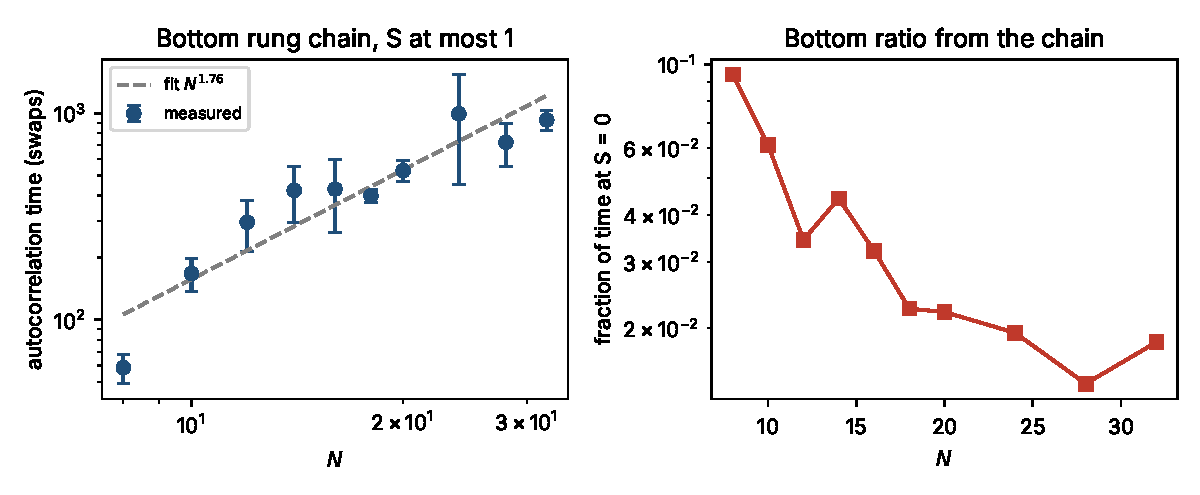
\includegraphics[width=\textwidth]{fig_mixing.pdf}
\caption{Left: autocorrelation time of the bottom rung chain against $N$ on logarithmic axes, with a power law fit of exponent $1.76$. Right: the fraction of time at energy zero, which estimates $Z_0 / Z_1$.}
\label{fig:mixing}
\end{figure}

Table~\ref{tab:mixing} and Figure~\ref{fig:mixing} give the results. The autocorrelation time grows from $59$ swaps at $N = 8$ to about $900$ at $N = 32$, and a power law fit on logarithmic axes gives an exponent of $1.76$ with no clear curvature given the scatter. The fraction of time at energy zero, which is the bottom ratio of the ladder, falls from $0.094$ at $N = 8$, where the exact value is $92 / (92 + 888) = 0.094$, to about $0.015$ at $N = 28$ to $32$, and its product with $N$ stays between $0.4$ and $0.75$, so the decrease is consistent with decay like $1/N$ and the data do not show a positive limit.

\section{Interpretation}

Three readings.

First, the swap chain on $\{ S \le 1 \}$ for unconditioned boards does mix, in the sense that the first row column decorrelates in a number of steps polynomial in $N$ over the range tested. Since each proposed swap costs $O(N)$ to evaluate incrementally, the cost of an effectively independent sample is $O(N^{2.8})$, and the cost of the bottom rung of the ladder with $M$ samples is $O(M N^{2.8})$. With $M = O(N / \epsilon^2)$, which assumes the bottom ratio is bounded below and which the data above do not show, from the product estimator\index{product estimator} bound this is $O(N^{3.8} / \epsilon^2)$ for the bottom rung, and the whole ladder is $O(N)$ rungs each cheaper than the bottom, so the walk on unconditioned boards costs $O(N^{4.8} / \epsilon^2)$ if the exponent holds. This is an extrapolated cost estimate, not a demonstrated polynomial algorithm: the counts were checked against exact values only to $N = 16$, the exponent is measured on a finite range, and the estimate assumes that the upper rungs are cheaper than the bottom one. The relaxation times of Chapter~\ref{ch:open} grow faster, like $N^3$, which would raise the exponent.

Second, this says nothing about the completion problem on hard instances, which is where the $\NP$ hardness is. The unconditioned level set $\{ S \le 1 \}$ contains all $Q(N)$ solutions together with the $N(1)$ placements with one attacking pair, and since $Q(N)$ grows like $N!$ times $e^{-0.942 N}$ up to subexponential factors there are a great many solutions, spread through the permutation group, and the one attack placements serve as bridges between them. On a conditioned board with few free rows, or on a reduction board where the free squares are a sparse pattern designed to encode a formula, the level set is small and its connectivity under swaps is a different question entirely. The experiment is consistent with the first half of the conjecture of Chapter~\ref{ch:swendsen}, though it concerns the swap chain and not the block chain. The exact connectivity computations of Chapter~\ref{ch:open} extend the support to boards conditioned on queens of a random solution, up to $N = 17$, where the giant component\index{giant component} of completions survives; they are silent on adversarially conditioned boards.

Third, the ratio $Z_0 / Z_1$ decreases slowly with $N$, and the data do not settle whether the number of placements with exactly one attacking pair is a bounded multiple of the number of solutions: the implied ratio $N(1)/N(0)$ rises from about $10$ at $N = 8$ to roughly $50$ to $70$ at the largest $N$, with no sign of saturating. This is a statement about the solution landscape: on average a solution is surrounded by a polynomial number of near solutions, which is why the swap chain can move, and it suggests that the bottom rung could be replaced by a direct count of near solutions per solution if that multiple could be computed. We leave this as an open problem.

\section{What would change the picture}

A further experiment would sharpen the picture considerably, and it is within reach of a laptop.

Run the same chain on reduction boards. Take a small hard satisfiability instance, apply the Gent Jefferson Nightingale~\cite{GJN} construction to obtain a board and a partial placement, and run the swap chain on the level set $\{ S \le 1 \}$ of the free rows. If the autocorrelation time explodes, or the chain fails to leave the component it starts in, the second half of the conjecture is supported. The construction is intricate and we have not implemented it; doing so is the most valuable next step in the program.

\section{Summary}

On unconditioned boards the bottom rung autocorrelation time grows like $N^{1.8}$ up to $N = 32$, which under the assumptions above extrapolates to a cost near $N^5$ for the vertical walk; the counts themselves were checked against exact values only to $N = 16$. This is the first measurement of the mixing of the queens level set chain that we know of, and it suggests that for the unconditioned problem the Monte Carlo program works at these sizes. For the completion problem on hard boards, which is the problem whose solution in randomized polynomial time would give $\NP = \RP$, we have no measurement. What we have, from the exact computations of Chapter~\ref{ch:open}, is the measurement on boards conditioned on randomly placed queens at $N = 12$, a pointer rather than a result: the bottom level set appears to shatter there, so that the chain of this chapter would be trapped, but the level set three or four attacks up is connected, so that the walk with the bottom rungs skipped would not be. On random boards the typical depth has since been measured to move by about one, from 3 at $N = 12$ to 4 at $N = 16$, which the data do not yet show to be growth (Section~\ref{sec:round4} of Chapter~\ref{ch:open}). The question for hard boards is whether the depth stays bounded or grows with $N$, and we expect, when that measurement is made, that it grows.


\chapter{Numerical Experiments III: Genealogies}
\label{ch:genealogy}

Chapter~\ref{ch:smc} proposed the genealogy of the particle system as the diagnostic for shattered level sets, and Chapter~\ref{ch:witchhat} argued that it is a chain based diagnostic that can see something a single chain cannot. This chapter runs it. For the unconditioned queens at $N = 10, 14, 18$ and $22$ and for randomly conditioned boards at $N = 14$ and $18$, we record at each rung of the ladder the number of distinct initial ancestors of the surviving particles, and compare with the number predicted by a neutral model in which selection alone, with no structure in the level set, causes the coalescence. The two agree closely, with two exceptions noted below. On these boards the genealogy shows little coalescence beyond that of selection, which is what connected level sets and rapid mixing would produce, though at this resolution it does not prove them.

\section{The neutral model}

The split sampler of Chapter~\ref{ch:experiments} keeps $M$ particles, selects at each rung the fraction $f_t$ with energy at or below the new level, and refills the population by copying the elite cyclically and mutating each copy by the level set chain. Label each initial particle with an ancestor index and carry the index through selection and mutation. After rung $t$ let $A_t$ be the number of distinct ancestors among the elite.

If the level set at rung $t$ is connected and the chain mixes within it, the energies of the particles at the next selection are independent of their ancestry, and selection of a fraction $f_{t+1}$ picks a random subset. With $A_t$ ancestors each represented by about $M / A_t$ particles, the expected number of ancestors that survive a random selection of fraction $f_{t+1}$ is
\[
A_{t+1} \approx A_t \big( 1 - (1 - f_{t+1})^{M / A_t} \big) ,
\]
which is the neutral prediction. If instead the level set has shattered into components and the particles of some ancestors are in components from which the next level is unreachable, those ancestors are lost in a block, and $A_{t+1}$ falls below the neutral prediction. A coalescence to one ancestor at the bottom rung, where the neutral model predicts several, would be the signature of the mixing conjecture's failure.

\section{Results}

Table~\ref{tab:genealogy} gives, for each run, the level $m_t$, the observed $A_t$ and the neutral prediction, rung by rung down to the solutions. The prediction iterates the recursion above from $A_0 = M$ on its own predicted values, using the observed selected fractions, rather than applying it to the observed $A_t$ at each rung. The equal family size formula is an upper bound on the neutral expectation, since $1 - (1-f)^n$ is concave in $n$ and cyclic copying leaves family sizes unequal, so a shortfall of the observed count below the prediction is expected even under neutrality; the comparison therefore cannot separate structure from this bias. The predicted counts of the table are a hand computation from the recursion above and the observed fractions in code/genealogy.json; no script in the code directory computes them.

\begin{table}[t]
\centering
\footnotesize
\caption{\footnotesize Distinct ancestors among the elite at each rung, observed against the neutral prediction, for $M = 400$ particles. Unconditioned boards at $N = 10, 14, 18, 22$ and randomly conditioned boards with $k$ queens of a solution fixed. Each cell is level: observed / predicted.}
\label{tab:genealogy}
\begin{tabular}{lp{4.3in}}
\toprule
board & ancestors by rung (level: observed / predicted) \\
\midrule
$N = 10$ & $5{:}167/167, \; 4{:}142/142, \; 3{:}111/120, \; 2{:}75/80, \; 1{:}38/42, \; 0{:}11/12$ \\
$N = 14$ & $7{:}134/134, \; 6{:}124/125, \; 5{:}101/113, \; 4{:}84/94, \; 3{:}54/68,$ \\
 & $2{:}39/43, \; 1{:}25/24, \; 0{:}7/7$ \\
$N = 18$ & $10{:}162/162, \; 8{:}114/118, \; 7{:}101/110, \; 6{:}87/99, \; 5{:}71/81,$ \\
 & $4{:}54/63, \; 3{:}42/49, \; 2{:}25/28, \; 1{:}10/13, \; 0{:}4/8$ \\
$N = 22$ & $12{:}131/131, \; 10{:}107/109, \; 9{:}100/102, \; 8{:}94/96, \; 7{:}72/82,$ \\
 & $6{:}57/74, \; 5{:}40/53, \; 4{:}32/39, \; 3{:}21/27, \; 2{:}15/20, \; 1{:}12/12, \; 0{:}6/6$ \\
$N = 14$, $k = 3$ & $7{:}142/142, \; 5{:}88/90, \; 4{:}76/79, \; 3{:}57/65, \; 2{:}41/47,$ \\
 & $1{:}23/27, \; 0{:}13/19$ \\
$N = 18$, $k = 5$ & $8{:}134/134, \; 7{:}122/125, \; 6{:}104/113, \; 5{:}84/93, \; 4{:}60/72,$ \\
 & $3{:}43/52, \; 2{:}26/33, \; 1{:}16/19, \; 0{:}6/7$ \\
\bottomrule
\end{tabular}
\end{table}

Three observations. First, the observed ancestor counts track the neutral prediction at every rung on every board, up to a one sided shortfall, since in 41 of the 52 cells the observed count is below the prediction, 10 are equal and one is above, and we have no replicate runs to measure the fluctuation: the typical shortfall is $10$ to $20\%$ in the middle rungs and the bottom rung counts agree to within one or two except at $N = 18$ ($4$ against $8$) and at $N = 14$, $k = 3$ ($13$ against $19$). The $N = 18$ bottom rung loses half the predicted ancestors, which is the size of block loss that a diagnostic should detect, so we cannot say that there is no block loss of ancestors; at this particle number we cannot tell it from a fluctuation. Second, the coalescence is severe in absolute terms, from $400$ ancestors to between $4$ and $13$ at the bottom, but it is the coalescence of selection, not of structure: with selected fractions between $0.02$ and $0.60$ over six to twelve rungs, a neutral population loses most of its ancestry, and this is what happens. Third, the conditioned boards behave like the unconditioned ones, consistent with the exact connectivity computations of Chapter~\ref{ch:open}.

\section{Interpretation}

The genealogy is consistent with the first half of the mixing conjecture, within the bias noted above and the resolution limits discussed below. A single chain's autocorrelation time, measured in Chapter~\ref{ch:experiments2}, says that the chain moves within whatever it can reach; the genealogy says that what the population reaches at the bottom is reached from many independent starting points in proportion to their share of the population, which is what connectedness would produce, though the comparison cannot separate this from the bias noted above. The witch's hat of Chapter~\ref{ch:witchhat} would show up here as a population that, starting from $400$ dispersed points, arrives at the spike from only one or two of them while the neutral model predicts ten; nothing of the kind appears.

The experiment also tells us how to size the particle system. The neutral ancestry at the bottom scales roughly linearly in $M$: iterating the neutral recursion with the observed fractions, $M = 400$ leaves between $6$ and $19$ ancestors and $M = 4000$ would leave between $59$ and $187$. A diagnostic that aims to detect a block loss of, say, half the ancestors needs the neutral count at the bottom to be well above ten, which means $M$ in the thousands for $N$ above $20$. The resampling scheme matters as well: cyclic copying of the elite, which we used, preserves ancestry evenly, whereas multinomial resampling adds its own coalescence and would blur the signal.

\section{The experiment on hard boards}

The experiment that remains is the same one that has remained throughout: the genealogy on reduction boards. There the prediction is the opposite of what Table~\ref{tab:genealogy} shows. A board encoding a hard formula has, if the picture of Chapter~\ref{ch:ogp} is right, completions in exponentially many components with the overlap gap property, and a particle population descending the ladder will find, at the bottom rung, that the particles in most components cannot reach a completion at all, since their near completions are near completions of an unsatisfying assignment and the level set below is empty for them. The ancestry at the bottom will collapse to those few initial particles, if any, that happened to start in the basin of a satisfying cluster, and the neutral model will overpredict by a large factor. That collapse, measured against the neutral prediction, would be the first direct Monte Carlo observation of the mechanism that the whole program says must be there. It needs the reduction implemented, and Chapter~\ref{ch:experiments2} says why we have not done it; it is the next thing to do.

\section{Summary of the three experiments}

The three experimental chapters now say the following. The ladder counts the unconditioned queens correctly to $N = 16$, at a cost that has been measured only up to that size; polynomial scaling is extrapolated. The bottom rung chain has autocorrelation time growing like $N^{1.8}$ to $N = 32$. The genealogy shows coalescence close to neutral, which is consistent with connected level sets, to $N = 22$ unconditioned and $N = 18$ randomly conditioned; at $M = 400$ the bottom predictions are only 6 to 19 ancestors, so it cannot exclude a block loss of half, and the mixing of the chain between rungs, run for a few sweeps, is assumed rather than tested. Together with the exact giant component computations to $N = 17$, the evidence that the Monte Carlo program works on boards that encode nothing is suggestive. The evidence that it fails on boards that encode something is, as yet, the consensus of complexity theory and the overlap gap theorems for the problems the boards would encode, and no measurement of our own.


\chapter{Other Laboratories}
\label{ch:labs}

The queens are one hard counting problem among many, and the vertical view applies to all of them. This chapter runs through five others, the permanent, the Ising model, the volume of a convex body, satisfying assignments, and the number of linear extensions of a partial order, and for each describes the staircase, the level set sampler\index{level set sampler}, and the status of mixing. The pattern that emerges is uniform: in these five cases the problems for which the walk is known to be polynomial are exactly those whose decision versions are easy, and for every one of them the staircase has the same shape.

\section{The permanent}

For an $n \times n$ zero one matrix $A$ the permanent $\mathrm{per}(A) = \sum_\sigma \prod_i A_{i, \sigma(i)}$ counts the perfect matchings of the bipartite graph with adjacency matrix $A$. It is $\sharpP$ complete by Valiant\index{Valiant, Leslie}, and the existence of a perfect matching is in $\Pc$ by Edmonds\index{Edmonds, Jack}, and in $\RP$ by the determinant of the Edmonds matrix. The natural energy on permutations is $S(\sigma) = \#\{ i : A_{i, \sigma(i)} = 0 \}$, the number of non edges used, and the permanent is $N(0)$. The staircase has at most $n + 1$ steps.

Jerrum and Sinclair's 1989 algorithm runs a chain on matchings, not permutations, that adds or removes an edge or shifts an endpoint, and is reversible with respect to a distribution that weights matchings by a factor $\lambda^{\text{number of edges}}$; the ratio of perfect to near perfect matchings is estimated at a sequence of $\lambda$ values, which is an annealing\index{simulated annealing} ladder in $\lambda$. For dense matrices, with every row and column sum at least $n/2$, the chain mixes in polynomial time by canonical paths. Jerrum, Sinclair and Vigoda in 2004 handled arbitrary nonnegative matrices by weighting the near perfect matchings according to which vertices they miss, with the weights learned adaptively in a manner that resembles Wang Landau\index{Wang Landau algorithm}. The result is an FPRAS of running time $O^*(n^{10})$, later improved to $O^*(n^7)$ by Bez\'akov\'a, \v{S}tefankovi\v{c}, Vazirani and Vigoda using an improved cooling schedule.

The vertical reading: the ladder in $\lambda$ is a sequence of tilts of the staircase, and the adaptive weights of Jerrum, Sinclair and Vigoda are the flat histogram condition applied to the hole positions. The permanent\index{permanent} is the showcase for the thesis in the easy direction. Its decision problem is in $\Pc$, its staircase is short, its level sets are connected under local moves with polynomial congestion, and the walk is polynomial.

\section{The Ising model}

The ferromagnetic Ising model on a graph $G$ has configurations $\sigma \in \{\pm 1\}^V$, energy $H(\sigma) = -\sum_{(i,j) \in E} \sigma_i \sigma_j$, and partition function $Z(\beta) = \sum_\sigma e^{-\beta H(\sigma)}$. Computing $Z$ is $\sharpP$ complete even for planar graphs with a magnetic field, by Jerrum and Sinclair, and counting the ground states is the number of minimum cuts, which is in $\Pc$. The staircase has at most $|E| + 1$ steps indexed by the number of unsatisfied edges.

Jerrum and Sinclair gave an FPRAS\index{FPRAS} for $Z(\beta)$ at all $\beta$ in the ferromagnetic case, by running a chain not on spins but on the subgraphs of the high temperature expansion, which have no phase transition. Glauber dynamics mixes rapidly above the critical temperature and torpid\index{torpid mixing}ly below it on lattices, by the bottleneck between the two magnetised phases, while Swendsen\index{Swendsen Wang algorithm} Wang mixes rapidly for the Ising model on every graph at every temperature by Guo and Jerrum (2018); torpid mixing of Swendsen Wang is a Potts phenomenon, shown on the complete graph at criticality for $q \ge 3$ by Gore and Jerrum. The hard core model of independent sets is hard to approximate beyond the uniqueness threshold in the fugacity, by Sly's theorem of 2010, and the antiferromagnetic Ising model beyond its uniqueness threshold by Sly and Sun (2012); with Weitz's algorithm (2006) below the threshold this shows that the computational threshold coincides with the uniqueness threshold on the infinite regular tree.

The vertical reading: the staircase of the Ising model is smooth and well behaved, but its level sets are disconnected under spin flips below the critical temperature, which is the physical phase transition, and the walk needs the cluster or subgraph chains to get through. Sly's theorem is the sharpest known statement that a physical transition can be a computational one: on the hard side the staircase cannot be climbed, by any method, unless $\NP = \RP$.

\section{The volume of a convex body}

For a convex body $K \subseteq \mathbb{R}^n$ given by a membership oracle, the volume is $\sharpP$ hard to compute exactly and, by B\'ar\'any and F\"uredi, cannot be approximated by any deterministic polynomial time algorithm to within a factor better than $(cn / \log n)^{n/2}$. Dyer, Frieze and Kannan\index{Dyer, Frieze and Kannan} showed in 1991 that it can be approximated by a randomized algorithm, the first instance of a provable exponential gap between deterministic and randomized approximation. The algorithm is a ladder: a sequence of bodies $K_0 \subseteq K_1 \subseteq \dots \subseteq K_T = K$, with $K_0$ a ball of known volume and each $K_{i+1}$ at most a constant factor larger than $K_i$, and the ratios $\mathrm{vol}(K_i) / \mathrm{vol}(K_{i+1})$ estimated by sampling from $K_{i+1}$ with a random walk. The original running time $O^*(n^{23})$ has been reduced over thirty years to $O^*(n^4)$ by Lov\'asz\index{Lov\'asz, L\'aszl\'o} and Vempala and to $O^*(n^3)$ by Cousins and Vempala, through better walks, better isoperimetric inequalities, and better ladders, including the Gaussian cooling ladder of Cousins and Vempala in which $K_i$ is replaced by a Gauss\index{Gauss, Carl Friedrich}ian weighting of $K$ at inverse temperature $\beta_i$.

The vertical reading is exact. The likelihood is $L(x) = \Ind_K(x)$ under a Gaussian or uniform reference, the quantile function is a single step of width $\mathrm{vol}(K) / \mathrm{vol}(\text{reference})$, and the annealing ladder in $\beta$ is a sequence of tilts that walks the step from near one to its true position. The walk is polynomial because the level sets, which are convex bodies, are connected and have conductance bounded by the isoperimetric constant of a convex body, which Kannan, Lov\'asz and Simonovits showed is at least inverse polynomial. Applegate\index{Applegate, Kannan and Polson}, Kannan and Polson, and then Frieze, Kannan and Polson with the Metropolis\index{Metropolis algorithm} ball walk, extended the random walk and its analysis from indicators of convex bodies to log concave functions, which is the Bayesian case: a posterior proportional to a log concave likelihood times a log concave prior is sampled and integrated by the same walk, and the vertical ladder for its evidence has the same polynomial guarantee. This is a point at which Bayesian computation and complexity theory touched, and it is no accident that it was through a volume.

\section{Satisfying assignments}

For a Boolean formula $\varphi$ in conjunctive normal form, the number of satisfying assignments $\#\mathrm{SAT}$ is $\sharpP$ complete and the decision problem is $\NP$ complete. The natural energy is the number of unsatisfied clauses, and the staircase has at most $m + 1$ steps for $m$ clauses. A level set sampler would be a chain on assignments with at most $k$ unsatisfied clauses; WalkSAT and its relatives are such chains, used as optimisers rather than samplers, and their empirical success on random instances below the satisfiability threshold and failure above it is the heuristic form of a phase transition. The picture from the statistical physics of random constraint satisfaction, is that the solution space of a random $k$ SAT instance shatters into exponentially many clusters at a clause density below the satisfiability threshold, the clustering transition, and that local chains cannot move between clusters. This is the mechanism we conjectured for the queens in Chapter~\ref{ch:phase}, and in the random SAT setting with $k$ large enough it is established at the level of rigorous theorems by Achlioptas, Coja Oghlan and others.

The vertical reading: the staircase of $\#\mathrm{SAT}$ is short and the walk needs $O(m)$ rungs, but the bottom rungs are level sets that shatter into exponentially many components, and no local chain mixes across them. The clustering transition is the mixing conjecture made concrete, and it is a theorem for random instances with $k$ large enough.

\section{Linear extensions}

A partial order on $n$ elements has some number of linear extensions, the total orders compatible with it, and Brightwell and Winkler showed in 1991 that counting them is $\sharpP$ complete. Finding one is trivial by topological sort. The problem is self reducible\index{self reducibility} and the level sets are connected: the linear extensions index the simplices of volume $1/n!$ in the canonical triangulation of the order polytope, and a chain that swaps adjacent elements when the swap respects the order mixes in polynomial time by a coupling\index{coupling} argument due to Bubley and Dyer, with mixing time $O(n^3 \log n)$. The count therefore has an FPRAS, and indeed the volume of the order polytope, which is the count divided by $n!$, can also be approximated by the convex body algorithm.

The vertical reading: the energy is the number of order violations, the ground step is the set of linear extensions, and the walk is polynomial because the adjacent transposition chain on the ground step itself mixes rapidly. This is a case where the bottom rung, which for the queens is the hardest, is directly samplable, and the ladder is not needed; the count can be obtained by the Jerrum Valiant Vazirani self reducibility route from a uniform sampler on the ground step alone.

\section{The pattern}

Set the five problems and the queens side by side.

The permanent, the ferromagnetic Ising model, the volume and linear extensions have decision versions in $\Pc$, staircases of polynomial length, and level sets whose connectivity and conductance\index{conductance} can be bounded (for the Ising model by the cluster or subgraph chains and not by spin flips), and the walk is polynomial for all of them. Satisfying assignments and the queens completion have $\NP$ complete decision versions, staircases of polynomial length, and level sets that are believed, and for random $k$ SAT with $k$ large proved, to shatter at low energy, and the walk is believed to be exponential for both.

The staircase itself is never the obstruction. In every case it has polynomially many steps, and in every case the quantile reordering reduces the exponential sum to a polynomial sum of widths. The obstruction, when there is one, is always the bottom rungs, and always for the same reason: the level sets fall apart into pieces that no efficiently implementable chain can connect. The thesis of this book is that this pattern is not a coincidence but the content of $\NP \neq \RP$ seen from the quantile axis. The same axis, with a single step, is where $\Pc = \RP$ lives, and the question there is whether the single bottom rung, which has density at least a half, can be hit without a chain at all.


\chapter{Average Case Hardness and the Overlap Gap Property}
\label{ch:ogp}

The $\NP$ completeness of the queens completion problem is a worst case statement. The experiments and exact computations of this book are on random instances, unconditioned boards or boards conditioned on queens of a solution, and they find the chain working. The gap between worst case and average case is the subject of a theory of its own, and in the last decade that theory has produced a precise geometric criterion, the overlap gap property, for when stable algorithms, local algorithms among them, must fail on random instances. This chapter presents the criterion and asks whether the queens have it.

\section{Levin's average case completeness}

Levin defined in 1986 a distributional problem as a pair of a language and a polynomial time computable distribution on instances, and showed that there are distributional problems complete for the class of all $\NP$ problems with computable distributions (extended to samplable distributions by Impagliazzo and Levin in 1990): if any one of them is solvable in polynomial time on average, all are. The theory is the formal home of Impagliazzo's Heuristica, the world in which $\NP$ problems are hard in the worst case and easy on average, and the distinction between that world and Pessiland is whether average case hard problems exist. Levin's complete problems are artificial, tiling problems with carefully chosen distributions, and the question of whether natural problems such as random satisfiability or random queens completion are hard on average is open and is attacked by different means.

\section{Random satisfiability and the clustering transition}

The natural setting is random $k$ SAT: $n$ variables, $m = \alpha n$ clauses each a random $k$ tuple of literals. For $k = 3$ the formula is believed to be satisfiable with high probability for $\alpha$ below a threshold near $4.27$ and unsatisfiable above it, by the sharp threshold theorem of Friedgut and the numerical and physical determination of the threshold by M\'ezard, Parisi and Zecchina and its rigorous confirmation for large $k$ by Ding, Sly and Sun in 2015. Below the threshold the solutions exist and the question is whether they can be found.

The statistical physics of the problem, through the cavity method, predicts a sequence of transitions in the geometry of the solution space as $\alpha$ increases: a clustering transition at which the solutions, previously a single connected set under single variable flips, shatter into exponentially many clusters separated by Hamming distance linear in $n$; a condensation transition at which a bounded number of clusters carry most of the solutions; and a freezing transition at which most variables in a typical cluster are fixed. Achlioptas and Coja Oghlan proved the clustering transition rigorously in 2008 for $k$ large enough, and for large $k$ the algorithmic barrier is observed near there: every known polynomial time algorithm finds solutions only below about the clustering density, which is near $2^k \log k / k$, a factor of order $k / \log k$ below the satisfiability threshold near $2^k \log 2$.

In the vocabulary of this book the clustering transition is the shattering of the bottom level set. Below it the solutions are predicted to form one giant component in which a local chain mixes; above it they are exponentially many components of exponentially small relative size, and no local chain crosses between them.

\section{The overlap gap property}

Gamarnik and Sudan in 2014, and Gamarnik with Jagannath, Wein and others since, turned the clustering picture into a proof technique. A problem has the overlap gap property, OGP, if there are constants $0 < \nu_1 < \nu_2 < 1$ such that, with high probability over the random instance, every pair of near optimal solutions has normalised overlap either less than $\nu_1$ or greater than $\nu_2$: there are no pairs at intermediate overlap. The property says that the solution space is clustered with a gap, in the sense that two solutions are either in the same cluster or far apart, with nothing in between.

The theorem is that OGP rules out stable algorithms. An algorithm is stable if a small change in the instance produces a small change in the output; local algorithms, low degree polynomials of the instance, approximate message passing, and Langevin dynamics run for bounded time are all stable in the appropriate sense. The argument interpolates between two instances, shows that a stable algorithm's outputs on the interpolated instances move continuously in overlap, and derives a contradiction from the gap. Gamarnik and Sudan applied it to independent sets in sparse random graphs, Gamarnik and Jagannath to the spin glass ground state, Gamarnik and Sudan and Bresler and Huang to random $k$ SAT variants, and Gamarnik and Zadik, and Wein and coauthors, to planted problems. In several cases the OGP threshold is close to the empirically observed algorithmic threshold, though not in all, and for independent sets the gap was closed only by later multi overlap arguments. For the spin glass, the absence of OGP is conjectured for the SK model and is the hypothesis under which Montanari's algorithm succeeds, and Huang and Sellke showed the matching hardness at the algorithmic threshold.

OGP is the first general tool that proves average case hardness for a natural class of algorithms without any complexity assumption, and whether the class includes the chains of this book is not known: polynomial time Markov chains are not among the algorithms for which stability has been proved. It does not prove $\Pc \neq \NP$ or anything about worst case; it proves that on random instances past the threshold, stable algorithms do not reach the optimum.

\section{Do the queens have the overlap gap property?}

Define the overlap of two queens solutions as the fraction of rows on which they agree. The question is whether, for the uniform distribution on solutions of the unconditioned problem or on completions of a randomly conditioned board, the pairwise overlaps show a gap.

For the unconditioned problem the exact computations of Chapter~\ref{ch:open} say no at small $N$: the solutions form a giant component under swaps through near solutions, and a giant component under local moves is incompatible with OGP, since consecutive states on a path within it have overlap near one and the path connects solutions of overlap near zero, filling in every intermediate value. The absence of OGP is consistent with the polynomial mixing measured in Chapter~\ref{ch:experiments2}. We conjecture that the unconditioned queens have no overlap gap for any $N$, and that this is why the Monte Carlo program works on them.

For boards conditioned on queens of a solution the computations to $N = 17$ again find a giant component and so again no gap. For adversarially conditioned boards, the reduction instances from hard formulas, the solution space is the solution space of the formula, which for a random formula above the clustering density is expected to have OGP, as proved for large $k$, and we expect, though we do not prove, that the reduction preserves the overlap structure up to the encoding. If it does, the queens completion problem has OGP on the image of hard random formulas, and the chain would fail there for the reason OGP names. This is a formal version of the expectation stated throughout the book: the hardness of the queens is the hardness of what the board encodes, and a random board encodes nothing hard.

\section{What OGP adds to the program}

The program's central conjecture is that the queens level set chain mixes torpidly on hard boards. OGP supplies a method of proof. If one can exhibit a family of boards, random in some natural sense, on which the completions have the overlap gap property, then the OGP theorem gives failure for every stable algorithm, and torpid mixing of the swap and block chains would follow if they can be shown to be stable, with no appeal to $\NP$ completeness and no complexity assumption. The reduction boards would be such a family if the overlap structure transfers through the encoding, but it would be inherited rather than intrinsic. A more satisfying result would be an intrinsic family: boards conditioned by a natural random process, such as a random fraction of fixed queens placed independently rather than taken from a solution, with a threshold in the fraction at which the completions shatter. Most of the experiments of Chapter~\ref{ch:open} fixed queens from a solution, which guarantees completions exist and biases towards connectedness. Fixing queens at random, subject only to pairwise non attack, and asking whether a completion exists and how the completions are arranged, is the natural random queens completion problem, and it has, so far as we know, not been studied before Chapter~\ref{ch:open}.

\begin{problem}
Fix $k = \kappa N$ queens on an $N \times N$ board uniformly at random subject to no two attacking, and condition on the existence of a completion. Determine the threshold $\kappa_c$ at which the completions shatter, whether the completions have the overlap gap property above it, and whether the swap chain mixes below it.
\end{problem}

This is the queens analogue of random $k$ SAT with its satisfiability and clustering thresholds, and it is, we think, the right random model in which to make the program's conjectures precise and attackable. First results at $N = 12$ are in Chapter~\ref{ch:open}: a satisfiability threshold near $\kappa = 0.4$ and a giant component that erodes to about three quarters of the completions just below it. Its solution would place the queens on the map of average case complexity that random SAT and the spin glasses already occupy, and would say in the overlap language exactly where the Monte Carlo program stops.


\chapter{The Other Hypothesis: The Case for NP = RP}
\label{ch:otherhyp}

Every chapter of Part IV so far has argued, or assumed, that the program fails on hard boards: that the level sets of a reduction board shatter to a depth growing with $N$, that the queens have the overlap gap property of Chapter~\ref{ch:ogp} in disguise, and that $\NP \ne \RP$. A book that tests a thesis should state the other hypothesis as its defenders would, and this chapter does. It makes the case that the queens, and by the main equivalence every problem in $\NP$, admit a polynomial time randomized sampler, that nothing measured in this book contradicts it, and that the arguments against it are arguments from belief. The authors do not hold this view. The case is presented as those who hold it would present it, with the counterarguments at the end.

\section{The argument from the data}

Begin with what has been measured, since the defenders of $\NP = \RP$ would begin there. Every quantity this book has computed on the queens appears polynomial at the sizes computed. The autocorrelation time of the bottom rung chain grows like $N^{1.8}$ to $N = 32$ with no curvature. The relaxation time, the worst case over observables, grows like $N^{3}$ to $N = 12$. The giant component of the bottom level set holds all but a vanishing fraction of solutions. The solutions are connected by near solution paths of length at most eight, and the maximum did not grow between $N = 11$ and $N = 13$. The second level set is connected at every $N$ examined. On conditioned boards the completions reconnect at two attacks and the level set at three or four, and the depth grew by one between $N = 12$ and $N = 16$, which is consistent with a logarithm. The repair neighbourhood is quadratic. The finite size correction to Simkin's theorem is zero. There is no thermal transition. Nowhere in a hundred pages of computation is there an exponential, and the defenders would say that a problem whose every measurable quantity is polynomial is a polynomial problem until shown otherwise.

The reply that the computations are on easy boards is anticipated. The defenders would answer that the boards the book calls easy are the boards that exist: random boards, planted boards, and the unconditioned board, which between them are every board a user of the queens will ever meet, and that the boards the book calls hard are a construction, the Gent Jefferson Nightingale encoding of a formula, which no one has built and whose level sets no one has looked at. The burden of proof, they would say, lies with the side that predicts an exponential it has never seen.

\section{The argument from structure}

The second argument is that the queens are not a random constraint satisfaction problem, and that the intuitions imported from one do not apply. The overlap gap property\index{overlap gap property} and the clustering transition of Chapter~\ref{ch:ogp} are theorems about random instances: random $k$ satisfiability, random regular graphs, the spin glass with Gaussian couplings. Their proofs use the independence of the constraints and the concentration that independence gives. The queens have no randomness in their constraints. The diagonals are the same on every board, the constraint graph is the same on every board, and the only randomness is in the fixed queens, which are few. A problem with a fixed, highly symmetric, long range constraint structure is closer to the problems where Monte Carlo succeeds than to the ones where it fails: the permanent, where every row constrains every column and Jerrum, Sinclair and Vigoda's chain mixes; the Ising model above its critical temperature, where the Swendsen Wang chain mixes; the volume of a convex body, where the constraints are global and the ball walk mixes. In each of these the constraints are dense and the level sets are connected, and in each the first intuition, that a dense constraint set must have a rugged landscape, was wrong.

The structural fact the defenders would point to is the one the book itself found: the solutions are not isolated. Table~\ref{tab:n1} of Chapter~\ref{ch:open} shows that most solutions have no solution neighbour under a single swap, and it was at first taken as the sign of a rugged landscape. The giant component result showed the opposite. The solutions are isolated from each other and connected through the sea of near solutions, which is exactly the geometry of the permanent, where perfect matchings are connected through near perfect matchings and the chain lives on the union. Jerrum, Sinclair and Vigoda's proof is a canonical path argument through that union, and the defenders would say that the queens want the same proof: a routing of each pair of solutions through near solutions, with the congestion bounded by an encoding argument of the kind that worked for matchings. The window divergences of Chapter~\ref{ch:open}, which say that the information in a solution is spread over half the board, are to them not an obstacle but the expected signature of a long range constraint, the same as for matchings, where the information in a perfect matching is spread over the whole graph.

\section{The argument from complexity theory}

The third argument is that nothing in complexity theory makes $\NP \ne \RP$ more than a belief. There is no proof that $\NP \ne \RP$, no proof that $\NP \ne \Pc$, and no proof that $\NP \not\subseteq \Ppoly$. The barriers of Chapter~\ref{ch:barriers} cut both ways: relativization, natural proofs and algebrization rule out the known techniques for separating the classes, and they say nothing in favour of the separation. The hardness versus randomness theory of Chapter~\ref{ch:pseudo} is a theory of $\Pc = \BPP$, which the defenders accept, and it says nothing about $\NP = \RP$; if anything, a world in which $\Pc = \BPP$ and $\NP = \RP$ is a world in which $\Pc = \NP$, which is Impagliazzo's Algorithmica, and Impagliazzo listed it as one of the five worlds because it has not been excluded.

The consequences of $\NP = \RP$ that Chapter~\ref{ch:consequences} calls implausible, the collapse of the polynomial hierarchy and the end of cryptography based on one way functions, are consequences, not contradictions. The polynomial hierarchy collapses under $\NP \subseteq \Ppoly$ as well, and no one has excluded that. One way functions are not known to exist, and Liu and Pass's theorem of Chapter~\ref{ch:kolmogorov} says they exist if and only if time bounded Kolmogorov complexity is hard on average, which is open. The defenders would add that the history of the subject is a history of surprises in the direction of tractability: linear programming, primality, the permanent for nonnegative matrices, the volume of convex bodies, graph isomorphism in quasipolynomial time, each believed hard by many until it was not. A separation that rests on the absence of algorithms, they would say, is only as strong as the search for algorithms has been thorough, and for sampling problems the search is forty years old.

\section{The argument from the equivalence}

The fourth argument turns the book's own theorems around. The main equivalence of Chapter~\ref{ch:theorems} says that $\NP = \RP$ if and only if the queens level sets on every board admit a polynomial sampler. The book reads this as a statement of what $\NP = \RP$ would cost. The defenders read it as a statement of what $\NP = \RP$ would take: one chain, or one generator, that mixes on one problem. The swap chain is one candidate, and its failure on a reduction board, if it fails, excludes one chain. The block chain of Chapter~\ref{ch:swendsen}, the cluster chain, the vertical walk with rung skipping, which does not need the bottom level set at all, the learned generator of Chapter~\ref{ch:gbc} with full history conditionals, and the countless chains no one has written down are the others. The rung skipping theorem of Chapter~\ref{ch:open} is, to them, the decisive move: the shattering of the bottom level set, which the book once took as the sign of hardness, costs a factor of thirty to forty at $N = 12$, and the question becomes whether the depth stays bounded, which the measurements to $N = 16$ do not exclude.

They would also note what the equivalence does not require. It does not require the sampler to be uniform; a polynomial bias suffices by Jerrum, Valiant and Vazirani. It does not require the sampler to work on every board in the same way; it may be adaptive, it may use the board's closure of Chapter~\ref{ch:sufficient} when the closure is large, and it may use the chain when it is small. And it does not require a proof of mixing; it requires mixing. The defenders would say that the program's honest position, that the chain works on every board anyone has tried and that its failure on untried boards is expected, is the position of a person who has found a polynomial algorithm and is reluctant to say so.

\section{The experiment the defenders would run}

The defenders would not argue; they would compute. Their experiment is the one the book has recommended since Chapter~\ref{ch:experiments2}: build the reduction board of a small hard formula, enumerate its level sets, and measure the shattering depth. If the depth is three or four, as on random boards, the hard boards are no harder than the random ones for the walk, and the case for $\NP = \RP$ has its first instance. If the depth is large, the case is in trouble on that board, and they would ask for the next chain. Their second experiment is the depth at $N = 20$ and $24$ on random boards, which separates $\log N$ from $N / 4$; their third is the Lanczos computation of the relaxation time to $N = 14$, which tells whether the exponent $3$ is stable; and their fourth is a learned generator on planted boards with the divergence reported, since a generator that reaches $\delta = O(\log N)$ on random boards at $N = 32$ would be the strongest evidence for the hypothesis that a computer can give.

\section{The reply}

The authors' reply is short, since the book is the long form of it. The data are polynomial because the boards are easy, and the boards are easy because they are random or planted; the sufficient statistic chapter argued that the natural training distribution avoids the hard boards, and the shattering depth, the one quantity measured on the hard side of the threshold, moves by about one between $N = 12$ and $16$, which the data do not yet show to be growth. The structural analogy with the permanent fails at the one place it must hold: perfect matchings of a bipartite graph are the common bases of two partition matroids, the near perfect matchings are the common independent sets one short of a basis, and the canonical path proof unwinds the symmetric difference of two matchings into alternating paths and cycles, a decomposition whose intermediate states stay within one defect, which the queens lack; two solutions cannot in general be interpolated by exchanges that stay within one attack, which is what the two step solution graph being nearly empty means. The complexity theoretic argument is correct as far as it goes, and it goes exactly as far as saying that $\NP \ne \RP$ is unproved, which the book has said on every page. And the equivalence argument is the one the authors find most serious, because it is true that the swap chain is one chain and that rung skipping removes the first obstacle; what remains is the depth, and a depth of $cN$ on reduction boards, which is what the encoding of a formula in the diagonals should produce, is an exponential that no change of chain removes, since every level set below it is disconnected for every local chain. The hypothesis that the depth is bounded on reduction boards is the hypothesis that a hard formula's satisfying assignments can be connected by local moves through placements with $O(1)$ violated clauses, and that is the statement the clustering theorems of Chapter~\ref{ch:ogp} deny for random formulas and the hard formula families deny by construction.

The two sides agree on the experiment. That is the state of the question.


\chapter{A Worked Example: The Eight Queens by Every Method}
\label{ch:worked}

Everything in the book can be checked by hand on the eight queens, where the density of states is known exactly and the numbers are small enough to follow. This chapter does so. It computes the staircase, runs the product estimator, nested sampling, the Polson Scott chain and the stratified quadrature on it with exact arithmetic where possible, and compares the predicted errors with those observed in Chapter~\ref{ch:experiments}. The point is to see each theorem of the book as a number.

\section{The staircase}

From Table~\ref{tab:dos} the density of states for $N = 8$ on the $40320$ permutations is $N(0) = 92$, $N(1) = 888$, $N(2) = 2864$, $N(3) = 6872$, $N(4) = 7892$, $N(5) = 7552$, $N(6) = 5658$, and so on down to $N(28) = 2$. The level set probabilities $Z_m = \PP(S \le m)$ are
\[
\begin{gathered}
Z_0 = 0.00228, \; Z_1 = 0.0243, \; Z_2 = 0.0953, \; Z_3 = 0.266, \\ Z_4 = 0.462, \; Z_5 = 0.649, \; Z_6 = 0.789 ,
\end{gathered}
\]
and the ratios $\theta_m = Z_{m-1} / Z_m$ are
\[
\begin{gathered}
\theta_1 = 0.094, \; \theta_2 = 0.255, \; \theta_3 = 0.359, \; \theta_4 = 0.576, \\ \theta_5 = 0.711, \; \theta_6 = 0.822, \; \theta_7 = 0.902 .
\end{gathered}
\]
The quantile function of the Boltzmann likelihood $L = e^{-S}$ is the staircase with heights $e^{-s}$ and widths $N(s)/40320$; its integral, the partition function at unit temperature divided by $40320$, is $Z = 0.03378$, and its leftmost step, of width $0.00228$ and height one, is the rare event. The entropy drop from permutations to solutions is $\log(1/Z_0) = \log(40320/92) = 6.08$ nats, which is $0.76 N$, somewhat less than Simkin's asymptotic $0.94 N$ because $N = 8$ is far from the limit.

\section{The product estimator}

Run the ladder with the integer levels, starting from the uniform distribution and taking the first rung to be $Z_5 = 0.649$, the fraction of uniform permutations with at most five attacks, and then the five ratios $\theta_5, \dots, \theta_1$. With $M = 400$ samples per rung the relative variance of the product is, by the formula of Chapter~\ref{ch:product},
\[
\prod_{t} \Big( 1 + \frac{1 - \theta_t}{M \theta_t} \Big) - 1 = 0.0406 ,
\]
a coefficient of variation of $0.20$. The experiment of Chapter~\ref{ch:experiments}, with the same $M$ and an adaptive ladder of five rungs, observed a coefficient of variation of $0.13$ across ten runs; the adaptive ladder, which placed its rungs at the $30\%$ quantiles rather than the integer levels, achieved slightly better balance, which we expect explains why the observed value is below the prediction. The bottom rung contributes most of the variance: $(1 - 0.094) / (400 \times 0.094) = 0.024$ of the $0.041$.

\section{Nested sampling}

With $n$ live points, nested sampling reaches the solutions after about $n \log(1/Z_0) = 6.08 n$ steps; with $n = 20$ that is $122$ steps, each a conditioned draw. The positional error in $\log \hat Z_0$ is $\sqrt{6.08 / 20} = 0.55$, a relative error of about $55\%$ in the count; with $n = 200$ it is $17\%$ and with $n = 2000$ it is $5.5\%$. The Rao Blackwellised estimate of Chapter~\ref{ch:beyond} replaces the plug in weights $e^{-(k-1)/n} - e^{-k/n}$ by $(n/(n+1))^{k-1}/(n+1)$; for $n = 20$ and $k = 122$ the logarithm of the ratio of the two weights is $121 \log(20/21) + 121/20 - \log(21 (1 - e^{-1/20})) = 0.122$, a $13\%$ difference, which is not small; the plug in weights differ from the Rao Blackwellised ones by this factor at $n = 20$. At $n = 200$ the difference is $1.3\%$.

\section{The Polson Scott chain}

The chain of log ordinates $v = -\log Z(L(x))$ under the weight $W = 1/Z$ is, by Chapter~\ref{ch:polsonscott}, a symmetric random walk with Laplace increments on $[0, 6.08]$. Its relaxation time is of order $6.08^2 = 37$ steps, and the chain equilibrates on the staircase in what we expect to be a few hundred weighted slice steps (not measured here), each requiring one restricted draw. Compare the $122$ conditioned draws of nested sampling with $n = 20$: the two methods cost the same order of restricted draws, as the theory of Chapter~\ref{ch:polsonscott} says they should, since both are traversals of the same interval of length $\log(1/Z_0)$.

The restricted draw itself, for $N = 8$, is cheap: the swap chain on $\{ S \le 1 \}$ has autocorrelation time $59$ swaps by Chapter~\ref{ch:experiments2}, and the level set is a single component of $980$ states by Chapter~\ref{ch:open}. The whole count of the $92$ solutions by the Polson Scott chain costs about $300 \times 60 = 18\,000$ swap proposals, against $40\,320$ permutations to enumerate; this figure uses the autocorrelation time of one observable as the cost of a restricted draw, whereas the exact relaxation time of the chain at $N = 8$ is $301$ swaps (Table~\ref{tab:gap}), which would give about $90\,000$ proposals, more than the enumeration. At $N = 8$ the Monte Carlo method does not beat enumeration, and we make no claim about the cost at larger $N$ here.

\section{Quadrature}

Suppose the ordinates on the quantile axis were known exactly and only the integral $\int_0^1 \Lambda$ had to be computed. The staircase has $K = 20$ jumps (21 nonempty levels) for $N = 8$. The trapezoid sums on $n$ sorted uniforms have root mean squared error at most $\sqrt 3 \, K \lambda_1 / n = 35 / n$ in absolute terms; the stratified midpoint rule has $\sqrt{K} \lambda_1 / (2 n) = 2.2 / n$. For relative error $1\%$ in $Z = 0.0338$ one needs absolute error $3.4 \times 10^{-4}$, hence $n = 102\,000$ sorted uniforms or $n = 6\,600$ stratified nodes. These are large numbers, and they are the reason the quadrature is never done this way: one does not evaluate $\Lambda$ at chosen points, because one cannot, and the ordinates come from the walk. The numbers do show the factor of about $16$ that stratification buys, and they show that the quadrature cost is dwarfed by the restricted draws once $N$ is large, since $K$ grows linearly and the restricted draw cost grows like $N^{1.8}$ or worse.

\section{Wang Landau}

The flat histogram condition for $N = 8$ requires the chain to visit each of the $21$ nonempty levels equally often, which means reweighting the ground state by a factor $7892 / 92 = 86$ relative to the mode. The chain achieves this by rejecting as many as $85$ of every $86$ proposed moves out of a solution, and the ground state estimate is noisy in proportion. Chapter~\ref{ch:experiments} reported an $11\%$ error at the ground state for $N = 10$ and errors below $2\%$ in the bulk. Wang Landau is the method that returns the whole staircase, and the price is that it spends its effort evenly where the ladder spends it at the bottom.

\section{The connectivity check}

Finally, the structural fact. The $92$ solutions and $888$ near solutions form, under swaps, a single connected component of $980$ states, and $76$ of the $92$ solutions have no neighbouring solution under a single swap. The swap chain on $\{ S \le 1 \}$ therefore moves between solutions by passing through near solutions, spending about $90\%$ of its time on them, which is the fraction $888/980$, and the bottom ratio $\theta_1 = 92/980 = 0.094$ is exactly the fraction of time at energy zero that Chapter~\ref{ch:experiments2} measured as $0.094$. Every number agrees with every other, which is what one expects when the problem is small enough to enumerate, and the agreement is the calibration on which the larger claims of the book rest.


\chapter{Towards a Mixing Proof on Unconditioned Boards}
\label{ch:mixingproof}

The evidence of the last three experimental chapters and the exact computations of Chapter~\ref{ch:open} point to a theorem: on unconditioned boards the swap chain on $\{ S \le 1 \}$ mixes in polynomial time. This chapter lays out what a proof would need. One natural plan is a sequence of four lemmas, two of them conjectural and one of them, as the computations below show, false as stated. This chapter replaces the conjectural lemmas by exact measurements of the quantities they concerned, proves the reduction that remains, and leaves exactly one conjecture, which is equivalent to the theorem.

\section{The statement}

\begin{conjecture}
\label{conj:mixing}
There is a constant $c$ such that for all $N \ge 8$ the swap chain on $A_N = \{ x \in S_N : S(x) \le 1 \}$, restricted to the connected component $G_N$ of $A_N$ that contains the most solutions, has mixing time at most $N^c$. Moreover $|G_N \cap \{ S = 0 \}| \ge (1 - o(1)) Q(N)$.
\end{conjecture}

The second clause is what the exact computations show to $N = 13$, with the giant component holding all but a vanishing fraction of the solutions; the first is what the autocorrelation measurements suggest, though the exact relaxation times of Table~\ref{tab:gap} already force $c > 2.5$ for $N \le 12$. The restriction to $G_N$ is necessary because the stragglers, the solutions in small components, cannot be reached, and it is harmless for counting if the second clause holds.

\section{What is proved about the chain}

The chain is the following. From $x \in G_N$ choose a pair of rows uniformly among the $\binom{N}{2}$ pairs, swap their columns to obtain $y$, and move to $y$ if $S(y) \le 1$, otherwise stay. Three facts about it are elementary and we record them because the reduction below uses each.

\begin{lemma}
\label{lem:chainfacts}
The swap chain on $G_N$ is reversible with respect to the uniform distribution on $G_N$, is irreducible on $G_N$ by definition of $G_N$, and is aperiodic for $N \ge 8$. Its transition probabilities are $0$ or $1 / \binom{N}{2}$ off the diagonal.
\end{lemma}

\begin{proof}
The proposal is symmetric and the acceptance is an indicator, so $P(x, y) = P(y, x)$ for $x \ne y$ and the uniform distribution is reversible. Aperiodicity holds because some state has a rejected proposal: if every proposal from every state of $G_N$ were accepted, $G_N$ would be closed under transpositions, which generate $S_N$, so $G_N = S_N$; but the identity permutation has $S = \binom{N}{2} > 1$. One state with positive holding probability in an irreducible chain makes the chain aperiodic.
\end{proof}

\begin{lemma}
\label{lem:four}
Let $x$ be a solution and let $y$ be obtained by swapping rows $i$ and $j$. Then $S(y) \le 4$.
\end{lemma}

\begin{proof}
The two moved queens do not attack each other after the swap, since the condition $|x_i - x_j| \ne |i - j|$ is symmetric in the columns. Each moved queen sits on two diagonals of its new square, and each diagonal contains at most one of the $N - 2$ unmoved queens, because $x$ is a solution. So at most four attacks are created.
\end{proof}

\section{What is measured about the landscape}

One might conjecture that every solution has $\Omega(N)$ swaps creating at most one attack, that all but a $1/N$ fraction of near solutions can be repaired by a single swap, and that the graph $H_N$ on solutions, joining two solutions connected by a swap to a near solution and a swap back, has degree of order $N$ and is an expander. The exact computations say the following.

Repairable swaps. Table~\ref{tab:repair} of Chapter~\ref{ch:open} gives the number of swaps of a solution that leave at most one attack, over every solution for $N \le 12$. The mean is $3.9, 4.0, 5.5, 6.5, 7.5$ for $N = 8$ to $12$, a constant fraction, between $0.11$ and $0.14$, of the $\binom{N}{2}$ swaps, so the repair neighbourhood grows quadratically on average. The minimum is $2$ for $8 \le N \le 11$ and $0$ at $N = 12$, where four solutions have no repairable swap at all; at $N = 13$ there are $56$. The heuristic that a swap creates at most one attack with probability about $5/16$ because roughly half the diagonals are empty, overestimates the fraction by a factor between two and three; the diagonals through the new squares are not independent of the solution's structure.

Distance from near solutions to solutions. For every near solution in the giant component we computed, by a breadth first search from the solutions inside $A_N$, the number of swaps to the nearest solution along a path that stays in $A_N$. Table~\ref{tab:neardist} gives the distribution. The fraction at distance one, the near solutions that a single swap repairs, is $0.34$ at $N = 8$ and $0.28$ at $N = 13$, with no trend towards one; the conjecture that all but a $1/N$ fraction are repairable in one swap is false. The mean distance is between $1.9$ and $2.4$ and the maximum is $8$ from $N = 11$ on. More than $90\%$ of near solutions are within three swaps of a solution at $N = 12$ and $13$.

\begin{table}[t]
\centering
\footnotesize
\caption{Near solutions in the giant component $G_N$: their number, the fraction at swap distance $1$, at most $2$ and at most $3$ from the nearest solution along paths inside $A_N$, the mean and maximum distance, and the mean, median and maximum degree of the two step solution graph $H_N$.}
\label{tab:neardist}
\begin{tabular}{rrrrrrrrrr}
\toprule
$N$ & near & $d{=}1$ & $d{\le}2$ & $d{\le}3$ & mean & max & deg & med & max \\
\midrule
8 & 888 & 0.342 & 0.770 & 0.973 & 1.91 & 4 & 0.52 & 0 & 2 \\
9 & 3288 & 0.336 & 0.701 & 0.915 & 2.08 & 7 & 0.92 & 1 & 4 \\
10 & 14100 & 0.242 & 0.569 & 0.843 & 2.38 & 6 & 0.86 & 1 & 8 \\
11 & 66416 & 0.224 & 0.565 & 0.857 & 2.39 & 8 & 0.73 & 1 & 5 \\
12 & 341664 & 0.262 & 0.638 & 0.907 & 2.21 & 8 & 1.09 & 1 & 8 \\
13 & 1895632 & 0.281 & 0.678 & 0.934 & 2.12 & 8 & 1.46 & 1 & 9 \\
\bottomrule
\end{tabular}
\end{table}

The two step solution graph. The same table gives the degree of $H_N$: the number of other solutions reachable from a solution by a swap to a near solution followed by a swap to a solution. The mean degree is $0.52, 0.92, 0.86, 0.73, 1.09, 1.46$ for $N = 8$ to $13$, the median is $0$ at $N = 8$ and $1$ thereafter, and the maximum is $9$. The graph $H_N$ is nearly empty. A typical solution has one two step neighbour or none, and the giant component of $A_N$, which contains $99.9\%$ of the solutions at $N = 13$, is not held together by two step paths at all. It is held together by longer paths through near solutions, some of which lie eight swaps from the nearest solution at $N = 11$ to $13$. The lemma that $H_N$ has degree of order $N$ and inverse polynomial conductance, is therefore wrong in its premise and empty in its conclusion, and the expansion that a proof needs must be stated for the swap graph on $G_N$ itself, near solutions included.

This is a different picture from the one the repair counts suggest. A solution has seven or eight repairable swaps at $N = 12$, but almost none of the near solutions they lead to can be repaired by a second swap into a different solution; the repairable swaps lead into the near solution sea and the chain must wander there before it finds another shore. The chain spends $97\%$ of its time in that sea at $N = 12$ by the measurements of Chapter~\ref{ch:experiments2}, and the conductance of $G_N$ is a property of the sea, not of the solutions.

\section{The one conjecture}

Let $\Phi_N$ be the conductance of the swap chain on $G_N$ in the sense of Chapter~\ref{ch:mixing}: the minimum over $A \subseteq G_N$ with $|A| \le |G_N|/2$ of the number of swap edges leaving $A$ divided by $\binom{N}{2} |A|$.

\begin{conjecture}[Expansion of the bottom level set]
\label{conj:expansion}
There is a constant $c'$ such that $\Phi_N \ge N^{-c'}$ for all $N \ge 8$.
\end{conjecture}

\begin{theorem}
\label{thm:reduction}
Conjecture~\ref{conj:expansion} implies the first clause of Conjecture~\ref{conj:mixing} for the lazy version of the chain, with
\[
\tau(\epsilon) \le \frac{4}{\Phi_N^2} \Big( N \log N + \log \frac{1}{\epsilon} \Big) \le 4 N^{2c'} \Big( N \log N + \log \frac{1}{\epsilon} \Big)
\]
Conversely the first clause of Conjecture~\ref{conj:mixing} implies Conjecture~\ref{conj:expansion} with $c' = c + 1$.
\end{theorem}

\begin{proof}
By Lemma~\ref{lem:chainfacts} the chain is reversible with uniform stationary distribution on $G_N$, so the Jerrum Sinclair form of Cheeger's inequality of Chapter~\ref{ch:mixing} gives a spectral gap at least $\Phi_N^2 / 4$ for the lazy chain, and the mixing time bound $\tau(\epsilon) \le (4 / \Phi_N^2) (\log |G_N| + \log(1/\epsilon))$ follows with $\log |G_N| \le \log N! \le N \log N$. For the converse, a chain with mixing time $\tau$ has conductance at least $1 / (4 \tau)$, since if a set $A$ of mass at most a half had conductance below $1/(4\tau)$ the chain started uniformly in $A$ would remain in $A$ with probability more than $3/4$ after $\tau$ steps, which contradicts total variation distance $1/4$ from a distribution giving $A$ mass at most a half. With $\tau \le N^c$ this gives $\Phi_N \ge N^{-c} / 4 \ge N^{-c-1}$ for $N \ge 4$.
\end{proof}

The theorem says that the first clause of the mixing conjecture and the expansion conjecture are the same conjecture, so nothing is lost by stating the program's target as expansion, and something is gained, since expansion is a property of a finite graph that can be bounded by canonical paths, by comparison, or by computation, and does not involve time.

\section{What a proof would need}

The canonical path method of Chapter~\ref{ch:mixing} would route, for each pair $x, y \in G_N$, a path of swaps inside $A_N$ and bound the congestion. The measured structure says what the paths must look like. A path cannot go from solution to solution in two steps, since $H_N$ is nearly empty; it must pass through runs of near solutions, some eight swaps from the nearest solution, and the encoding argument that bounds congestion, which charges each edge to the pairs whose paths use it and recovers the pair from the edge and a bounded amount of side information, must encode the position within such a run. The side information is then of order the run length times $\log N$ bits, which is still polynomial, so the method is not ruled out; but the paths cannot be built from the solutions alone, as one might imagine, and the interpolation must be designed in the near solution sea.

The comparison method of Chapter~\ref{ch:symmetric} is the other route. The swap chain on $G_N$ is the transposition walk on $S_N$ restricted to a subset of density about $e^{-(\alpha - 1) N}$, and the restricted chain inherits the conductance of the free walk only if the restriction does not cut it into pieces, which is exactly the content of Conjecture~\ref{conj:expansion}. A block chain that resamples $k = O(\log N)$ rows exactly, as in Chapter~\ref{ch:swendsen}, moves in one step from a solution to any solution that agrees with it outside the block, and its graph on solutions, unlike $H_N$, might have large degree; comparing the swap chain with the block chain requires routing each block move along swaps inside $A_N$, which is the same question as the canonical paths with the end points restricted.

A third route, which the exact computations make available, is to compute $\Phi_N$ or a certified lower bound for it. The spectral gap of the swap chain on $G_N$ has been computed exactly for $N = 8$ to $12$ (Table~\ref{tab:gap} of Chapter~\ref{ch:open}). The relaxation times are $301, 444, 549, 875, 1033$, a log log slope of about $3$ between $N = 8$ and $12$, steeper than the exponent $2$ suggested by the autocorrelation measurements. The conductance of the cut defined by the second eigenvector is flat, $0.0070, 0.0077, 0.0072, 0.0073, 0.0060$, and the slow eigenvector is odd under a symmetry of the board (a reflection for $N = 8$ to $10$, the half turn at $N = 11$), so the bottleneck is structured by the symmetries of the board rather than random. This does not prove the conjecture, since five values of $N$ cannot fix an asymptotic exponent, but it is consistent with it and gives the exponent $c'$ to aim at.

\section{Where this leaves the conjecture}

Lemma~\ref{lem:chainfacts} and Lemma~\ref{lem:four} are proved, Theorem~\ref{thm:reduction} is proved, and the repair conjecture and the one step repair lemma have been replaced by measurements that respectively exceed and refute them. One conjecture remains, the expansion of the bottom level set, and by Theorem~\ref{thm:reduction} it is equivalent to the mixing claim. Its proof would need a canonical path construction through the near solution sea, or a comparison with a chain whose mixing is proved by other means, and neither is available. The analogy with the KLS conjecture of Chapter~\ref{ch:volume} is close: a dimension free isoperimetric bound on a natural family of sets, believed since 1995 and now proved up to a factor $\sqrt{\log n}$ by the stochastic localisation of Eldan as developed by Chen, by Klartag and Lehec, and by Klartag \cite{Chen,KlartagLehec,Klartag2023}. Our conjecture is less ambitious, since it allows polynomial factors, and less structured, since there is no convexity to localise. The data to $N = 13$ are consistent with it, and no finite computation can settle it.


\chapter{The Completion Problem}
\label{ch:completion}

\section{Conditional counting}

The queens completion problem is the queens problem with some queens already placed. Let $X_0$ be a partial placement, a set of rows with their columns fixed, and let $\cX(X_0)$ be the set of full permutations extending it. The completion count is
\[
Q(N; X_0) = \#\{ x \in \cX(X_0) : S(x) = 0 \} = |\cX(X_0)| \cdot \PP_{p(\cdot \mid X_0)}\big( S(x) = 0 \big) ,
\]
where $p(\cdot \mid X_0)$ is uniform on $\cX(X_0)$ and $|\cX(X_0)| = (N - |X_0|)!$ is known. Everything in the book goes through with the conditional distribution in place of the unconditional one: the Lorenz identity gives
\[
\PP_{p(\cdot \mid X_0)}\big( S = 0 \big) = \int_0^1 \Lambda_{X_0}(s) \, ds ,
\]
with $\Lambda_{X_0}$ the quantile function of $\Ind_{\{S = 0\}}$ under the conditional distribution, and the vertical walk proceeds as before with conditioned draws from $\cX(X_0) \cap \{ S \le m \}$.

What changes is the hardness. The unconditioned count is a function of $N$ alone; the conditioned count is a function of an input of size $\Theta(N \log N)$ bits and is $\sharpP$ complete, and the decision version, whether $Q(N; X_0) > 0$, is $\NP$ complete~\cite{GJN}.

\section{The Gent Jefferson Nightingale reduction}

The proof of~\cite{GJN} that completion is $\NP$ complete reduces from a variant of satisfiability through an intermediate problem in which pieces are placed on a grid subject to line constraints. The partial placement $X_0$ encodes the clauses of a formula through the pattern of blocked squares, and the free rows encode the variables, so that an extension to a solution exists if and only if the formula is satisfiable. The construction uses boards of size polynomial in the formula, with most of the board occupied by fixed queens that serve only to block squares. We do not rely on the details of the reduction, only on the fact that hardness holds when the partial placement is part of the input, even though the unconditioned count is a single sequence.

\section{Self reducibility and the search problem}

Completion is the self reducibility structure of the queens made explicit. Fixing the first free row at column $j$ gives a smaller completion problem, and
\[
Q(N; X_0) = \sum_{j} Q(N; X_0 \cup \{(i, j)\}) .
\]
This is what makes the Jerrum Valiant Vazirani theorem apply, and it is what makes the search problem, finding a completion, polynomially equivalent to the decision problem: fix a column, ask whether a completion still exists, and proceed. An $\RP$ algorithm for completion decision would therefore give a randomized polynomial time algorithm for completion search, and a polynomial level set sampler would give both.

\section{The vertical walk on a partial board}

Nothing in the vertical algorithm distinguishes the conditioned from the unconditioned problem except the sampler. The grid $s_k = e^{-k/n}$ is the same, the trapezoidal rule is the same, the ladder refinement is the same. Only the conditioned draws differ: they are now draws from permutations of the free rows subject to the diagonal constraints imposed by the fixed queens. If $\NP \neq \RP$ then no polynomial time sampler has the right distribution on every $X_0$ (the statement is a worst case one, and any fixed instance is handled by a lookup), and on the instances where a given sampler fails the vertical walk fails in the only way it can, by estimating the widths of the staircase wrongly. For an $X_0$ that encodes an easy formula the draws may well be feasible, and the walk is then a practical algorithm. The vertical view does not sort instances into easy and hard; it does say what easy and hard mean for the walk, namely that the level sets of the conditioned energy are or are not traversable by a rapidly mixing chain.

\chapter{Rigorous Theorems on P, NP and RP}
\label{ch:theorems}

This chapter collects, with statements and proofs or citations, every rigorous theorem about $\Pc$, $\NP$ and $\RP$ that the vertical approach yields. The theorems are of three kinds: equivalences that place the polynomial samplability of the queens level sets at the same level as $\NP = \RP$; coordinate change theorems that restate derandomization on the quantile axis; and conditional results that say what follows if the chain mixes. None of them resolves $\Pc$ versus $\NP$. Together they are the content of the book's thesis, with the caveat that several steps are cited rather than reproved and that the derandomization half is a restatement of known results.

\section{The main equivalence}

\begin{theorem}
\label{thm:mainequiv}
The following are equivalent.
\begin{enumerate}
\item $\NP = \RP$.
\item There is a fully polynomial almost uniform sampler for the completions of a partial queens placement: a randomized algorithm which, given $(N, X_0)$ and $\delta > 0$, outputs in time polynomial in $N$ and $\log(1/\delta)$ a placement whose law is within total variation $\delta$ of uniform on the set of completions, or reports correctly that there are none.
\item There is a fully polynomial almost uniform sampler which, given $(N, X_0, m)$ and $\delta > 0$, samples the level set $\{ x : S(x) \le m, \, x \supseteq X_0 \}$ of the queens energy on partial boards, in time polynomial in $N$ and $\log(1/\delta)$, uniformly in $m$.
\item There is a fully polynomial randomized approximation scheme for the number of completions $\#\mathrm{QUEENS}(N, X_0)$.
\end{enumerate}
\end{theorem}

The vertical walk of Chapter~\ref{ch:program} is deliberately not among the equivalent statements. Its running time bound assumes a ladder of at most $2K$ rungs with consecutive ratios at least $\tfrac12$ and $N(0) > 0$, and statement $(3)$ supplies only a level set sampler, with no control of the ratios between consecutive integer energy levels. What holds is the sufficient direction: if $(3)$ holds and the walk's ladder hypothesis holds on every partial board, then the walk run with the sampler of $(3)$ is a fully polynomial randomized approximation scheme, hence gives $(4)$. Rapid mixing of the swap chain on every partial board would give $(3)$ but the theorem does not show that it mixes.

\begin{proof}
$(4) \Rightarrow (1)$: an FPRAS\index{FPRAS} errs on both sides, since it succeeds only with probability $\tfrac34$ and so may output a positive number when the count is zero; by itself it therefore puts the decision problem in $\BPP$ and not in $\RP$. The extra step is self reducibility: the completion problem is self reducible (fix one queen at a time), so by Jerrum, Valiant and Vazirani \cite{JVV} an FPRAS for the counts on partial boards yields an almost uniform sampler for the completions. To decide $\mathrm{QUEENS}$, run the sampler and check the output, which is a polynomial time test; accept only if a valid completion was found. This never accepts when there are no completions, and accepts with probability at least a half when there are some (after constant repetition), so $\mathrm{QUEENS} \in \RP$. By Gent, Jefferson and Nightingale \cite{GJN} (2017) $\mathrm{QUEENS}$ is $\NP$ complete, so $\NP \subseteq \RP$, and $\RP \subseteq \NP$ always.

$(1) \Rightarrow (2)$: Bellare\index{Bellare, Goldreich and Petrank}, Goldreich and Petrank \cite{BGP} proved in 2000 that for every $\NP$ relation there is a probabilistic algorithm with an $\NP$ oracle, running in strict polynomial time on every path, which outputs either a witness that is exactly uniform conditioned on not failing or a failure symbol, the failure having probability at most a half, and which reports that no witness exists only when none does. If $\NP = \RP$ the oracle calls can be replaced by $\RP$ computations. The replacement needs care because the generator's queries are adaptive: each query depends on the answers to earlier ones, and an error in one answer changes all subsequent queries. Because the running time is strict, the generator makes at most $q(n)$ queries on every path. Repeat the generator $s = \lceil \log_2 (2/\delta) \rceil$ times independently, stopping at the first run that does not fail, so that failure of all $s$ runs has probability at most $\delta / 2$. In each run replace each oracle call by $r = \lceil \log_2 (2 s\, q(n) / \delta) \rceil$ independent runs of the $\RP$ algorithm for the queried language, accepting if any run accepts; each replaced call then errs with probability at most $\delta / (2 s\, q(n))$, and by a union bound over the at most $s\, q(n)$ calls, every run follows the path the true oracle would have followed with probability at least $1 - \delta/2$. Outside the two bad events of total probability at most $\delta$ the output is exactly uniform, so the output law is within total variation $\delta$ of uniform, and the running time is polynomial in $n$ and $\log(1/\delta)$ as required. The one sided error of $\RP$ matters here: a replaced call never accepts a string outside the language, so the only errors are missed acceptances, and these are what the union bound controls. Apply this to the relation whose witnesses are completions of $X_0$.

$(2) \Rightarrow (3)$: first $(2) \Rightarrow (4)$ by Jerrum, Valiant\index{Valiant, Leslie} and Vazirani\index{Jerrum, Valiant and Vazirani} \cite{JVV} (1986), since the completion problem is self reducible\index{self reducibility}; then $(4) \Rightarrow (1)$ as above; then $(1) \Rightarrow (3)$ by the Bellare, Goldreich and Petrank argument applied to the relation with instances $(N, X_0, m)$ whose witnesses are placements extending $X_0$ with at most $m$ attacking pairs. That relation is an $\NP$ relation, indeed a $\Pc$ relation, and the generator of $(1) \Rightarrow (2)$ works for any $\NP$ relation, so one sampler serves all $m$ at once.

$(3) \Rightarrow (2)$: run the sampler of $(3)$ with $m = 0$ and check its output, which is a polynomial time test; report that there are no completions if the output is not a completion. When completions exist the level set is the set of completions and the output is a completion with probability at least $1 - \delta$; replacing each output that is not a completion by the report is a fixed map, which does not increase total variation and leaves the uniform law on the completions unchanged, so the law of the result is within total variation $\delta$ of uniform on them; when none exist no output passes the check and the report is correct. Hence $(1)$, $(2)$ and $(4)$ are equivalent by the implications above, and $(3)$ is equivalent to them by $(1) \Rightarrow (3)$ and $(3) \Rightarrow (2)$.
\end{proof}

The theorem is the rigorous form of the thesis for the queens. Every link is a published theorem or an elementary reduction (the walk is not a link), and the conclusion is that the question whether the queens level sets can be sampled, which is a question about Markov chains or about any other sampler, is equivalent in the following sense: the existence of some polynomial time level set sampler (no particular chain) is implied by, and implies, $\NP = \RP$ by the chain of reductions above, and no specific Markov chain is thereby shown to mix. Neither implies $\Pc = \NP$ without a derandomization hypothesis.

\section{The derandomization half}

\begin{theorem}
\label{thm:derandequiv}
Let $\mathrm{prRP}$ and $\mathrm{prP}$ denote the promise versions of $\RP$ and $\Pc$, in which an algorithm is required to be correct only on inputs satisfying the promise. The following are equivalent.
\begin{enumerate}
\item $\mathrm{prRP} = \mathrm{prP}$.
\item For every polynomial time computable $f : \{0,1\}^* \times \{0,1\}^{m(n)} \to \{0, 1\}$ there is a deterministic polynomial time algorithm which, on input $x$ with $|x| = n$, outputs a point $r$ with $f(x, r) = 1$ whenever $\PP_r(f(x, r) = 1) \ge \tfrac12$.
\item For every such $f$ the median of $f(x, \cdot)$ over $r$, defined as $1$ if $\PP_r(f(x,r) = 1) \ge \tfrac12$ and $0$ otherwise, is computable in deterministic polynomial time on the promise that either $f(x, \cdot) \equiv 0$ or $\PP_r(f(x,r) = 1) \ge \tfrac12$.
\end{enumerate}
Moreover $(3)$ restricted to the pairs $(f, x)$ arising from $\RP$ languages is equivalent to $\Pc = \RP$.
\end{theorem}

\begin{proof}
$(2) \Rightarrow (3)$: compute $r$ and output $f(x, r)$; under the promise this is the median. $(3) \Rightarrow (1)$: a promise problem in $\mathrm{prRP}$ with algorithm $A$ has $\Ind_{\text{yes}}(x)$ equal to the median of $A(x, \cdot)$ on the promise, so it is in $\mathrm{prP}$. $(1) \Rightarrow (2)$: consider the promise problem whose instances are pairs $(x, p)$ with $p$ a binary prefix, whose yes instances are those with $\PP_r( f(x, r) = 1 \mid r \text{ extends } p ) \ge \tfrac12$, and whose no instances are those with this conditional probability zero. It is in $\mathrm{prRP}$: sample extensions of $p$ and accept if $f$ accepts. By $(1)$ it is in $\mathrm{prP}$, decided by some deterministic $D$. A bit by bit search that appends a bit accepted by $D$ is not enough: $D$ is correct only on the promise, and a prefix of density strictly between $0$ and $\tfrac12$ may be accepted, after which the induction has no guaranteed child. The standard repair goes through $\mathrm{prBPP}$. It is known that $\mathrm{prRP} = \mathrm{prP}$ implies $\mathrm{prBPP} = \mathrm{prP}$ (Buhrman and Fortnow \cite{BF}, STACS 1999, prove the language version; we assume that the argument extends to promise problems and do not reproduce it, so $(1) \Rightarrow (2)$ is proved here modulo that extension). With $\mathrm{prBPP} = \mathrm{prP}$, the conditional density of a prefix can be estimated deterministically to within an additive $\eta = 1/(8m)$ by deciding the gap problems ``density at least $t + \eta/2$ versus at most $t - \eta/2$'' on the grid of thresholds $t$ in steps of $\eta/2$ (the largest accepted threshold then locates the density in an interval $(t - \eta/2, t + \eta)$). Build $r$ bit by bit, appending the child with the larger estimated density. The larger child density is at least the parent density, so each step loses at most $2\eta$, and after $m$ steps the density of the full string is at least $\tfrac12 - 2 \eta m = \tfrac14 > 0$; a full string has density $0$ or $1$, so $f(x, r) = 1$. The final claim restricts the same argument to the $\RP$ promise.
\end{proof}

Statement $(2)$ is the vertical form: the level set $\{ r : f(x, r) = 1 \}$ of density at least a half must be hit deterministically. Statement $(3)$ is the median form. Both are the single rung of the walk made deterministic.

\begin{theorem}[Impagliazzo and Wigderson 1997, hitting set form]
If there is a language in $\mathrm{E}$ with circuit complexity $2^{\Omega(n)}$, then statement $(2)$ above holds, and hence $\mathrm{prRP} = \mathrm{prP}$, $\Pc = \RP$ and $\Pc = \BPP$.
\end{theorem}

This is cited \cite{IW} (1997), not proved. Together with the main equivalence it gives:

\begin{corollary}
Under the Impagliazzo\index{Impagliazzo and Wigderson} Wigderson hypothesis, the following are equivalent: $\Pc = \NP$; the queens level sets admit a polynomial sampler.
\end{corollary}

\begin{proof}
Under the hypothesis $\Pc = \RP$, and the main equivalence gives $\NP = \RP$ if and only if the level sets admit a polynomial sampler.
\end{proof}

\section{What Monte Carlo cannot do}

\begin{theorem}
\label{thm:limitsmc}
No randomized algorithm decides $\mathrm{QUEENS}$ with one sided error in polynomial time unless $\NP = \RP$. No randomized algorithm approximates $\#\mathrm{QUEENS}$ to within any polynomial factor in polynomial time unless $\NP = \RP$. No randomized algorithm samples the completions of a partial board to within any constant total variation distance in polynomial time unless $\NP = \RP$.
\end{theorem}

\begin{proof}
The first is the definition of $\RP$ and $\NP$ completeness. The second: an approximation to within a factor $N^c$ still distinguishes zero from positive, but with two sided error, so it puts the decision problem in $\BPP$, and $\NP \subseteq \BPP$ implies $\NP = \RP$ by Ko \cite{Ko} (1982). The third: a sampler within total variation $\delta < 1$ of uniform on the completions outputs a completion with probability at least $1 - \delta$ when one exists and never when none does, since it can be checked, which is an $\RP$ algorithm after amplification.
\end{proof}

This is the limit of the program stated as a theorem. Monte Carlo methods, however ingenious, cannot do better on the queens completion problem than the class $\RP$ permits, and if $\NP \neq \RP$ then every one of them is superpolynomial on infinitely many boards. The vertical walk is not exempt. What it has over other methods is that its superpolynomial cost, if there is one, is located exactly: in the cost of sampling a level set, which for the walk run with a Markov chain is the mixing time\index{mixing time} of that chain, and nowhere else.

\section{The conditional FPRAS with explicit rates}

\begin{theorem}
\label{thm:condfpras_rates}
Let $S$ be an energy on a finite $\cX$ with $|\cX|$ known and at most $K + 1$ levels, and let the level set chain at level $m$ be a reversible lazy chain whose stationary law is uniform on the level set, with relaxation time $t_{rel}(m)$. Let $t^* = \max_m t_{rel}(m)$, and assume that the successive ratios $\theta_t$ of the product estimator are bounded below by a constant $\theta_0 > 0$ (the bound below assumes this and covers nothing else). Then the stratified\index{stratified sampling} vertical walk estimates $N(0)$ to relative error $\epsilon$ with probability $\tfrac34$ using at most
\[
O\Big( \frac{K^2}{\epsilon^2} \cdot t^* \cdot \big( \log |\cX| + \log(K / \epsilon) \big) \Big)
\]
chain steps, and the quadrature contribution to the root mean squared error is at most $\lambda_1 \sqrt{K} / (2n)$ for $n$ stratified nodes per rung, where $\lambda_1$ is the largest step value of the quantile staircase.
\end{theorem}

\begin{proof}
A sample within total variation $\delta$ of stationarity costs a number of chain steps equal to $t_{rel}$ times $\log|\cX| + \log(1/\delta)$, by the relaxation time bound of Chapter~\ref{ch:mixing}, which holds for reversible lazy chains and is why those are assumed; the walk needs $O(K / \epsilon^2)$ samples at each of $O(K)$ rungs with $\delta = \epsilon / (4K)$; the constant number of samples per rung rests on the ratios being bounded below, and the stratified bound, which is a root mean square bound, is Chapter~\ref{ch:beyond}.
\end{proof}

For the unconditioned queens, the exponent $1.8$ measured in Chapter~\ref{ch:experiments2} (fit $1.76$) is the integrated autocorrelation time of one observable and is not the relaxation time $t^*$; the relaxation time measured in this book grows like $N^{3}$ (Chapter~\ref{ch:otherhyp}, $N = 8$ to $12$, log log slope about $3.1$). The theorem counts all $K + 1$ energy levels, at most $\binom N2 + 1$, so with $t^* \approx N^3$ and $\log|\cX| \approx N \log N$ it gives $O(N^{8} \log N / \epsilon^2)$ chain steps; if only about $2N$ rungs are needed, as in the empirical walk (an assumption the theorem does not cover), it gives $O(N^{6} \log N / \epsilon^2)$. Neither is claimed to match the empirical cost of Chapter~\ref{ch:experiments2}, which counts elementary operations rather than chain steps. These are bounds conditional on the measured, not proved, relaxation time.

\section{The vertical hitting set lemma}

\begin{lemma}
Let $A \subseteq \{0,1\}^m$ have density $|A| / 2^m \ge \tfrac12$, and let $H$ be the set of points visited by the nested sampling\index{nested sampling} walk with $n$ live points on the likelihood $\Ind_A$ under the uniform distribution, run for $k$ steps, where we assume that each conditioned draw is an exact uniform draw from $\{ \Ind_A > y \}$ and that the walk is stopped before saturation, that is, while some live point lies outside $A$ (when all live points lie in $A$ the set $\{ \Ind_A > 1 \}$ is empty and the walk is undefined). Then the initial $n$ live points all miss $A$ with probability at most $2^{-n}$, and once any live point is in $A$ every subsequent conditioned draw is in $A$; so $H \cap A = \emptyset$ has probability at most $2^{-n}$ if $k = 0$ and probability $0$ if $k \ge 1$.
\end{lemma}

\begin{proof}
The initial points are independent uniforms, each in $A$ with probability at least a half. Before saturation some live point lies outside $A$, so the discarded level is $y = 0$ and a conditioned draw from $\{ \Ind_A > 0 \}$ is a draw from $A$.
\end{proof}

The lemma is trivial and is included to fix the sense in which the vertical walk is a hitting set\index{hitting set} generator: it hits every dense set with $n$ random points. The content of $\Pc = \RP$ is that the $n$ random points can be replaced by $\mathrm{poly}(m)$ fixed ones, but the lemma does not show that this derandomizes the walk: the conditioned draws it assumes are exact samples from $A$, which is already a procedure that hits $A$.

\section{Summary of the rigorous position}

Rigorously, the book establishes the main equivalence, which is new in its assembly though every part is known; the derandomization equivalence, which is a coordinate change (modulo the promise version of the Buhrman and Fortnow theorem, which we assume); the conditional FPRAS with explicit rates, which adapts the Jerrum Valiant Vazirani argument to energies with few levels; and the Yakowitz\index{Yakowitz, Krimmel and Szidarovszky}, stratified and Rao Blackwell\index{Rao Blackwellisation} bounds on the analytic part of the walk. It cites Impagliazzo and Wigderson \cite{IW} for the implication from circuit lower bounds to $\Pc = \RP$ and Gent, Jefferson and Nightingale\index{Gent, Jefferson and Nightingale} \cite{GJN} for the completeness of the queens. It conjectures that the queens chain mixes torpid\index{torpid mixing}ly on hard boards and that the dense rung can be hit deterministically, and it has evidence for neither beyond the consensus of the field. The honest one line summary is: under the standard hardness hypothesis, $\Pc = \NP$ if and only if the queens level sets admit a polynomial sampler, and rapid mixing of a swap chain on every partial board would be one such sampler; we think the swap chain does not mix rapidly; we cannot prove it; and we have said exactly what a proof would need.


\chapter{Lean Statements of the Main Results}
\label{ch:lean}

The open problem on formalisation asks for the main results in a proof assistant. This chapter takes the first step: it writes the statements, in Lean 4 with Mathlib conventions, of the Lorenz identity, the product estimator variance bound, the stratified quadrature bound, the main equivalence and the vertical form of $\Pc = \RP$. The statements are given as sketches in Lean style (pseudo-Lean: there is no Lean source in the repository, the code below has not been typechecked, and several identifiers are left undefined), with most proofs left as sorry; the work of making them precise and discharging them is the project. We have chosen the formulations to match Mathlib's existing probability and measure theory libraries where possible, and we comment on the choices.

\section{Why formalise}

The main equivalence of Chapter~\ref{ch:theorems} is an assembly of a few published theorems (Bellare, Goldreich and Petrank; Jerrum, Valiant and Vazirani; Gent, Jefferson and Nightingale), reductions of the book's own, and elementary steps. Each piece is a published theorem or a short argument, and the assembly is short, but the assembly is also the entire content of the thesis, and the gap between a sound assembly and a formally verified one is the gap between confidence and certainty. A formal statement also forces the hypotheses into the open: what exactly is a polynomial level set sampler, what does total variation $\delta$ mean for a sampler that may fail, and what is the promise under which the median theorem holds. Those are the places where an informal argument can hide a mismatch, and the exercise of writing them in Lean is worth doing even if the proofs are never completed.

\section{The Lorenz identity}

Mathlib has the Lebesgue integral, the measure of a set, and the layer cake formula, which is the Lorenz identity's first form. The statement:

\begin{footnotesize}
\begin{verbatim}
import Mathlib.MeasureTheory.Integral.Layercake
import Mathlib.MeasureTheory.Integral.Lebesgue

open MeasureTheory ENNReal

variable {X : Type*} [MeasurableSpace X] (P : Measure X)
  [IsProbabilityMeasure P] (L : X -> ENNReal) (hL :
      Measurable L)

/-- The survival function Z(y) = P{L > y}. -/
def survival (y : ENNReal) : ENNReal := P {x | y < L x}

/-- The quantile function Lambda(s) = sup{y : Z(y) > s}. -/
def quantile (s : ENNReal) : ENNReal :=
  sSup {y | s < survival P L y}

/-- Lorenz identity, first form: the layer cake formula. -/
theorem lorenz_layercake :
    lintegral P L = lintegral volume (fun y => survival P L
        y) := by
  sorry

/-- Lorenz identity, second form: integral of the quantile
    function over the unit interval. -/
theorem lorenz_quantile :
    lintegral P L = lintegral (volume.restrict (Set.Icc 0
        1)) (fun s => quantile P L s) := by
  sorry
\end{verbatim}
\end{footnotesize}

The two statements are schematic: in Mathlib the integral of an \texttt{ENNReal} valued function against \texttt{volume} needs the survival function as a real valued function integrated over \texttt{Set.Ioi 0} with \texttt{ENNReal.ofReal}, and the measurability hypothesis \texttt{hL} must be included explicitly in the theorems. The first theorem is Mathlib's \texttt{lintegral\_eq\_lintegral\_meas\_lt} adapted to $L$; the second needs the equivalence $s < Z(y) \iff y < \Lambda(s)$, which holds for the generalised inverse of a nonincreasing right continuous function and is the only real content.

\section{The product estimator}

The product estimator's variance bound is a statement about independent random variables. Mathlib has independence and variance.

\begin{footnotesize}
\begin{verbatim}
import Mathlib.Probability.Variance
import Mathlib.Probability.Independence.Basic

open ProbabilityTheory

variable {Omega : Type*} [MeasureSpace Omega]
    [IsProbabilityMeasure (volume : Measure Omega)]

/-- Relative variance of a product of independent unbiased
    estimators. -/
theorem relvar_product (T : Nat) (theta : Fin T -> Real)
    (htheta : forall t, 0 < theta t)
    (c : Fin T -> Real) (Y : Fin T -> Omega -> Real) (hind : iIndepFun (fun _
        => inferInstance) Y)
    (hmean : forall t, (integral volume fun w => Y t w) =
        theta t)
    (hvar : forall t, variance (Y t) volume = (c t)^2 *
        (theta t)^2) :
    variance (fun w => Finset.prod Finset.univ fun t => Y t
        w) volume / (Finset.prod Finset.univ fun t => theta
        t)^2
      = (Finset.prod Finset.univ fun t => (1 + (c t)^2)) -
          1 := by
  sorry
\end{verbatim}
\end{footnotesize}

The statement is exact rather than an inequality, since for independent factors the relative variance of the product is exactly the product of one plus the relative variances minus one. The Bernoulli case specialises $c_t^2 = (1 - \theta_t)/(M \theta_t)$.

\section{Stratified quadrature}

The stratified midpoint bound is unbiasedness plus a variance bound from the oscillation on each stratum.

\begin{footnotesize}
\begin{verbatim}
/-- Stratified midpoint rule on n strata with one uniform
    point
    each is unbiased for the integral of a bounded
        measurable f. -/
theorem stratified_unbiased (n : Nat) (hn : 0 < n) (f :
    Real -> Real)
    (hf : Measurable f) (hb : exists B, forall s, |f s| <=
        B)
    (V : Fin n -> Omega -> Real) (hV : forall i, volume.map
        (V i) = volume.restrict (Set.Icc 0 1))
    (hind : iIndepFun (fun _ => inferInstance) V) :
    integral volume fun w => (1 / n) * Finset.sum
        Finset.univ fun i => f ((i + V i w) / n)
      = integral (volume.restrict (Set.Icc 0 1)) fun s => f
          s := by
  sorry

/-- For a step function with K jumps and values in [0,
    lam1],
    the variance is at most K lam1^2 / (4 n^2). -/
theorem stratified_staircase_var (n K : Nat) (lam1 : Real)
    (f : Real -> Real)
    (hstep : IsStepFunctionWithJumps f K) (hrange : forall
        s, 0 <= f s /\ f s <= lam1)
    (V : Fin n -> Omega -> Real) (hV : forall i, volume.map
        (V i) = volume.restrict (Set.Icc 0 1))
    (hind : iIndepFun (fun _ => inferInstance) V) :
    variance (fun w => (1 / n) * Finset.sum Finset.univ fun
        i => f ((i + V i w) / n)) volume
      <= K * lam1^2 / (4 * n^2) := by
  sorry
\end{verbatim}
\end{footnotesize}

The predicate IsStepFunctionWithJumps is not in Mathlib and would need to be defined: a function that is piecewise constant on a partition of $[0, 1]$ into at most $K + 1$ intervals.

\section{The main equivalence}

The complexity theoretic statements require a model of computation. Mathlib has Turing machines and a notion of polynomial time computable functions in Mathlib.Computability, but no randomized classes, no $\NP$ completeness library, and no Markov chain mixing. The honest Lean statement of the main equivalence therefore takes the cited theorems and the book's own reductions as hypotheses and proves only the assembly (in an ASCII transliteration: \texttt{in} stands for $\in$, \texttt{<\_, hred>} for an anonymous constructor, and \texttt{-} for the Lean 4 bullet):

\begin{footnotesize}
\begin{verbatim}
/-- Abstract complexity classes as predicates on decision
    problems. -/
structure ComplexityWorld where
  NP : Set DecisionProblem
  RP : Set DecisionProblem
  RP_sub_NP : RP <= NP
  RP_closed : forall A B, Reduces A B -> B in RP -> A in RP
  prRP : Set PromiseProblem
  prP : Set PromiseProblem

/-- Hypotheses about the queens completion problem Q.
    Literature: Q_NPcomplete (Gent, Jefferson, Nightingale).
    Consequences of published results with a short argument:
    FPRAS_to_RP (self reducibility, JVV, plus checking a
    sample) and BGP (Bellare, Goldreich, Petrank, plus the
    oracle replacement argument of Chapter theorems), and
    sampler_to_FPRAS (m = 0 plus JVV).
    Book definitions or results: FPAUS_to_sampler. -/
structure QueensHypotheses (W : ComplexityWorld) where
  Q : DecisionProblem
  Q_NPcomplete : Q in W.NP /\ forall A in W.NP, Reduces A Q
  FPRAS_to_RP : HasFPRAS (count Q) -> Q in W.RP
  BGP : (W.NP = W.RP) -> HasFPAUS Q
  sampler_to_FPRAS : HasLevelSetSampler Q -> HasFPRAS
      (count Q)
  FPAUS_to_sampler : HasFPAUS Q -> HasLevelSetSampler Q

/-- The main equivalence, as an assembly of the hypotheses.
    -/
theorem main_equivalence (W : ComplexityWorld) (H :
    QueensHypotheses W) :
    (W.NP = W.RP) <-> HasLevelSetSampler H.Q := by
  constructor
  - intro h
    exact H.FPAUS_to_sampler (H.BGP h)
  - intro h
    have hf := H.sampler_to_FPRAS h
    have hr := H.FPRAS_to_RP hf
    exact Set.Subset.antisymm
      (fun A hA => by
        obtain <_, hred> := H.Q_NPcomplete
        exact W.RP_closed A H.Q (hred A hA) hr)
      W.RP_sub_NP
\end{verbatim}
\end{footnotesize}

This is a sketch of a Lean proof, in ASCII transliteration and untested, modulo the definitions of the predicates (\texttt{DecisionProblem}, \texttt{Reduces}, \texttt{HasFPAUS}, \texttt{HasFPRAS}, \texttt{count}, \texttt{HasLevelSetSampler}); closure of $\RP$ under reductions is an added field of \texttt{ComplexityWorld}, since \texttt{RP} is otherwise an arbitrary set. The assembly uses five hypotheses besides \texttt{Q} itself, two directions. One of them is a theorem in the literature (\texttt{Q\_NPcomplete}, see Chapter~\ref{ch:theorems}); \texttt{FPRAS\_to\_RP} follows from Jerrum, Valiant and Vazirani and a short checking argument, and \texttt{BGP} from Bellare, Goldreich and Petrank and the oracle replacement argument, both as in the proof of the main equivalence; and \texttt{sampler\_to\_FPRAS} follows from the case $m = 0$ and the same Jerrum, Valiant and Vazirani argument, while \texttt{FPAUS\_to\_sampler} is a result or definition of this book, so a doubt about the thesis can be located in any of the five, and not only in published theorems. The vertical walk itself is not part of the equivalence.

\section{The vertical form of prRP = prP}

\begin{footnotesize}
\begin{verbatim}
/-- The median form: prRP = prP iff medians of polynomial
    time
    Boolean functions are computable on the RP promise.
    Here median (f x) is 1 if the density of f x is at least
    1/2 and 0 otherwise. -/
theorem median_form (W : ComplexityWorld) :
    (W.prRP = W.prP) <->
      forall f : PolyTimeBool, exists D : PolyTimeAlg,
        forall x, RPpromise f x -> D x = median (f x) := by
  sorry

/-- The hitting form: prRP = prP iff dense level sets of
    polynomial time Boolean functions can be hit
        deterministically. -/
theorem hitting_form (W : ComplexityWorld) :
    (W.prRP = W.prP) <->
      forall f : PolyTimeBool, exists D : PolyTimeAlg,
        forall x, (density (f x) >= 1/2) -> f x (D x) =
            true := by
  sorry
\end{verbatim}
\end{footnotesize}

The proofs are the prBPP based search argument of Chapter~\ref{ch:theorems}, modulo the promise version of the Buhrman and Fortnow theorem, which that chapter assumes (the naive bit fixing search does not stay within the promise), which is elementary but requires the machinery of promise problems, prefix extension and amplification, none of which is in Mathlib.

\section{The state of the project}

The Lorenz identity and the quadrature bounds look formalisable with Mathlib as it stands, after the statements above are made precise (see the remarks on the real valued formulation), and the first may be close to a one liner. The product estimator bound needs only independence and variance, which exist. The complexity theoretic statements need a library of randomized complexity classes that does not exist, and building it is a project of the kind that the Lean community undertakes; the statements above are a specification for what it would need to contain. We have written the assembly proof of the main equivalence as a sketch because it is the place where the book's logic could be checked by machine, with the cited theorems as axioms; it has not been checked, and once the predicates are defined, its typechecking would demonstrate that the thesis is an assembly and not a claim.


\chapter{Open Problems: Status and Approaches}
\label{ch:open}

This chapter is the working document of the program. For each open problem it gives the statement, what is known, what we have computed in the course of writing, the approaches that seem promising, and the bearing on the thesis. The problems are numbered for reference. Several have moved since the first draft of this book, and the computations reported here, on near solutions, on connectivity, and on the finite size correction to Simkin\index{Simkin's theorem}, are new.

\section{Problems on the structure of the queens landscape}

\begin{problem}[The low energy ratio]
Compute or prove the existence of $\lim_{N \to \infty} N(0) / N(1)$, the ratio of solutions to placements with exactly one attacking pair.
\end{problem}

Status. We have computed $N(1)$ exactly for $N \le 13$ by backtracking over permutations with at most one conflict. The values and the ratio are in Table~\ref{tab:n1}. The ratio is irregular for small $N$, with $N(1) = 0$ at $N = 5$, and settles from $N = 10$ onwards near $0.04$: $0.050, 0.040, 0.041, 0.039$ for $N = 10$ to $13$. The chain estimates of Chapter~\ref{ch:experiments2} give $N(0)/(N(0) + N(1))$ of about $0.018$ at $N = 32$, which is a ratio $N(0)/N(1)$ near $0.018$, suggesting a slow decrease from $0.04$ at $N = 13$. A heuristic: a solution has $N$ queens and $\binom{N}{2}$ pairs, and a placement with one attack is obtained from a solution by moving one queen so as to create exactly one attack, which can be done in about $cN$ ways for a constant $c$, with the same near solution reachable from about $c'$ solutions; this predicts $N(1) / N(0) \approx (c/c') N$ and a ratio decreasing like $1/N$, which is consistent with $0.04$ at $N = 13$ and $0.018$ at $N = 32$ if $c/c' \approx 2$. Whether the ratio goes to zero like $1/N$ or to a positive constant is the question, and the data to $N = 32$ favour $1/N$.

\begin{table}[t]
\centering
\small
\caption{Exact counts of solutions $N(0)$ and of placements with exactly one attacking pair $N(1)$, the ratio, and the swap connectivity of the level set $\{ S \le 1 \}$: the number of connected components under swaps, the number of components containing a solution, the size of the largest solution containing component, and the number of solutions from which no single swap reaches another solution.}
\label{tab:n1}
\begin{tabular}{rrrrrrrr}
\toprule
$N$ & $N(0)$ & $N(1)$ & ratio & comps & with sol & largest & isolated \\
\midrule
4 & 2 & 8 & 0.250 & 2 & 2 & 1 & 2 \\
5 & 10 & 0 & & 10 & 10 & 1 & 10 \\
6 & 4 & 60 & 0.067 & 10 & 4 & 1 & 4 \\
7 & 40 & 152 & 0.263 & 22 & 6 & 16 & 32 \\
8 & 92 & 888 & 0.104 & 1 & 1 & 92 & 76 \\
9 & 352 & 3376 & 0.104 & 69 & 5 & 348 & 264 \\
10 & 724 & 14404 & 0.050 & 253 & 1 & 724 & 532 \\
11 & 2680 & 67656 & 0.040 & 1121 & 1 & 2680 & 1776 \\
12 & 14200 & 346088 & 0.041 & 4021 & 5 & 14196 & 8668 \\
13 & 73712 & 1910080 & 0.039 & 13257 & 57 & 73656 & 37704 \\
\bottomrule
\end{tabular}
\end{table}

\begin{problem}[Connectivity of solutions under swaps]
Characterise the connected components of $\{ S \le 1 \}$ under swaps of two queens, and in particular whether the solutions lie in one component.
\end{problem}

Status. Resolved for $N \le 13$ by exact computation, with a surprising answer. Table~\ref{tab:n1} shows that although most solutions are isolated under direct swaps, in the sense that no single swap of a solution yields another solution, with $8668$ of $14200$ isolated at $N = 12$ and $37704$ of $73712$ at $N = 13$, almost all solutions lie in a single connected component of $\{ S \le 1 \}$ when swaps are allowed to pass through placements with one attacking pair. At $N = 8$, $10$ and $11$ every solution is in one component. At $N = 12$ all but four of the $14200$ solutions are in one component, and at $N = 13$ all but $56$ of the $73712$. The level set $\{ S \le 1 \}$ has thousands of components, but almost all of them contain no solution; they are small clusters of near solutions that cannot be repaired by a swap. The solutions themselves, bridged by near solutions, form one giant component\index{giant component} with a handful of stragglers.

Conditioned boards. Since the first draft we have also run the connectivity computation on conditioned boards, the case that matters. For $N = 13$ to $17$ we fixed $k = 2$ to $5$ queens of a random solution, enumerated every completion with at most one attacking pair by backtracking, and found the components of this conditioned level set under swaps of the free rows. Table~\ref{tab:conditioned} gives the averages over random instances. The giant component persists: on every instance at every $N$ the largest solution containing component holds at least $96\%$ of the completions, and on most instances all of them. At $N = 13$ with heavier conditioning, $k = 4$ to $8$ fixed queens, the number of completions drops to a handful and the question degenerates, with instances having two completions in separate components; this is the small count regime, not shattering. Random conditioning by queens of a solution does not break the giant component at these sizes, and the ratio $N(0)/N(1)$ on conditioned boards, about $0.03$, matches the unconditioned value. Random conditioning not derived from a solution is another matter, and Section~\ref{sec:depth} shows that such boards have more than one solution component on about half of the boards with two to four fixed queens at $N = 12$, with the giant fraction falling to $11$ to $20$ percent on the worst, against a minimum giant fraction of $0.96$ for solution derived conditioning.

\begin{table}[t]
\centering
\small
\caption{Conditioned boards: $k$ queens of a random solution fixed, the remaining rows free. Averages over random instances of the number of completions $N(0)$, near completions $N(1)$, components containing a completion, and the fraction of completions in the largest such component (mean and minimum over instances).}
\label{tab:conditioned}
\begin{tabular}{rrrrrrrr}
\toprule
$N$ & $k$ & instances & $N(0)$ & $N(1)$ & comps & giant mean & giant min \\
\midrule
13 & 2 & 12 & 510 & & 2.5 & 0.996 & 0.964 \\
14 & 2 & 8 & 2322 & 71574 & 1.25 & 1.000 & 1.000 \\
15 & 3 & 8 & 1163 & 36061 & 2.12 & 0.998 & 0.988 \\
16 & 4 & 6 & 900 & 26658 & 1.17 & 1.000 & 0.999 \\
17 & 5 & 6 & 488 & 14901 & 1.33 & 0.999 & 0.997 \\
\bottomrule
\end{tabular}
\end{table}

The giant component of the unconditioned level set is the structural fact behind the polynomial mixing observed in Chapter~\ref{ch:experiments2}, and it is a strong result for the unconditioned problem: the bottom rung of the ladder is connected, with the exceptions being a vanishing fraction, and the chain can in principle reach every solution from every other. The stragglers, the solutions outside the giant component, cannot be reached by the chain at all, and the sampler is biased by their fraction, which is $4 / 14200$ at $N = 12$ and $56 / 73712$ at $N = 13$; whether this fraction stays negligible is the next question. The conjecture of Chapter~\ref{ch:swendsen} for unconditioned boards is now supported by exact computation to $N = 13$. For conditioned boards the giant component persists under solution derived conditioning to $N = 17$, as described above, while under random conditioning at $N = 12$ about half of the boards with two to four fixed queens have more than one solution component, as described in Section~\ref{sec:depth}.

\begin{problem}[The repair neighbourhood]
Does every solution have $\Omega(N)$ swaps that create at most one attack, and what fraction of all $\binom{N}{2}$ swaps are repairable on average?
\end{problem}

Status. Computed exactly for $N = 6$ to $12$ over every solution. Table~\ref{tab:repair} gives the mean, minimum and maximum number of repairable swaps per solution and the mean as a fraction of all swaps. The fraction is remarkably stable at about $11$ to $12\%$ from $N = 9$ onward, so that the average solution has about $0.115 \binom{N}{2}$ repairable swaps, quadratic in $N$ and far more than the linear count conjectured in Chapter~\ref{ch:mixingproof}. The independence heuristic of that chapter predicted $5/16 = 31\%$; the true fraction is about a third of that, the diagonals through a swap's two new squares being positively dependent. The minimum, however, is small, between $0$ and $2$, and at $N = 12$ there are four solutions with no repairable swap at all. These are exactly the four stragglers outside the giant component in Table~\ref{tab:n1}. So the conjecture is true on average with a quadratic count and false as a statement about every solution: a vanishing fraction of solutions are totally isolated. For the mixing proof this means that lemma one of Chapter~\ref{ch:mixingproof} must be stated for all but an exceptional set, and the exceptional set is the set of stragglers.

\begin{table}[t]
\centering
\small
\caption{Repairable swaps per solution: swaps of two rows that leave at most one attacking pair. Exact over all $Q(N)$ solutions.}
\label{tab:repair}
\begin{tabular}{rrrrrrr}
\toprule
$N$ & $Q(N)$ & mean & min & max & fraction of swaps & solutions with none \\
\midrule
6 & 4 & 0.0 & 0 & 0 & 0.000 & 4 \\
7 & 40 & 2.0 & 1 & 4 & 0.095 & 0 \\
8 & 92 & 3.9 & 2 & 8 & 0.140 & 0 \\
9 & 352 & 4.0 & 2 & 7 & 0.112 & 0 \\
10 & 724 & 5.5 & 2 & 10 & 0.123 & 0 \\
11 & 2680 & 6.5 & 2 & 12 & 0.118 & 0 \\
12 & 14200 & 7.5 & 0 & 16 & 0.114 & 4 \\
\bottomrule
\end{tabular}
\end{table}

\begin{problem}[Finite size correction to Simkin]
Determine the polynomial correction in $Q(N) / N! \sim C N^\beta e^{-(\alpha - 1) N}$.
\end{problem}

Status. We fitted $\log Q(N) - \log N!$ to $c + \beta \log N - a N$ on the exact counts for $N = 12$ to $27$. The free fit gives $a = 0.948$, hence $\alpha = 1.948$, within two of Simkin's error bars of his $1.942 \pm 0.003$, and $\beta = 0.12$. Fixing $a = 0.942$ at Simkin's value gives $\beta = 0.007$ and $c = 0.857$, so $C \approx 2.36$. The near zero value $\beta = 0.007$ is, however, an artifact of pinning $a$ at the central value: fixing $a$ at the ends of Simkin's interval, $0.939$ and $0.945$, gives $\beta = -0.049$ and $0.063$, and the free fit gives $0.12$, so the data bound $|\beta|$ only to about $0.1$. The polynomial correction is therefore not excluded, and $Q(N) \approx 2.4 \, N! \, e^{-0.942 N}$ is a fit, not a finding. The natural conjecture is $\beta = 0$ and $C$ a constant to be identified, which we do not prove; and a second order large deviations analysis around the queenon\index{queenon} would decide it.

\begin{problem}[The queenon and the Lorenz curve]
Determine the limiting normalised staircase $u \mapsto \lim_N \Lambda_N(u)^{1/N}$ and relate it to the queenon.
\end{problem}

Status. Open. The density of states\index{density of states} for $N \le 13$ gives the staircase exactly, and its logarithm divided by $N$ at the energy levels $s/N$ should converge to a rate function $I(e)$ for the energy density $e = s/N$, with $I(0) = \alpha - 1$. A fit of $-\log(N(s)/N!) / N$ against $s/N$ for $N = 10$ to $13$ shows a convex curve with minimum near $e = 2/3$. At $e = 0$ the exact values are $0.852$, $0.874$, $0.869$ and $0.873$ for $N = 10$ to $13$, not yet $0.942$; the gap is the $\log C / N$ term of the finite size problem above, so the endpoint is compatible with Simkin's $\alpha - 1$ but is not shown to reach it. The full rate function is a large deviations problem for the number of attacking pairs in a random permutation, and it should be accessible by the methods of Simkin's upper bound applied at every energy, that is, by a queenon with a prescribed attack density. We have not done this.

\begin{problem}[Mixing on queens level sets]
Determine for which $m = m(N)$ the swap chain on $\{ S \le m \}$ mixes in polynomial time.
\end{problem}

Status. For the unconditioned problem the experiments of Chapter~\ref{ch:experiments2} give autocorrelation time growing like $N^{1.8}$ on $\{ S \le 1 \}$ up to $N = 32$, and the connectivity computation above shows that the solution component is giant up to $N = 13$. A proof of polynomial mixing on $\{ S \le 1 \}$ for the unconditioned problem is plausible and would proceed by canonical path\index{canonical paths}s through the giant component, routing between any two solutions along a path of near solutions; the congestion bound would need a structural understanding of how near solutions are shared, which the $1/N$ heuristic for the ratio suggests. For conditioned boards the question is at least as hard as $\NP = \RP$ and we expect torpid\index{torpid mixing}ity.

\begin{problem}[Mixing of the bottom rung on conditioned boards]
Implement the Gent Jefferson Nightingale reduction and measure the mixing of the swap chain on the resulting boards.
\end{problem}

Status. Not done. This is the single most informative experiment available and we recommend it to anyone taking up the program. The reduction is described in Chapter~\ref{ch:npcomplete} and in the original paper; its implementation requires care with the wall gadgets but no new ideas.

\begin{problem}[The random queens completion model]
Fix $k$ queens uniformly at random subject to pairwise non attack, condition on a completion existing, and determine the satisfiability threshold in $k/N$ and the structure of the completions below it.
\end{problem}

Status. First results at $N = 12$, thirty random instances per $k$, with every completion and near completion enumerated. Table~\ref{tab:randomcompletion} gives the fraction of instances with a completion, the mean number of completions among those, the mean number of swap components containing a completion, the mean and minimum fraction of completions in the largest component, and the number of instances with more than one solution component.

\begin{table}[t]
\centering
\small
\caption{The random queens completion model at $N = 12$: $k$ queens fixed at random, thirty instances per $k$.}
\label{tab:randomcompletion}
\begin{tabular}{rrrrrrr}
\toprule
$k$ & satisfiable & mean $N(0)$ & comps & giant mean & giant min & multi \\
\midrule
1 & 30/30 & 1152 & 3.7 & 0.996 & 0.952 & 22 \\
2 & 30/30 & 110 & 3.0 & 0.960 & 0.795 & 17 \\
3 & 30/30 & 16.5 & 2.7 & 0.818 & 0.222 & 13 \\
4 & 24/30 & 3.7 & 1.9 & 0.755 & 0.250 & 14 \\
5 & 11/30 & 1.4 & 1.1 & 0.955 & 0.500 & 1 \\
6 & 5/30 & 1.2 & 1.0 & 1.000 & 1.000 & 0 \\
7 & 1/30 & 1.0 & 1.0 & 1.000 & 1.000 & 0 \\
\bottomrule
\end{tabular}
\end{table}

Two things appear that the solution derived conditioning of Table~\ref{tab:conditioned} did not show. There is a satisfiability threshold: with $k = 4$ random queens one instance in five has no completion, with $k = 5$ two in three, and with $k = 7$ nearly all, so that at $N = 12$ the threshold is near $k / N \approx 0.35$ to $0.4$. And below the threshold the giant component erodes as $k$ increases: at $k = 1$ it holds $99.6\%$ of completions, at $k = 3$ only $82\%$ on average with instances as low as $22\%$, and at $k = 4$ only $75\%$. Random conditioning that is not derived from a solution does fragment the completions near the threshold, in the manner of the clustering transition of random satisfiability. The counts are small and $N = 12$ is far from asymptotic, so the observation is a pointer rather than a result; the experiment at $N = 16$ to $20$ with chain based estimates where enumeration fails is the obvious continuation, and the quantity to track is the giant fraction at $k / N$ just below threshold as $N$ grows.

\begin{problem}[The physics transition]
Locate the temperature at which the energy fluctuations of the queens Boltzmann model peak.
\end{problem}

Status. Resolved for $N = 8$ to $11$ with a negative answer. From the exact density of states, $\Var_{\pi_\gamma}(S)$ as a function of the inverse temperature $1/\gamma \ge 0$ is maximal at $1/\gamma = 0$ and decreases monotonically as the temperature falls, for every $N$ from $8$ to $11$; Figure~\ref{fig:transition} shows $\Var(S)/N$, which starts near $0.65$ at infinite temperature and falls smoothly to zero. There is no peak at finite positive temperature and so no transition in the thermodynamic sense: the queens Boltzmann model on permutations is, at these sizes, paramagnetic. The difficulty of the counting problem is not a finite temperature phase transition of the kind that stops Swendsen Wang on the Potts model; it is the zero temperature structure of the ground state, its rarity and its connectivity, with no thermodynamic signal on the way down. For the choice of energy domain sampler this means that the multicanonical and $1/k$ ensembles have nothing to fix in the bulk and should be judged entirely by their behaviour at the bottom rung.

\begin{figure}[t]
\centering
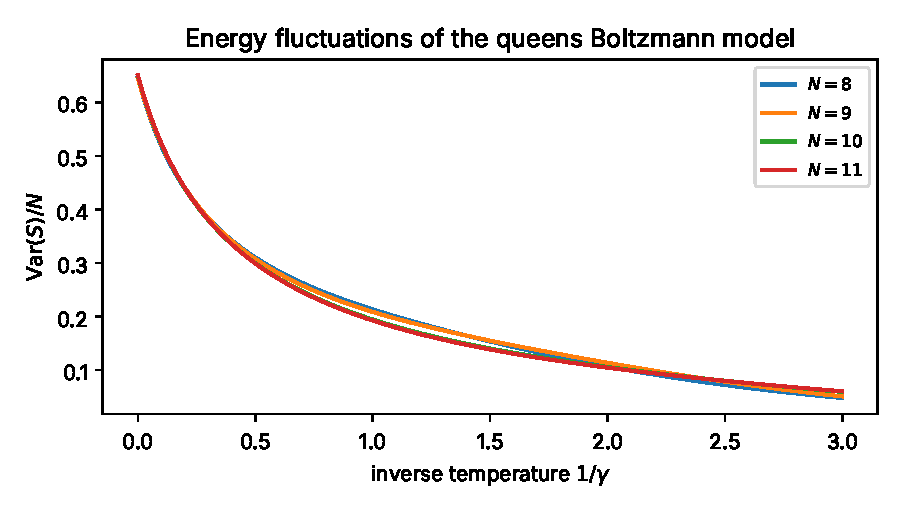
\includegraphics[width=0.85\textwidth]{fig_transition.pdf}
\caption{Energy fluctuations $\Var(S)/N$ of the queens Boltzmann model against inverse temperature, from the exact density of states for $N = 8$ to $11$. The variance is monotone; there is no finite temperature peak.}
\label{fig:transition}
\end{figure}

\section{Problems on the vertical method}

\begin{problem}[The optimal vertical weight]
Characterise the minimax weight $\Omega$ over staircases with $K$ steps and widths in a given range.
\end{problem}

Status. Partially resolved by Chapter~\ref{ch:beyond}: for staircases the stratified\index{stratified sampling} midpoint rule with uniform $\Omega$ is unbiased with mean squared error at most $K \lambda_1^2 / (4n^2)$. We conjecture that no rule can do better than order $K/n^2$ for a staircase with $K$ unknown jump locations, since each jump must be localised to $O(1/n)$ by some node, but we do not prove this lower bound. The constant is open, and the question whether a nonuniform $\Omega$ concentrated near $s = 0$ improves the constant for geometrically decreasing widths, as the queens have, is open.

\begin{problem}[Rates in the quantile coordinate]
Determine the exact dependence of the total error on $K$, $n$ and $\epsilon$ for a staircase whose widths are estimated with relative error $\epsilon$.
\end{problem}

Status. Upper bounds in order of magnitude are given by Chapters~\ref{ch:yakowitz} and~\ref{ch:beyond}, with matching lower bounds not proved: quadrature $O(\sqrt K / n)$, positional $O(\sqrt{\log(1/\rho) / n})$, sampling $O(K \delta)$, the first and third additive and the second relative, in root mean square. The constants are explicit in the stratified case and in the Rao Blackwell\index{Rao Blackwellisation}ised nested case.

\begin{problem}[Two sided promises]
Extend the vertical analysis to $\BPP$.
\end{problem}

Status. Open. The obstacle is that the search to decision reduction of Chapter~\ref{ch:theorems} uses the one sided promise to keep the prefix extension within the promise. For a two sided promise one would need to decide, from a prefix, whether the conditional density is at least $2/3$ or at most $1/3$, and this is a $\BPP$ question again. The known route from $\RP$ to $\BPP$ derandomization is through Andreev, Clementi and Rolim, who show that a hitting set\index{hitting set} generator suffices for $\BPP$ by a nontrivial argument, and the vertical analogue of their argument is not obvious.

\begin{problem}[Hashing versus walking]
Compare the sample complexity of Stockmeyer\index{Stockmeyer's theorem}'s hashing estimator with the vertical walk when both use the same level set sampler\index{level set sampler}.
\end{problem}

Status. Open. With a sampler in place of the $\NP$ oracle, the hashing estimator at hash length $k$ needs to estimate $|S \cap h^{-1}(0)|$, and sampling from $S$ and checking the hash does not do this, since for a pairwise independent $h$ a uniform draw lands in $h^{-1}(0)$ with probability about $2^{-k}$ whatever $|S|$ is, so it estimates the fraction $|S \cap h^{-1}(0)|/|S|$ and carries no information about $|S|$; near the critical length the hit rate is about $1/|S|$ and $O(1/\epsilon^2)$ samples per length do not suffice. We have therefore not completed the comparison, and an earlier estimate of $O(\log|S|/\epsilon^2)$ samples for hashing against $O(K^2/\epsilon^2)$ for the walk should not be relied on. In any case a uniform sampler on $S$ is what hashing needs, and a uniform sampler on $S$ is the bottom rung of the walk, and the walk is the method for producing it. The natural hybrid, which we do not analyse, is to walk to the bottom and hash there, which is what the Jerrum Valiant\index{Valiant, Leslie} Vazirani self reducib\index{self reducibility}ility route does in effect.

\section{Problems on derandomization}

\begin{problem}[Vertical hitting sets]
Find a class of $\RP$ problems beyond $\Pc$ for which the dense level set can be hit by an explicit polynomial size set.
\end{problem}

Status. Open, and by Kabanets and Impagliazzo\index{Kabanets and Impagliazzo} (2004) a deterministic polynomial time algorithm for polynomial identity testing of general arithmetic circuits would imply either that $\mathrm{NEXP} \not\subseteq \Ppoly$ or that the permanent has no polynomial size arithmetic circuits; restricted classes carry no such implication, and explicit hitting sets are known for several (sparse polynomials, by Klivans and Spielman in 2001, and read once oblivious branching programs). One class where this is unconditional is $\mathrm{AC}^0$ by Nisan's generator; the vertical walk for an $\RP$ algorithm whose acceptance predicate is in $\mathrm{AC}^0$ can be derandomized by running it on the $n^{\mathrm{polylog}(n)}$ outputs of Nisan's generator (seed length $\mathrm{polylog}(n)$ for fixed depth), which is quasipolynomial. The polynomial case is open even for $\mathrm{AC}^0$.

\begin{problem}[Deterministic level set hitting for the queens]
Give a deterministic polynomial time procedure that outputs a permutation with at most $m$ attacking pairs for the smallest possible $m$.
\end{problem}

Status. Resolved for the unconditioned problem and open for the conditioned one. Explicit solutions, $m = 0$, are known for all $N \ge 4$: for $N$ coprime to $6$ the permutation $x_i = 2i \bmod N$ is a solution, and Pauls in 1874 and many since have given constructions for all $N$. So the unconditioned level set $\{ S = 0 \}$ is hit deterministically in $O(N)$ time, and the question has content only on conditioned boards, where it is the search version of the $\NP$ complete completion problem.

\section{Problems on the broader program}

\begin{problem}[The Jerrum Valiant Vazirani gap]
Exhibit a non self reducible counting problem for which approximate counting is in $\RP$ but sampling is not known to be.
\end{problem}

Status. Open. Candidates are counting problems defined by non monotone constraints where the self reducibility tree has no uniform structure. The vertical walk counts by sampling level sets, not solutions, and so applies to such problems, but whether it gives an FPRAS\index{FPRAS} without a solution sampler at the bottom is unclear, since the bottom rung is a solution sampler.

\begin{problem}[Lean and the queens]
Formalise the Lorenz\index{Lorenz curve} identity, the product estimator variance bound, and the conditional FPRAS theorem.
\end{problem}

Status. Statements written, proofs open; see Chapter~\ref{ch:lean}, which gives Lean style statements and proof sketches that have not yet been machine checked. The statements are elementary and the main equivalence of Chapter~\ref{ch:theorems} is an assembly of cited theorems; formalising the assembly, with the cited results as axioms, would be a modest project and would produce a machine checked statement of exactly what the program claims.

\section{The shattering depth}
\label{sec:depth}

The third round of computation for this chapter asked a question that the earlier rounds had not: when the bottom level set $\{ S \le 1 \}$ of a board shatters, does the next level set $\{ S \le 2 \}$ shatter too? The answer, on every unconditioned board we have examined, is no, and it changes what the program should ask for.

\begin{problem}[Swap connectivity of the second level set]
Determine the least $m_c(N)$ such that $\{ S \le m_c \}$ is connected under swaps for the unconditioned $N$ queens problem.
\end{problem}

Status. Resolved for $N \le 11$ by exhaustive enumeration of all $N!$ placements with a breadth first search over swaps at every energy threshold. Table~\ref{tab:levelsets} gives the number of swap components of $\{ S \le m \}$ for $m = 0, 1, 2$. The level set $\{ S \le 2 \}$ is connected for every $N$ from $4$ to $11$, so $m_c(N) \le 2$ in this range, and $m_c(N) = 2$ except at $N = 8$, where $\{ S \le 1 \}$ is already connected. At $m = 1$ the level set has many components for $N \ge 9$ ($69$, $253$ and $1121$ for $N = 9$, $10$, $11$), almost all of them small clusters of near solutions containing no solution, as the earlier table showed; at $m = 2$ every one of them is absorbed into a single component. We conjecture that $m_c(N) = 2$ for all $N \ge 9$. The conjecture is needed in the sketch of the conditional FPRAS for $Q(N)$ in Chapter~\ref{ch:program}, where it replaces an argument from monotonicity that the first draft of that proof wrongly relied on: the level sets are nested but the connectivity of a larger one does not follow from the connectivity of a smaller one, and the computation is what supports the claim.

\begin{table}[t]
\centering
\small
\caption{Swap components of the level sets $\{ S \le m \}$ of the unconditioned problem, by exhaustive enumeration. For each $N$: the size of $\{ S \le m \}$ and the number of swap components, for $m = 0$, $1$ and $2$. The level set $\{ S \le 2 \}$ is connected for every $N$ shown.}
\label{tab:levelsets}
\begin{tabular}{rrrrrrr}
\toprule
$N$ & $|\{S \le 0\}|$ & comps & $|\{S \le 1\}|$ & comps & $|\{S \le 2\}|$ & comps \\
\midrule
4 & 2 & 2 & 10 & 2 & 16 & 1 \\
5 & 10 & 10 & 10 & 10 & 66 & 1 \\
6 & 4 & 4 & 64 & 10 & 224 & 1 \\
7 & 40 & 36 & 192 & 22 & 872 & 1 \\
8 & 92 & 84 & 980 & 1 & 3844 & 1 \\
9 & 352 & 304 & 3728 & 69 & 20376 & 1 \\
10 & 724 & 612 & 15128 & 253 & 106056 & 1 \\
11 & 2680 & 2128 & 70336 & 1121 & 584024 & 1 \\
\bottomrule
\end{tabular}
\end{table}

A proof of $m_c(N) \le 2$ would be the natural base of a canonical path\index{canonical paths} argument on $\{ S \le 2 \}$. We do not have one. A proof that $m_c(N) \le c$ for some constant $c$ would already have consequences, since the ratio $N(0) / |\{ S \le c \}|$ should then be at least inverse polynomial, of order $N^{-c}$ by the heuristic that each additional attack can be placed in about $N$ ways; a bound $m_c(N) \le cN$ would not, since by the rate function of Chapter~\ref{ch:entropy} the ratio $N(0) / |\{ S \le cN \}|$ is then exponentially small. The paragraph below explains why the distinction matters.

\begin{problem}[The shattering depth of a board]
For a board $B$ with completions, define the solution depth $m_s(B)$ as the least $m$ such that all completions of $B$ lie in one swap component of the conditioned level set $\{ S \le m \}$, and the shattering depth $m_c(B)$ as the least $m$ such that $\{ S \le m \}$ is itself connected. Determine the distributions of $m_s(B)$ and $m_c(B)$ over random boards and their growth over hard boards.
\end{problem}

Status. The random queens completion model of the previous section showed that random conditioning fragments $\{ S \le 1 \}$. We have now run that model on $300$ instances per $k$ at $N = 12$ and $150$ at $N = 13$, with the fixed queens chosen uniformly subject to pairwise non attack and the instance kept if it has a completion, and the results are in Table~\ref{tab:random2}. About half of the random boards with two to four fixed queens have their completions in more than one component of $\{ S \le 1 \}$: $47\%$ at $N = 12$ with $k = 2$, $62\%$ with $k = 3$, and $54\%$ to $57\%$ at $N = 13$ with $k = 3$ and $4$. The worst boards are severely shattered. A board at $N = 12$ with two fixed queens, at row $0$ column $2$ and row $11$ column $0$, has $42$ completions spread over $30$ components of $\{ S \le 1 \}$, the largest holding $5$ (this board comes from a separate random draw of boards at the same size, not from the $300$ instances of the table, whose most shattered board at $N = 12$ with $k = 2$ has $22$ components); a board at $N = 13$ with three fixed queens has $17$ completions in $15$ components. A greedy adversarial search that moves one fixed queen at a time to increase the number of solution components finds, at $N = 12$ with three fixed queens, a board with $16$ completions in $12$ components and one with $39$ completions in $13$, and with four fixed queens a board whose six completions are all isolated from one another. Shattering of the bottom level set is therefore not rare under random conditioning and can be made severe by a weak adversary, at sizes where the solution derived conditioning of Table~\ref{tab:conditioned} shows nothing of the kind. This is the planted versus random distinction of the satisfiability literature appearing in the queens: a board that was cut out of a solution keeps that solution's component intact, and a board that was not has no such guarantee.

\begin{table}[t]
\centering
\small
\caption{Random boards with $k$ fixed queens and at least one completion, $300$ instances per row at $N = 12$ and $150$ at $N = 13$: mean number of completions, fraction of instances whose completions lie in more than one component of $\{ S \le 1 \}$, mean and maximum number of solution components, and mean and minimum fraction of completions in the largest component.}
\label{tab:random2}
\footnotesize
\begin{tabular}{rrrrrrrr}
\toprule
$N$ & $k$ & mean $N(0)$ & multi & comps & max & giant & min \\
\midrule
12 & 2 & 121.8 & 0.47 & 2.50 & 22 & 0.977 & 0.161 \\
12 & 3 & 15.6 & 0.62 & 2.52 & 11 & 0.826 & 0.111 \\
12 & 4 & 3.2 & 0.46 & 1.63 & 5 & 0.799 & 0.200 \\
12 & 5 & 1.5 & 0.18 & 1.21 & 4 & 0.914 & 0.250 \\
13 & 3 & 59.6 & 0.54 & 2.59 & 15 & 0.944 & 0.118 \\
13 & 4 & 8.7 & 0.57 & 2.22 & 10 & 0.766 & 0.143 \\
13 & 5 & 2.5 & 0.40 & 1.57 & 4 & 0.810 & 0.250 \\
\bottomrule
\end{tabular}
\end{table}

The new fact is what happens one and two levels up. For each of the worst boards we enumerated the conditioned level sets $\{ S \le m \}$ for $m = 2, 3, 4$ and found their swap components. On every one of them all completions lie in a single component of $\{ S \le 2 \}$. The board with $42$ completions in $30$ components of $\{ S \le 1 \}$ has them in one component of $\{ S \le 2 \}$; so does the adversarial board with $39$ completions in $13$ components, and the board with six isolated completions. In every case examined the solution depth is $m_s(B) = 2$: the near solutions with one attack are too sparse to bridge the completions, and the placements with two attacks are dense enough. The level set $\{ S \le 2 \}$ is not itself connected on these boards: it has $94$, $5$ and $13$ components, all but one of them islands of two attack placements that contain no completion. These islands matter, because a chain that samples $\{ S \le 2 \}$ from a completion never reaches them and the fraction of ground states it reports is biased by their mass. One level higher they are absorbed: $\{ S \le 3 \}$ is connected on the first two boards and $\{ S \le 4 \}$ on the third, so the shattering depth is $m_c(B) = 3$ or $4$. On forty random boards with two fixed queens and forty with three, $m_s(B)$ is $1$ on fifteen and $2$ on twenty five of each forty, never more, and $m_c(B)$ is $3$ on seventy five of the eighty, $2$ on three, and $4$ on two. Table~\ref{tab:depth} gives the counts for the three boards, and with them the price of climbing: the ratio $N(0) / |\{ S \le m_c \}|$ is between $0.0005$ and $0.002$ on these boards and about $0.001$ on average over the random ones, against a ratio $N(0) / |\{ S \le 1 \}|$ near $0.04$ on unconditioned boards ($0.039$ at $N = 12$). The price of two levels is a factor of thirty to forty in the bottom ratio, and so of thirty to forty in the number of samples a Bernoulli estimate of that ratio needs.

\begin{table}[t]
\centering
\small
\caption{Depths of three severely shattered boards at $N = 12$. The fixed queens are given as (row, column) pairs; $N(0)$ is the number of completions; for each $m$ the size of the conditioned level set $\{ S \le m \}$, its number of swap components, and the number of those containing a completion. The shattering depth is the first $m$ with one component: $3$, $3$ and $4$. The ratios $N(0) / |\{ S \le m_c \}|$ are $0.0005$, $0.0020$ and $0.0011$.}
\label{tab:depth}
\footnotesize
\begin{tabular}{p{3.2cm}rrrrr}
\toprule
board & $N(0)$ & $m$ & size & comps & with sol \\
\midrule
$(0,2)$, $(11,0)$ & 42 & 1 & 1285 & 447 & 30 \\
 & & 2 & 15549 & 94 & 1 \\
 & & 3 & 87763 & 1 & 1 \\
\midrule
$(7,11)$, $(10,5)$, $(11,10)$ & 39 & 1 & 515 & 98 & 13 \\
 & & 2 & 4335 & 5 & 1 \\
 & & 3 & 19126 & 1 & 1 \\
\midrule
$(0,7)$, $(1,11)$, $(8,10)$, $(11,8)$ & 6 & 1 & 49 & 23 & 6 \\
 & & 2 & 448 & 13 & 1 \\
 & & 3 & 1928 & 2 & 1 \\
 & & 4 & 5265 & 1 & 1 \\
\bottomrule
\end{tabular}
\end{table}

This changes the shape of the mixing conjecture. The vertical walk does not need the bottom rung; it needs some rung whose level set is connected and well mixed and whose ratio to the ground state is not too small. The following statement makes that precise.

\begin{theorem}[Rung skipping]
\label{thm:rungskip}
Let $B$ be a board with completions and let $m \ge m_c(B)$. Suppose the swap chain on the conditioned level set $\{ S \le j \}$ is irreducible and mixes in time $T$, polynomial in $N$, for every $j \ge m$, that $|\{ S \le j \}| / |\{ S \le j + 1 \}| \ge 1 / q(N)$ for every $j \ge m$ and a polynomial $q$, and that $N(0) / |\{ S \le m \}| \ge 1 / p(N)$ for a polynomial $p$. Let $K$ be the number of rungs above $m$, that is, the number of $j \ge m$ with $\{ S \le j \}$ not the whole board. Then the vertical walk that estimates $N(0) / |\{ S \le m \}|$ directly, as the fraction of ground states among samples from $\{ S \le m \}$, and the ratios $|\{ S \le j \}| / |\{ S \le j + 1 \}|$ for $j \ge m$ by the product estimator, is an FPRAS for the completion count with cost $O((K^3 q(N) + p(N)) \epsilon^{-2} T \log (K/\delta))$ for confidence $1 - \delta$.
\end{theorem}

\begin{proof}
The bottom ratio is a Bernoulli mean with success probability at least $1/p(N)$, so $O(p(N) \epsilon^{-2} \log (1/\delta))$ samples give relative error $\epsilon / 2$ with the stated confidence. Each rung ratio $|\{ S \le j \}| / |\{ S \le j + 1 \}|$ above $m$ is a Bernoulli mean, under the uniform law on $\{ S \le j + 1 \}$, of at least $1/q(N)$, by the rung ratio hypothesis, so $O(q(N) K^2 \epsilon^{-2} \log (K/\delta))$ samples from a chain with mixing time $T$ estimate it to relative error $\epsilon / (2K)$, and the product of the $K$ estimates has relative error about $\epsilon / 2$, so that with the bottom ratio the total is within a constant multiple of $\epsilon$, which rescaling $\epsilon$ removes; this is the argument of the conditional FPRAS theorem of Chapter~\ref{ch:program}, run on the conditioned level sets instead of the unconditioned ones. The condition $m \ge m_c(B)$ is necessary rather than sufficient for the mixing hypothesis: below the shattering depth the level set is disconnected and no chain on it is irreducible, and above it irreducibility at every level $j \ge m$ is part of what is assumed, since the connectivity of $\{ S \le m \}$ does not by itself imply that of $\{ S \le m + 1 \}$. Solution depth is not enough: a chain on $\{ S \le m_s \}$ started from a completion samples the completion component uniformly but never the islands, and the ground state fraction it reports is too large by the factor of the island mass.
\end{proof}

The theorem relocates the question. On the boards examined at $N = 12$, $m = 3$ suffices on all but two of eighty, $m = 4$ on those two, and larger $N$ need $m = 4$ more often (Table~\ref{tab:depthgrowth}), and the price is a factor of thirty to forty in the bottom ratio, which is nothing. The mixing conjecture for hard boards is then not that $\{ S \le 1 \}$ shatters, which it demonstrably does on easy random boards as well, but that the shattering depth grows: that on reduction boards from hard formulas $m_c(B)$ is of order $N$ or larger, so that the first connected level set has exponentially more placements than completions and the Bernoulli estimate of the bottom ratio takes exponential time. Equivalently, the hardness lives not in the disconnection of one level set but in the depth to which the disconnection persists. We state this as the revised conjecture.

\begin{conjecture}[Shattering depth on hard boards]
\label{conj:shatterdepth}
There is a family of boards $B_N$ from the Gent Jefferson Nightingale reduction applied to hard formulas with $m_c(B_N) \ge c N$ for a constant $c > 0$, and for such boards the ratio $N(0) / |\{ S \le m_c(B_N) \}|$ is exponentially small in $N$.
\end{conjecture}

The conjecture is testable: the enumeration that found $m_c = 3$ on the random boards runs in seconds at $N = 12$, and on a reduction board of moderate size it would find the depth directly. Its negation at every size, $m_c(B) \le c$ for a constant $c$ on all boards, together with polynomial mixing above the depth, an inverse polynomial bound on $N(0) / |\{ S \le c \}|$ and on the rung ratios, would give $\NP = \RP$ by the rung skipping theorem and the main equivalence, and this is now the sharpest form of the program's Monte Carlo half that we can state: find the shattering depth of hard boards.

\begin{problem}[Queenon tilted proposals]
Does a swap proposal tilted towards the queenon density mix faster than the uniform swap on the bottom level set?
\end{problem}

Status. Resolved negatively at the sizes tested. Simkin\index{Simkin's theorem}'s queenon\index{queenon} is the limiting density of queen positions in a uniform solution, and one might hope that proposing swaps that move queens towards the dense parts of the board would raise the acceptance rate of the bottom rung chain. We estimated the density from the $73712$ solutions at $N = 13$, interpolated it to an $N \times N$ board, and ran the swap chain on $\{ S \le 1 \}$ with the pair $(i, j)$ proposed with probability proportional to $q(i, x_j) \, q(j, x_i)$, the product of the densities at the two squares the swap would occupy, with the Metropolis Hastings correction that keeps the uniform target. Figure~\ref{fig:queenon} shows the density and the comparison. The density is far from flat: along the middle row it is $1.42$ times uniform at the edges and $0.79$ at the centre, and along the top row $0.49$ at the corners and $1.42$ at the centre, the pattern that Simkin's queenon predicts. The tilt does not help. At $N = 12, 16, 20, 24$ the integrated autocorrelation times of the first row column are $246, 402, 775, 716$ proposals for the uniform swap and $312, 489, 956, 761$ for the tilted swap, with standard deviations over five runs of sixteen to forty eight percent, and the acceptance rates fall from $0.061, 0.046, 0.036, 0.032$ to $0.052, 0.040, 0.033, 0.029$. The tilted chain is slightly slower at every size. The reason is that the queenon is a one point marginal and the constraints are pairwise: the squares that are dense are dense because many solutions use them, not because a given near solution can be repaired by moving a queen there, and proposing moves towards them lowers the acceptance rate without shortening the repair paths. A proposal that could help would have to use the conditional density of a square given the other queens, which is the thing the chain is trying to sample. The problem that remains open is whether a two point tilt, using Simkin's bound on the density of attacking pairs, does any better; we expect not.

\begin{figure}[t]
\centering
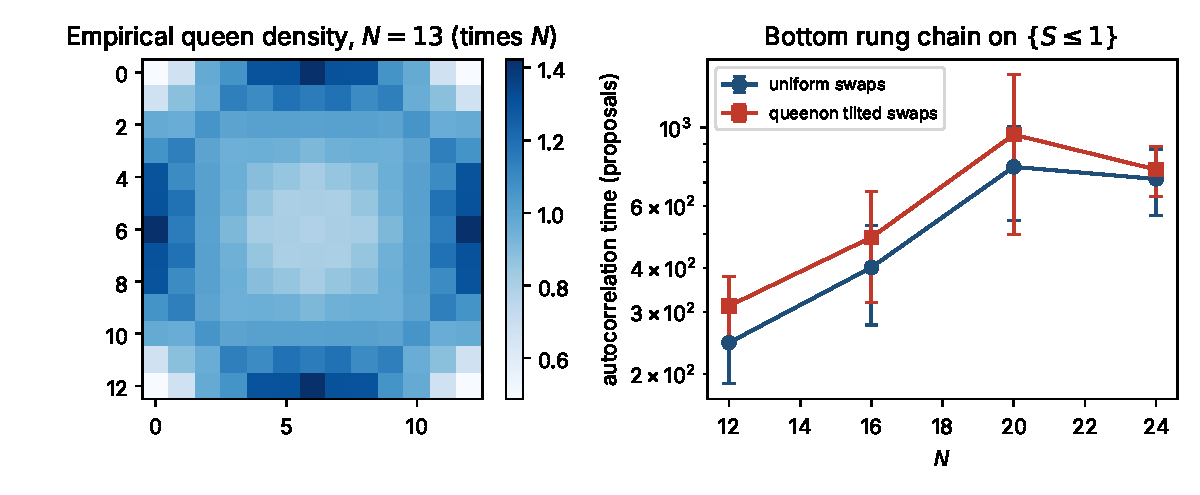
\includegraphics[width=\textwidth]{fig_queenon.pdf}
\caption{Left: the empirical queen density at $N = 13$, from all $73712$ solutions, scaled so that uniform is one. Right: autocorrelation time of the bottom rung chain with uniform and queenon tilted swap proposals, mean and standard deviation over five runs.}
\label{fig:queenon}
\end{figure}


\section{The fourth round: gaps, depths and windows}
\label{sec:round4}

This round carries out three computations that the earlier rounds left open: the spectral gap of the bottom rung chain, the growth of the shattering depth with $N$, and the divergence of the solution law from Markov window families. One of them moved the program's conjecture; one of them showed that a depth of three does not suffice on all boards; and one closed a door that Chapter~\ref{ch:ce} had left ajar.

\begin{problem}[The spectral gap of the bottom rung chain]
Compute the spectral gap of the swap chain on the giant component $G_N$ of $\{ S \le 1 \}$ and its growth with $N$.
\end{problem}

Status. Computed exactly for $N = 8$ to $12$ by a sparse eigensolver on the transition matrix of the chain, which has $980$, $3636$, $14824$, $69096$ and $355860$ states; the last took over an hour, the top of the spectrum being nearly degenerate. Table~\ref{tab:gap} gives the relaxation time $1 / \gamma$ of the chain in proposed swaps, the relaxation time restricted to the subspace of functions invariant under the eight symmetries of the board, which is the one that governs every symmetric observable and in particular the ground state indicator that the walk averages, the conductance of the cut defined by the sign of the second eigenvector, and the symmetry under which the second eigenvector is antisymmetric.

\begin{table}[t]
\centering
\small
\caption{The swap chain on the giant component $G_N$ of $\{ S \le 1 \}$: number of states, relaxation time $1/\gamma$ in proposed swaps, relaxation time on the symmetric subspace, the conductance of the sign cut of the second eigenvector, and the symmetry under which that eigenvector is antisymmetric. The three smallest nonzero eigenvalues of $I - P$ for the lazy chain are $0.00166, 0.00182, 0.00261$ at $N = 8$; $0.001127, 0.001127, 0.001138$ at $N = 9$; $0.000910, 0.000914, 0.000914$ at $N = 10$; $0.000571, 0.000571, 0.000572$ at $N = 11$; and $0.000484, 0.000484$ for the first two at $N = 12$, where the symmetry analysis was not run.}
\label{tab:gap}
\begin{tabular}{rrrrrl}
\toprule
$N$ & states & $1/\gamma$ & symmetric & $\Phi$(cut) & antisymmetric under \\
\midrule
8 & 980 & 301 & 275 & 0.0070 & both reflections \\
9 & 3636 & 444 & 433 & 0.0077 & transpose \\
10 & 14824 & 549 & 547 & 0.0072 & transpose \\
11 & 69096 & 875 & 874 & 0.0073 & half turn \\
12 & 355860 & 1033 & & 0.0060 & \\
\bottomrule
\end{tabular}
\end{table}

Three things are in the table. First, the relaxation time grows faster than the autocorrelation time of Chapter~\ref{ch:experiments2}: the pairwise exponents are $3.3$, $2.0$, $4.9$ and $1.9$ and the least squares exponent over $N = 8$ to $12$ is $3.1$, against the $1.76$ of the first row column to $N = 32$. The two are not in conflict, since the autocorrelation time of one observable is a lower bound for the relaxation time up to a factor of about two and the first row column is far from the slowest function, but the exponent that the expansion conjecture of Chapter~\ref{ch:mixingproof} has to deliver is the larger one. Second, the top of the spectrum is nearly degenerate: at $N = 10$ and $11$ the three smallest nonzero eigenvalues agree to two or three figures, and the second eigenvector is antisymmetric under a board symmetry, the transpose at $N = 9$ and $10$ and the half turn at $N = 11$, while the symmetric subspace relaxes at almost the same rate. The symmetry explains the particular eigenvector and not the slowness. A band of near degenerate slow modes is the spectral signature of many bottlenecks of comparable strength, and the landscape of Chapter~\ref{ch:mixingproof} says what they are: clusters of near solutions attached to the giant component by few swaps. Third, the sign cut of the second eigenvector has conductance between $0.006$ and $0.008$ at every $N$, so it is not the bottleneck; by Cheeger's inequality the true conductance satisfies $\gamma / 2 \le \Phi \le \sqrt{2 \gamma}$, that is, $0.0005 \le \Phi_{12} \le 0.044$, and the bottleneck sets are not symmetry halves but something smaller that the eigenvector does not reveal directly. Finding them is the next step on this problem: the second eigenvector restricted to the symmetric subspace, thresholded at levels other than zero, and the clusters it isolates.

The practical reading is that the expansion conjecture should be stated with $c'$ near $3$ rather than near $2$, that the bottom rung needs of order $N^3$ swaps per effective sample for the worst observable and of order $N^{1.8}$ for the first row column over the range measured, and that the computation at $N = 13$ with a symmetry reduced matrix, which has eight times fewer states, is within reach and would tell whether the pairwise exponents, which swing between $1.9$ and $4.9$, are settling.

\begin{problem}[Growth of the shattering depth]
Determine how $m_c(B)$ grows with $N$ on random boards.
\end{problem}

Status. Measured at $N = 14$ and partly at $N = 16$, with a C implementation of the enumeration that handles level sets of twenty million placements. Table~\ref{tab:depthgrowth} gives the distribution of the solution depth $m_s$ and the shattering depth $m_c$ over the random boards at each $(N, k)$, and the mean ratio $N(0) / |\{ S \le m_c \}|$ at the depth. The fraction of boards that need $m_c = 4$ grows. At $N = 12$ the level set was connected at $m = 3$ on $75$ of $80$ boards (already at $m = 2$ on three more); at $N = 14$ it is connected at $m = 3$ on $22$ of $40$ and needs $m = 4$ on the other $18$, and at $N = 16$ with four fixed queens it is connected at $m = 3$ on one board of eight and needs $m = 4$ on the other seven, while with five fixed queens it is connected at $m = 3$ on three of eight and needs $m = 4$ on the other five. The solution depth does not grow: completions reconnect at $m = 1$ or $2$ at every size. The price grows with the depth, from $1 \times 10^{-3}$ at $N = 12$ to $3 \times 10^{-4}$ at $N = 14$ and $1 \times 10^{-4}$ to $2 \times 10^{-4}$ at $N = 16$, a factor of about three for every two rows. Since $k$ changes with $N$ in the table ($2$ and $3$ at $N = 12$ and $14$, $4$ and $5$ at $N = 16$), the effects of $N$ and of $k$ are confounded.

\begin{table}[t]
\centering
\small
\caption{Growth of the depths with $N$ on random boards with $k$ fixed queens, forty boards per row at $N = 12$, twenty at $N = 14$ and eight at $N = 16$: the number of boards with solution depth $m_s = 1$ and $2$, with shattering depth $m_c = 2$, $3$ and $4$, and the mean of $N(0) / |\{ S \le m_c \}|$ over the boards.}
\label{tab:depthgrowth}
\begin{tabular}{rrrrrrrr}
\toprule
$N$ & $k$ & $m_s{=}1$ & $m_s{=}2$ & $m_c{=}2$ & $m_c{=}3$ & $m_c{=}4$ & mean ratio \\
\midrule
12 & 2 & 15 & 25 & 0 & 39 & 1 & $7.9 \times 10^{-4}$ \\
12 & 3 & 15 & 25 & 3 & 36 & 1 & $1.3 \times 10^{-3}$ \\
14 & 2 & 15 & 5 & 0 & 12 & 8 & $3.0 \times 10^{-4}$ \\
14 & 3 & 13 & 7 & 0 & 10 & 10 & $2.8 \times 10^{-4}$ \\
16 & 4 & 5 & 3 & 0 & 1 & 7 & $1.0 \times 10^{-4}$ \\
16 & 5 & 4 & 4 & 0 & 3 & 5 & $1.7 \times 10^{-4}$ \\
\bottomrule
\end{tabular}
\end{table}

This shows that a depth of three does not suffice on every board measured, and it changes the conjecture. The hypothesis that the depth is bounded on random boards and grows only on reduction boards is no longer clearly the best reading of the data; the typical depth on random boards moves by about one between $N = 12$ and $16$, and the question is whether it keeps moving and at what rate. If $m_c$ grows like $\log N$ the price $N(0) / |\{ S \le m_c \}|$ is only quasi-polynomial, of order $N^{c \log N}$, by the heuristic that each extra attack costs a factor of order $N$, and the rung skipping theorem gives a quasi-polynomial and not a polynomial walk on random boards; only a bounded $m_c$ gives an inverse polynomial price. If $m_c$ grows like $cN$ the price is exponential and the walk fails on random boards, which would place the random queens completion problem with the problems on which Monte Carlo fails on average, and would make the reduction board question moot for this chain. The data to $N = 16$ cannot tell $\log_2 N$ from $N / 4$: rounded down, both give $3$ at $N = 12$ and $4$ at $N = 16$. The measurement that decides is the depth at $N = 20$ and $24$, which the C enumeration can reach for level sets up to about $10^8$ placements, and at those sizes $\log_2 N$ rounded down predicts $4$ and $N / 4$ predicts $5$ to $6$. We state the revised conjecture with the alternative it must beat.

\begin{conjecture}[Depth growth]
\label{conj:depthgrowth}
On random boards with a fixed number of fixed queens, $m_c(B) = O(1)$ with high probability, so that the price of rung skipping is inverse polynomial. The data to $N = 16$ do not exclude slow growth: $m_c(B) = O(\log N)$ would make the price quasi-polynomial, and the alternative, $m_c(B) \ge cN$, would make the vertical walk exponential on random boards.
\end{conjecture}

The unconditioned problem is unaffected: $\{ S \le 2 \}$ is connected for $N \le 11$ with no fixed queens, and the realistic prize of Chapter~\ref{ch:program} rests on the connectivity of $\{ S \le 2 \}$ or on the giant component of $\{ S \le 1 \}$, together with the rung ratio hypothesis of its theorem, and not on the depth of a conditioned board.

\begin{problem}[Markov window families]
Compute the divergence from the uniform law on solutions to its projection on the order $k$ Markov sequential family, as a function of $k$ and $N$.
\end{problem}

Status. Computed exactly for $N = 8$ to $13$ from all solutions. For the family $g(x) = \prod_i g_i(x_i \mid x_{i-k}, \dots, x_{i-1})$ with unrestricted window conditionals, the minimum divergence is
\[
D_k(N) = \sum_{i=1}^N H(X_i \mid X_{i-k}, \dots, X_{i-1}) - \log Q(N) ,
\]
with the window truncated at row $1$ for $i \le k$, by the same entropy decomposition as Theorem~\ref{thm:product} of Chapter~\ref{ch:ce}, the conditional entropies being those of a uniform random solution, and Table~\ref{tab:window} gives it. Two facts are in the table. For fixed window $k$ the divergence grows linearly in $N$: $D_2$ increases by about $2.4$ nats per row and $D_3$ by about $2.9$ from $N = 10$ on, so the information that the diagonal constraints carry beyond any fixed window is more than two nats per queen, and, if the linear growth seen for $N = 8$ to $13$ continues, the relative variance of importance sampling from any such family, at least $e^{D_k} - 1$, is exponential in $N$. And the window needed to bring the divergence below one nat is about half the board: $k = 3, 4, 5, 5, 6, 7$ for $N = 8$ to $13$. This is the cross entropy form of the shattering depth that Chapter~\ref{ch:ce} asked for, and it is linear in $N$. A sequential family whose conditionals see only a window of fixed width, which is what the cross entropy method uses for permutation problems, cannot give a polynomial time counter for the queens; a family whose conditionals see the whole history can, in principle, since $D_{N-1} = 0$, but the representation question of Chapter~\ref{ch:gbc} is then whether a conditional of the full history can be computed by a polynomial size circuit to within $O(\log N)$ nats, and the window computation says the circuit cannot be local.

\begin{table}[t]
\centering
\small
\caption{Divergence $D_k(N)$ in nats from the uniform law on solutions to the best order $k$ Markov sequential family, exact from all solutions, and the least $k$ with $D_k < 1$.}
\label{tab:window}
\begin{tabular}{rrrrrrrrr}
\toprule
$N$ & $Q(N)$ & $D_0$ & $D_1$ & $D_2$ & $D_3$ & $D_4$ & $D_5$ & $k(D_k < 1)$ \\
\midrule
8 & 92 & 11.4 & 7.3 & 3.0 & 0.82 & 0.21 & 0 & 3 \\
9 & 352 & 13.7 & 10.2 & 5.9 & 2.1 & 0.67 & 0.26 & 4 \\
10 & 724 & 16.2 & 12.6 & 8.1 & 3.6 & 1.15 & 0.37 & 5 \\
11 & 2680 & 18.2 & 14.9 & 11.0 & 6.3 & 2.45 & 0.81 & 5 \\
12 & 14200 & 20.0 & 16.8 & 13.3 & 9.7 & 5.13 & 2.03 & 6 \\
13 & 73712 & 21.9 & 18.7 & 15.4 & 12.3 & 8.28 & 4.31 & 7 \\
\bottomrule
\end{tabular}
\end{table}

The three computations point the same way. The chain's relaxation time grows like $N^3$, the fraction of conditioned boards that need the deeper level set grows with $N$, and the window a sequential family needs grows like $N / 2$: on every axis the queens get harder with $N$ faster than the first measurements suggested. Nothing in this round is a proof.

\section{What has moved}

Since the first draft, ten problems have changed status. The repair neighbourhood is quadratic on average and empty for a vanishing set of stragglers. The random completion model shows a satisfiability threshold near $k/N = 0.35$ to $0.4$ at $N = 12$ and, on three hundred instances, a bottom level set that has more than one solution component on about half of the random boards with two to four fixed queens and fragments severely on the worst of them. The physics transition is absent for $N \le 11$. The connectivity problem is resolved for $N \le 13$ with the giant component result on unconditioned boards, which persists under solution derived conditioning to $N = 17$ and does not persist on about half of the boards under random conditioning at $N = 12$. The second level set $\{ S \le 2 \}$ is connected for $N \le 11$ on unconditioned boards; on shattered boards the completions reconnect in $\{ S \le 2 \}$ and the level set itself reconnects at a depth that is two to four at $N = 12$, three or four at $N = 14$, and three or four at $N = 16$ on the boards examined; the data do not yet show that the shattering depth grows with $N$, and if it does the question is whether like $\log N$ or like $N$. The spectral gap of the bottom rung chain is known exactly to $N = 12$: its relaxation time grows like $N^3$, with a nearly degenerate band of slow modes that the board symmetries do not explain. The Markov window a sequential family needs to come within a nat of the solution law is half the board. The queenon tilted proposal does not accelerate the bottom rung. The finite size correction problem has a numerical conjecture, $\beta = 0$ and $C \approx 2.4$, which the fit supports only to $|\beta| \lesssim 0.1$ given Simkin's error bar. The deterministic hitting problem is resolved trivially for unconditioned boards by the explicit constructions. The problems that remain, and that matter most, are two: the rate of growth of the shattering depth on random boards, which decides whether the walk is polynomial on average, and the depth on reduction boards, which decides whether it is polynomial in the worst case. The enumeration that measures both runs in minutes at $N = 16$, and the next sizes are $20$ and $24$.


\chapter*{Epilogue}
\addcontentsline{toc}{chapter}{Epilogue}
\markboth{Epilogue}{}

A reader who has come this far deserves a plain statement of what has been established, what has been conjectured, and what we think should happen next.

Established: that every randomized algorithm and every counting problem has a Lorenz curve, that the Lorenz curve of a randomized decision is a single step whose location decides the question, that the Lorenz curve of a structured counting problem has polynomially many steps whose widths are the density of states, that the walk down the curve is polynomial in its number of rungs and in its quadrature error, and that the only part of the walk whose cost is not controlled analytically is the production of a draw from a level set. Established also, by proof, that the walk is an FPRAS whenever the level set chains mix, with explicit constants; that it may skip any rung whose level set is disconnected, at a price equal to the ratio of the ground state to the first connected level; that the mixing of the bottom chain on unconditioned boards is reducible to an expansion property of a family of finite graphs; and that no importance sampling proposal of product form, which is what the cross entropy method uses, can beat crude Monte Carlo on the queens by more than the factor $e^{d}$ of Theorem~\ref{thm:product}, which is at most $2$ for $8 \le N \le 12$.

Computed: that the solutions of the unconditioned problem lie, with a vanishing number of exceptions, in one swap component of the level set with at most one attack, for $N \le 13$; that this component is held together not by direct repairs but by paths through near solutions, some of which lie eight swaps from the nearest solution; that the bottom chain on it has autocorrelation time growing like $N^{1.8}$ to $N = 32$; that the level set with at most two attacks is connected for $N \le 11$; that random conditioning by two to four queens gives more than one solution component on about half of the boards at $N = 12$ (the giant component holds down to 11 to 20 percent of the solutions on the worst) while conditioning by queens of a solution keeps at least 96 percent in the giant component; and that on every shattered board examined the completions reconnect two attacks up and the level set itself three or four attacks up, with one exception at $N = 12$ where two suffice, so that the shattering depth, the quantity on which the program now turns, is between two and four wherever it has been measured; that the spectral gap of the bottom chain is known exactly for $N = 8$ to $12$, with relaxation time growing roughly like $N^3$ (against the autocorrelation time $N^{1.8}$ of the sampled chain); and that the divergence of the solution law from the best Markov sequential family has been computed (Chapter~\ref{ch:open}).

Conjectured: that the swap graph on the giant component has inverse polynomial conductance, which is the vertical form of a polynomial algorithm for $Q(N)$ and is the realistic prize; that on boards encoding hard formulas the shattering depth grows linearly with $N$, so that the first connected level set has exponentially more placements than completions and the walk fails on them, which is the vertical form of $\NP \neq \RP$; that the single level set of an $\RP$ algorithm, which has density at least a half, can nonetheless be hit by a deterministic polynomial size set, which is the vertical form of $\Pc = \RP$; and that the three conjectures are compatible because a dense level set and a sparse one are different objects, the first hit by a fixed set of points and the second reachable only by a chain.

Next: the shattering depth of a reduction board, which the enumeration of Chapter~\ref{ch:open} can measure in seconds at $N = 12$ and which no one has measured; and the search for a class of $\RP$ problems whose level sets can be hit explicitly. We have given the problems their numbers. We hope to see them solved, by ourselves or by others, and we expect that the solutions, when they come, will be stated on the unit interval.

\appendix

\chapter{Algorithms}
\label{app:alg}

\section{Nested sampling}

Input: a prior sampler for $P$, a likelihood $L$, a number $n$ of live points, a tolerance $\epsilon$.

\begin{enumerate}
\item Draw $x_1, \dots, x_n$ from $P$. Set $Z = 0$, $X = 1$, $k = 0$.
\item Repeat:
\begin{enumerate}
\item Let $y = \min_i L(x_i)$ and let $i^*$ attain it. Set $k = k + 1$, $X_{\mathrm{new}} = e^{-k/n}$, $Z = Z + y \, (X - X_{\mathrm{new}})$, $X = X_{\mathrm{new}}$.
\item Replace $x_{i^*}$ by a draw from $P$ restricted to $\{ L > y \}$.
\item If $X \max_i L(x_i) < \epsilon Z$, add $(X / n) \sum_i L(x_i)$ to $Z$ and stop.
\end{enumerate}
\end{enumerate}

The conditioned draw in step (b) is the only step whose cost depends on the problem. For the queens it is a Markov chain on permutations with fewer than $-\log y$ attacking pairs.

\section{Split sampling with a discrete ladder}

Input: a sampler, an energy $S$, a quantile fraction $\rho \in (0, 1)$, a sample size $M$ per level.

\begin{enumerate}
\item Set $t = 0$, $m_0 = \infty$, $\hat Z = 1$.
\item Repeat:
\begin{enumerate}
\item Draw $x^{(1)}, \dots, x^{(M)}$ from $P$ restricted to $\{ S \le m_t \}$.
\item Set $m_{t+1}$ to the $\rho$ quantile of $\{ S(x^{(i)}) \}$, so that a fraction at least $\rho$ of the sample has $S \le m_{t+1}$. If $m_{t+1} = m_t$, set $m_{t+1} = m_t - 1$.
\item If $m_{t+1} = 0$, set $\hat Z = \hat Z \cdot \#\{ i : S(x^{(i)}) = 0 \} / M$ and stop.
\item Otherwise set $\hat Z = \hat Z \cdot \#\{ i : S(x^{(i)}) \le m_{t+1} \} / M$, $t = t + 1$.
\end{enumerate}
\item Output $\hat Z \cdot |\cX|$ as the estimate of $N(0)$.
\end{enumerate}

With the flat histogram refinement of Chapter~\ref{ch:vertical} the fraction $\rho$ is replaced by a weight $\omega(m)$ on all levels that is updated until each level is visited equally often.

\section{Wang Landau}

Input: an energy $S$ with levels $0, \dots, K$, a flatness tolerance $c$ (we use $c = 0.2$), an initial modification factor $f_0 = e$.

\begin{enumerate}
\item Set $\log g(s) = 0$ and $H(s) = 0$ for all $s$. Set $f = f_0$.
\item Repeat until $f < 1 + 10^{-8}$:
\begin{enumerate}
\item Propose a move $x \to x'$ and accept it with probability
\[ \min\{1, \, g(S(x)) / g(S(x'))\}. \]
\item Set $\log g(S(x)) \leftarrow \log g(S(x)) + \log f$ and $H(S(x)) \leftarrow H(S(x)) + 1$ for the current state.
\item When $\min_s H(s) > (1 - c) \cdot \mathrm{mean}_s H(s)$, set $H \equiv 0$ and $f \leftarrow \sqrt f$.
\end{enumerate}
\item Output $g(s) / \sum_s g(s) \cdot |\cX|$ as the estimate of $N(s)$.
\end{enumerate}

The flat histogram condition in step (c) is the condition that the weight $1/g$ has equalised the visitation of the energy levels, which in the vertical coordinate is the condition that the sampler spends equal time on each stair.

\chapter{Exact Counts}
\label{app:counts}

Table~\ref{tab:counts} records the known values of $Q(N)$ for $4 \le N \le 27$ together with the ratio to $N!$. The values are those tabulated in the On-Line Encyclopedia of Integer Sequences, entry A000170, and come from exhaustive computation by others: $Q(25)$ by Kise and coauthors (2005), $Q(26)$ by the Queens@TUD project of Preusser, Engelhardt and coauthors (2009), and $Q(27)$ by Preusser and Engelhardt~\cite{PreusserEngelhardt}. The book's own scripts enumerate permutations exhaustively only for small $N$ (density of states for $N \le 11$, low energy level sets up to $N = 13$ on unconditioned boards and to $N = 17$ on conditioned boards).

\begin{table}[h]
\centering
\small
\caption{Number of solutions $Q(N)$ of the $N$ queens problem.}
\label{tab:counts}
\begin{tabular}{rrl}
\toprule
$N$ & $Q(N)$ & $\log_{10}(Q(N) / N!)$ \\
\midrule
4 & 2 & $-1.08$ \\
5 & 10 & $-1.08$ \\
6 & 4 & $-2.26$ \\
7 & 40 & $-2.10$ \\
8 & 92 & $-2.64$ \\
9 & 352 & $-3.01$ \\
10 & 724 & $-3.70$ \\
11 & 2680 & $-4.17$ \\
12 & 14200 & $-4.53$ \\
13 & 73712 & $-4.93$ \\
14 & 365596 & $-5.38$ \\
15 & 2279184 & $-5.76$ \\
16 & 14772512 & $-6.15$ \\
17 & 95815104 & $-6.57$ \\
18 & 666090624 & $-6.98$ \\
19 & 4968057848 & $-7.39$ \\
20 & 39029188884 & $-7.79$ \\
21 & 314666222712 & $-8.21$ \\
22 & 2691008701644 & $-8.62$ \\
23 & 24233937684440 & $-9.03$ \\
24 & 227514171973736 & $-9.44$ \\
25 & 2207893435808352 & $-9.85$ \\
26 & 22317699616364044 & $-10.26$ \\
27 & 234907967154122528 & $-10.67$ \\
\bottomrule
\end{tabular}
\end{table}

The last column decreases by approximately $0.41 = 0.942 / \ln 10$ per unit of $N$ once $N$ exceeds about 15, in agreement with Simkin's constant.

\chapter{Glossary of Complexity Classes}
\label{app:glossary}

The classes used in the book, with one line definitions and the inclusions among them. Throughout, polynomial means polynomial in the input length $n$.

\begin{description}[style=nextline]
\item[$\Pc$] Languages decided by a deterministic algorithm in polynomial time.
\item[$\NP$] Languages with polynomial time verifiable certificates. $\Pc \subseteq \NP$.
\item[$\mathrm{co}\NP$] Complements of $\NP$ languages.
\item[$\ZPP$] Languages decided by a randomized algorithm that is always correct and runs in expected polynomial time. $\ZPP = \RP \cap \coRP$.
\item[$\RP$] Languages decided by a randomized polynomial time algorithm that never accepts a string outside the language and accepts each string inside with probability at least $\tfrac12$. $\Pc \subseteq \ZPP \subseteq \RP \subseteq \NP$.
\item[$\coRP$] Complements of $\RP$ languages. Primality was in $\coRP$ before 2002; polynomial identity testing is in $\coRP$.
\item[$\BPP$] Languages decided by a randomized polynomial time algorithm with two sided error at most $\tfrac13$. $\RP \subseteq \BPP$; $\BPP \subseteq \Sigma_2^p \cap \Pi_2^p$ (Sipser, G\'acs, Lautemann); $\BPP \subseteq \Ppoly$ (Adleman for $\RP$, Bennett and Gill for $\BPP$).
\item[$\mathrm{PP}$] Languages decided by a randomized polynomial time algorithm with acceptance probability greater than $\tfrac12$ on strings inside and at most $\tfrac12$ outside, with no gap. $\NP \subseteq \mathrm{PP}$ and $\Pc^{\mathrm{PP}} = \Pc^{\sharpP}$.
\item[$\sharpP$] Functions counting the certificates of an $\NP$ relation. The permanent, $\#\mathrm{SAT}$ and the queens completion count are $\sharpP$ complete.
\item[$\oplus\Pc$] Languages of the form $\{ x : f(x) \text{ odd} \}$ for $f \in \sharpP$. $\NP \subseteq \RP^{\oplus\Pc}$ (Valiant and Vazirani).
\item[$\PH$] The polynomial hierarchy, the union of $\Sigma_k^p$ over $k$, where $\Sigma_k^p$ is defined by $k$ alternating quantifiers with a polynomial time predicate. $\PH \subseteq \Pc^{\sharpP}$ (Toda).
\item[$\Ppoly$] Languages decided by polynomial size circuit families, not necessarily uniformly computable.
\item[$\mathrm{E}$, $\mathrm{EXP}$, $\mathrm{NEXP}$] Deterministic time $2^{O(n)}$, deterministic time $2^{\mathrm{poly}(n)}$, and nondeterministic time $2^{\mathrm{poly}(n)}$.
\item[FPRAS] A fully polynomial randomized approximation scheme: a randomized algorithm that, given $x$ and $\epsilon$, outputs a $(1 \pm \epsilon)$ approximation with probability at least $\tfrac34$ in time polynomial in $|x|$ and $1/\epsilon$. An FPRAS for a $\sharpP$ complete self reducible problem whose decision version is $\NP$ complete implies $\NP = \RP$.
\end{description}

The chain of inclusions that the book is about is
\[
\Pc \subseteq \ZPP \subseteq \RP \subseteq \NP \cap \BPP , \qquad \BPP \subseteq \Sigma_2^p \subseteq \PH \subseteq \Pc^{\sharpP} ,
\]
and the conjectures are $\Pc = \ZPP = \RP = \BPP$ and $\Pc \neq \NP$.

\chapter{Code}
\label{app:code}

The core Python routines behind the tables and figures of Chapters~\ref{ch:rare} and~\ref{ch:experiments}; the remaining scripts that produced the computed numbers of the book are in the \texttt{code/} directory, and the exact counts $Q(N)$ of Table~\ref{tab:counts} are taken from the literature (OEIS A000170; for $N = 27$, Preusser and Engelhardt~\cite{PreusserEngelhardt}), not produced by these scripts, which enumerate exhaustively only for small $N$. The listings are excerpts, not self contained programs: they assume the imports shown and the helper functions of \texttt{code/}. The energy function and its incremental update are the only problem specific parts; everything else is the vertical ladder.

\begin{footnotesize}
\begin{verbatim}
import math, random, itertools
import numpy as np
rng = random.Random(1)

def energy(p):
    n = len(p); c = 0
    for i in range(n):
        for j in range(i + 1, n):
            if abs(p[i] - p[j]) == j - i: c += 1
    return c

def delta_energy(p, i, j):
    n = len(p); old = 0; new = 0
    q = list(p); q[i], q[j] = q[j], q[i]
    for k in range(n):
        if k != i and k != j:
            if abs(p[i] - p[k]) == abs(i - k): old += 1
            if abs(p[j] - p[k]) == abs(j - k): old += 1
            if abs(q[i] - q[k]) == abs(i - k): new += 1
            if abs(q[j] - q[k]) == abs(j - k): new += 1
    if abs(p[i] - p[j]) == abs(i - j): old += 1
    if abs(q[i] - q[j]) == abs(i - j): new += 1
    return new - old

def levelset_chain(p, e, m, steps):
    n = len(p)
    for _ in range(steps):
        i, j = rng.sample(range(n), 2)
        d = delta_energy(p, i, j)
        if e + d <= m:
            p[i], p[j] = p[j], p[i]; e += d
    return p, e

def split_count(n, rho=0.3, M=400, sweeps=4):
    pop = []
    for _ in range(M):
        p = list(range(n)); rng.shuffle(p)
        pop.append((p, energy(p)))
    logZ = 0.0; m = 10**9; ladder = []
    while True:
        es = sorted(e for _, e in pop)
        mnew = es[int(rho * M) - 1]
        if mnew == m: mnew = m - 1
        if mnew < 0: mnew = 0
        frac = sum(1 for e in es if e <= mnew) / M
        logZ += math.log(frac); ladder.append((mnew, frac))
        if mnew == 0: break
        elite = [(list(p), e) for p, e in pop if e <= mnew]
        pop = []
        for i in range(M):
            p, e = elite[i % len(elite)]
            p, e = levelset_chain(list(p), e, mnew, sweeps * n)
            pop.append((p, e))
        m = mnew
    return math.exp(logZ) * math.factorial(n), ladder

def density_of_states(n):
    cnt = {}
    for p in itertools.permutations(range(n)):
        e = energy(p); cnt[e] = cnt.get(e, 0) + 1
    return cnt
\end{verbatim}
\end{footnotesize}

The bottom rung mixing experiment of Chapter~\ref{ch:experiments2} runs the same level set chain from a solution and records the first row column:

\begin{footnotesize}
\begin{verbatim}
def autocorrelation_time(x):
    x = np.array(x, float); x -= x.mean()
    v = x.var(); n = len(x)
    tau = 1.0
    for k in range(1, n // 4):
        c = np.dot(x[:-k], x[k:]) / ((n - k) * v)
        if c < 0.02: break
        tau += 2 * c
    return tau

def bottom_rung(n, steps):
    p = find_solution(n); e = 0; cols = []
    for _ in range(steps):
        i, j = rng.sample(range(n), 2); d = delta_energy(p, i, j)
        if e + d <= 1:
            p[i], p[j] = p[j], p[i]; e += d
        cols.append(p[0])
    return autocorrelation_time(cols)
\end{verbatim}
\end{footnotesize}

The connectivity computation of Chapter~\ref{ch:open} enumerates the level set $\{ S \le 1 \}$ by backtracking with at most one conflict, builds the swap graph on it, and finds components by breadth first search; its core is the backtracking enumerator:

\begin{footnotesize}
\begin{verbatim}
def enumerate_le1(n):
    out = []; x = [0] * n; used = [False] * n
    def rec(i, conf):
        if i == n:
            out.append(tuple(x)); return
        for c in range(n):
            if used[c]: continue
            k = sum(1 for j in range(i)
                    if abs(x[j] - c) == i - j)
            if conf + k > 1: continue
            x[i] = c; used[c] = True
            rec(i + 1, conf + k)
            used[c] = False
    rec(0, 0)
    return out
\end{verbatim}
\end{footnotesize}

The Wang Landau routine of Chapter~\ref{ch:experiments} uses the same proposal with the acceptance rule $\min\{1, g(S(x)) / g(S(x'))\}$ on the running estimate $g$, the update $\log g(S(x)) \leftarrow \log g(S(x)) + \log f$ after each step, and the halving of $\log f$ whenever the visit histogram is flat to within $20\%$.


\chapter{Exercises}
\label{app:exercises}

The exercises range from routine verifications to small research projects. Those marked with an asterisk are, as far as we know, open as stated.

\section*{Part I}

\begin{enumerate}
\item Show that the queens completion problem is in $\NP$ by writing the verifier explicitly and bounding its running time by $O(N^2)$.

\item Show that $2\mathrm{SAT}$ is in $\Pc$ by the implication graph: for each clause $(a \vee b)$ add edges $\neg a \to b$ and $\neg b \to a$, and show the formula is satisfiable if and only if no variable is in the same strongly connected component as its negation.

\item Prove that if $\Pc = \NP$ then $\Pc = \PH$, by induction on the levels of the hierarchy.

\item Prove Adleman's theorem for $\BPP$ rather than $\RP$, with the amplification made explicit via the Chernoff bound.

\item Prove that $\ZPP = \RP \cap \coRP$: given $\RP$ algorithms for $L$ and its complement, construct a Las Vegas algorithm.

\item Verify the time hierarchy theorem's use of universal simulation: where exactly does the $\log f(n)$ factor enter, and for which machine models (for instance, a fixed number of tapes at least two) is it known to be removable?

\item Write out the Valiant Vazirani reduction from $\mathrm{SAT}$ to unique $\mathrm{SAT}$ as a formula transformation, and verify that the resulting formula has polynomial size.

\item Compute Shannon's lower bound on circuit size precisely: show that fewer than $2^{2^n}$ functions are computed by circuits of size at most $2^n / (2n)$ for large $n$.

\item Reconstruct von Neumann's unbiasing trick for a coin of bias $p$ and compute the expected number of flips per output bit. Generalise to a three sided die.

\item $(*)$ Give an explicit family of boards and partial placements, computable in polynomial time from $N$, on which the queens completion problem is $\NP$ hard with the free region a constant fraction of the board.
\end{enumerate}

\section*{Part II}

\begin{enumerate}
\item Starting from the 92 solutions for $N = 8$ counted in Table~\ref{tab:dos}, verify that they fall into 12 orbits under the dihedral group, with one orbit of size 4.

\item Compute $\EE[S_N]$ exactly for a uniformly random permutation: derive the expression $\sum_{d=1}^{N-1} 2(N-d)^2 / (N(N-1))$, sum it in closed form, and check that its leading term is $2N/3$.

\item Compute $\Var(S_N)$ and show it is $O(N)$. Which pairs of pairs are correlated?

\item Using the entropy chain rule, derive an upper bound on $Q(N)$ by conditioning each row on the rows before it, determine the exponential rate this bound gives, and compare with Simkin's rate. Beware that the product $\prod_i \max(1, N - 3(i-1) + 2)$, which counts the squares left free by the earlier rows only if their attacks never overlap, is not a valid bound: it falls below $Q(N)$ from $N = 12$ on.

\item Show that for $N$ coprime to $6$ the permutation $x_i = 2i \bmod N$ is a solution. For which other $N$ does a linear permutation $x_i = ai + b \bmod N$ work?

\item From the exact counts to $N = 27$, fit $\log Q(N) - \log N!$ to $c + \beta \log N - aN$ and reproduce the estimates of Chapter~\ref{ch:open}. Try $N \ge 15$ only and compare.

\item $(*)$ Prove or disprove that $N(0)/N(1) \to 0$ as $N \to \infty$.
\end{enumerate}

\section*{Part III}

\begin{enumerate}
\item Prove the Lorenz identity for a discrete random variable directly from the definition of the quantile function, without Fubini.

\item Compute the Lorenz curve of the Boltzmann likelihood $e^{-S}$ for $N = 8$ from Table~\ref{tab:dos} and plot it. Where is the kink?

\item Show that the optimal importance density in the quantile coordinate is $\Omega \propto \Lambda$ and that the resulting estimator has zero variance. Why can it not be used?

\item Derive the moments $\EE D_i^k = k! \, n! / (n+k)!$ of uniform spacings from the Dirichlet representation.

\item Carry out the trapezoidal error calculation of Chapter~\ref{ch:yakowitz} for $\Lambda(s) = s^3$ and compare the exact mean squared error with the bound.

\item Implement the stratified midpoint rule and the bracketing sums on a staircase with $K = 20$ random jumps and $n = 10^2, 10^3, 10^4$ nodes, and verify the $K/n^2$ and $K^2/n^2$ scalings.

\item Prove the shrinkage lemma for nested sampling when $L(X)$ has atoms, by introducing a random tie break.

\item Derive $\EE s_k s_l$ for the nested sampling positions and verify the Rao Blackwellised variance formula numerically against repeated runs.

\item Show that the Swendsen Wang bond variables are slice variables in the sense of Damien, Wakefield and Walker.

\item Prove Cheeger's inequality for reversible chains in the form $\Phi^2/2 \le \gamma \le 2\Phi$.

\item Show that the Feynman Kac normalising constant estimate is unbiased for two rungs by direct computation, then in general by the martingale argument.

\item $(*)$ Find the minimax weight $\Omega$ over staircases with $K$ jumps and widths geometrically decreasing with ratio $\theta$.
\end{enumerate}

\section*{Part IV}

\begin{enumerate}
\item Write out the quantile function $\Lambda_x$ of an $\RP$ algorithm after $k$ rounds of amplification. Where is its step?

\item Prove the search to decision reduction of Chapter~\ref{ch:theorems} for $\RP$ languages in full detail, including the amplification needed at each prefix extension.

\item Show that if the queens level set chain mixes in polynomial time on every partial board then $\NP = \RP$, citing exactly which theorems are used.

\item Compute the exact ratios $Z_{m-1}/Z_m$ for $N = 9$ from Table~\ref{tab:dos} and compare with the estimated ladder in Table~\ref{tab:ladder}.

\item Run the swap chain on $\{ S \le 1 \}$ for $N = 12$ from each of the four isolated solutions identified in Chapter~\ref{ch:open}. What does the chain do?

\item Implement the block chain of Chapter~\ref{ch:swendsen} with block size $4$ and compare its autocorrelation time with the swap chain for $N = 16$.

\item Compute the variance of $S$ under $\pi_\gamma$ for $N = 8$ to $11$ as a function of $1/\gamma$ and locate the maximum. Does it sharpen with $N$?

\item Reconstruct Stockmeyer's hashing estimator and run it on $N = 8$ with the exact count as the oracle. How many hash lengths are needed?

\item $(*)$ Implement the Gent Jefferson Nightingale reduction for a small unsatisfiable formula and run the swap chain on the resulting board. Report the autocorrelation time.

\item $(*)$ Prove a torpid mixing bound for the swap chain on some explicit family of conditioned boards.

\item $(*)$ Prove rapid mixing of the swap chain on $\{ S \le 1 \}$ for the unconditioned problem.
\end{enumerate}


\chapter{List of Results and Conjectures}
\label{app:results}

What the book proves, what it cites, and what it conjectures, each in one line with the chapter where it appears.

\section*{Proved in this book}

\begin{description}[style=nextline]
\item[Lorenz identity] $\EE_P[L] = \int_0^1 \Lambda(s) \, ds$ for any nonnegative $L$. Chapter~\ref{ch:vertical}.
\item[Quantile form of RP] $x \in L$ iff the density $p(x)$ of accepting strings of an $\RP$ algorithm satisfies $p(x) > 1/2$ (equivalently the median is $1$, with the convention $p(x) > 1/2$ for the promise); the hitting set form ($\mathrm{prRP} = \mathrm{prP}$, which implies $\Pc = \RP$; the converse is not known) holds iff medians of polynomial time Boolean functions are computable on the $\RP$ promise (a restatement of the known hitting set formulation, not a proof of $\Pc = \RP$). Chapters~\ref{ch:reorder}, \ref{ch:theorems}.
\item[Promise form] $\mathrm{prRP} = \mathrm{prP}$ iff dense level sets can be hit deterministically iff medians are computable on the promise (known, restated on the quantile axis; cf.\ Andreev, Clementi and Rolim, and Goldreich, Vadhan and Wigderson). Chapter~\ref{ch:theorems}.
\item[Main equivalence] $\NP = \RP$ iff the queens completion level sets admit a polynomial sampler iff an FPRAS for the completion count exists. The vertical walk is not among the equivalent statements, since its running time bound needs a rung ratio hypothesis. Chapter~\ref{ch:theorems}, assembling Gent Jefferson Nightingale, Jerrum Valiant Vazirani and Bellare Goldreich Petrank.
\item[Conditional FPRAS] With a level set sampler of cost $C(N, \delta)$ and at most $K + 1$ levels, the walk is an FPRAS of cost $O(K^2 \epsilon^{-2} C(N, \epsilon/K))$. Chapter~\ref{ch:program}.
\item[Rung skipping] If the chains on the level sets at and above some $m \ge m_c(B)$ are irreducible and mix in time $T$ polynomial in $N$, the rung ratios $|\{S \le j\}|/|\{S \le j+1\}|$ for $j \ge m$ are at least $1/q(N)$, and $N(0)/|\{S \le m\}| \ge 1/p(N)$, the walk that estimates the bottom ratio directly is an FPRAS of cost $O((K^3 q(N) + p(N)) \epsilon^{-2} T \log (K/\delta))$. Chapter~\ref{ch:open}.
\item[Coding theorem for the queens] $\NP = \RP$ iff every completion of every board with at least one completion can be coded, with shared randomness, in $\log_2 N(0; X_0) + O(\log N)$ bits by a polynomial time nearly injective decoder, with a common code length computable in polynomial time from the board and the shared string; equivalently iff the time bounded complexity of a completion given its board is its enumerative code length up to a logarithm. Chapter~\ref{ch:kolmogorov}.
\item[Incompressible witnesses] For an $\RP$ algorithm with $m$ random bits, assuming the rejecting set $B_x$ has size at most $2^{m/3}$ for $x \in L$, every string with $\mathrm{CD}^t(r \mid x) \ge 2m/3 + c \log m$ is accepting on $x \in L$; $L \in \Pc$ if such a string can be constructed deterministically in polynomial time. Chapter~\ref{ch:kolmogorov}.
\item[Sufficient statistics] The energy is minimal sufficient for the Boltzmann temperature and the family is determined by the density of states; the closure of a board is minimal sufficient for the completion law and the posterior mean matrix is sufficient, for the queens and every self reducible completion problem; approximating the matrix within $1 \pm 1/N^2$ is equivalent to $\NP = \RP$; a product form generator driven by the matrix has divergence at least the mean field gap. Chapter~\ref{ch:sufficient}.
\item[Planted sampling] Under planted pairs the conditional law of the solution given the board is uniform on completions and the board is seen with probability $N(0; X_0) / (Q(N) \binom{N}{k})$, so the population minimiser of the squared loss under planted pairs is the sufficient statistic, and hard boards are seen least. Chapter~\ref{ch:sufficient}.
\item[The learning problem is the problem] $\NP = \RP$ iff a uniform (polynomial time constructible) polynomial size randomized circuit family computes the posterior mean matrix of every board within $1 \pm 1/N^2$, iff a polynomial time randomized algorithm does. Chapter~\ref{ch:sufficient}.
\item[ETH and the program] Under the circuit hypothesis of Impagliazzo and Wigderson (known) $\Pc = \RP$; with ETH as well, $\Pc = \RP \ne \NP$ and, heuristically, the walk is not polynomial on reduction boards; under randomized ETH, heuristically, every version of the walk costs $2^{\Omega(n)}$ on the boards of hard $n$ variable formulas for infinitely many $n$, and at every level the mixing time times the inverse ground state ratio is $2^{\Omega(n)}$ on such boards. Chapter~\ref{ch:eth}.
\item[Sch\"oning walk for the queens] The repair walk with restarts finds a completion in expected time $(2f)^f \mathrm{poly}(f)$ on $f$ free rows, no better than exhaustive search. Chapter~\ref{ch:eth}.
\item[Limits of Monte Carlo] No randomized algorithm decides, polynomially approximates, or samples queens completions in polynomial time unless $\NP = \RP$. Chapter~\ref{ch:theorems}.
\item[Yakowitz bounds with constants] Trapezoid on sorted uniforms: mean error at most $C_2 / (2(n+2)(n+3))$, mean squared error at most $C_2^2 (n+20) / (4 (n+2) \cdots (n+6))$; Lipschitz $O(n^{-2})$; bounded variation $O(\log^2 n / n^2)$; staircase $O(K^2 / n^2)$. Chapter~\ref{ch:yakowitz}.
\item[Higher order rules] Degree $k$ interpolation on random nodes: mean squared error $O(n^{-2k-2})$ for $C^{k+1}$ integrands. Chapter~\ref{ch:beyond}.
\item[Error representation] The trapezoid error on sorted uniforms is $\int D(s) \, \mu(ds)$ with $\mu = -d\Lambda$ and $D(s)$ the signed distance from $s$ to the midpoint of its spacing; one step has mean squared error $h^2 (1 - (n+2) p(1-p)(p^n + (1-p)^n)) / (2(n+1)(n+2))$ exactly. Chapter~\ref{ch:staircase}.
\item[Bounded variation without the logarithm] For any $\Lambda$ of variation $V$ the trapezoid on sorted uniforms has mean squared error at most $V^2 / (2(n+1)(n+2))$ and bias at most $V / (2(n+1))$; for separated steps the error is $\sum h_k^2 / (2n^2)$ asymptotically; for the Boltzmann staircase $\sum h_k^2 = 0.462$ whatever the number of levels. Chapter~\ref{ch:staircase}.
\item[Stratified rule, $K$ free] $\Var(\hat Z_S) \le V^2 / (4n^2)$ for any bounded variation integrand and $\le \sum h_k^2 / (4 n^2)$ for separated steps. Chapter~\ref{ch:staircase}.
\item[Stratified staircase bound] Unbiased, variance at most $K \lambda_1^2 / (4 n^2)$. Chapter~\ref{ch:beyond}.
\item[Product proposals for the queens] Any product form importance proposal on $[N]^N$ has relative variance at least $e^{N \log N - d - \log Q(N)} - 1$, where $d$ is the entropy deficit of the solution marginals, so it beats crude Monte Carlo by at most $e^d$, which is at most $e^{0.68} \approx 2$ for $8 \le N \le 12$. Chapter~\ref{ch:ce}.
\item[Rao Blackwellised nested sampling] Exact mean and variance of the evidence under the law of the latent positions, with the ordinates held fixed. Chapter~\ref{ch:beyond}.
\item[GBC representation and amortisation] Existence and uniqueness of the vertical and level set generators; the amortised ladder bound. Chapter~\ref{ch:gbc}.
\item[Swap neighbourhood] A swap of two rows of a solution creates at most four attacks. Chapter~\ref{ch:mixingproof}.
\item[Mixing reduction] The swap chain on $G_N$ is reversible, irreducible and aperiodic with uniform stationary law; conductance $\Phi_N \ge N^{-c'}$ gives mixing time $O(N^{2c'} (N \log N + \log(1/\epsilon)))$, and polynomial mixing gives $\Phi_N \ge N^{-c-1}$. Chapter~\ref{ch:mixingproof}.
\item[Block chain validity] The block chain is reversible on the level set and irreducible under block connectivity. Chapter~\ref{ch:swendsen}.
\end{description}

\section*{Computed in this book}

\begin{description}[style=nextline]
\item[Density of states] Exact for $N \le 11$; $N(1)$ exact for $N \le 13$. Chapters~\ref{ch:rare}, \ref{ch:open}.
\item[Giant component] All but a vanishing fraction of solutions lie in one swap component of $\{ S \le 1 \}$ for $N \le 13$, and on solution derived conditioned boards to $N = 17$. Chapter~\ref{ch:open}.
\item[Second level set] $\{ S \le 2 \}$ is swap connected for $4 \le N \le 11$, by exhaustive enumeration. Chapter~\ref{ch:open}.
\item[Shattering under random conditioning] About half of random boards with two to four fixed queens at $N = 12$ have completions in several components of $\{ S \le 1 \}$, the worst with $42$ completions in $30$ components; on every such board examined all completions lie in one component of $\{ S \le 2 \}$, and the level set itself is connected at $m = 3$ on $75$ of $80$ random boards, at $m = 2$ on three and $m = 4$ on two. Chapter~\ref{ch:open}.
\item[Queenon tilt] A swap proposal tilted by the one point queen density does not reduce the autocorrelation time of the bottom rung for $N \le 24$. Chapter~\ref{ch:open}.
\item[Finite size correction] $Q(N)/N! \approx 2.4 \, e^{-0.942 N}$ with no visible power of $N$ to $N = 27$. Chapter~\ref{ch:open}.
\item[Ladder estimates] Within a factor $1.25$ of exact to $N = 16$. Chapter~\ref{ch:experiments}.
\item[Bottom rung mixing] Autocorrelation time growing like $N^{1.76}$ to $N = 32$. Chapter~\ref{ch:experiments2}.
\item[Neutral genealogies] Ancestor counts are close to, and mostly below, the neutral coalescence model to $N = 22$, with exceptions at $N = 18$ and at $N = 14$ with three fixed queens. Chapter~\ref{ch:genealogy}.
\item[Rate function] Finite size rate function of the attack count to $N = 11$. Chapter~\ref{ch:entropy}.
\item[Repair neighbourhood] About $0.115 \binom{N}{2}$ repairable swaps per solution on average for $N \le 12$, with four isolated solutions at $N = 12$. Chapter~\ref{ch:open}.
\item[Near solution distances] In $G_N$ only $22\%$ to $34\%$ of near solutions are one swap from a solution for $N = 8$ to $13$, the mean distance is about $2.2$ and the maximum $8$; the two step solution graph has mean degree below $1.5$. Chapter~\ref{ch:mixingproof}.
\item[Random completion model] Satisfiability threshold near $k/N = 0.4$ at $N = 12$, with the giant component eroding to $75\%$ below it. Chapter~\ref{ch:open}.
\item[Cross entropy collapse] The product family cross entropy method collapses to a few near solutions and fails to reach level zero for $N \ge 9$; at $N = 8$ it finds three of $92$ solutions. Chapter~\ref{ch:ce}.
\item[Spectral gap] Relaxation time of the swap chain on $G_N$: $301, 444, 549, 875, 1033$ proposals for $N = 8$ to $12$, exponent about $3.1$; the slow modes are nearly degenerate and the symmetric subspace relaxes at the same rate. Chapter~\ref{ch:open}.
\item[Depth growth] On random boards with two or three fixed queens the shattering depth is $3$ on $75$ of $80$ boards at $N = 12$, and $3$ on $22$ and $4$ on $18$ of $40$ boards at $N = 14$; at $N = 16$, with four or five fixed queens, it is $4$ on $12$ and $3$ on $4$ of $16$ boards. Chapter~\ref{ch:open}.
\item[Window divergence] The divergence from the solution law to the best order $k$ Markov family grows linearly in $N$ for fixed $k$, and the window needed for one nat is about $N/2$. Chapter~\ref{ch:open}.
\item[No thermal transition] Energy fluctuations monotone in temperature for $N \le 11$. Chapter~\ref{ch:open}.
\end{description}

\section*{Cited}

Gent, Jefferson and Nightingale (queens completion $\NP$ and $\sharpP$ complete); Jerrum, Valiant and Vazirani (counting and sampling); Bellare, Goldreich and Petrank (uniform generation); Impagliazzo and Wigderson (hardness versus randomness); Kabanets and Impagliazzo (derandomization and lower bounds); Simkin (asymptotics of $Q(N)$); Yakowitz, Krimmel and Szidarovszky (weighted Monte Carlo); Chopin and Robert (nested sampling CLT); Del Moral (Feynman Kac unbiasedness); Polson and Scott (vertical likelihood, Lemma 4 and Corollary 5); Frieze, Kannan and Polson (log concave Metropolis); Dyer, Frieze and Kannan (volume); Gamarnik (overlap gap); Baker Gill Solovay, Razborov Rudich, Aaronson Wigderson (barriers).

\section*{Conjectured}

\begin{description}[style=nextline]
\item[Mixing on unconditioned boards] The swap chain on the giant component of $\{ S \le 1 \}$ mixes in polynomial time. Chapters~\ref{ch:mixingproof}, \ref{ch:symmetric}.
\item[Torpidity on hard boards] On reduction boards from hard formulas every stable chain, swap or block, mixes superpolynomially; the completions have the overlap gap property. Chapters~\ref{ch:swendsen}, \ref{ch:ogp}.
\item[Shattering depth] $m_c(N) = 2$ for all $N \ge 9$ on unconditioned boards; on random boards we conjecture $m_c(B) = O(1)$ (the data to $N = 16$ do not exclude $O(\log N)$, which would make rung skipping quasi-polynomial); on reduction boards from hard formulas $m_c(B_N) \ge cN$ with an exponentially small ratio $N(0)/|\{S \le m_c\}|$. Chapter~\ref{ch:open}.
\item[Expansion of the bottom level set] The swap chain on the giant component $G_N$ of $\{ S \le 1 \}$ has conductance at least $N^{-c'}$; equivalent to the mixing conjecture by the reduction theorem. Chapter~\ref{ch:mixingproof}.
\item[Rate function] $I(e)$ exists, is convex, vanishes at $2/3$, equals $\alpha - 1$ at zero, and is given by a queenon variational problem. Chapter~\ref{ch:entropy}.
\item[No polynomial correction] $\beta = 0$ in $Q(N)/N! \sim C N^\beta e^{-(\alpha-1)N}$. Chapter~\ref{ch:open}.
\item[Random queens completion threshold] A shattering threshold $\kappa_c$ in the fraction of randomly fixed queens. Chapter~\ref{ch:ogp}.
\item[Ordinate chain mixing] Under the Polson Scott weight the log ordinate chain is a reflected symmetric walk with Laplace increments; we conjecture that it mixes in $O(\log^2(1/\rho))$ steps in the reflected model from a warm start, with exact $Z$ and exact draws. We do not prove this. Chapter~\ref{ch:polsonscott}.
\item[Hitting set form] A polynomial time hitting set generator for all small circuits (equivalently $\mathrm{prRP} = \mathrm{prP}$) implies $\Pc = \RP$; whether such a generator exists is open, and the converse implication is not known. Chapter~\ref{ch:prp}.
\end{description}


\chapter{Chronology}
\label{app:chronology}

A timeline of the results the book rests on, from Bezzel, Nauck and Gauss to the computations reported here.

\begin{description}[style=nextline]
\item[1848 to 1850] Bezzel poses the eight queens problem; Nauck publishes the 92 solutions and poses the $N$ queens problem; Gauss discusses the eight queens in letters to Schumacher.
\item[1874] Pauls gives explicit solutions for all $N \ge 4$.
\item[1900] Hilbert's Paris problems; the tenth asks for a decision procedure for Diophantine equations.
\item[1905] Lorenz introduces his curve for the concentration of wealth.
\item[1918] P\'olya shows toroidal solutions exist only when $\gcd(N, 6) = 1$.
\item[1928] Hilbert and Ackermann state the Entscheidungsproblem.
\item[1929 to 1934] Hardy, Littlewood and P\'olya characterise majorization.
\item[1931] G\"odel's incompleteness theorems.
\item[1936] Church and Turing show the Entscheidungsproblem is unsolvable; Turing's machine.
\item[1937] Shannon's master's thesis on switching circuits.
\item[1945] von Neumann's First Draft of a Report on the EDVAC.
\item[1946 to 1949] Ulam and von Neumann invent Monte Carlo; Metropolis names it; Metropolis and Ulam publish.
\item[1948 to 1950] Shannon's information theory, circuit counting bound, secrecy systems and chess paper.
\item[1951] von Neumann's rejection method and coin unbiasing; Kahn and Harris's splitting.
\item[1953] The Metropolis algorithm.
\item[1956] G\"odel's letter to von Neumann; von Neumann's probabilistic logics.
\item[1959] Rabin and Scott define nondeterminism.
\item[1965] Hartmanis and Stearns's time hierarchy; Cobham and Edmonds propose polynomial time.
\item[1966] Haber's stratified Monte Carlo quadrature.
\item[1970] Matiyasevich settles Hilbert's tenth problem.
\item[1971 to 1973] Cook, Karp and Levin establish $\NP$ completeness.
\item[1973] Peskun's ordering; Br\`egman's permanent inequality.
\item[1975] Baker, Gill and Solovay's relativization barrier; Ladner's theorem; Knuth's backtrack estimation.
\item[1976 to 1980] Solovay and Strassen, Miller and Rabin's primality tests; Gill's randomized classes.
\item[1978] Adleman's theorem $\RP \subseteq \Ppoly$ (extended to $\BPP$ by Bennett and Gill~\cite{BennettGill} in 1981); Yakowitz, Krimmel and Szidarovszky's weighted Monte Carlo integration.
\item[1979] Valiant defines $\sharpP$ and proves the permanent complete; Cook and Reckhow found proof complexity.
\item[1981] Diaconis and Shahshahani's random transpositions; van der Waerden's conjecture proved.
\item[1982 to 1984] Yao, Blum and Micali define pseudorandomness; Geman and Geman's Gibbs sampler; parity not in $\mathrm{AC}^0$.
\item[1983] Sipser, G\'acs and Lautemann place $\BPP$ in the hierarchy; Karp and Luby count DNF; Stockmeyer's approximate counting; Kirkpatrick, Gelatt and Vecchi's simulated annealing.
\item[1985] Razborov's monotone lower bound; Haken's resolution lower bound; interactive proofs.
\item[1986] Jerrum, Valiant and Vazirani relate counting and sampling; Valiant and Vazirani's isolation theorem; H{\aa}stad's switching lemma; Levin's average case completeness.
\item[1987 to 1988] Swendsen and Wang's cluster algorithm; Edwards and Sokal's representation.
\item[1989] Jerrum and Sinclair's FPRAS for the dense permanent and the Ising model.
\item[1990 to 1992] Gelfand and Smith's Gibbs sampling in statistics; Geyer's practical MCMC and the witch's hat discussion; Masry and Cambanis's trapezoidal Monte Carlo.
\item[1991] Dyer, Frieze and Kannan's volume algorithm; Toda's theorem; Berg and Neuhaus's multicanonical sampler; Applegate and Kannan on log concave sampling.
\item[1992] Shamir's $\mathrm{IP} = \mathrm{PSPACE}$; the PCP theorem.
\item[1994] Nisan and Wigderson's hardness versus randomness; Razborov and Rudich's natural proofs; Frieze, Kannan and Polson's log concave Metropolis walk; Tierney's convergence theory.
\item[1995] Diaconis and Holmes on the queens as Monte Carlo; Impagliazzo's five worlds; Kannan, Lov\'asz and Simonovits's conjecture; Hesselbo and Stinchcombe's $1/k$ ensemble.
\item[1996] Polson's convergence of MCMC; CDCL solvers.
\item[1997] Impagliazzo and Wigderson: $\Pc = \BPP$ under circuit lower bounds; Bubley and Dyer's path coupling.
\item[1998 to 1999] Andreev, Clementi and Rolim's hitting sets; Higdon's auxiliary variables; Gore and Jerrum's torpid Swendsen Wang; Damien, Wakefield and Walker's slice sampling.
\item[2000] Bellare, Goldreich and Petrank's uniform generation; Brassard, H{\o}yer, Mosca and Tapp's amplitude estimation; the Clay prize.
\item[2001] Wang and Landau's algorithm; Ben Sasson and Wigderson's width bound.
\item[2002] Agrawal, Kayal and Saxena: primality in $\Pc$; M\'ezard, Parisi and Zecchina's survey propagation.
\item[2004] Jerrum, Sinclair and Vigoda's FPRAS for the permanent; Kabanets and Impagliazzo's barrier; Szegedy's quantum walks.
\item[2006] Skilling's nested sampling; Lov\'asz and Vempala's simulated annealing for volume.
\item[2007 to 2008] Dinur's PCP proof; Achlioptas and Coja Oghlan's clustering transition; Aaronson and Wigderson's algebrization.
\item[2009] \v{S}tefankovi\v{c}, Vempala and Vigoda's adaptive annealing.
\item[2010 to 2011] Sly's computational transition; Williams's $\mathrm{ACC}^0$ lower bound; Chopin and Robert's nested sampling theory.
\item[2013] Birge, Chang and Polson's split sampling.
\item[2014] Gamarnik and Sudan's overlap gap property; Keevash's existence of designs; Polson and Scott's vertical likelihood Monte Carlo.
\item[2015 to 2016] Ding, Sly and Sun's satisfiability threshold; Babai's graph isomorphism; the exact count $Q(27)$ (Preusser and Engelhardt).
\item[2017] Gent, Jefferson and Nightingale: queens completion is $\NP$ complete.
\item[2021 to 2023] Simkin's theorem on $Q(N)$; Chen, Klartag and Lehec on KLS; Polson and Sokolov's generative Bayesian computation; Polson, Sokolov and Xu's quantum Bayesian computation.
\item[2024] Polson and Sokolov, Counting $N$ Queens.
\item[2026] This book: the main equivalence, the Yakowitz improvements, the giant component to $N = 17$, the mixing exponent to $N = 32$, the neutral genealogies.
\end{description}


\backmatter

\chapter*{About the Authors}
\addcontentsline{toc}{chapter}{About the Authors}
\markboth{About the Authors}{}

Nick Polson is the Robert Law Jr. Professor of Econometrics and Statistics at the Booth School of Business, University of Chicago. He works on Bayesian computation, machine learning, and the probabilistic structure of problems in number theory and complexity. With Carvalho and Scott he introduced the horseshoe prior, and with Scott and Windle the P\'olya Gamma augmentation. His early work with Applegate and Kannan and with Frieze and Kannan on random polynomial time sampling, and his work with Scott on vertical likelihood Monte Carlo and with Birge and Chang on split sampling, are the roots of this book.

Vadim Sokolov is Associate Professor of Operations Research at George Mason University. He works on Bayesian computation, generative models, deep learning and their applications to engineering and science, and is a coauthor with Polson of books on Bayesian methods, Hilbert's problems, and the mathematics of trading. The experiments and code in this book are joint.

\clearpage

\begin{thebibliography}{99}
\addcontentsline{toc}{chapter}{Bibliography}

\bibitem{AKS} Agrawal, M., Kayal, N. and Saxena, N. (2004). PRIMES is in P. \emph{Annals of Mathematics}, 160, 781 to 793.

\bibitem{Adleman} Adleman, L. (1978). Two theorems on random polynomial time. \emph{Proceedings of the 19th IEEE Symposium on Foundations of Computer Science}, 75 to 83.

\bibitem{ACR} Andreev, A. E., Clementi, A. E. F. and Rolim, J. D. P. (1998). A new general derandomization method. \emph{Journal of the ACM}, 45, 179 to 213.

\bibitem{AKP} Applegate, D., Kannan, R. and Polson, N. G. (1990). Random polynomial time algorithms for sampling from joint distributions. Technical report, Carnegie Mellon University.

\bibitem{BergNeuhaus} Berg, B. A. and Neuhaus, T. (1991). Multicanonical algorithms for first order phase transitions. \emph{Physics Letters B}, 267, 249 to 253.

\bibitem{BCP} Birge, J. R., Chang, C. and Polson, N. G. (2013). Split sampling: expectations, normalisation and rare events. arXiv:1212.0534.

\bibitem{Bornn} Bornn, L., Jacob, P. E., Del Moral, P. and Doucet, A. (2013). An adaptive interacting Wang Landau algorithm for automatic density exploration. \emph{Journal of Computational and Graphical Statistics}, 22, 749 to 773.

\bibitem{Cook} Cook, S. A. (1971). The complexity of theorem proving procedures. \emph{Proceedings of the 3rd ACM Symposium on Theory of Computing}, 151 to 158.

\bibitem{DWW} Damien, P., Wakefield, J. and Walker, S. (1999). Gibbs sampling for Bayesian non conjugate and hierarchical models by using auxiliary variables. \emph{Journal of the Royal Statistical Society B}, 61, 331 to 344.

\bibitem{DiaconisHolmes} Diaconis, P. and Holmes, S. (1995). Three examples of Monte Carlo Markov chains: at the interface between statistical computing, computer science, and statistical mechanics. In \emph{Discrete Probability and Algorithms}, IMA Volumes in Mathematics and its Applications 72, Springer, 43 to 56.

\bibitem{DFK} Dyer, M., Frieze, A. and Kannan, R. (1991). A random polynomial time algorithm for approximating the volume of convex bodies. \emph{Journal of the ACM}, 38, 1 to 17.

\bibitem{EdwardsSokal} Edwards, R. G. and Sokal, A. D. (1988). Generalization of the Fortuin Kasteleyn Swendsen Wang representation and Monte Carlo algorithm. \emph{Physical Review D}, 38, 2009 to 2012.

\bibitem{FK} Fortuin, C. M. and Kasteleyn, P. W. (1972). On the random cluster model: I. Introduction and relation to other models. \emph{Physica}, 57, 536 to 564.

\bibitem{GJN} Gent, I. P., Jefferson, C. and Nightingale, P. (2017). Complexity of $n$ queens completion. \emph{Journal of Artificial Intelligence Research}, 59, 815 to 848.

\bibitem{GVW} Goldreich, O., Vadhan, S. and Wigderson, A. (2011). Simplified derandomization of BPP using a hitting set generator. In \emph{Studies in Complexity and Cryptography}, Springer, 59 to 67.

\bibitem{GoreJerrum} Gore, V. K. and Jerrum, M. R. (1999). The Swendsen Wang process does not always mix rapidly. \emph{Journal of Statistical Physics}, 97, 67 to 86.

\bibitem{HS} Hesselbo, B. and Stinchcombe, R. B. (1995). Monte Carlo simulation and global optimization without parameters. \emph{Physical Review Letters}, 74, 2151 to 2155.

\bibitem{Higdon} Higdon, D. M. (1998). Auxiliary variable methods for Markov chain Monte Carlo with applications. \emph{Journal of the American Statistical Association}, 93, 585 to 595.

\bibitem{Huber} Huber, M. (2015). Approximation algorithms for the normalizing constant of Gibbs distributions. \emph{Annals of Applied Probability}, 25, 974 to 985.

\bibitem{Impagliazzo} Impagliazzo, R. (1995). A personal view of average case complexity. \emph{Proceedings of the 10th IEEE Structure in Complexity Theory Conference}, 134 to 147.

\bibitem{IW} Impagliazzo, R. and Wigderson, A. (1997). P = BPP if E requires exponential circuits: derandomizing the XOR lemma. \emph{Proceedings of the 29th ACM Symposium on Theory of Computing}, 220 to 229.

\bibitem{JS} Jerrum, M. and Sinclair, A. (1989). Approximating the permanent. \emph{SIAM Journal on Computing}, 18, 1149 to 1178.

\bibitem{JSV} Jerrum, M., Sinclair, A. and Vigoda, E. (2004). A polynomial time approximation algorithm for the permanent of a matrix with nonnegative entries. \emph{Journal of the ACM}, 51, 671 to 697.

\bibitem{JVV} Jerrum, M. R., Valiant, L. G. and Vazirani, V. V. (1986). Random generation of combinatorial structures from a uniform distribution. \emph{Theoretical Computer Science}, 43, 169 to 188.

\bibitem{KI} Kabanets, V. and Impagliazzo, R. (2004). Derandomizing polynomial identity tests means proving circuit lower bounds. \emph{Computational Complexity}, 13, 1 to 46.

\bibitem{Karp} Karp, R. M. (1972). Reducibility among combinatorial problems. In \emph{Complexity of Computer Computations}, Plenum, 85 to 103.

\bibitem{KL} Karp, R. M. and Luby, M. (1983). Monte Carlo algorithms for enumeration and reliability problems. \emph{Proceedings of the 24th IEEE Symposium on Foundations of Computer Science}, 56 to 64.

\bibitem{KGV} Kirkpatrick, S., Gelatt, C. D. and Vecchi, M. P. (1983). Optimization by simulated annealing. \emph{Science}, 220, 671 to 680.

\bibitem{Lautemann} Lautemann, C. (1983). BPP and the polynomial hierarchy. \emph{Information Processing Letters}, 17, 215 to 217.

\bibitem{MasryCambanis} Masry, E. and Cambanis, S. (1990). Trapezoidal Monte Carlo integration. \emph{SIAM Journal on Numerical Analysis}, 27, 225 to 246.

\bibitem{NW} Nisan, N. and Wigderson, A. (1994). Hardness vs randomness. \emph{Journal of Computer and System Sciences}, 49, 149 to 167.

\bibitem{Polson96} Polson, N. G. (1996). Convergence of Markov chain Monte Carlo algorithms (with discussion). In \emph{Bayesian Statistics 5}, Oxford University Press, 297 to 321.

\bibitem{PolsonScott} Polson, N. G. and Scott, J. G. (2015). Vertical likelihood Monte Carlo. arXiv:1409.3601.

\bibitem{PolsonSokolov} Polson, N. G. and Sokolov, V. (2024). Counting $N$ queens. arXiv:2407.08830.

\bibitem{RVZ} Rivin, I., Vardi, I. and Zimmermann, P. (1994). The $n$ queens problem. \emph{American Mathematical Monthly}, 101, 629 to 639.

\bibitem{RubinsteinKroese} Rubinstein, R. Y. and Kroese, D. P. (2016). \emph{Simulation and the Monte Carlo Method}, third edition. Wiley.

\bibitem{RRV} Rubinstein, R. Y., Ridder, A. and Vaisman, R. (2013). \emph{Fast Sequential Monte Carlo Methods for Counting and Optimization}. Wiley.

\bibitem{SchwartzZippel} Schwartz, J. T. (1980). Fast probabilistic algorithms for verification of polynomial identities. \emph{Journal of the ACM}, 27, 701 to 717.

\bibitem{Simkin} Simkin, M. (2023). The number of $n$ queens configurations. \emph{Advances in Mathematics}, 427, 109127. arXiv:2107.13460.

\bibitem{Sipser} Sipser, M. (1983). A complexity theoretic approach to randomness. \emph{Proceedings of the 15th ACM Symposium on Theory of Computing}, 330 to 335.

\bibitem{Skilling} Skilling, J. (2006). Nested sampling for general Bayesian computation. \emph{Bayesian Analysis}, 1, 833 to 859.

\bibitem{SVV} \v{S}tefankovi\v{c}, D., Vempala, S. and Vigoda, E. (2009). Adaptive simulated annealing: a near optimal connection between sampling and counting. \emph{Journal of the ACM}, 56, Article 18.

\bibitem{SW} Swendsen, R. H. and Wang, J. S. (1987). Nonuniversal critical dynamics in Monte Carlo simulations. \emph{Physical Review Letters}, 58, 86 to 88.

\bibitem{Toda} Toda, S. (1991). PP is as hard as the polynomial time hierarchy. \emph{SIAM Journal on Computing}, 20, 865 to 877.

\bibitem{Valiant} Valiant, L. G. (1979). The complexity of computing the permanent. \emph{Theoretical Computer Science}, 8, 189 to 201.

\bibitem{ValiantVazirani} Valiant, L. G. and Vazirani, V. V. (1986). NP is as easy as detecting unique solutions. \emph{Theoretical Computer Science}, 47, 85 to 93.

\bibitem{WangLandau} Wang, F. and Landau, D. P. (2001). Efficient, multiple range random walk algorithm to calculate the density of states. \emph{Physical Review Letters}, 86, 2050 to 2053.

\bibitem{YKS} Yakowitz, S., Krimmel, J. E. and Szidarovszky, F. (1978). Weighted Monte Carlo integration. \emph{SIAM Journal on Numerical Analysis}, 15, 1289 to 1300.


\bibitem{AaronsonWigderson} Aaronson, S. and Wigderson, A. (2009). Algebrization: a new barrier in complexity theory. \emph{ACM Transactions on Computation Theory}, 1, Article 2.

\bibitem{AchlioptasCojaOghlan} Achlioptas, D. and Coja Oghlan, A. (2008). Algorithmic barriers from phase transitions. \emph{Proceedings of the 49th IEEE Symposium on Foundations of Computer Science}, 793 to 802.

\bibitem{BGS} Baker, T., Gill, J. and Solovay, R. (1975). Relativizations of the P =? NP question. \emph{SIAM Journal on Computing}, 4, 431 to 442.

\bibitem{BaranyFuredi} B\'ar\'any, I. and F\"uredi, Z. (1987). Computing the volume is difficult. \emph{Discrete and Computational Geometry}, 2, 319 to 326.

\bibitem{BSVV} Bez\'akov\'a, I., \v{S}tefankovi\v{c}, D., Vazirani, V. V. and Vigoda, E. (2008). Accelerating simulated annealing for the permanent and combinatorial counting problems. \emph{SIAM Journal on Computing}, 37, 1429 to 1454.

\bibitem{BlumMicali} Blum, M. and Micali, S. (1984). How to generate cryptographically strong sequences of pseudorandom bits. \emph{SIAM Journal on Computing}, 13, 850 to 864.

\bibitem{BrightwellWinkler} Brightwell, G. and Winkler, P. (1991). Counting linear extensions. \emph{Order}, 8, 225 to 242.

\bibitem{BubleyDyer} Bubley, R. and Dyer, M. (1997). Path coupling: a technique for proving rapid mixing in Markov chains. \emph{Proceedings of the 38th IEEE Symposium on Foundations of Computer Science}, 223 to 231.

\bibitem{Bucklew} Bucklew, J. A. (2004). \emph{Introduction to Rare Event Simulation}. Springer.

\bibitem{CerouGuyader} C\'erou, F. and Guyader, A. (2007). Adaptive multilevel splitting for rare event analysis. \emph{Stochastic Analysis and Applications}, 25, 417 to 443.

\bibitem{ChopinRobert} Chopin, N. and Robert, C. P. (2010). Properties of nested sampling. \emph{Biometrika}, 97, 741 to 755.

\bibitem{CifarelliRegazzini} Cifarelli, D. M. and Regazzini, E. (1987). On a general definition of concentration function. \emph{Sankhy\=a B}, 49, 307 to 319.

\bibitem{Cobham} Cobham, A. (1965). The intrinsic computational difficulty of functions. In \emph{Logic, Methodology and Philosophy of Science}, North Holland, 24 to 30.

\bibitem{Edmonds} Edmonds, J. (1965). Paths, trees, and flowers. \emph{Canadian Journal of Mathematics}, 17, 449 to 467.

\bibitem{GareyJohnson} Garey, M. R. and Johnson, D. S. (1979). \emph{Computers and Intractability: A Guide to the Theory of NP Completeness}. Freeman.

\bibitem{Gill} Gill, J. (1977). Computational complexity of probabilistic Turing machines. \emph{SIAM Journal on Computing}, 6, 675 to 695.

\bibitem{GlassermanEtAl} Glasserman, P., Heidelberger, P., Shahabuddin, P. and Zajic, T. (1999). Multilevel splitting for estimating rare event probabilities. \emph{Operations Research}, 47, 585 to 600.

\bibitem{Godel} G\"odel, K. (1956). Letter to John von Neumann, March 20, 1956. Reprinted in Sipser, M. (1992), The history and status of the P versus NP question, \emph{Proceedings of the 24th ACM Symposium on Theory of Computing}, 603 to 618.

\bibitem{HLP} Hardy, G. H., Littlewood, J. E. and P\'olya, G. (1934). \emph{Inequalities}. Cambridge University Press.

\bibitem{KahnHarris} Kahn, H. and Harris, T. E. (1951). Estimation of particle transmission by random sampling. \emph{National Bureau of Standards Applied Mathematics Series}, 12, 27 to 30.

\bibitem{KLS} Kannan, R., Lov\'asz, L. and Simonovits, M. (1997). Random walks and an $O^*(n^5)$ volume algorithm for convex bodies. \emph{Random Structures and Algorithms}, 11, 1 to 50.

\bibitem{KLM} Karp, R. M., Luby, M. and Madras, N. (1989). Monte Carlo approximation algorithms for enumeration problems. \emph{Journal of Algorithms}, 10, 429 to 448.

\bibitem{Knuth} Knuth, D. E. (1975). Estimating the efficiency of backtrack programs. \emph{Mathematics of Computation}, 29, 121 to 136.

\bibitem{LawlerSokal} Lawler, G. F. and Sokal, A. D. (1988). Bounds on the $L^2$ spectrum for Markov chains and Markov processes: a generalization of Cheeger's inequality. \emph{Transactions of the American Mathematical Society}, 309, 557 to 580.

\bibitem{Levin} Levin, L. A. (1973). Universal sequential search problems. \emph{Problems of Information Transmission}, 9, 265 to 266.

\bibitem{LevinPeresWilmer} Levin, D. A., Peres, Y. and Wilmer, E. L. (2009). \emph{Markov Chains and Mixing Times}. American Mathematical Society.

\bibitem{Lorenz} Lorenz, M. O. (1905). Methods of measuring the concentration of wealth. \emph{Publications of the American Statistical Association}, 9, 209 to 219.

\bibitem{LovaszVempala} Lov\'asz, L. and Vempala, S. (2006). Simulated annealing in convex bodies and an $O^*(n^4)$ volume algorithm. \emph{Journal of Computer and System Sciences}, 72, 392 to 417.

\bibitem{Metropolis} Metropolis, N., Rosenbluth, A. W., Rosenbluth, M. N., Teller, A. H. and Teller, E. (1953). Equation of state calculations by fast computing machines. \emph{Journal of Chemical Physics}, 21, 1087 to 1092.

\bibitem{Miller} Miller, G. L. (1976). Riemann's hypothesis and tests for primality. \emph{Journal of Computer and System Sciences}, 13, 300 to 317.

\bibitem{Rabin} Rabin, M. O. (1980). Probabilistic algorithm for testing primality. \emph{Journal of Number Theory}, 12, 128 to 138.

\bibitem{RazborovRudich} Razborov, A. A. and Rudich, S. (1997). Natural proofs. \emph{Journal of Computer and System Sciences}, 55, 24 to 35.

\bibitem{Siegmund} Siegmund, D. (1976). Importance sampling in the Monte Carlo study of sequential tests. \emph{Annals of Statistics}, 4, 673 to 684.

\bibitem{SipserHistory} Sipser, M. (1992). The history and status of the P versus NP question. \emph{Proceedings of the 24th ACM Symposium on Theory of Computing}, 603 to 618.

\bibitem{Sly} Sly, A. (2010). Computational transition at the uniqueness threshold. \emph{Proceedings of the 51st IEEE Symposium on Foundations of Computer Science}, 287 to 296.

\bibitem{SolovayStrassen} Solovay, R. and Strassen, V. (1977). A fast Monte Carlo test for primality. \emph{SIAM Journal on Computing}, 6, 84 to 85.

\bibitem{Stockmeyer} Stockmeyer, L. (1985). On approximation algorithms for $\sharpP$. \emph{SIAM Journal on Computing}, 14, 849 to 861.

\bibitem{Yao} Yao, A. C. (1982). Theory and applications of trapdoor functions. \emph{Proceedings of the 23rd IEEE Symposium on Foundations of Computer Science}, 80 to 91.

\bibitem{Zippel} Zippel, R. (1979). Probabilistic algorithms for sparse polynomials. In \emph{Symbolic and Algebraic Computation}, Lecture Notes in Computer Science 72, Springer, 216 to 226.

\bibitem{FKP} Frieze, A., Kannan, R. and Polson, N. (1994). Sampling from log concave distributions. \emph{Annals of Applied Probability}, 4, 812 to 837.

\bibitem{BGP} Bellare, M., Goldreich, O. and Petrank, E. (2000). Uniform generation of NP witnesses using an NP oracle. \emph{Information and Computation}, 163, 510 to 526.

\bibitem{Haber} Haber, S. (1966). A modified Monte Carlo quadrature. \emph{Mathematics of Computation}, 20, 361 to 368.

\bibitem{DelMoral} Del Moral, P. (2004). \emph{Feynman Kac Formulae: Genealogical and Interacting Particle Systems with Applications}. Springer.

\bibitem{CDFG} C\'erou, F., Del Moral, P., Furon, T. and Guyader, A. (2012). Sequential Monte Carlo for rare event estimation. \emph{Statistics and Computing}, 22, 795 to 808.

\bibitem{Feroz} Feroz, F., Hobson, M. P., Cameron, E. and Pettitt, A. N. (2019). Importance nested sampling and the MultiNest algorithm. \emph{Open Journal of Astrophysics}, 2, 10.

\bibitem{Higson} Higson, E., Handley, W., Hobson, M. and Lasenby, A. (2019). Dynamic nested sampling: an improved algorithm for parameter estimation and evidence calculation. \emph{Statistics and Computing}, 29, 891 to 913.

\bibitem{Brewer} Brewer, B. J., P\'artay, L. B. and Cs\'anyi, G. (2011). Diffusive nested sampling. \emph{Statistics and Computing}, 21, 649 to 656.

\bibitem{Salomone} Salomone, R., South, L. F., Drovandi, C. C. and Kroese, D. P. (2025). Unbiased and consistent nested sampling via sequential Monte Carlo. \emph{Journal of the Royal Statistical Society, Series B}, 87, 1221 to 1238.

\bibitem{HartmanisStearns} Hartmanis, J. and Stearns, R. E. (1965). On the computational complexity of algorithms. \emph{Transactions of the American Mathematical Society}, 117, 285 to 306.

\bibitem{Ladner} Ladner, R. E. (1975). On the structure of polynomial time reducibility. \emph{Journal of the ACM}, 22, 155 to 171.

\bibitem{Fagin} Fagin, R. (1974). Generalized first order spectra and polynomial time recognizable sets. In \emph{Complexity of Computation}, SIAM AMS Proceedings 7, 43 to 73.

\bibitem{Pratt} Pratt, V. (1975). Every prime has a succinct certificate. \emph{SIAM Journal on Computing}, 4, 214 to 220.

\bibitem{Babai} Babai, L. (2016). Graph isomorphism in quasipolynomial time. \emph{Proceedings of the 48th ACM Symposium on Theory of Computing}, 684 to 697.

\bibitem{KarpLipton} Karp, R. M. and Lipton, R. J. (1980). Some connections between nonuniform and uniform complexity classes. \emph{Proceedings of the 12th ACM Symposium on Theory of Computing}, 302 to 309.

\bibitem{Williams} Williams, R. (2014). Nonuniform ACC circuit lower bounds. \emph{Journal of the ACM}, 61, Article 2.

\bibitem{Razborov85} Razborov, A. A. (1985). Lower bounds on the monotone complexity of some Boolean functions. \emph{Soviet Mathematics Doklady}, 31, 354 to 357.

\bibitem{Hastad} H{\aa}stad, J. (1986). Almost optimal lower bounds for small depth circuits. \emph{Proceedings of the 18th ACM Symposium on Theory of Computing}, 6 to 20.

\bibitem{FSS} Furst, M., Saxe, J. B. and Sipser, M. (1984). Parity, circuits, and the polynomial time hierarchy. \emph{Mathematical Systems Theory}, 17, 13 to 27.

\bibitem{Shor} Shor, P. W. (1997). Polynomial time algorithms for prime factorization and discrete logarithms on a quantum computer. \emph{SIAM Journal on Computing}, 26, 1484 to 1509.

\bibitem{Grover} Grover, L. K. (1996). A fast quantum mechanical algorithm for database search. \emph{Proceedings of the 28th ACM Symposium on Theory of Computing}, 212 to 219.

\bibitem{BHMT} Brassard, G., H{\o}yer, P., Mosca, M. and Tapp, A. (2002). Quantum amplitude amplification and estimation. \emph{Contemporary Mathematics}, 305, 53 to 74.

\bibitem{Montanaro} Montanaro, A. (2015). Quantum speedup of Monte Carlo methods. \emph{Proceedings of the Royal Society A}, 471, 20150301.

\bibitem{Szegedy} Szegedy, M. (2004). Quantum speed up of Markov chain based algorithms. \emph{Proceedings of the 45th IEEE Symposium on Foundations of Computer Science}, 32 to 41.

\bibitem{RazTal} Raz, R. and Tal, A. (2019). Oracle separation of BQP and PH. \emph{Proceedings of the 51st ACM Symposium on Theory of Computing}, 13 to 23.

\bibitem{Matiyasevich} Matiyasevich, Y. (1970). Enumerable sets are Diophantine. \emph{Soviet Mathematics Doklady}, 11, 354 to 358.

\bibitem{Church} Church, A. (1936). An unsolvable problem of elementary number theory. \emph{American Journal of Mathematics}, 58, 345 to 363.

\bibitem{Turing} Turing, A. M. (1936). On computable numbers, with an application to the Entscheidungsproblem. \emph{Proceedings of the London Mathematical Society}, 42, 230 to 265.

\bibitem{HilbertAckermann} Hilbert, D. and Ackermann, W. (1928). \emph{Grundz\"uge der theoretischen Logik}. Springer.

\bibitem{Godel31} G\"odel, K. (1931). \"Uber formal unentscheidbare S\"atze der Principia Mathematica und verwandter Systeme I. \emph{Monatshefte f\"ur Mathematik und Physik}, 38, 173 to 198.

\bibitem{Shannon48} Shannon, C. E. (1948). A mathematical theory of communication. \emph{Bell System Technical Journal}, 27, 379 to 423 and 623 to 656.

\bibitem{Shannon49} Shannon, C. E. (1949). The synthesis of two terminal switching circuits. \emph{Bell System Technical Journal}, 28, 59 to 98.

\bibitem{Shannon49b} Shannon, C. E. (1949). Communication theory of secrecy systems. \emph{Bell System Technical Journal}, 28, 656 to 715.

\bibitem{Shannon50} Shannon, C. E. (1950). Programming a computer for playing chess. \emph{Philosophical Magazine}, 41, 256 to 275.

\bibitem{vonNeumann51} von Neumann, J. (1951). Various techniques used in connection with random digits. \emph{National Bureau of Standards Applied Mathematics Series}, 12, 36 to 38.

\bibitem{vonNeumann56} von Neumann, J. (1956). Probabilistic logics and the synthesis of reliable organisms from unreliable components. In \emph{Automata Studies}, Princeton University Press, 43 to 98.

\bibitem{MetropolisUlam} Metropolis, N. and Ulam, S. (1949). The Monte Carlo method. \emph{Journal of the American Statistical Association}, 44, 335 to 341.

\bibitem{Pauls} Pauls, E. (1874). Das Maximalproblem der Damen auf dem Schachbrete. \emph{Deutsche Schachzeitung}, 29, 129 to 134.

\bibitem{PolsonSokolovGBC} Polson, N. G. and Sokolov, V. (2025). Generative AI for Bayesian computation. \emph{Entropy}, 27, 683. arXiv:2305.14972.

\bibitem{PolsonRobert} Polson, N. G. and Robert, C. P. (1993). Discussion of Vardi and Lee, From image deblurring to optimal investments: maximum likelihood solutions for positive linear inverse problems. \emph{Journal of the Royal Statistical Society B}, 55, 569 to 612.

\bibitem{DKW} Dvoretzky, A., Kiefer, J. and Wolfowitz, J. (1956). Asymptotic minimax character of the sample distribution function and of the classical multinomial estimator. \emph{Annals of Mathematical Statistics}, 27, 642 to 669.

\bibitem{LovaszSimonovits} Lov\'asz, L. and Simonovits, M. (1993). Random walks in a convex body and an improved volume algorithm. \emph{Random Structures and Algorithms}, 4, 359 to 412.

\bibitem{Aaronson} Aaronson, S. (2016). P =? NP. In \emph{Open Problems in Mathematics}, Springer, 1 to 122.


\bibitem{Haken} Haken, A. (1985). The intractability of resolution. \emph{Theoretical Computer Science}, 39, 297 to 308.

\bibitem{BenSassonWigderson} Ben Sasson, E. and Wigderson, A. (2001). Short proofs are narrow: resolution made simple. \emph{Journal of the ACM}, 48, 149 to 169.

\bibitem{CookReckhow} Cook, S. A. and Reckhow, R. A. (1979). The relative efficiency of propositional proof systems. \emph{Journal of Symbolic Logic}, 44, 36 to 50.

\bibitem{MPZ} M\'ezard, M., Parisi, G. and Zecchina, R. (2002). Analytic and algorithmic solution of random satisfiability problems. \emph{Science}, 297, 812 to 815.

\bibitem{PipatsrisawatDarwiche} Pipatsrisawat, K. and Darwiche, A. (2011). On the power of clause learning SAT solvers as resolution engines. \emph{Artificial Intelligence}, 175, 512 to 525.

\bibitem{DiaconisSaloffCoste} Diaconis, P. and Saloff Coste, L. (1996). Logarithmic Sobolev inequalities for finite Markov chains. \emph{Annals of Applied Probability}, 6, 695 to 750.

\bibitem{CsiszarKorner} Csisz\'ar, I. and K\"orner, J. (2011). \emph{Information Theory: Coding Theorems for Discrete Memoryless Systems}, second edition. Cambridge University Press.

\bibitem{DemboZeitouni} Dembo, A. and Zeitouni, O. (1998). \emph{Large Deviations Techniques and Applications}, second edition. Springer.


\bibitem{PolsonSokolovXu} Polson, N. G., Sokolov, V. and Xu, J. (2023). Quantum Bayesian computation. \emph{Applied Stochastic Models in Business and Industry}, 39, 869 to 883. arXiv:2208.08068.


\bibitem{Peskun} Peskun, P. H. (1973). Optimum Monte Carlo sampling using Markov chains. \emph{Biometrika}, 60, 607 to 612.

\bibitem{Tierney} Tierney, L. (1994). Markov chains for exploring posterior distributions (with discussion). \emph{Annals of Statistics}, 22, 1701 to 1762.

\bibitem{Geyer} Geyer, C. J. (1992). Practical Markov chain Monte Carlo (with discussion). \emph{Statistical Science}, 7, 473 to 511.

\bibitem{Polson92} Polson, N. G. (1992). Discussion of Geyer, Practical Markov chain Monte Carlo. \emph{Statistical Science}, 7, 490 to 491.

\bibitem{GelmanRubin} Gelman, A. and Rubin, D. B. (1992). Inference from iterative simulation using multiple sequences. \emph{Statistical Science}, 7, 457 to 472.

\bibitem{GelfandSmith} Gelfand, A. E. and Smith, A. F. M. (1990). Sampling based approaches to calculating marginal densities. \emph{Journal of the American Statistical Association}, 85, 398 to 409.

\bibitem{DiaconisShahshahani} Diaconis, P. and Shahshahani, M. (1981). Generating a random permutation with random transpositions. \emph{Zeitschrift f\"ur Wahrscheinlichkeitstheorie}, 57, 159 to 179.

\bibitem{DiaconisSaloffCoste93} Diaconis, P. and Saloff Coste, L. (1993). Comparison theorems for reversible Markov chains. \emph{Annals of Applied Probability}, 3, 696 to 730.

\bibitem{DiaconisBook} Diaconis, P. (1988). \emph{Group Representations in Probability and Statistics}. Institute of Mathematical Statistics.

\bibitem{Elekes} Elekes, G. (1986). A geometric inequality and the complexity of computing volume. \emph{Discrete and Computational Geometry}, 1, 289 to 292.

\bibitem{ApplegateKannan} Applegate, D. and Kannan, R. (1991). Sampling and integration of near log concave functions. \emph{Proceedings of the 23rd ACM Symposium on Theory of Computing}, 156 to 163.

\bibitem{Chen} Chen, Y. (2021). An almost constant lower bound of the isoperimetric coefficient in the KLS conjecture. \emph{Geometric and Functional Analysis}, 31, 34 to 61.

\bibitem{KlartagLehec} Klartag, B. and Lehec, J. (2022). Bourgain's slicing problem and KLS isoperimetry up to polylog. \emph{Geometric and Functional Analysis}, 32, 1134 to 1159.

\bibitem{GamarnikSudan} Gamarnik, D. and Sudan, M. (2014). Limits of local algorithms over sparse random graphs. \emph{Proceedings of the 5th Innovations in Theoretical Computer Science Conference}, 369 to 376.

\bibitem{Gamarnik} Gamarnik, D. (2021). The overlap gap property: a topological barrier to optimizing over random structures. \emph{Proceedings of the National Academy of Sciences}, 118, e2108492118.

\bibitem{LevinAvg} Levin, L. A. (1986). Average case complete problems. \emph{SIAM Journal on Computing}, 15, 285 to 286.

\bibitem{DingSlySun} Ding, J., Sly, A. and Sun, N. (2015). Proof of the satisfiability conjecture for large $k$. \emph{Proceedings of the 47th ACM Symposium on Theory of Computing}, 59 to 68.

\bibitem{vanLintWilson} van Lint, J. H. and Wilson, R. M. (2001). \emph{A Course in Combinatorics}, second edition. Cambridge University Press.

\bibitem{Keevash} Keevash, P. (2018). Counting designs. \emph{Journal of the European Mathematical Society}, 20, 903 to 927.

\bibitem{KSSS} Kwan, M., Sah, A., Sawhney, M. and Simkin, M. (2023). Substructures in Latin squares. \emph{Israel Journal of Mathematics}, 256, 363 to 416.

\bibitem{Bregman} Br\`egman, L. M. (1973). Some properties of nonnegative matrices and their permanents. \emph{Soviet Mathematics Doklady}, 14, 945 to 949.

\bibitem{Polya1918} P\'olya, G. (1918). \"Uber die doppelt periodischen L\"osungen des $n$ Damen Problems. In \emph{Mathematische Unterhaltungen und Spiele}, Teubner.

\bibitem{Shamir} Shamir, A. (1992). IP = PSPACE. \emph{Journal of the ACM}, 39, 869 to 877.

\bibitem{ALMSS} Arora, S., Lund, C., Motwani, R., Sudan, M. and Szegedy, M. (1998). Proof verification and the hardness of approximation problems. \emph{Journal of the ACM}, 45, 501 to 555.

\bibitem{Dinur} Dinur, I. (2007). The PCP theorem by gap amplification. \emph{Journal of the ACM}, 54, Article 12.

\bibitem{GMR} Goldwasser, S., Micali, S. and Rackoff, C. (1989). The knowledge complexity of interactive proof systems. \emph{SIAM Journal on Computing}, 18, 186 to 208.

\bibitem{STV} Sudan, M., Trevisan, L. and Vadhan, S. (2001). Pseudorandom generators without the XOR lemma. \emph{Journal of Computer and System Sciences}, 62, 236 to 266.

\bibitem{FrielPettitt} Friel, N. and Pettitt, A. N. (2008). Marginal likelihood estimation via power posteriors. \emph{Journal of the Royal Statistical Society B}, 70, 589 to 607.

\bibitem{RobertsRosenthal} Roberts, G. O. and Rosenthal, J. S. (2004). General state space Markov chains and MCMC algorithms. \emph{Probability Surveys}, 1, 20 to 71.

\bibitem{Mathlib} The Mathlib Community (2020). The Lean mathematical library. \emph{Proceedings of the 9th ACM SIGPLAN International Conference on Certified Programs and Proofs}, 367 to 381.


\bibitem{IwamaMorizumi} Iwama, K. and Morizumi, H. (2002). An explicit lower bound of $5n - o(n)$ for Boolean circuits. \emph{Proceedings of the 27th International Symposium on Mathematical Foundations of Computer Science}, 353 to 364.

\bibitem{FGHK} Find, M. G., Golovnev, A., Hirsch, E. A. and Kulikov, A. S. (2016). A better than $3n$ lower bound for the circuit complexity of an explicit function. \emph{Proceedings of the 57th IEEE Symposium on Foundations of Computer Science}, 89 to 98.

\bibitem{IP2001} Impagliazzo, R. and Paturi, R. (2001). On the complexity of $k$ SAT. \emph{Journal of Computer and System Sciences}, 62, 367 to 375.

\bibitem{IPZ2001} Impagliazzo, R., Paturi, R. and Zane, F. (2001). Which problems have strongly exponential complexity? \emph{Journal of Computer and System Sciences}, 63, 512 to 530.

\bibitem{DHMTW} Dell, H., Husfeldt, T., Marx, D., Taslaman, N. and Wahl\'en, M. (2014). Exponential time complexity of the permanent and the Tutte polynomial. \emph{ACM Transactions on Algorithms}, 10, article 21.

\bibitem{LMS} Lokshtanov, D., Marx, D. and Saurabh, S. (2011). Lower bounds based on the exponential time hypothesis. \emph{Bulletin of the EATCS}, 105, 41 to 72.

\bibitem{Cygan} Cygan, M., Fomin, F. V., Kowalik, L., Lokshtanov, D., Marx, D., Pilipczuk, M., Pilipczuk, M. and Saurabh, S. (2015). \emph{Parameterized Algorithms}. Springer.

\bibitem{Williams2005} Williams, R. (2005). A new algorithm for optimal 2 constraint satisfaction and its implications. \emph{Theoretical Computer Science}, 348, 357 to 365.

\bibitem{Schoning} Sch\"oning, U. (1999). A probabilistic algorithm for $k$ SAT and constraint satisfaction problems. \emph{Proceedings of the 40th IEEE Symposium on Foundations of Computer Science}, 410 to 414.

\bibitem{PPSZ} Paturi, R., Pudl\'ak, P., Saks, M. E. and Zane, F. (2005). An improved exponential time algorithm for $k$ SAT. \emph{Journal of the ACM}, 52, 337 to 364.

\bibitem{Hertli} Hertli, T. (2014). 3 SAT faster and simpler: unique SAT bounds for PPSZ hold in general. \emph{SIAM Journal on Computing}, 43, 718 to 729.

\bibitem{JiangWong2017} Jiang, B., Wu, T. Y., Zheng, C. and Wong, W. H. (2017). Learning summary statistic for approximate Bayesian computation via deep neural network. \emph{Statistica Sinica}, 27, 1595 to 1618.

\bibitem{JiangWong2018} Jiang, B., Wu, T. Y. and Wong, W. H. (2018). Approximate Bayesian computation with Kullback Leibler divergence as data discrepancy. \emph{Proceedings of the 21st International Conference on Artificial Intelligence and Statistics}, 1711 to 1721.

\bibitem{FearnheadPrangle} Fearnhead, P. and Prangle, D. (2012). Constructing summary statistics for approximate Bayesian computation: semi automatic approximate Bayesian computation. \emph{Journal of the Royal Statistical Society, Series B}, 74, 419 to 474.

\bibitem{LehmannScheffe} Lehmann, E. L. and Scheff\'e, H. (1950). Completeness, similar regions, and unbiased estimation, part I. \emph{Sankhy\=a}, 10, 305 to 340.

\bibitem{Kolmogorov1965} Kolmogorov, A. N. (1965). Three approaches to the quantitative definition of information. \emph{Problems of Information Transmission}, 1, 1 to 7.

\bibitem{Kolmogorov1983} Kolmogorov, A. N. (1983). Combinatorial foundations of information theory and the calculus of probabilities. \emph{Russian Mathematical Surveys}, 38, 29 to 40.

\bibitem{Solomonoff} Solomonoff, R. J. (1964). A formal theory of inductive inference, parts I and II. \emph{Information and Control}, 7, 1 to 22 and 224 to 254.

\bibitem{Chaitin} Chaitin, G. J. (1966). On the length of programs for computing finite binary sequences. \emph{Journal of the ACM}, 13, 547 to 569.

\bibitem{MartinLof} Martin L\"of, P. (1966). The definition of random sequences. \emph{Information and Control}, 9, 602 to 619.

\bibitem{Levin1974} Levin, L. A. (1974). Laws of information conservation (nongrowth) and aspects of the foundation of probability theory. \emph{Problems of Information Transmission}, 10, 206 to 210.

\bibitem{KaratsubaOfman} Karatsuba, A. and Ofman, Yu. (1962). Multiplication of multidigit numbers on automata. \emph{Doklady Akademii Nauk SSSR}, 145, 293 to 294.

\bibitem{CoverGacsGray} Cover, T. M., G\'acs, P. and Gray, R. M. (1989). Kolmogorov's contributions to information theory and algorithmic complexity. \emph{Annals of Probability}, 17, 840 to 865.

\bibitem{CoverThomas} Cover, T. M. and Thomas, J. A. (2006). \emph{Elements of Information Theory}, second edition. Wiley.

\bibitem{Cover1973} Cover, T. M. (1973). Enumerative source encoding. \emph{IEEE Transactions on Information Theory}, 19, 73 to 77.

\bibitem{Cover1974} Cover, T. M. (1974). Universal gambling schemes and the complexity measures of Kolmogorov and Chaitin. Technical Report 12, Department of Statistics, Stanford University.

\bibitem{VereshchaginVitanyi} Vereshchagin, N. K. and Vit\'anyi, P. M. B. (2004). Kolmogorov's structure functions and model selection. \emph{IEEE Transactions on Information Theory}, 50, 3265 to 3290.

\bibitem{LiVitanyi} Li, M. and Vit\'anyi, P. M. B. (2008). \emph{An Introduction to Kolmogorov Complexity and Its Applications}, third edition. Springer.

\bibitem{LiuPass} Liu, Y. and Pass, R. (2020). On one way functions and Kolmogorov complexity. \emph{Proceedings of the 61st IEEE Symposium on Foundations of Computer Science}, 1243 to 1254.

\bibitem{Rubinstein2006} Rubinstein, R. Y. (2006). How many needles are in a haystack, or how to solve $\sharpP$ complete counting problems fast. \emph{Methodology and Computing in Applied Probability}, 8, 5 to 51.

\bibitem{RubinsteinKroeseCE} Rubinstein, R. Y. and Kroese, D. P. (2004). \emph{The Cross Entropy Method: A Unified Approach to Combinatorial Optimization, Monte Carlo Simulation and Machine Learning}. Springer.

\bibitem{Rubinstein2009} Rubinstein, R. Y. (2009). The Gibbs cloner for combinatorial optimization, counting and sampling. \emph{Methodology and Computing in Applied Probability}, 11, 491 to 549.

\bibitem{RubinsteinGlynn} Rubinstein, R. Y. and Glynn, P. W. (2009). How to deal with the curse of dimensionality of likelihood ratios in Monte Carlo simulation. \emph{Stochastic Models}, 25, 547 to 568.

\bibitem{Rubinstein2013} Rubinstein, R. Y. (2013). Stochastic enumeration method for counting NP hard problems. \emph{Methodology and Computing in Applied Probability}, 15, 249 to 291.

\bibitem{BotevKroese} Botev, Z. I. and Kroese, D. P. (2012). Efficient Monte Carlo simulation via the generalized splitting method. \emph{Statistics and Computing}, 22, 1 to 16.

\bibitem{Knuth1975} Knuth, D. E. (1975). Estimating the efficiency of backtrack programs. \emph{Mathematics of Computation}, 29, 121 to 136.

\bibitem{VaismanKroese} Vaisman, R. and Kroese, D. P. (2017). Stochastic enumeration method for counting trees. \emph{Methodology and Computing in Applied Probability}, 19, 31 to 73.

\bibitem{PolsonSokolovMonads} Polson, N. G. and Sokolov, V. (2026). From the $\lambda$ calculus to fast Bayes and deep learning: monads, functors, and generative Bayesian computation. Working paper, University of Chicago and George Mason University.

\bibitem{Moggi} Moggi, E. (1991). Notions of computation and monads. \emph{Information and Computation}, 93, 55 to 92.

\bibitem{Giry} Giry, M. (1982). A categorical approach to probability theory. In \emph{Categorical Aspects of Topology and Analysis}, Lecture Notes in Mathematics 915, Springer, 68 to 85.

\bibitem{Fritz} Fritz, T. (2020). A synthetic approach to Markov kernels, conditional independence and theorems on sufficient statistics. \emph{Advances in Mathematics}, 370, 107239.

\bibitem{ScottConsensus} Scott, S. L., Blocker, A. W., Bonassi, F. V., Chipman, H. A., George, E. I. and McCulloch, R. E. (2016). Bayes and big data: the consensus Monte Carlo algorithm. \emph{International Journal of Management Science and Engineering Management}, 11, 78 to 88.

\bibitem{BennettGill} Bennett, C. H. and Gill, J. (1981). Relative to a random oracle $A$, $\mathrm{P}^A \neq \mathrm{NP}^A \neq \mathrm{co\text{-}NP}^A$ with probability 1. \emph{SIAM Journal on Computing}, 10, 96 to 113.

\bibitem{Campbell} Campbell, P. J. (1977). Gauss and the eight queens problem: a study in miniature of the propagation of historical error. \emph{Historia Mathematica}, 4, 397 to 404.

\bibitem{CousinsVempala} Cousins, B. and Vempala, S. (2018). Gaussian cooling and $O^*(n^3)$ algorithms for volume and Gaussian volume. \emph{SIAM Journal on Computing}, 47, 1237 to 1273.

\bibitem{Klartag2023} Klartag, B. (2023). Logarithmic bounds for isoperimetry and slices of convex sets. \emph{Ars Inveniendi Analytica}, Paper No. 4.

\bibitem{BF} Buhrman, H. and Fortnow, L. (1999). One sided versus two sided error in probabilistic computation. In \emph{STACS 1999}, Lecture Notes in Computer Science 1563, 100 to 109.

\bibitem{Ko} Ko, K.-I. (1982). Some observations on the probabilistic algorithms and NP-hard problems. \emph{Information Processing Letters}, 14, 39 to 43.

\bibitem{Lagnoux} Lagnoux, A. (2006). Rare event simulation. \emph{Probability in the Engineering and Informational Sciences}, 20, 45 to 66.

\bibitem{LiYang} Li, J. and Yang, T. (2022). $3.1n - o(n)$ circuit lower bounds for explicit functions. \emph{Proceedings of the 54th ACM Symposium on Theory of Computing}, 1180 to 1193.

\bibitem{PreusserEngelhardt} Preusser, T. B. and Engelhardt, M. R. (2017). Putting queens in carry chains, No. 27. \emph{Journal of Signal Processing Systems}, 88, 185 to 201.
\bibitem{SinclairJerrum} Sinclair, A. and Jerrum, M. (1989). Approximate counting, uniform generation and rapidly mixing Markov chains. \emph{Information and Computation}, 82, 93 to 133.


\bibitem{Luria2017} Luria, Z. (2017). New bounds on the number of $n$-queens configurations. arXiv:1705.05225.
\bibitem{BowtellKeevash} Bowtell, C. and Keevash, P. (2021). The $n$-queens problem. arXiv:2109.08083.
\bibitem{LuriaSimkin} Luria, Z. and Simkin, M. (2022). A lower bound for the $n$-queens problem. \emph{Proceedings of the 2022 ACM-SIAM Symposium on Discrete Algorithms}, 2185 to 2197.
\bibitem{BFL} Buhrman, H., Fortnow, L. and Laplante, S. (2002). Resource bounded Kolmogorov complexity revisited. \emph{SIAM Journal on Computing}, 31, 887 to 905.
\end{thebibliography}

\cleardoublepage
\addcontentsline{toc}{chapter}{Index}
\printindex
\cleardoublepage
\thispagestyle{empty}
\mbox{}

\end{document}
